\documentclass[a4paper,12pt]{report}
%\usepackage[utf8]{inputenc}
%\usepackage{fontspec}
%\usepackage{polyglossia}
\usepackage{underscore}
\usepackage{xspace}
\usepackage{microtype}
\usepackage[dvipsnames]{xcolor}
\usepackage{listings}
\usepackage{amsmath,amsthm,amssymb,amsfonts,stmaryrd,bbold,stackrel,dsfont,mathrsfs,soul,tcolorbox,verbatimbox,textcomp}
%\usepackage{tabularx}
\usepackage{mathtools}
\usepackage{makecell} %
\usepackage{booktabs}
\usepackage{graphics,graphicx}
\usepackage{fancyhdr}
\usepackage{fancybox}
\usepackage{fancyvrb}
\usepackage{lastpage}
\usepackage{cellspace}
\usepackage{float}
\usepackage{chngcntr}
\usepackage{ae,aecompl}
\usepackage{colortbl}
\usepackage{pmboxdraw,multirow,array,multicol}
\usepackage{siunitx} % pour les unités et le traitement des numbre en notation SI\num{1e6}
\usepackage{tikz}
\usetikzlibrary{patterns}
\usetikzlibrary{mindmap,trees}
\usetikzlibrary{backgrounds}
\usepackage[outline]{contour}
\usepackage{pifont}
\usepackage[margin = 2cm]{geometry}
\usepackage{subcaption}
\usepackage{colortbl}
\usepackage[ruled,vlined]{algorithm2e}
\usepackage[edges]{forest}
\usepackage{dirtree}
\usepackage[english]{babel} % To obtain English text with the blindtext package
\usepackage{blindtext}
\usepackage{pdflscape}
\newcommand\ull[1]{\underline{\underline{#1}}}


\usepackage{csquotes}
\usepackage[
backend=bibtex,      % On utilise biber pour la compilation biblatex
citestyle=numeric,  % citation de la forme [1] ou pour plusieurs, [1], [2]
bibstyle=numeric,   % complementaire à citestyle numeric pour la biblio finale
sorting=nyt,        % Tri dans l'ordre : nom, année, titre.
maxnames=2,         % Les citations dans le texte avec \textcite n'affiche que le nom du premier auteur et met un "et al.".n
maxbibnames=99,     % Limite haute pour mettre tous les noms dans la biblio (ne met pas de et al. dans la bibliographie)
giveninits=true,    % ne mets que les initiales
language=french,    % test du français
alldates=year,      % la date n'affiche que l'année
isbn=false,         % Ne pas afficher l'isbn
url=false,          % Ne pas afficher l'url
doi=false,          % Ne pas afficher le lien DOI
eprint=false,       % Ne pas afficher le numéro eprint
%refsegment=chapter, % pour faire des bibliographies par chapitre
backref=false       % Ajouter une mention renvoyant où la publication a été citée
]{biblatex}
\addbibresource{BiblioCMFDdiphasique.bib}

%% AVANT DERNIER PACKAGE
\usepackage[english]{babel} % use polyglossia

%% DERNIER PACKAGE
\usepackage{hyperref}
\hypersetup{
  % backref=true,               %% permet d'ajouter des liens dans...
  % pagebackref=true,           %% ...les bibliographies ;
  % hyperindex=true,            %% ajoute des liens dans les index ;
  breaklinks=true,              %% permet le retour à la ligne dans les liens trop longs ;
  colorlinks=true,              %% colorise les liens ;
  urlcolor= blue,               %% couleur des hyperliens ;
  linkcolor=blue,               %% couleur des liens internes ;
  citecolor=blue,               %% couleur des liens de citations ;
  % bookmarks=true,             %% créé des signets pour Acrobat ;
  % bookmarksopen=true,         %% si les signets Acrobat sont créés, les afficher complètement ;
  pdftitle={Reference Guide to the TRUST/TrioCFD Multiphase Framework},             %% informations apparaissant...
  pdfauthor={Collective work},  %% ...dans les informations...
  pdfsubject={TRUST/TrioCFD multiphase framework}, %% ...du document...
  pdfkeywords={TRUST,TrioCFD,multiphase,CMFD,RANS},  %% ...dans le lecteur pdf.
  pdfencoding={unicode}
}



%% == Déclaration de variables et commandes
\DeclareGraphicsExtensions{.pdf}
\graphicspath{{./}{src/}}
\DeclareMathAlphabet{\mathpzc}{OT1}{pzc}{m}{it}
%\newcommand\l|{\left|\left|} % use \vert
%\newcommand\r|{\right|\right|} % use \vert
% \def\R{\mathds R} % Très mauvaise pratique !! Impossible à retrouver
% \def\P{\mathds P} % Très mauvaise pratique !! Impossible à retrouver
% \newcommand{\N}{\mathds N}
% \newcommand{\Z}{\mathds Z}
% \newcommand{\E}{\mathds E}
% \newcommand{\1}{\mathds 1}
% \newcommand{\T}{{\sf T}}
% \newcommand{\B}{{\sf B}}
% \renewcommand{\S}{{\sf S}}
% \renewcommand{\G}{{\sf G}}
\newcommand{\Vect}{\mathrm{ Vect}}
\renewcommand{\th}{\mathrm{\,th\,}}
\newcommand{\ch}{\mathrm{\,ch\, }}
\newcommand{\argth}{\mathrm{\,ath\, }}
\newcommand{\sh}{\mathrm{\,sh\, }}
\newcommand{\ve}{\varepsilon}
\newcommand{\hZ}{\hat Z}
\newcommand{\hpsi}{\hat \psi}
\newcommand{\cM}{{\cal M}}
\newcommand{\de}{{\rm d}}

\newcommand{\parg}{\left(}
\newcommand{\pard}{\right)}
\newcommand{\crocg}{\left[}
\newcommand{\crocd}{\right]}
\newcommand{\accog}{\lbrace }
\newcommand{\accod}{\rbrace }
\newcommand{\chevg}{\left<}
\newcommand{\chevd}{\right>}
\newcommand {\parent} [1] {\parg #1 \pard}
\newcommand {\croc} [1] {\crocg #1 \crocd}
\newcommand {\acco} [1] {\accog #1 \accod}
\newcommand {\chev} [1] {\chevg #1 \chevd}
\newcommand {\norm} [1] {\vert #1 \vert}

\renewcommand{\vec}{\overrightarrow}

\newcommand{\todo}[1]{{\color{red}#1}}
\newcommand{\hide}[1]{ }

%\def\red{\color{red}}
%\newcommand\pink{\color{pink}}
%\def\blue{\color{blue}}
%\def\green{\color{green}}
%\def\gray{\color{gray}}
%\def\white{\color{white}}
\newcommand{\TT}[1]{\underline{\underline{#1}}}
\newcommand{\la}{\left\langle}
\newcommand{\ra}{\right\rangle}

\newcommand{\cmark}{\ding{51}}
\newcommand{\xmark}{\ding{55}}

\newcommand{\myel}{\mathit{el}\xspace{}}

\newcommand{\pluseq}{\mathrel{+}=}
\newcommand{\minuseq}{\mathrel{-}=}
\newcommand{\timeseq}{\mathrel{*}=}


\definecolor{codebackground}{RGB}{245, 245, 245}         % Gris clair pour le fond
\definecolor{codeword}{RGB}{0, 0, 0}                     % Noir pour le fond
\definecolor{codeborder}{RGB}{100, 100, 100}             % Gris pour la bordure
\definecolor{codekeyword1}{RGB}{255, 140, 0}             % Orange pour la première classe de mots clés
\definecolor{codekeyword2}{RGB}{22, 25, 237}             % bleu océan
\definecolor{codekeyword3}{RGB}{ 146, 41, 223}           % purple
\definecolor{codekeyword4}{RGB}{255, 50, 50}             % red

\definecolor{codecomment}{RGB}{112, 142, 124}            % Vert olive pour les commentaires
\definecolor{codestring}{RGB}{86, 156, 214}              % Turquoise pour les chaînes de caractères

\definecolor{Orange}{RGB}{255, 140, 0}
\definecolor{Vert}{RGB}{0, 128, 0}
\definecolor{Rose}{RGB}{255, 105, 180}
\definecolor{Bleu}{RGB}{156, 220, 254}
\definecolor{Beige}{RGB}{255, 220, 209}


\definecolor{mycrimson}{RGB}{220,20,60}
\definecolor{myorange}{RGB}{255,128,0}
\definecolor{mygoldenrod}{RGB}{218,165,32}
\definecolor{mygreen}{RGB}{51,204,51}
\definecolor{myolivegreen}{RGB}{85,107,47}
\definecolor{myteal}{RGB}{0,128,128}
\definecolor{myslateblue}{RGB}{106,90,205}
\definecolor{mydarkorchid}{RGB}{153,50,204}
\definecolor{OPblue}{RGB}{0, 102, 204}

\newcommand{\colorboxed}[2]{%
    \tikz[baseline=(m.base)]{
        \node[draw=#1, thick, rectangle, inner sep=2pt] (m) {$\displaystyle#2$};
    }%
}
\lstdefinestyle{mystyle}{
    backgroundcolor=\color{codebackground},
    frame=lines,
    rulecolor=\color{codeborder},
    keywordstyle={[1]\color{codekeyword1}},  % Style pour la première classe de mots clés
    keywordstyle={[2]\color{codekeyword2}},
    keywordstyle={[3]\color{codekeyword3}},
    keywordstyle={[4]\color{codekeyword4}},
    morekeywords=[1]{Dimension, Domaine, Mailler,Partition, Scatter, Schema_euler_implicite, Read, associate, Associate, Discretize, Lire, Postraitement, Resoudre, Fin,read_med},   % Première classe de mots clés
    morekeywords=[2]{ Milieu_composite, correlations, QDM_Multiphase,Masse_Multiphase, Energie_Multiphase, taux_dissipation_turbulent, energie_cinetique_turbulente,solveur,milieu_composite},
    morekeywords=[3]{VDF, PolyMAC_P0, taux_dissipation_turbulent, energie_cinetique_turbulente, criteres_convergence, evanescence, convection, diffusion, conditions_limites, initial_conditions, liquide_eau, boundary_conditions, sources, iter_min, seuil_convergence_implicite,solveur_pression,gaz_air,interface_eau_air},
    morekeywords=[4]{Pb_Multiphase},
    commentstyle=\color{codecomment},
    stringstyle=\color{codestring},
    basicstyle=\ttfamily\color{black},  % Police blanche
    breaklines=true,
    columns=fullflexible
}

\lstset{style=mystyle}
\newcommand\codeVersion{1.9.4}

%%\usepackage[utf8]{inputenc}
%\usepackage{fontspec}
%\usepackage{polyglossia}
\usepackage{underscore}
\usepackage{xspace}
\usepackage{microtype}
\usepackage[dvipsnames]{xcolor}
\usepackage{listings}
\usepackage{amsmath,amsthm,amssymb,amsfonts,stmaryrd,bbold,stackrel,dsfont,mathrsfs,soul,tcolorbox,verbatimbox}
\usepackage{tabularx}
\usepackage{mathtools}
\usepackage{makecell} %
\usepackage{booktabs}
\usepackage{graphics}
\usepackage{fancyhdr}
\usepackage{fancybox}
\usepackage{fancyvrb}
\usepackage{lastpage}
\usepackage{cellspace}
\usepackage{ae,aecompl}
\usepackage{pmboxdraw,multirow}
\usepackage{siunitx} % pour les unités et le traitement des numbre en notation SI\num{1e6}
\usepackage{tikz}
\usetikzlibrary{patterns}
\usetikzlibrary{mindmap,trees} 
\usetikzlibrary{backgrounds}
\usepackage[outline]{contour}
\usepackage{pifont}
\usepackage[margin = 2cm]{geometry}
\usepackage{subcaption}
\usepackage{colortbl}
\usepackage[ruled,vlined]{algorithm2e}
\usepackage[edges]{forest}
\usepackage{dirtree}
\usepackage[english]{babel} % To obtain English text with the blindtext package
\usepackage{blindtext}
\usepackage{pdflscape}
\newcommand\ull[1]{\underline{\underline{#1}}}


\usepackage{csquotes}
\usepackage[
backend=biber,      % On utilise biber pour la compilation biblatex
citestyle=numeric,  % citation de la forme [1] ou pour plusieurs, [1], [2]
bibstyle=numeric,   % complementaire à citestyle numeric pour la biblio finale
sorting=nyt,        % Tri dans l'ordre : nom, année, titre.
maxnames=2,         % Les citations dans le texte avec \textcite n'affiche que le nom du premier auteur et met un "et al.".n
maxbibnames=99,     % Limite haute pour mettre tous les noms dans la biblio (ne met pas de et al. dans la bibliographie)
giveninits=true,    % ne mets que les initiales
language=french,    % test du français
alldates=year,      % la date n'affiche que l'année
isbn=false,         % Ne pas afficher l'isbn
url=false,          % Ne pas afficher l'url
doi=false,          % Ne pas afficher le lien DOI
eprint=false,       % Ne pas afficher le numéro eprint
%refsegment=chapter, % pour faire des bibliographies par chapitre
backref=false       % Ajouter une mention renvoyant où la publication a été citée
]{biblatex}
\addbibresource{BiblioCMFDdiphasique.bib}

%% AVANT DERNIER PACKAGE
\usepackage[english]{babel} % use polyglossia

%% DERNIER PACKAGE
\usepackage{hyperref}
\hypersetup{
  % backref=true,               %% permet d'ajouter des liens dans...
  % pagebackref=true,           %% ...les bibliographies ;
  % hyperindex=true,            %% ajoute des liens dans les index ;
  breaklinks=true,              %% permet le retour à la ligne dans les liens trop longs ;
  colorlinks=true,              %% colorise les liens ;
  urlcolor= blue,               %% couleur des hyperliens ;
  linkcolor=blue,               %% couleur des liens internes ;
  citecolor=blue,               %% couleur des liens de citations ;
  % bookmarks=true,             %% créé des signets pour Acrobat ;
  % bookmarksopen=true,         %% si les signets Acrobat sont créés, les afficher complètement ;
  pdftitle={Reference Guide to the TRUST/TrioCFD Multiphase Framework},             %% informations apparaissant...
  pdfauthor={Collective work},  %% ...dans les informations...
  pdfsubject={TRUST/TrioCFD multiphase framework}, %% ...du document...
  pdfkeywords={TRUST,TrioCFD,multiphase,CMFD,RANS},  %% ...dans le lecteur pdf.
  pdfencoding={unicode}
}



%% == Déclaration de variables et commandes
\DeclareGraphicsExtensions{.pdf}
\graphicspath{{./}{src/}}
\DeclareMathAlphabet{\mathpzc}{OT1}{pzc}{m}{it}
%\newcommand\l|{\left|\left|} % use \vert
%\newcommand\r|{\right|\right|} % use \vert
\def\R{\mathds R} % Très mauvaise pratique !! Impossible à retrouver
\def\P{\mathds P} % Très mauvaise pratique !! Impossible à retrouver
\newcommand{\N}{\mathds N}
\newcommand{\Z}{\mathds Z}
\newcommand{\E}{\mathds E}
\newcommand{\1}{\mathds 1}
\newcommand{\T}{{\sf T}}
\newcommand{\B}{{\sf B}}
\renewcommand{\S}{{\sf S}}
\renewcommand{\G}{{\sf G}}
\newcommand{\Vect}{\mathrm{ Vect}}
\renewcommand{\th}{\mathrm{\,th\,}}
\newcommand{\ch}{\mathrm{\,ch\, }}
\newcommand{\argth}{\mathrm{\,ath\, }}
\newcommand{\sh}{\mathrm{\,sh\, }}
\newcommand{\ve}{\varepsilon}
\newcommand{\hZ}{\hat Z}
\newcommand{\hpsi}{\hat \psi}
\newcommand{\cM}{{\cal M}}
\newcommand{\de}{{\rm d}}

\newcommand{\parg}{\left(}
\newcommand{\pard}{\right)}
\newcommand{\crocg}{\left[}
\newcommand{\crocd}{\right]}
\newcommand{\accog}{\lbrace }
\newcommand{\accod}{\rbrace }
\newcommand{\chevg}{\left<}
\newcommand{\chevd}{\right>}
\newcommand {\parent} [1] {\parg #1 \pard}
\newcommand {\croc} [1] {\crocg #1 \crocd}
\newcommand {\acco} [1] {\accog #1 \accod}
\newcommand {\chev} [1] {\chevg #1 \chevd}
\newcommand {\norm} [1] {\vert #1 \vert}

\renewcommand{\vec}{\overrightarrow}

\newcommand{\todo}[1]{{\color{red}#1}}
\newcommand{\hide}[1]{ }

%\def\red{\color{red}}
%\newcommand\pink{\color{pink}}
%\def\blue{\color{blue}}
%\def\green{\color{green}}
%\def\gray{\color{gray}}
%\def\white{\color{white}}
\newcommand{\TT}[1]{\underline{\underline{#1}}}
\newcommand{\la}{\left\langle}
\newcommand{\ra}{\right\rangle}

\newcommand{\cmark}{\ding{51}}
\newcommand{\xmark}{\ding{55}}

\newcommand{\myel}{\mathit{el}\xspace{}}

\newcommand{\pluseq}{\mathrel{+}=}
\newcommand{\minuseq}{\mathrel{-}=}
\newcommand{\timeseq}{\mathrel{*}=}


\definecolor{codebackground}{RGB}{245, 245, 245}         % Gris clair pour le fond
\definecolor{codeword}{RGB}{0, 0, 0}                     % Noir pour le fond
\definecolor{codeborder}{RGB}{100, 100, 100}             % Gris pour la bordure
\definecolor{codekeyword1}{RGB}{255, 140, 0}             % Orange pour la première classe de mots clés
\definecolor{codekeyword2}{RGB}{22, 25, 237}             % bleu océan
\definecolor{codekeyword3}{RGB}{ 146, 41, 223}           % purple
\definecolor{codekeyword4}{RGB}{255, 50, 50}             % red

\definecolor{codecomment}{RGB}{112, 142, 124}            % Vert olive pour les commentaires
\definecolor{codestring}{RGB}{86, 156, 214}              % Turquoise pour les chaînes de caractères

\definecolor{Orange}{RGB}{255, 140, 0} 
\definecolor{Vert}{RGB}{0, 128, 0} 
\definecolor{Rose}{RGB}{255, 105, 180}
\definecolor{Bleu}{RGB}{156, 220, 254}
\definecolor{Beige}{RGB}{255, 220, 209}


\definecolor{mycrimson}{RGB}{220,20,60}
\definecolor{myorange}{RGB}{255,128,0}
\definecolor{mygoldenrod}{RGB}{218,165,32}
\definecolor{mygreen}{RGB}{51,204,51}
\definecolor{myolivegreen}{RGB}{85,107,47}
\definecolor{myteal}{RGB}{0,128,128}
\definecolor{myslateblue}{RGB}{106,90,205}
\definecolor{mydarkorchid}{RGB}{153,50,204}
\definecolor{OPblue}{RGB}{0, 102, 204}

\newcommand{\colorboxed}[2]{%
    \tikz[baseline=(m.base)]{
        \node[draw=#1, thick, rectangle, inner sep=2pt] (m) {$\displaystyle#2$};
    }%
}
\lstdefinestyle{mystyle}{
    backgroundcolor=\color{codebackground},
    frame=lines,
    rulecolor=\color{codeborder},
    keywordstyle={[1]\color{codekeyword1}},  % Style pour la première classe de mots clés
    keywordstyle={[2]\color{codekeyword2}},
    keywordstyle={[3]\color{codekeyword3}},
    keywordstyle={[4]\color{codekeyword4}},
    morekeywords=[1]{Dimension, Domaine, Mailler,Partition, Scatter, Schema_euler_implicite, Read, associate, Associate, Discretize, Lire, Postraitement, Resoudre, Fin,read_med},   % Première classe de mots clés
    morekeywords=[2]{ Milieu_composite, correlations, QDM_Multiphase,Masse_Multiphase, Energie_Multiphase, taux_dissipation_turbulent, energie_cinetique_turbulente,solveur,milieu_composite}, 
    morekeywords=[3]{VDF, PolyMAC_P0, taux_dissipation_turbulent, energie_cinetique_turbulente, criteres_convergence, evanescence, convection, diffusion, conditions_limites, initial_conditions, liquide_eau, boundary_conditions, sources, iter_min, seuil_convergence_implicite,solveur_pression,gaz_air,interface_eau_air},
    morekeywords=[4]{Pb_Multiphase},
    commentstyle=\color{codecomment},
    stringstyle=\color{codestring},
    basicstyle=\ttfamily\color{black},  % Police blanche
    breaklines=true,
    columns=fullflexible
}

\lstset{style=mystyle}

%\title{Documentation TRUST/TrioCFD Multiphase}
%\author{}
%\author{Alan \textsc{Burlot} \and Clément \textsc{Bazin} \and Andrew \textsc{Peitavy} \and Corentin \textsc{Reiss} \and Antoine \textsc{Gerschenfeld} \and François \textsc{Pecquery}}
%\date{\today{}}

%%%%%%%%%%%%%%%%%%%%%%%%%%%%%%%%%%%%%%%%%%%%%%%%%%%%%%%%%%%%%%%%%%%%%%%%%%%%%%%%%%%%%%%%%%%%%%%%%%%%%%%%%%%%%%%%%%%%%%%%%%%%%%%%%%%%%%%%%%%%%%%%%%%%%%%
% debut document
%%%%%%%%%%%%%%%%%%%%%%%%%%%%%%%%%%%%%%%%%%%%%%%%%%%%%%%%%%%%%%%%%%%%%%%%%%%%%%%%%%%%%%%%%%%%%%%%%%%%%%%%%%%%%%%%%%%%%%%%%%%%%%%%%%%%%%%%%%%%%%%%%%%%%%
\begin{document}

\thispagestyle{empty}
%\cfoot{}
%\renewcommand{\headrulewidth}{0pt}
%\renewcommand{\footrulewidth}{0pt}
\begin{multicols}{2}

\includegraphics[scale=0.75]{Figure/cealogo.png}
\begin{flushright}\Ovalbox{\begin{minipage}{8cm} \begin{center} \vspace{0.4cm}\Large{DES/ISAS/DM2S/STMF/LMSF}\vspace{0.4cm}\end{center}\end{minipage}}\end{flushright}
\begin{flushright}\Ovalbox{\begin{minipage}{4cm} \begin{center} \vspace{0.4cm}\Large{\thepage/\pageref{LastPage}}\vspace{0.4cm}\end{center}\end{minipage}}\end{flushright}
\end{multicols}
\cornersize{.2}
\Ovalbox{\begin{minipage}{16.2cm}
\begin{center} \vspace{1.8cm}
\parbox[t]{12cm}{\hspace{1.2cm}\huge{\textbf{USER DOCUMENTATION :}}
\vspace{0.4cm}\\
\hspace{2.8cm}\LARGE{\textbf{TRUST-TrioCFD : Multiphase Module v1.9.4}}}\end{center}
\vspace{0.3cm}
\begin{center}
\includegraphics[scale=0.7]{Figure/TrioCFD.png} \end{center}
\vspace{0.4cm}
\setlength{\tabcolsep}{0.5cm}

\begin{tabular}{ c|c|c|c }
\hline
 Version & Date & Code manager & Authors \\
\hline
v1.9.4 & 24 juin 2024   &               & A BURLOT \\
             &          &  A DU CLUZEAU & C BAZIN \\
             &          &               & A PEITAVY \\
             &          &               & C REISS \\
             &          &               & A GERSCHENFELD \\
             &          &               & F PECQUERY \\
\hline
\multicolumn{2}{c|}{ } & \multicolumn{2}{l}{\textit{Input file : } TrioCFD\_Pb\_multiphase.tex } \\
\multicolumn{2}{c|}{\textbf{DES/ISAS/DM2S} } & \multicolumn{2}{l}{\textit{Software : } TrioCFD } \\
\multicolumn{2}{c|}{\textbf{CEA SACLAY} } & \multicolumn{2}{c}{ } \\
\cline{3-4}
\multicolumn{2}{c|}{\textbf{91191 GIF-SUR-YVETTE} } & \multicolumn{2}{c}{ } \\
\multicolumn{2}{c|}{ } & \multicolumn{2}{l}{\large{\textbf{DES/ISAS/DM2S/STMF/LMSF/UD}} } \\
\multicolumn{2}{c|}{ } & \multicolumn{2}{c}{ } \\
\end{tabular}
\end{minipage}}
\newpage

\tableofcontents

\pagebreak

\section*{Definition of dimensional and dimensionless variables}
\begin{center}
\begin{tabular}{|r|l|}
	\hline Variable name & Expression \\ \hline \hline
	Gas phase & $g$ \\ \hline
	Liquid phase & $l$ \\ \hline
	Distance to the wall & $y$ \\ \hline
	Normal unit vector from the wall & $\overrightarrow{n}$ \\ \hline
	Velocity of phase k & $\overrightarrow{u_k}$\\ \hline
	Dynamic viscosity of phase k
		& $\mu_k $ \\ \hline
	Volume mass of phase k
		& $\rho_k$ \\ \hline
	Kinematic viscosity of phase k
		& $\nu_k = \mu_k/\rho_k$ \\ \hline
	Turbulent dynamic viscosity of the carrying phase
		& $\mu_{t} $ \\ \hline
	Turbulent kinematic viscosity of the carrying phase
		& $\nu_t = \mu_t/\rho$ \\ \hline
	Reynold's stress tensor of the carrying phase
		& $\underline{\underline{\tau_R}} = - <u_iu_j>$ \\ \hline
	Turbulent kinetic energy of the carrying phase
		& $k$ \\ \hline
	Turbulent dissipation of the carrying phase
		& $\varepsilon$ \\ \hline
	Temperature of phase k
		& $T_{k}$ \\ \hline
	Temperature of the wall
		& $T_\text{wall}$ \\ \hline
	Thermal conductivity of phase k
		& $\lambda_k $ \\ \hline
	Heat capacity at constant volume of phase k
		& $Cp_k$ \\ \hline
	Forced convection heat transfer coefficient
		& $h_{fc}$	\\ \hline
	Liquid fraction
		& $\alpha_l $ \\ \hline
	Void fraction
		& $\alpha_g $ \\ \hline
	Internal energy of phase k
		& $e_k $ \\ \hline
	Mass transfer to phase k
		& $\Gamma_k $ \\ \hline
	Mass transfer to phase k
		& $\Gamma_k $ \\ \hline
	Interfacial forces applied to phase k
		& $\vec{F}_{ki}$  \\ \hline
	Volume forces applied to phase k (i.e. gravity)
		& $\vec{F}_k$  \\ \hline
	Interfacial heat flux to phase k
		& $q_{ki}$ \\ \hline
	Wall heat flux to phase k
		& $q_{kp} $ \\ \hline
	Interfacial area between phase $l$ and $v$
		& $a_i$ \\ \hline
	Bubble diameter of phase $v$
		& $	d_b = \frac{6 \alpha_g}{a_i} $ \\ \hline
	Bubble nucleation and departure from wall diameter
		& $d_\text{dep}$ \\ \hline
	Vapor/liquid saturation temperature
		& $T_\text{sat}$ \\ \hline
	Vapor/liquid latent heat
		& $L_\text{vap}$ \\ \hline
	Vapor/liquid surface tension
		& $\sigma$ \\ \hline
	Percentage of wall surface occupied by sliding bubbles
		& $S_{sl}$ \\ \hline
	Bubble Reynold's number
		& $Re_b = \frac{||\overrightarrow{u_v}-\overrightarrow{u_l}|| d_b}{\nu_l}$ \\ \hline
	Bubble turbulent fluctuation Weber number
		& $We = \frac{(\varepsilon d_b)^{2/3} \rho_l d_b}{\sigma}$ \\ \hline
	Eotvos number
		&  $Eo = \frac{g(\rho_l-\rho_g)d^2}{\sigma}$ \\ \hline
	Turbulent Prandtl number of the liquid
		& $Pr_t \sim 1 $ \\ \hline
	Superheat Jacob number
		& $Ja_\text{sup} = \frac{\rho_l Cp_l \cdot (T_\text{wall} - T_\text{sat})}{\rho_v L_\text{vap}}$ \\ \hline
	Subcooling Jacob number
		& $Ja_\text{sub} = \frac{\rho_l Cp_l \cdot (T_\text{sat} - T_l)}{\rho_v L_\text{vap}}$ \\ \hline
\end{tabular}
\end{center}

\pagebreak

\chapter*{Introduction}

This document serves as a theory guide for the multiphase framework of TRUST/TrioCFD. In brief, using the HPC platform TRUST, TrioCFD allows to perform two-phase flow RANS computation in the modelling paradigm where phases are considered continuous. It allows the computation of the flow of an arbitrary number of phases. Continuous equations for mass, momentum and energy are solved for each phase. For the classical case of two phases, one continuous and the other discrete, this system gives the classical six-equations-single-pressure Euler-Euler model. Using a special operator which allows to handle vanishing phases, this system can easily be simplified to handle any equilibrium. As a result, the same framework allows to simulate, for instance, a homogeneous equilibrium model. Currently, three approaches are available and documented: the six-equation-single-pressure model, the drift-velocity model and the HEM model. It consists on a set of source terms to the previously mentioned conservation equations. Single-phase RANS modelling is obviously available. Turbulence can currently be taken into account for the continuous phase only. The document describes the available time and spatial schemes. Details are given on the boundary conditions. Being a shared computing platform for several applications, a list of validation test cases is provided for each module based on the multiphase framework.

Technicalities are given on the links between mathematical formulation of algorithms and their implementation. To assist development, some details are provided about the coding standard. The documentation tries to follow the implementation in the code to described what is actually performed in the code. The origin of physical models is given in bibliography when available, or details about the intention of the developer are provided for in-house models.

In its current version, details are given about the shape of the input file. Some aspects about the \texttt{C++ architecture} are also provided to guide the user and developer in the file location between TRUST and TrioCFD.

Any remark or recommendation of improvment is welcome and can be emailed at \href{mailto:trust@cea.fr}{trust@cea.fr}.

\cleardoublepage
\chapter{Governing equations}

This chapter gives a general introduction to the theoretical framework of the multiphase system of averaged equations (Section~\ref{sec:multi-sys-ave}), the two-fluid and drift-flux approches (Section~\ref{sec:two-fluid-drift}) and a few details on turbulence equation (Section~\ref{sec:intro-turbulence}). The curious reader can find extensive details on the multiphase Navier-Stokes framework in the books of \textcite{LivreIH}, \textcite{Morel2015}, \textcite{LivreDrewPassman}. 

\section{Multiphase system averaged equations\label{sec:multi-sys-ave}}

\subsection{General balance equations}

The balance equations express the conservation of a quantity $\phi_k$ of a phase k with a velocity $\mathbf{u}_k$ in a reference frame (X,t) by integrating its changes in a control volume $\Omega$. Assuming then the continuity of the quantity $\phi_k$ related to any control volume, we can derive the integral balance equations into differential balance equations. Then we must introduce volume variables as the fluid density $\rho_k$, the flux $\ull{J}$ and the body source $g_k$. The general differential balance equation of $\phi_k$ is given by: 
\begin{equation}\label{base:everything}
    \underbrace{\frac{\partial}{\partial t}\rho_k\phi_k}_{\color{mydarkorchid}\text{Time changes}}+\underbrace{\nabla\cdot\parent{\rho_k\phi_ku_k}}_{\color{mydarkorchid} \text{Convection}}=\underbrace{-\nabla\cdot\ull{J}}_{\color{myteal}\text{Diffusion}}+\underbrace{\rho_k g_k}_{\color{myteal}\text{Source}}
\end{equation}
Considering a physical system the quantities $\phi_k$ are the mass, momentum and energy. The table~\ref{tab:quantities} summarizes the particular cases of the general differential balance equation with $\Gamma_k$ the source of mass flow rate, $P_k$ the pressure, $\ull{\tau}_k$ the viscous stress tensor, $\mathbf{g}$ the body forces, $e_k$ the internal energy, $q_k$ the heat flux and $\dot{q}_k$ the body heat. The subscript $k$ refers to each phase.



\begin{table}[!ht]
\centering
   \begin{tabular}{c  c  c  c}
    \toprule
     Quantity & $\phi_k$ & $\ull{J}$ & $g_k$  \\
    \midrule
     \rowcolor[gray]{0.9} Mass & 1 & 0 & $\Gamma_k$ \\
     Momentum & $\mathbf{u}_k$ & $-\ull{T}_k=P_k\ull{I}-\ull{\tau}_k$ & $\mathbf{g}$ \\
    \rowcolor[gray]{0.9} Energy & $e_k+\frac{u_k^2}{2}$ & $q_k-\ull{T}_k\cdot\mathbf{u}$ & $\mathbf{g}\cdot{}\mathbf{u}_k$+$\frac{\dot{q}_k}{\rho_k}$\\
     \bottomrule
   \end{tabular}
\caption{Conserved quantities in balance equations}
\label{tab:quantities}
\end{table}

\subsection{Multiphase balance equations}

The simulation of an averaged multiphase system requires the computation of the averaged local Navier-Stokes equations for each phase $k$. The averaged Navier-Stokes equations predict the average behavior of fluid motion and properties by filtering out local instant fluctuations. However, precise modeling of all microscopic scales is still necessary for an accurate reproduction of the averaged flow. To handle multiple phases within the averaged framework, it becomes essential to introduce a variable that defines the phase mixture.

Let $\chi^{phase}_k$ be a tracer of phase $k$ which defines whether or not we are in this phase. It takes the value $1$ if we are in the phase, $0$ otherwise. The fraction of phase $k$, denoted as $\alpha_k$, in a controlled volume $V_{\Omega k}$ within a reference frame $(X,\ t)$, is defined as follows by
\begin{equation}
    \alpha_k=\frac{1}{V_\Omega}\int_{V_\Omega} \chi^{\text{phase}}_k(X,\ t) dV_\Omega=\frac{V_{\Omega k}}{V_\Omega}.
\end{equation}
From this equation arises the well-known axiom of continuity over all phases:
\begin{equation}\label{base:contaxiom}
    \sum_k\alpha_k=\sum_k\frac{V_{\Omega k}}{V_\Omega}=\frac{V_{\Omega}}{V_\Omega}=1.
\end{equation}
The averaged method introduces two different mean quantities for a property $\phi$: the mean of a field $k$ in the controlled volume $\bar{\phi}_k$ and the mean of a field in its proper volume in the controlled volume $\overline{\overline{{\phi}_k}}$. With the fraction $\alpha_k$ of the field $k$ in a controlled volume $V_{\Omega k}$ in a reference frame $(X,\ t)$, they are defined by:
\begin{align}
    &\bar{\phi}_k=\frac{1}{V_\Omega}\int_{V_{\Omega}}\phi_k(X,\ t)dV_\Omega,\\
    &\overline{\overline{{\phi}_k}}=\frac{1}{V_{\Omega k}}\int_{V_{\Omega k}} \phi_k(X,\ t) dV_\Omega=\frac{\bar{\phi}_k}{\alpha_k}.\\
\end{align}
It means that we can replace the mean $\bar{\phi}_k$ from the general balance equation by the quantity $\alpha_k \overline{\overline{{\phi}_k}}$, with $\overline{\overline{{\phi}_k}}$ being the quantity seen as single phase. To illustrate this, Figure~\ref{fig:moyenne} gives an example of the different means and the link with the void fraction. 
\begin{figure}[bh]
   \centering
\begin{tikzpicture}[scale=2]
    % Axes
    \draw[->] (0,0) -- (4.5,0) node[right] {$Time$};
    \draw[->] (0,0) -- (0,1.5) node[above] {$\phi_k$};
    
    % Graduations
    \foreach \x in {0,1,2,3,4}
        \draw (\x cm,1pt) -- (\x cm,-1pt) node[anchor=north] {$\x$};
    \foreach \y in {0,0.5,1}
        \draw (1pt,\y cm) -- (-1pt,\y cm) node[anchor=east] {$\y$};
    
    % Créneau 1
    \draw (1,0) rectangle (2,1);
    
    % Créneau 2
    \draw (3,0) rectangle (4,0.5);
    
    % Trait horizontal vert
    \draw[mygreen,dashed] (1,-0.5) -- (2,-0.5) ;
    \draw[mygreen,dashed] (3,-0.5) -- (4,-0.5) node[right] {\small$\Omega_k=2$} ;
    \draw[mygreen] (0,3/4) -- (4,3/4) node[right] {$\overline{\overline{\phi}}_k=\frac{1+0.5}{2}=\frac{3}{4}$};
    
    % Trait horizontal vert
    \draw[mycrimson,dashed] (0,-0.3) -- (4,-0.3) node[right] {\small$\Omega=4$};
    \draw[mycrimson] (0,3/8) -- (4,3/8) node[right] {$\bar{\phi}_k=\frac{1+0.5}{4}=\frac{3}{8}$} ;
    \draw[myslateblue,dashed] (0,-0.7) -- (4,-0.7) node[right] {\small$\alpha_k=\frac{2}{4}=\frac{1}{2}$} ;
\end{tikzpicture}
\caption{Example of means computation from a quantity $\phi_k$.}
\label{fig:moyenne}
\end{figure}
In this perspective, we can interpret each quantity as follows:
\begin{itemize}
  \item[\small \textcolor{blue}{\ding{109}}] $\bar{\phi}_k$ is the true observed conserved mean quantity,
  \item[\small \textcolor{blue}{\ding{109}}] $\overline{\overline{\phi}}_k$ is the easily modeled mean value as if it is a single phase,
  \item[\small \textcolor{blue}{\ding{109}}] $\alpha_k$ is the respective presence given by the equilibrium between phases.
\end{itemize}

Furthermore, in order to ensure accuracy, the mean values must satisfy a fundamental assumption of regularity, which ensures that the average of a mean value remains consistent with the mean value itself. In order to account for the zero mean value of the fluctuation $\phi'$, another commonly used approach is the Favre averaging. The Favre average of the quantity $\phi$ for the field $k$ is defined as $\tilde{\phi_k}=\frac{\overline{\rho\phi_k}}{\bar{\rho}}$, where the overline represents the averaging operation.
For the sake of clarity, the variables in the following equations are assumed averaged even if bar notations are not used. \\
Then conservation equations for mass in each phase $k$ is given by: 
\begin{equation}\label{base1:1}
\underbrace{\frac{\partial}{\partial t}\rho_k\alpha_k}_{\color{mydarkorchid}\text{Time changes}}+\underbrace{\nabla\cdot\parent{\rho_k\alpha_k\mathbf{u}_k}}_{\color{mydarkorchid} \text{Convection}}=\underbrace{\Gamma_k}_{\color{myteal}\text{Source}},
\end{equation}
with $t$ the time, $\rho_k$ the density of phase $k$, $\mathbf{u}_k$ the velocity of phase $k$ and $\Gamma_k$ a mass source term of phase $k$.

The conservation equation for momentum in each phase is:
\begin{equation}\label{base2:1}
\underbrace{\frac{\partial}{\partial t}\rho_k\alpha_k \mathbf{u}_k}_{\color{mydarkorchid}\text{Time  changes}}+\underbrace{\nabla\cdot\parent{\rho_k\alpha_k \mathbf{u}_k \otimes \mathbf{u}_k}}_{\color{mydarkorchid}\text{Convection}}=\underbrace{-\alpha_k\nabla P_k}_{\color{myteal}\text{Pressure}}+\underbrace{\nabla \cdot \parent{\alpha_k\ull{\tau}_k}
}_{\color{myteal}\text{Diffusion}}-\underbrace{\nabla \cdot \parent{\alpha_k\ull{\tau}^t_k}
}_{\color{myteal}\text{Turbulence}}+\underbrace{\rho_k\alpha_k \mathbf{g}}_{\color{myteal} \text{Gravity}}+\underbrace{\mathbf{I_k}}_{\color{myteal}\text{Sources}},
\end{equation}
with $P_k$ the pressure, $\ull{\tau}_k$ and $\ull{\tau}^t_k$ respectively the viscous and turbulent stress tensors, $\mathbf{g}$ gravity and $\mathbf{I_k}$ an interfacial transfer.

The conservation equation for the internal energy in each phase is:
\begin{equation}\label{base2:2}
\underbrace{\frac{\partial}{\partial t}\rho_k\alpha_k  e_k}_{\color{mydarkorchid}\text{Time changes}}+\underbrace{\nabla\cdot\parent{\rho_k\alpha_k  e_k \mathbf{u}_k}}_{\color{mydarkorchid} \text{Convection}}=\underbrace{-P_k\frac{D\alpha_k}{Dt}}_{\color{myteal}\text{Pressure}}+\underbrace{\nabla \cdot {\psi}_k
}_{\color{myteal}\text{Diffusion}}-\underbrace{\nabla \cdot {\psi}^t_k
}_{\color{myteal}\text{Turbulence}}+\underbrace{ {q_k}}_{\color{myteal}\text{Sources}},
\end{equation}
with  $\psi_k$ and $\psi^t_k$ respectively the heat and turbulent fluxes, and $\mathbf{q_k}$ a source of heat.

\subsection{Interfacial momentum transfers with dispersed hypothesis}
According to \textcite{LivreIH}, the interfacial transfer between two phases in the momentum balance equation can be expressed as follows:
\begin{equation}
\begin{aligned}
\mathbf{I}_k & =-\frac{1}{\Delta t}\sum_j \frac{1}{u_{ni}}\parent{\rho_k\mathbf{n}_k\parent{\mathbf{u}_k-\mathbf{u}_i}\mathbf{u}_k-\ull{T}_k\mathbf{n}_k}\\ 
&=-\sum_j \frac{1}{\Delta t}\frac{1}{u_{nij}} \parent{\rho_k\mathbf{n}_k\parent{\mathbf{u}_k-\mathbf{u}_i}\mathbf{u}_k-\parent{\ull{T}_k-\ull{T}^{\text{interface}}_{k}}\mathbf{n}_k}+\sum_j \ull{T}^{\text{interface}}_{k}\frac{1}{\Delta t}\frac{1}{u_{nij}}\mathbf{n}_k,
\end{aligned}
\end{equation}
with $u_{ni}$ the interfacial normal velocity, $\mathbf{n}_k$ the interfacial normal vector, $\mathbf{u}_i$ the interfacial velocity and $\ull{T}^{\text{interface}}$ interfacial stress tensor.

A new variable, called interfacial area concentration $a_i$, can be introduced to simplify the formulation:
\begin{equation}
    a_{ij}=\frac{1}{\Delta t u_{ni}}_j,
\end{equation}
with $\Delta t$ a time interval. 

We can also notice that:
\begin{equation}
\frac{1}{\Delta t}\sum_j \frac{1}{u_{nij}}\mathbf{n}_k=- \nabla \alpha
\end{equation}
By decomposing the stress into pressure and shear-stress components, subscripted $i$ at the interface, and incorporating the mass loss rate $\dot{m}$, we obtain the following expression:
\begin{equation}
\begin{aligned}
\mathbf{I}_k= &\underbrace{\Gamma_k \tilde{\mathbf{u}}_{ki}}_{\color{myteal}\text{Mass transfer}} + \underbrace{\sum_j a_{ij}\parent{\overline{\overline{P_{ki}}}-P_k}\mathbf{n}_k}_{\color{myteal}\text{Interfacial pressure imbalance}} + \underbrace{\sum_j a_{ij} \parent{{\ull{\tau}}_{k} - \overline{\overline{{\ull{\tau}}_{ki}}}}\mathbf{n_k}}_{\color{myteal}\text{Interfacial shear-stress imbalance}}\\ 
& +\underbrace{\overline{\overline{P_{ki}}}\nabla \alpha_k}_{\color{myteal}\substack{\text{Interfacial pressure}\\\text{dispersion}}} - \underbrace{\overline{\overline{{\ull{\tau}}_{ki}}}\nabla \alpha_k}_{\color{myteal}\substack{\text{Interfacial shear-stress}\\\text{dispersion}}},
\end{aligned}
\end{equation}
with quantities denoted with an i as quantities at the interface and $\Gamma_k$ the mass transfer term.

When one fluid can be supposed to be dispersed, the expression for the averaged interfacial momentum transfers depends on the hydrodynamical models, denoted as $M^k$: 
\begin{equation}
\mathbf{I}_k=\underbrace{\sum_j a_{ij}\mathbf{M}^k}_{\color{myteal}\text{Hydrodynamical forces}} +  \underbrace{\mathbf{M}^k\nabla \alpha_k}_{\color{myteal}\text{Interfacial dispersion force}}.
\end{equation}
When a phase can be assumed to be dispersed, we can represent it as a population of bubbles/droplet with varying diameters, which serves as a topological characteristic for the continuous fluid. The dispersed fluid is characterized by two interconnected attributes: a distribution of bubble diameters and the concentration of interfaces.

We can define the Sauter-mean diameter of the distribution $f_d$ of sizes $D$ as:
\begin{equation}
    D_{sm} = \frac{\int f_d D^3 \mathrm{d}D}{\int f_d D^2 \mathrm{d}D},
\end{equation}
One can write a relation between the Sauter-mean diameter and the area concentration per unit of volume $A_i$ so that in dispersed bubbly hypothesis $A_i=\pi D^2$, the interfacial area concentration $a_i=\int f_d A_i \mathrm{d}V$ and the void fraction $\alpha$. The relation between those variables is:
\begin{equation}\label{eq:disphypo}
    D_{sm} = \frac{\int f_d D^3 \mathrm{d}D}{\int f_d D^2 \mathrm{d}D} = 6\frac{\int f_d V \mathrm{d}V}{\int f_d A_i \mathrm{d}V} = \frac{6\alpha}{a_i}.
\end{equation}
This relation arises from the dispersed hypothesis. It means that we have two options:
\begin{itemize}
  \item[\small \textcolor{blue}{\ding{109}}] either we take a user-defined diameter $D_{sm}$ and let the void fraction play the crucial role of modeling the interfacial area concentration, presented in section \ref{Dsmuserdefine},
  \item[\small \textcolor{blue}{\ding{109}}] or we model directly the interfacial area concentration. It is often done by introducing a new transport equation for $a_i$, presented in \ref{Dsmu1grp}.
\end{itemize}

\section{Two-fluid and Drift-flux models\label{sec:two-fluid-drift}}

\subsection{Equilibrium between phases}

A new fundamental relation arises by summing the differential equations of each phase to get the differential equations for the mixture. Assuming that the subscript $m$ denotes the quantity for the mixture, the relation can be expressed as follows:
\begin{equation}\label{mixtureeq}
  \begin{aligned}
   \sum_k \overline{\rho_k \phi_k \mathbf{u}_k} &= \sum_k \alpha_k(\overline{\overline{\rho_k}}\overline{\overline{\phi_k \mathbf{u}_k}}+\overline{\overline{\rho_k' \phi_k \mathbf{u}_k}}) = \sum_k \alpha_k\parent{\overline{\overline{\rho_k}}\tilde{\phi_k} \tilde{\mathbf{u}_k}+\overline{\overline{\rho_k \phi_k' \mathbf{u}_k'}}}\\ &=\underbrace{\rho_m\phi_m \mathbf{u}_m}_{\color{mydarkorchid}\text{Mean transport}} + \underbrace{\sum_k\alpha_k\overline{\overline{\rho_k}}\tilde{\phi_k}\parent{\mathbf{u}_k-\mathbf{u}_m}}_{\color{mydarkorchid}\text{Phase transport}} + \underbrace{\sum_k\alpha_k\overline{\overline{\rho_k\phi_k'\mathbf{u}_k'}}}_{\color{myteal}\substack{\text{Turbulent and}\\\text{interfacial transport}}}.
   \end{aligned}
\end{equation}
This relation provides the basis for separating the mixture and individual phases into distinct sets of equations. Two approaches stem from this separation: simulating only the mixture while modeling phase phenomena with a drift model, known as the \emph{drift-flux} model, or simulating the behavior of each phase while incorporating turbulent and interfacial phenomena, known as the \emph{two-fluid} model. According to \textcite{LivreIH}, the last approach offers several advantages, including the ability to simulate segregated dynamics and non-equilibrium interactions between phases. However, the drift-flux main advantage is that it drastically decrease the number of equations to only one set of equation for the mixture while the two-fluid must handle a set of equation for each phase.

To summarize:
\begin{itemize}
  \item[\small \textcolor{blue}{\ding{109}}] the \emph{two-fluid} model handles a set of conservative equations for each phase. In TRUST/TrioCFD, it is referred as \texttt{Pb\_multiphase}. Only the last term of equation~\ref{mixtureeq} is modeled, i.e. turbulence and interfacial transport.
  \item[\small \textcolor{blue}{\ding{109}}] The \emph{drift-flux} model supposes mechanical equilibrium. When thermal equilibrium is also supposed in order to handle only one set of equations for the mixture, it degenerates to the well-known Homogeneous Equilibrium Model. In the framework of TRUST/TrioCFD, this model is referred as \texttt{Pb\_multiphase\_HEM}. The two last terms of equation~\ref{mixtureeq} are modeled i.e. the drift between the phases, turbulence and interfacial transport along with a thermal jump condition between phases.
\end{itemize}

\subsection{Example of modeling for liquid-gaz systems}

Modeling the dynamics of two-phase flows presents significant challenges due to the diverse range of scenarios encountered, including steady and transient behaviors, as well as losses in homogeneity and thermal effects. One notable approach is the four-fields model, initially introduced by \textcite{Lahey2001}. The four-fields model partitions the flow into distinct regions, each associated with specific characteristics. These regions include the liquid phase, bubbly phase, droplet phase, and gas phase. Within this model, a continuous liquid field ($lc$) is managed to represent the presence of liquid, a continuous gas field ($gc$) captures the behavior of large gas pockets, a dispersed gas field ($gd$) models the dispersed bubbles, and a dispersed liquid field ($ld$) represents the behavior of liquid droplets (as illustrated in Figure~\ref{fig:lahey}).

While the four-fields model offers a comprehensive approach to capture the complex dynamics of two-phase flows, it can be computationally intensive. This model requires the solution of twelve balance equations, accounting for mass, momentum, and energy conservation. Additionally, closure laws are needed to describe the interfacial transfers and interactions between the different fields. Implementing the four-fields model accurately demands careful consideration of the closure laws and numerical techniques to ensure reliable predictions of the system behavior.
\begin{figure}[!ht]
    \centering
    \includegraphics[scale=0.4]{Figure/Lahey.png}
    \caption{Principle of a four-field model handling any kind of topology of interest. From~\textcite{Lahey2001}. The subscripts $v$ and $l$ refer respectively to vapor and liquid whereas $d$ and $c$ denote respectively the dispersed and the continuous phases.}
    \label{fig:lahey}
\end{figure}
To reduce the number of equations, \textcite{Morel2007} proposed two degenerate four-fields to two-fields models that combines the two-fluid and drift-flux approaches. The first proposition involves using two dispersed fields of bubbles carried by liquid ($bm$) and droplets carried by gas ($dm$), and then drifting the mixture made by the dispersed field. Another proposition is to use two separated fields for gas ($g$) and liquid ($l$), with each field being a hybrid of dispersed and continuous phases.
The benefit is the reduction of the number of closure laws to 6 balance equations. However, these approaches have limitations, such as the inability to handle non-equilibrium physical phenomena.

Table~\ref{tab:Modelchamp} provides a summary of the current possibilities in TrioCFD two-phase flow computation.
\begin{table}[!ht]
%\begin{center}
%\large
\renewcommand{\arraystretch}
{1.2}
   \begin{tabular}{ c  c  c  c  c  c }
     %\hline
     \toprule
     Model & Set 1 & Set 2 & Set 3 & Set 4 & TrioCFD  \\ %\hline \hline
     \midrule
     \rowcolor[gray]{0.9} Four Fields & $\alpha_{gd}$ & $\alpha_{gc}$ & $\alpha_{ld}$ & $\alpha_{lc}$ & Pb\_multiphase \\ 
     Hybrid Drift-flux & $\alpha_{bm}=\alpha_{gd}+\alpha_{lc}$ & $\alpha_{dm}=\alpha_{ld}+\alpha_{gc}$ &  &  & Pb\_multiphase \\ 
     \rowcolor[gray]{0.9} Hybrid Two-fluid & $\alpha_{g}=\alpha_{gd}+\alpha_{gc}$ & $\alpha_{l}=\alpha_{ld}+\alpha_{lc}$ &  &   & \xmark \\
     Bubbly Two-fluid & $\alpha_{gd}$ & $\alpha_{lc}$ &  &  & Pb\_multiphase  \\ 
     \rowcolor[gray]{0.9} Droplet Two-fluid & $\alpha_{ld}$ & $\alpha_{gc}$ &  &  &  Pb\_multiphase \\ 
     Bubbly Drift-flux & $\alpha_{bm}=\alpha_{gd}+\alpha_{lc}$ &  &  &   & Pb\_multiphase\_HEM\\ 
      \rowcolor[gray]{0.9} Droplet Drift-flux & $\alpha_{dm}=\alpha_{ld}+\alpha_{gc}$ &  &  &  & Pb\_multiphase\_HEM \\ 
 \bottomrule
   \end{tabular}
% \end{center}
\caption{Table of the different approaches. $g$ denotes for gas, $l$ denotes for liquid, $d$ denotes for dispersed, $c$ denotes for continuous and $m$ denotes for mixture.}
\label{tab:Modelchamp}
\end{table}

\section{Turbulence equations\label{sec:intro-turbulence}}

\subsection{Single-phase Reynolds Averaged Navier-Stokes equations}

The turbulent stress term is derived from the process of averaging the momentum equation of the Navier-Stokes equations. While the turbulence tends to expand the range of length scale, the averaged approach tends to erase the smallest scales. The Reynolds Averaged Navier-Stokes (RANS) simulates only the macroscopic scale and models the other scales. It is the cheapest approach in terms of computational power, but it needs a high proportion of model to get complex behaviors. 

For simplicity, we will focus on a single-phase, incompressible problem without any external sources. The momentum equation for this example can be expressed as follows:
\begin{equation}\label{eq:qdm-classic}
    \frac{\partial v_i}{\partial t}+\underbrace{v_i\frac{\partial v_i}{\partial x_k}}_{\color{mydarkorchid}\text{Advection}} = \underbrace{-\frac{1}{\rho}\frac{\partial P}{\partial x_i}}_{\color{mydarkorchid}\text{Pressure}} + \underbrace{\nu \frac{\partial^2 v_i}{\partial x_k \partial x_k}}_{\color{mydarkorchid}\text{Viscosity}}.
\end{equation}
In order to apprehend the averaging, we stand that the quantities $v_i$ and $P$ can be decomposed into a mean value $U_i$, $\bar{P}$ and a fluctuation $u_i$, $p$ value so that $v_i=U_i+u_i$. By applying the mean to the previous equation we obtain:
\begin{equation}\label{eq:qdm-turbu}
        \frac{\partial U_i}{\partial t}+\underbrace{U_i\frac{\partial U_i}{\partial x_k}}_{\color{mydarkorchid}\text{Advection}} + \underbrace{\frac{\partial \overline{u_iu_k}}{\partial x_k}}_{\color{myteal}\text{Turbulent stress}} = \underbrace{-\frac{1}{\rho}\frac{\partial \bar{P}}{\partial x_i}}_{\color{mydarkorchid}\text{Pressure}} + \underbrace{\nu \frac{\partial^2 U_i}{\partial x_k \partial x_k}}_{\color{mydarkorchid}\text{Viscosity}}.
\end{equation}
The operating average filter preserves the fundamental structure of the instantaneous equation, with one notable exception: the emergence of the turbulent stress term, also called Reynolds stress, represented as $\overline{u_iu_j}$. This term captures the effects of turbulent fluctuations that occur within the flow. Thus, it becomes crucial to compute this term to properly account for these fluctuations.

If we subtract  equation \ref{eq:qdm-turbu} to \ref{eq:qdm-classic}, we can get the equation $Eq_i$ of the fluctuating velocity $u_i$. The Reynolds stress equation can be obtained by performing the operation $\overline{u_jEq_i+u_iEq_j}$:
%\begin{equation}
 % \begin{aligned}
 \begin{multline}
     \frac{\partial \overline{u_iu_j}}{\partial t}  +\underbrace{U_i\frac{\partial \overline{u_iu_j}}{\partial x_k}}_{\color{mydarkorchid}\text{Advection}} + \underbrace{\overline{u_iu_k}\frac{\partial \overline{U_j}}{\partial x_k} + \overline{u_ju_k}\frac{\partial U_i}{\partial x_k}}_{\color{mydarkorchid}\text{Exchange mean-fluctuations}} + \underbrace{\frac{\partial \overline{u_iu_ju_k}}{\partial x_k}}_{\color{myteal}\substack{\text{Triple correlation}\\\text{transport}}} \\  = \underbrace{\frac{1}{\rho} \overline{p\parent{\frac{\partial u_i}{\partial x_j}      + \frac{\partial u_j}{\partial x_i}}}}_{\color{myteal}\text{Pressure redistribution}} 
     - \underbrace{\frac{1}{\rho}\frac{\partial}{\partial x_k}\parent{\overline{u_ip}\delta_{jk} + \overline{u_jp}\delta_{ik}}}_{\color{myteal}\text{Pressure diffusion}} 
     - \underbrace{2\nu\overline{\frac{\partial u_i}{\partial x_k}\frac{\partial u_j}{\partial x_k}}}_{\color{myteal}\text{Pseudo-dissipation}} 
     + \underbrace{\nu \frac{\partial^2 \overline{u_iu_j}}{\partial x_k \partial x_k}}_{\color{mydarkorchid}\substack{\text{Molecular}\\\text{dissipation}}}.
\end{multline}
 %\end{aligned}
%\end{equation}
This expression is an analytical equation for the Reynolds stress. However, $4$ non-linear terms need models because they cannot be computed because they are not directly depending on the Reynolds stress or the mean flow. We then have 6 equations with 24 new unknowns. In order to get rid of some terms, one idea is to consider the turbulent kinetic energy $k=\frac{1}{2}\overline{u_iu_i}$. The equation then becomes:
\begin{multline}
    \frac{\partial k}{\partial t} +\underbrace{U_i\frac{\partial k}{\partial x_k}}_{\color{mydarkorchid}\text{Advection}} + \underbrace{\overline{u_iu_k}\frac{\partial U_i}{\partial x_k}}_{\color{myteal}\substack{\text{Exchange}\\\text{mean-fluctuations}}} + \underbrace{\frac{\partial \frac{1}{2} \overline{u_iu_iu_k}}{\partial x_k}}_{\color{myteal}\substack{\text{Triple correlation}\\\text{transport}}} \\ =-\underbrace{\frac{1}{\rho}\frac{\partial}{\partial x_k}\overline{u_kp}}_{\color{myteal}\text{Pressure diffusion}}  -\underbrace{\nu\overline{\frac{\partial u_i}{\partial x_k}\frac{\partial u_i}{\partial x_k}}}_{\color{myteal}\text{Dissipation}} + \underbrace{\nu \frac{\partial^2 k}{\partial x_k \partial x_k}}_{\color{mydarkorchid} \text{Molecular dissipation}}.
\end{multline}
Three fundamental quantities can be notified from those equations and are presented in table \ref{tab:turbqte}.
\begin{table}[!ht]
\begin{center}
%\renewcommand{\arraystretch}{2}
   \begin{tabular}{ c  c  c }
     \toprule
     Quantity & Symbol & Expression \\
     \midrule
     \rowcolor[gray]{0.9} Turbulent kinetic energy & $k$ & $\frac{1}{2}\overline{u_iu_i}$  \\ 
     Dissipation & $\varepsilon$ &  $\nu\overline{\frac{\partial u_i}{\partial x_k}\frac{\partial u_i}{\partial x_k}}$ \\ 
     \rowcolor[gray]{0.9} Anisotropy & $b_{ij}$ &  $\frac{\overline{u_iu_j}}{2k}-\frac{1}{3}\delta_{ij}$\\ 
     \bottomrule
   \end{tabular}
 \end{center}
\caption{Table of the fundamental turbulent quantities.}
\label{tab:turbqte}
\end{table}
In this example, the instantaneous pressure also depends on the mean flow and the fluctuations. The Poisson equation gives the instantaneous value for the pressure. With incompressible hypothesis and without external forces, the equation is as follows: 
\begin{equation}
\frac{1}{\rho}\frac{\partial^2 P}{\partial x_i\partial x_i}=-\frac{\partial v_i}{\partial x_j}\frac{\partial v_j}{\partial x_i}=\underbrace{-S_{ij}S_{ji}}_{\color{mydarkorchid}\substack{\text{Pure deformation}\\\text{sink term}}} + \underbrace{\frac{\Omega^2}{2}}_{\color{mydarkorchid}\substack{\text{Rotation}\\\text{source term}}},
\end{equation}
with $S_{ij}=\frac{1}{2}(\frac{\partial v_j}{\partial x_i}+\frac{\partial v_i}{\partial x_j})$ and $\Omega=\nabla \times \mathbf{v}$.

By applying the mean to the previous equation we get:
\begin{equation}
\frac{1}{\rho}\frac{\partial^2 \overline{P}}{\partial x_i\partial x_i} = \underbrace{-\overline{S}_{ij}\overline{S}_{ji}+\frac{\overline{\Omega}^2}{2}}_{\color{mydarkorchid}\text{Mean contribution}}\underbrace{-\overline{s}_{ij}\overline{s}_{ji}+\frac{\overline{\omega}^2}{2}}_{\color{myteal}\substack{\text{Fluctuating}\\\text{contribution}}},
\end{equation}
with $s_{ij}$ the pure deformation from the fluctuating velocity and $\omega_{ij}$ the rotational of the fluctuating velocity.

As for the velocity, the operating average filter preserves the fundamental structure of the instantaneous equation, with one notable exception: the emergence of the fluctuating pressure.

Then by subtracting this equation to the instantaneous Poisson equation, we get: 
\begin{equation}
\frac{1}{\rho}\frac{\partial^2 p}{\partial x_i\partial x_i} = \underbrace{-2\frac{\partial^2 u_i U_j}{\partial x_i\partial x_j}}_{\color{myteal}\text{Slow linear term}} - \underbrace{\frac{\partial^2 (u_iu_j-\overline{u_iu_j})}{\partial x_i\partial x_j}}_{\color{myteal}\text{Fast quadratic term}}.
\end{equation}
The equation reveals a fundamental propriety: both the mean and fluctuating pressures depend on the velocity field's values at any given point and time. It emphasizes the relevance of investigating pressure effects to fully capture the proprieties of turbulence. Actually, advanced Reynolds stress models try to model those phenomena.

\subsection{Single-phase RANS model equations}

\subsubsection{First order models}

For industrial purposes, two types of model are commonly used based on the previous equations. The first type is the first-order models, which aim to estimate turbulence by computing the equations for the scalars $k$ and $\varepsilon$, the turbulent kinetic energy and its dissipation respectively. They are often referred as the $k-\varepsilon$ models and follow a classical formulation for $k$: 
\begin{equation}
        \frac{\partial k}{\partial t}+\underbrace{U_{i}\frac{\partial k}{\partial x_{i}}}_{\color{mydarkorchid}\text{Advection}} = \underbrace{{\color{myteal}\text{Diffusion}}}_{\text{Model}} + \underbrace{{\color{myteal}\text{Production}}}_{\text{Model}} - \underbrace{{\color{myteal} \text{Dissipation}}}_{\text{Model}} + \underbrace{{\nu\frac{\partial^2 k}{\partial x_k \partial x_k}}}_{\color{mydarkorchid}\substack{\text{Molecular}\\\text{diffusion}}} .
\end{equation}

To close the problem, we use an analogy between the shear stress and the turbulent shear stress. As Stokes did for the shear stress, the turbulent shear stress is determined using a diagonal component equal to the turbulent kinetic energy (analogy with the pressure) and an extra diagonal component using the gradient of the \emph{mean} velocity. A new proportionality coefficient arises: the turbulent viscosity $\nu_t$. With this analogy, turbulence is seen as a strong diffusive phenomenon with a viscosity $\nu_t$. This analogy has been proposed by Joseph \textsc{Boussinesq} and is written as:
\begin{equation}
    R_{ij}=\underbrace{-2\nu_tS_{ij}}_{\color{myteal}\substack{\text{Diffusion}\\\text{Phenomenon}}} + \underbrace{\frac{2}{3}k\delta_{ij},}_{\color{myteal}\substack{\text{Fluctuacting}\\\text{contribution}\\\text{to pressure}}}
\end{equation}
with $S_{ij}=\frac{1}{2}\parent{\tfrac{\partial U_i}{\partial x_j}+\tfrac{\partial U_j}{\partial x_i}}$ and $k=\tfrac{1}{2}\overline{u_iu_i}$. By putting this expression in equation~\ref{eq:qdm-turbu}, we obtain:
\begin{equation}\label{turbu}
        \frac{\partial U_i}{\partial t}+\underbrace{U_i\frac{\partial U_i}{\partial x_k}}_{\color{mydarkorchid}\text{Advection}} = - \underbrace{\frac{\partial }{\partial x_i}\parent{\frac{\bar{P}}{\rho}+\frac{2}{3}k}}_{\color{mydarkorchid}\text{Modified pressure}} + \underbrace{\parent{\nu+\nu_t} \frac{\partial^2 U_i}{\partial x_k \partial x_k}}_{\color{myteal}\text{Diffusion}}.
\end{equation}
The turbulent viscosity is then evaluated by:
\begin{equation}
    \nu_t=C_\mu\frac{k^2}{\varepsilon},
\end{equation}
with $C_\mu$ a constant often taken as equal to 0.09.

The advantage of this model is its reduced reliance on differential equations compared to second-order models, resulting in lower CPU costs. It offers ease of computation and excellent stability. It accurately predicts shear stress in free sheared flows and free flows with strong turbulence, addressing well-documented errors. However, due to its linear behavior, this model cannot effectively capture the interaction between a wake and a mix layer, flows with pronounced curvature, and boundary layers. Additionally, a significant drawback of this model is the inherent positivity of the production term, leading to the well-known issue of overestimating turbulent kinetic energy in boundary layers prior to a stagnation point.

\subsubsection{Second order models}
The second type of model is known as the second-order model or Reynolds Stress Model (RSM). These models directly incorporate equations for the Reynolds tensor and the dissipation rate. One key advantage of the RSM is its ability to accurately capture nonlinear phenomena and avoid stagnation point anomalies, thanks to an analytical production term. This term plays a crucial role in various turbulent phenomena. For instance, in turbulent flows around a cylinder, it induces the redistribution of velocities from turbulence to the mean flow. However, the RSM has some limitations compared to the linear model. It is numerically less robust, meaning it may encounter stability issues during computations. Calibration of the RSM is also more challenging due to its nonlinear behavior, requiring more intricate adjustments and fine-tuning. The general equation of the model is given by :
\begin{equation}
  \begin{aligned}
    \frac{\partial }{\partial t}R_{ij}+\underbrace{U_k\frac{\partial R_{ij}}{\partial x_k}}_{\color{mydarkorchid}\text{Advection}} &= \underbrace{-R_{ik}\frac{\partial U_j}{\partial x_k}-R_{jk}\frac{\partial U_i}{\partial x_k}}_{_{\color{mydarkorchid}\text{Exchange with mean flow}}} + \underbrace{\nu \frac{\partial^2 R_{ij}}{\partial x_k \partial x_k}}_{\color{mydarkorchid}\text{Molecular diffusion}}  \\ &  - \underbrace{{\color{myteal}\text{Dissipation}}}_{\text{Model}} - \underbrace{{\color{myteal}\text{Triple correlation transport}}}_{\text{Model}} + \underbrace{{\color{myteal}\text{Pressure redistribution}}}_{\text{Model}}.
 \end{aligned}
\end{equation}

\subsubsection{Near-wall region}

In the simulation of turbulent flows, the near-wall region is a crucial area that raises challenges for modeling. In this region, turbulence is weaker compared to viscosity, involving standard turbulent models failure. To address this issue, two approaches are commonly used: near-wall functions and near-wall damping effects.

The first approach involves implementing a law that describes the behavior of velocity in the near-wall region. It assumes the presence of a viscous boundary layer with a thickness denoted as $\delta$ for the dimensionless distance to the wall, $y^+=\frac{y}{\delta}$. Typically for $k-\epsilon$ models, it is recommended to ensure that the first cell size in the near-wall region satisfies the condition of $30 < y^+ < 100$, as the model cannot be directly integrated all the way to the wall. This condition is mandatory to be in the logarithmic layer shown in Figure \ref{fig:CL}.
\begin{figure}[!ht]
\centering
\begin{tikzpicture}[scale=1.5]
% Axe des abscisses logarithmique
\draw[->] (0.1,0) -- (5,0) node[right] {$y^+$};
\foreach \i in {0,1,2,3} {
    \draw (\i+1,0.1) -- (\i+1,-0.1) node[below] {$10^{\i}$};
}

% Axe des ordonnées classique
\draw[->] (0,0) -- (0,5) node[above] {$U^+$};
\foreach \y in {0, 5,10,15,20} {
    \draw (0.1,\y/5) -- (-0.1,\y/5) node[left] {\y};
}

% Droite pour relier les deux 
\draw[dotted] (1,1/5) -- (2.7,2.8) node[left,font=\tiny] {Buffer layer} ;

% Parabole pour la couche limite
\draw[mydarkorchid, domain=0:1, samples=100, thick] plot (\x, {(\x)^2/5}) node[right,font=\tiny] {Viscous sublayer: $U^+=y^+$};

% Droite pour la couche externe
\draw[myteal, thick] (2.7,2.8) -- (4,4.4) node[right,font=\tiny] {Logarithmic layer};

\end{tikzpicture}
\caption{Principle of universal wall law.}
\label{fig:CL}
\end{figure}
These models are typically referred to as high-Reynolds models. However, a significant challenge associated with this approach is the constraint it imposes on the flow's behavior near the wall, and the question of its universality for all flow configurations is still a topic of debate.

The second solution involves introducing a damping function or a new term that becomes active near the wall to damp the turbulence in that region. This approach allows achieving $y^+\approx 1$, enabling the models to be integrated closer to the wall. Models that can be integrated all the way to the wall are typically referred to as Low-Reynolds models.

\cleardoublepage

% Description jdd
%%%%%%%%%%%%%%%%%%%%%%%%%
\chapter{Setting up data for a multiphase computation}\label{dataset}
This chapter describes how to build and complete the data file in order to perform a TrioCFD-multiphase computation. This chapter and the data file share the same structure, starting with a description of the domain (section \ref{data:domaine}), then the choice of discretizations in space (section \ref{data:discretisation}) and time (section \ref{data:time}), which is then associated with the global problem \ref{data:problem} and the previously instantiated objects (section \ref{data:associate}), to pursue with the description of the chosen model (section \ref{data:model}) before solving it (section \ref{data:solve}). \\

Trust/TrioCFD allows to perform a multiphase flow computation using its submodule CMFD. For this reason, CFMD simulations are run with the same command, after having sourced TrioCFD.
\begin{verbatim}
$ trust filename.data
\end{verbatim}
The file with the extension '.data' contains all the parameters that define the calculation. This file must comply with the TRUST data input file writing conventions~\cite{trustonline}. It is composed of keywords that will allow the creation of C++ objects. As a result, no C++ programming or compilation process is required to define a computation. \\
To run a parallel simulation, the same command as in Trust is used:
\begin{verbatim}
$ trust -partition filename.data [nprocs]
$ trust PAR_filename.data [nprocs]
\end{verbatim}
For clarity, this section refers to a test case available in TrioCFD library: \texttt{Tube_solution_analytique_turbulent}.

%%%%%%%%%%%%%%%%%%%%%%%%%
\section{Computation domain and mesh} \label{data:domaine}

The keywords have to be declared in a specific order. The first one is corresponding to the spatial dimension of the simulation
\begin{lstlisting}
# Dimension can be 2D or 3D #
Dimension n
\end{lstlisting}
where \textbf{n} can be equal to 2 or 3. Pseudo 1D simulations can be performed with a 2D domain one cell wide.\\
In a second step, the user needs to create an instance of the \texttt{Domaine} class.
\begin{lstlisting}
# Domain definition #
Domaine dom
\end{lstlisting}
In this example, the domain is named \textbf{dom}. \\
Note that the case of the object names is important, but not the case of the object keywords. 
After the \texttt{Domaine} declaration, it must be associated with a mesh. \\
This can be done using the class Read\textunderscore MED to use an external mesh file defined in the MED format. 
\begin{lstlisting}
# Read the mesh from MED file #
read_med { domain dom mesh mesh file 1_tube_analytique.med }
\end{lstlisting}
It is also possible to use the internal meshing tool from TRUST.\\
To perform 2D axi-symmetrical simulations, the keyword \texttt{bidim\_axi} must be used before the mesh construction. 

%%%%%%%%%%%%%%%%%%%%%%%%%
\section{Discretization}\label{data:discretisation}
The discretization method is defined as follows.
\begin{lstlisting}
# Example of discretization on unstructured mesh #
PolyMAC_P0 dis option_PolyMAC_P0 { traitement_axi }
\end{lstlisting}
Multiple different discretizations can be used in the TrioCFD multiphase solver.
More details on the mathematical formulations of these discretizations can be found in chapter~\ref{sec:spatial_scheme}.\\
The \texttt{VDF} scheme can be used with cartesian meshes and for 2D axi-symmetrical simulations. 
It is recommended to add \texttt{option\_VDF { all_options}}.\\
The \texttt{PolyMAC\_P0} scheme can be used with any polyhedral mesh.
Stability issues can arise if meshes contain deformed tetrahedrons. The scheme is also less costly when using hexahedrons than when using tetrahedrons.
\texttt{option\_PolyMAC\_P0 \{ traitement\_axi \}} can be used to ignore no-slip boundary conditions in the calculation of the time step. \\
This can greatly increase the calculated time step in some situations.\\
To launch parallel computations, a partitionning step is required to split the domain in several zones. 
This step is managed with an external tool called metis.\\
The following commented sections are required for the partition to happen without error, but must not be modified by the user:
\begin{lstlisting}
# BEGIN PARTITION
Partition dom
{
  /* Choose Nb_parts so to have ~ 25000 cells per processor */
  Partition_tool metis { nb_parts 4 }
  Larg_joint 2
  zones_name DOM
}
End
END PARTITION #

# BEGIN SCATTER
Scatter DOM.Zones dom
END SCATTER #
\end{lstlisting}

%%%%%%%%%%%%%%%%%%%%%%%%%
\section{Define the time integration scheme}\label{data:time}
The next step is the definition of the time scheme. In the example the Euler explicit scheme is used. An instance of \texttt{Scheme\_euler\_explicit} called \textbf{sch} is created. 
\begin{lstlisting}
Schema_euler_implicite sch
Read sch
{
  tinit 0
  tmax 8
  dt_impr 1e-8
  facsec 1
  facsec_max 1
  nb_pas_dt_max 100
  seuil_statio 1e-3
  dt_start dt_fixe 2.e-5
  solveur SETS
  {
    criteres_convergence { alpha 1e-6 pression 1. vitesse 1e-5 temperature 1e8 k 1e-5 omega 1. }
    iter_min 2
    solveur petsc cholesky { quiet }
    seuil_convergence_implicite 1e30
    facsec_diffusion_for_sets 100
  }
}
\end{lstlisting}

Two solvers can be used in multiphase triocfd: \texttt{ICE} and \texttt{SETS}.
The mathematical details of these solvers are given in chapter~\ref{sec:time_scheme}.
In short, the time step in \texttt{ICE} is limited by diffusion and convection.
The time step in \texttt{SETS} is limited by convection in multi-phase flow and doesn't have a clear limit in single-phase flow.
For single-phase flow, the use of \texttt{SETS} with a \texttt{facsec} between 10 and 100 is recommended.
For adiabatic multi-phase flow, the use of \texttt{SETS} with a \texttt{facsec} of 1 but a \texttt{facsec\_diffusion\_for\_sets} of 100, as in the case that is presented, is recommended.
This enables the solver to ignore the diffusion stability limit and take only into account the limits on convection.
For boiling flow, the use of \texttt{ICE} with a \texttt{facsec} of 1 is recommended. 
There are still glitches to iron out in the thermal equation for it to be possible to use \texttt{SETS} with a \texttt{facsec} 1.
It is essential to use a small \texttt{dt\_start}: the time step isn't always well calculated for the first time step as all variables aren't initialized.
The convergence criteria can be adjusted to the situation. 
For adiabatic flow the criterion on temperature is often very loose for example.
In some cases, making the criteria stricter can be detrimental to convergence, in others it can help as it can reduce some numerical noise.
This must be adjusted on a case-to-case basis.

%%%%%%%%%%%%%%%%%%%%%%%%%
\section{Problem definition and object association}\label{data:problem}
A Problem is an object that define the set of equations that is solved during the simulation. 
Mutliphase TrioCFD simulations require the following keyword to build a two-fluid Euler-Euler set of equations.
\begin{lstlisting}
# Problem definition #
Pb_Multiphase pb
\end{lstlisting}
\section{Assosciate the instantiated objects}\label{data:associate}
At this point the mesh, the domain and the numerical schemes are defined. 
It is necessary to link them through in the C++ executable, and discretize the problem:
\begin{lstlisting}
Associate pb dom
Associate pb sch
Discretize pb dis
\end{lstlisting}

%%%%%%%%%%%%%%%%%%%%%%%%%
\section{Complete model description}\label{data:model}
The physical properties, choice of closure laws, equations to solve (including initial and boundary conditions) and post-treatments are associated with the problem through the C++ class \textbf{Read}. 
\begin{lstlisting}
# Problem description #
Read pb
{
\end{lstlisting}

%%%%%%%%%%%%%%%%%%%%%%%%%
\subsection{Fluid properties}

First, a composite medium is declared. 
In this example, it consists of two incompressible phases and an interface with constant properties.

\begin{lstlisting}
  # Physical characteristcs of medium #
  milieu_composite
  {
    liquide_eau Fluide_Incompressible
    {
      # Dynamic viscosity [kg/m/s] #
      mu champ_uniforme 1 1.e-3
      # Volumic mass [kg/m3] #
      rho champ_uniforme 1 1.e3
      # thermal conductivity [W/m/K] #
      lambda Champ_Uniforme 1 0.604
      # Heat capacity [J/m3/K] #
      Cp Champ_Uniforme 1 75.366
      # Thermal expansion (K-1) #
      beta_th Champ_Uniforme 1 0
    }
    gaz_air Fluide_Incompressible
    {
      # Dynamic viscosity [kg/m/s] #
      mu champ_uniforme 1 1.e-5
      # Volumic mass [kg/m3] #
      rho champ_uniforme 1 1.
      # thermal conductivity [W/m/K] #
      lambda Champ_Uniforme 1 0.023
      # Heat capacity [J/m3/K] #
      Cp Champ_Uniforme 1 1006
      # Thermal expansion (K-1) #
      beta_th Champ_Uniforme 1 0
    }
    interface_eau_air interface_sigma_constant
    {
      # surface tension J/m2
      tension_superficielle 0.0728
    }
  }
\end{lstlisting}

When no external fluid properties are used, the units are free, but it is strongly recommended to use the units of the International System to avoid coherence problems in two-phase correlations that are not always dimensionless.
However, when external fluid properties are used IS units must be chosen, apart from the temperatures that are defined in $^\circ$C.\\
More details on the external fluid properties that can be used can be found in section~\ref{sec:fluid_properties}.

%%%%%%%%%%%%%%%%%%%%%%%%%
\subsection{Choice of closure laws}

The correlation bloc contains the list of all closure laws that can be used in the problem.
In this example, we have:
\begin{itemize}
    \item[\small \textcolor{blue}{\ding{109}}] An adaptive wall law for the turbulent boundary conditions (see chapter~\ref{sec:turbulence}),
    \item[\small \textcolor{blue}{\ding{109}}] A constant bubble diameter equal to 1mm,
    \item[\small \textcolor{blue}{\ding{109}}] A constant interfacial heat flux (liquide_eau defines the coefficient from the liquid to the interface and gaz_air from the gas phase to the interface),
    \item[\small \textcolor{blue}{\ding{109}}]A constant coefficient virtual mass,
    \item[\small \textcolor{blue}{\ding{109}}]A constant coefficient interfacial friction,
    \item[\small \textcolor{blue}{\ding{109}}] A constant coefficient interfacial lift force,
    \item[\small \textcolor{blue}{\ding{109}}] A constant coefficient turbulent dispersion.
\end{itemize} 
Details on these physical models can be found in chapter~\ref{sec:phyical_modeling}.

\begin{lstlisting}
correlations
{
  loi_paroi adaptative { }
  diametre_bulles champ champ_fonc_xyz dom 2 0 0.001
  flux_interfacial coef_constant { liquide_eau 1e10 gaz_air 1e10 }
  masse_ajoutee coef_constant { }
  frottement_interfacial bulles_constant { coeff_derive 0.1 }
  portance_interfaciale constante { Cl 0.03 }
  dispersion_bulles constante { D_td_star 0.003 }
}
\end{lstlisting}

%%%%%%%%%%%%%%%%%%%%%%%%%
\subsection{Momentum equation}

The momentum equation contains an evanescence operator, that manages the momentum of a vanishing phase (see section~\ref{sec:evanescence}). For CFD applications, it is recommended to set alpha\_res between $10^{-5}$ and $10^{-6}$. The pressure solver is discussed below. An upwind convection scheme (named "amont" in french) is required for code stability.\\
In VDF, the \texttt{amont\_vpoly} option must be implemented to handle the added mass term.\\
In laminar flow, no option needs to be added to the diffusion term.\\
In turbulent flow, the turbulence model must be specified.\\
For two-phase liquid-gas flow, the initial condition on velocity follows the order $u_{lx}$, $u_{gx}$, $u_{ly}$, $u_{gy}$, $u_{lz}$, $u_{gz}$. The order of the phases is set by the fluid properties declaration.\\
For complex geometries, it can be challenging to define an initial condition on velocity. In this case, the initial condition can be set to 0 and a velocity ramp enforced as a boundary condition. \texttt{Paroi\_frottante\_loi} boundary condition is used to enforce a velocity wall law. \texttt{Symetrie} is no-penetration slip boundary condition.\\
A no-slip boundary condition can be enforced using the \texttt{paroi\_fixe} keyword. The sources that are listed here are gravity and the interfacial forces. \\
Gravity is a momentum source, that is multiplied by $\alpha_k \rho_k$ before being put in the solver.\\
The interfacial forces defined here all call the correlation bloc for the specific closures, apart from the Antal correction that is standalone (see chapter~\ref{sec:phyical_modeling}).

\begin{lstlisting}
  QDM_Multiphase
  {
    evanescence { homogene { alpha_res 1.e-5 alpha_res_min 5.e-6 } }
    solveur_pression petsc cholesky { quiet }
    convection { amont }
    diffusion { turbulente k_omega { } }
    initial_conditions
    {
      vitesse champ_fonc_xyz dom 6 0 0 0 0 0.52 0.52
      pression Champ_Fonc_xyz dom 1 1e5
    }
    conditions_limites
    {
      wall paroi_frottante_loi { }
      bottom frontiere_ouverte_vitesse_imposee_sortie Champ_front_Fonc_xyz 6 0 0 0 0 0.52 0.52
      top frontiere_ouverte_pression_imposee champ_front_uniforme 1 1e5
      symetrie symetrie
    }
    sources
    {
      source_qdm Champ_Fonc_xyz dom 6 0 0 0 0 -9.81 -9.81 ,
      frottement_interfacial { } ,
      portance_interfaciale { beta 1 } ,
      Dispersion_bulles { beta 1 } ,
      Correction_Antal { }
    }
  }
\end{lstlisting}

The pressure solver is used to solve the pressure reduction step in ICE and SETS numerical schemes (see \ref{sec:time_scheme}). \texttt{Petsc cholesky}, used above, is a direct inversion method that yields results in parallel and sequential simulations that are identical to the numerical error, but is slower than iterative solvers.\\
To reduce calculation time, it is recommended to use the following options:
\begin{lstlisting}
solveur_pression petsc cli_quiet
{
    -pc_type hypre
    -pc_hypre_type boomeramg
    -pc_hypre_boomeramg_strong_threshold 0.8
    -pc_hypre_boomeramg_agg_nl 4
    -pc_hypre_boomeramg_agg_num_paths 5
    -pc_hypre_boomeramg_max_levels 25
    -pc_hypre_boomeramg_coarsen_type PMIS
    -pc_hypre_boomeramg_interp_type ext+i
    -pc_hypre_boomeramg_P_max 2
    -pc_hypre_boomeramg_truncfactor 0.5
    -ksp_type fgmres
}
\end{lstlisting}

\subsection{Mass equation}
  
The mass equation doesn't contain a diffusion operator. The sum of volume fractions of each phase must be equal to one at all points in the initial and boundary conditions. A \texttt{flux\_interfacial} source must be included in boiling flow. 

\begin{lstlisting}
  Masse_Multiphase
  {
    initial_conditions { alpha Champ_Fonc_xyz dom 2 0.9 0.1 }
    convection { amont }
    conditions_limites
    {
      wall paroi
      bottom frontiere_ouverte a_ext Champ_Front_fonc_xyz 2 0.9 0.1
      top frontiere_ouverte a_ext Champ_Front_fonc_xyz 2 0.9 0.1
      symetrie paroi
    }
    sources { }
  }
\end{lstlisting}

\subsection{Energy equation}

The energy equation is a standard convection-diffusion equation. For now, it is always required in the dataset, even for adiabatic flows.

\begin{lstlisting}
  Energie_Multiphase
  {
    equation_non_resolue 1
    diffusion { turbulente SGDH { sigma 0. } }
    convection { amont }
    initial_conditions { temperature Champ_Uniforme 2 0 0 }
    boundary_conditions
    {
      wall paroi_adiabatique
      bottom frontiere_ouverte T_ext Champ_Front_Uniforme 2 0 0
      top frontiere_ouverte T_ext Champ_Front_Uniforme 2 0 0
      symetrie paroi_adiabatique
    }
    sources
    {
      flux_interfacial
    }
  }
\end{lstlisting}
Some recommendations about this setup. In turbulent thermal flow, it it recommended to use \texttt{turbulente SGDH \{ pr_t 0.9 \}} for temperature diffusion.
In boiling flow, the vapor temperature must be initialized at of over saturation temperature so that physical properties of the vapor can be calculated by the equations of state, even if the vapor fraction is zero at the beginning of the simulation. This is also true for boundary conditions.
In multi-phase boiling flow, there are two possibilities for Neumann and Dirichlet boundary conditions at the wall. If no \texttt{flux\_parietal} correlation is defined in the correlation bloc, the number of phases in the boundary condition must be the same as the total number of phases. If a \texttt{flux\_parietal} correlation is defined, the boundary condition must have only one field though there are multiple phases. The \texttt{flux\_parietal} condition then transfers the heat flux towards the different phases. A \texttt{flux\_interfacial} source must be included in adiabatic flow for numerical stability, so that the temperature matrix has enough diagonal coefficients.
In compressible or boiling flow, a \texttt{travail\_pression} source must also be included.

\subsection{Optional equations}

Optional equations can be included in addition to the momemtum, mass and energy balances.
These include turbulence (see chapter~\ref{sec:turbulence}), interfacial area transport equations or population balance equations (see chapter~\ref{sec:IATE}).

\begin{lstlisting}
  taux_dissipation_turbulent
  {
    diffusion { turbulente SGDH { sigma 0.5 } }
    convection { amont }
    initial_conditions { omega Champ_Fonc_xyz dom 1 13.85 }
    boundary_conditions
    {
      wall Cond_lim_omega_demi { }
      bottom frontiere_ouverte omega_ext Champ_Front_Uniforme 1 13.85
      top frontiere_ouverte omega_ext Champ_Front_Uniforme 1 13.85
      symetrie paroi
    }
    sources
    {
      Production_echelle_temp_taux_diss_turb { alpha_omega 0.5 } ,
      Dissipation_echelle_temp_taux_diss_turb { beta_omega 0.075 } ,
      Diffusion_croisee_echelle_temp_taux_diss_turb { sigma_d 0.5 }
    }
  }
  energie_cinetique_turbulente
  {
    diffusion { turbulente SGDH { sigma 0.67 } }
    convection { amont }
    initial_conditions { k champ_fonc_xyz dom 1 0.0027 }
    boundary_conditions
    {
      wall Cond_lim_k_complique_transition_flux_nul_demi
      bottom frontiere_ouverte k_ext Champ_Front_Uniforme 1 0.0027
      top frontiere_ouverte k_ext Champ_Front_Uniforme 1 0.0027
      symetrie paroi
    }
    sources
    {
      Production_energie_cin_turb { } ,
      Terme_dissipation_energie_cinetique_turbulente { beta_k 0.09 }
    }
  }
  
\end{lstlisting}

\subsection{Post-processing}

The fields and quantities that can be post-processed are described in detail in chapter~\ref{sec:postprocessing}.
The post-processing bloc includes three sections. The first is used to define additional fields that can be used in the post-treatment. The distance to the edge and the pressure gradient are often useful to interpret simulation results. The \texttt{operateur\_eqn} keyword can be used to record the value of source terms and operators. The output is divided by $\alpha_k \rho_k$. The first operator is diffusion and the second convection. The order of the sources is the same as in the sources bloc of the momentum equation. Fields can also be defined by arithmetic operations of other fields (see TRUST documentation~\cite{trustonline}).
The second section concerns probes. 
The probes can be used to obtain the local values of any quantity. 
Their locations are written in the order $x_\text{start}$, $y_\text{start}$, $x_\text{end}$, $y_\text{end}$. 
The outputs are written in csv format in text files. 
The final section is the recording of complete fields. \texttt{lata}, \texttt{single\_lata}, \texttt{cgns} and \texttt{lml} formats can be selected. These can be chosen depending on the reading software used and the size of the simulation. Interesting fields to capture include the unkowns, the unkowns per phase, the unknown residuals, physical properties, turbulent viscosity and any user-defined field.

\begin{lstlisting}
  Postraitement
  {
    Definition_champs 	
    {
      d_paroi refChamp { Pb_champ pb distance_paroi_globale }
      gradient_p refChamp { Pb_champ pb gradient_pression }	
      diff operateur_eqn { numero_op 0 sources { refChamp { pb_champ pb vitesse } } }
      grvv operateur_eqn { numero_source 0 sources { refChamp { pb_champ pb vitesse } } }
    }
    sondes
    {
      vitesse  vitesse periode 1.e-1 segment 10  0 1 0.01 1
    }
    format lata champs binaire dt_post 1.e-1
    {
      alpha elem
      vitesse elem
      vitesse_liquide_eau elem
      vitesse_residu elem
      pression elem
      nu_turb_liquide_eau elem		
      enthalpie elem
    }
  }
\end{lstlisting}

The final brace of the read must not be forgotten!
\begin{lstlisting}
}
\end{lstlisting}

\section{Solve the problem}\label{data:solve}
The last step consists in solving the problem. This is done by including the following line.
\begin{lstlisting}
Solve pb
\end{lstlisting}

\begin{figure}[ht!]
\centering
\begin{tikzpicture}[grow cyclic,background rectangle/.style={fill=black!20,rounded corners,draw=black}, show background rectangle, text width=3cm, align=flush center,
	level 1/.style={level distance=3cm,sibling angle=360/5},
	level 2/.style={level distance=3cm,sibling angle=360/5}]
  \path[ color=codekeyword4]
    node[fill=codebackground,rounded corners=2pt,inner sep=2pt] {Pb_Multiphase}
    child[ color=codeword] { node[color=black] {Spatial scheme} 
      child[ color=codekeyword3] { node[fill=codebackground,rounded corners=2pt,inner sep=2pt] {PolyMAC_P0} }
    }
      child[ color=codeword] { node[] {Source Terms} 
      child[ color=codekeyword2] { node[fill=codebackground,rounded corners=2pt,inner sep=2pt] {correlations} }
      child[ color=codekeyword3] { node[fill=codebackground,rounded corners=2pt,inner sep=2pt] {sources} }     
    }        
    child[ color=codeword] {
      node[] {Equations}
      child[ color=codekeyword2] { node[fill=codebackground,rounded corners=2pt,inner sep=2pt] {Masse_Multiphase} }
      child[ color=codekeyword2] { node[fill=codebackground,rounded corners=2pt,inner sep=2pt] {QDM_Multiphase} }
      child[ color=codekeyword2] { node[fill=codebackground,rounded corners=2pt,inner sep=2pt] {Energie_Multiphase} }
    }
    child[ color=codeword] { node[] {Environment}
      child[ color=codekeyword2] { node[fill=codebackground,rounded corners=2pt,inner sep=2pt] {milieu_composite} }    
     }
     child[ color=codeword] { node[] {Temporal scheme}
      child[ color=codekeyword1] { node[fill=codebackground,rounded corners=2pt,inner sep=2pt] {Schema_euler_implicite} }    
     };
\end{tikzpicture}
     \caption{Overview of the dataset}
\end{figure}


\cleardoublepage

% Informatique
\chapter{Architecture of Pb\_Multiphase}
This chapter aims to describe how the software is programmed and managed within the TrioCFD/TRUST and physical framework. We first present the numerical problems available (section \ref{archi:problem}), which then give rise to a numerical description of the system of equations presented in section \ref{archi:equation}. This system is stored in matrices, whose filling principle is described in the section \ref{archi:matrix}. The various code storage locations are explained in the section \ref{archi:folder}. Finally, a description of the TrioCFD multiphase GUI prototype for beginners is proposed in section \ref{archi:GUI}.
\section{The problem}\label{archi:problem}
In order to launch the most efficient and suitable numerical simulation possible, it is important to specify what type of equation system one wishes to use. This is referred to as a Problem (Pb) in TRUST/TrioCFD. This Problem is equivalent to a module in other CFD codes. Thus, depending on the type of Problem chosen, different sets of equations are obtained, solved over the domain, so it is crucial to choose it correctly. The different Problems are documented in the Trust Reference Manual at https://cea-trust-platform.readthedocs.io/en/latest/.\\
TrioCFD multiphase corresponds to the multiphase averaged Euler-Euler equation set for motion. Two types of problems are currently available:
\begin{itemize}
\item[\small \textcolor{blue}{\ding{109}}] \texttt{Pb_multiphase} : it allows solving N-phases with a set of 3*N equations (mass, energy, and momentum for each phase). This modeling corresponds to the Two-fluid described in section \ref{sec:two-fluid-drift}. 
\item[\small \textcolor{blue}{\ding{109}}] \texttt{Pb_multiphase_HEM} : it allows solving 2 mechanically and thermally coupled phases at equilibrium via a single set of 3 equations (mass, energy, and momentum for the mixture). This modeling corresponds to the Drift flux with thermal equilibrium described in section \ref{sec:two-fluid-drift}.
\end{itemize}
\texttt{Pb_multiphase_HEM} is notably a reduction of the Pb_multiphase system via an operator called Evanescence, described in section \ref{sec:evanescence}. The use of this problem is equivalent to adding the following line to the data set in a \texttt{Pb_multiphase} :
\begin{lstlisting}[language=c++]
evanescence { homogene { alpha_res 1 alpha_res_min 0.5 } }
\end{lstlisting}
\section{The equations}\label{archi:equation}
Here is a description of the structure of \texttt{Pb_multiphase} set of equations in the code.\\
A structural hypothesis is that the sum of void fractions $\alpha_k$ is such that (see equation \ref{base:contaxiom}):
\begin{equation}
    \sum _k \alpha_k = 1 \label{eq:sumalpha}
\end{equation}
Then, the governing equations of the model used in Pb_multiphase can be written as (refer to equations \ref{base1:1}, \ref{base2:1} and \ref{base2:2} respectively for mass, momentum and energy equations): 
\begin{align}
  & (\mathcal{M}_k) && \frac{\partial  \alpha_k \rho_k}{\partial t} + \underbrace{\nabla \cdot ({\alpha_k \rho_k} \vec{u_k})}_\text{{\colorbox{codebackground}{\color{codekeyword3} convection}}}
                       = \underbrace{\Gamma_k}_\text{ {\colorbox{codebackground}{\color{codekeyword3} sources}}} \label{eq:edpMk}\\
  & (\mathcal{Q}_k) &&
                       \begin{multlined}[c][0.8\linewidth]
                         \frac{\partial \alpha_k \rho_k \vec{u_k}}{\partial t} + \underbrace{\underline{\nabla} \cdot \parent{{\alpha_k \rho_k \vec{u_k}} \otimes \vec{u_k}}}_\text{{\colorbox{codebackground}{\color{codekeyword3} convection}}} = \underbrace{- \ \alpha_k \underline{\nabla} P}_\text{{\colorbox{codebackground}{\color{codekeyword3} solveur_pression}}}
                         + \underbrace{\underline{\nabla} \cdot (\alpha_k \mu_k \underline{\underline{\nabla}} \vec{u_k})}_\text{{\colorbox{codebackground}{\color{codekeyword3} diffusion}}}
                         \\- \underbrace{ \underline{\nabla} \cdot  (\alpha_k\rho_k \overline{u_i'u_j'})}_\text{ {\colorbox{codebackground}{\color{codekeyword3} diffusion}}}
                         + \underbrace{\vec{F}_{ki} + \vec{F}_k}_\text{ {\colorbox{codebackground}{\color{codekeyword3} sources}}}
                       \end{multlined}\label{eq:edpQk}\\
  &(\mathcal{E}_k) &&
                      \begin{multlined}[c][0.8\linewidth]
                        \frac{\partial \alpha_k \rho_k e_k}{\partial t} + \underbrace{\nabla \cdot \parent{{\alpha_k \rho_k e_k} \vec{u_k}}}_\text{{\colorbox{codebackground}{\color{codekeyword3} convection}}}
                        =
                        \underbrace{\nabla \cdot \parent{\alpha_k\lambda_k \underline{\nabla} T - \alpha_k\rho_k \overline{u_i'e_k'}}}_{\text{{\colorbox{codebackground}{\color{codekeyword3} diffusion}}}}
                        \\ -\underbrace{p \parent{\frac{\partial \alpha_k}{\partial t} + \nabla \cdot (\alpha_k \overline{u_k})}}_{\text{{\colorbox{codebackground}{\color{codekeyword3} sources}}}} +
                        \underbrace{q_{ki} + q_{kp}}_{\text{ {\colorbox{codebackground}{\color{codekeyword3} sources}}}}
                      \end{multlined}\label{eq:edpEk}
\end{align}

\begin{table}[!ht]
\begin{center}
\renewcommand{\arraystretch}{2}
   \begin{tabular}{ c  c  c  c }
     \toprule
     Equation & Mass & Momentum & Energy \\
     \midrule
     Keyword  & {\colorbox{codebackground}{\color{codekeyword2} Masse_Multiphase}} & {\colorbox{codebackground}{\color{codekeyword2} QDM_Multiphase}} & {\colorbox{codebackground}{\color{codekeyword2} Energie_Multiphase}} \\
     Abbreviations & $(\mathcal{M}_k)$ & $(\mathcal{Q}_k)$  &  $(\mathcal{E}_k)$  \\
     Unknown & $\alpha_k$ & $p$,$\overrightarrow{u_k} $  & $T$\\
     Conservation & $\rho_k\alpha_k$ & $\rho_k\alpha_k \overrightarrow{u_k} $  & $\rho_k\alpha_k e_k$ \\
     Operators & {\colorbox{codebackground}{\color{codekeyword3} convection}} & \makecell{{\colorbox{codebackground}{\color{codekeyword3} convection}},{\colorbox{codebackground}{\color{codekeyword3} diffusion}},\\ {\colorbox{codebackground}{\color{codekeyword3} solveur_pression}}} & {\colorbox{codebackground}{\color{codekeyword3} convection}}, {\colorbox{codebackground}{\color{codekeyword3} diffusion}} \\
     \bottomrule
   \end{tabular}
 \end{center}
 \caption{Solved equations in TrioCFD multiphase module.}
\label{tab:schema}
\end{table}
 A conservation equation can be seen as a time-change term for a conserved quantity varying according to the physical models we use (see equation \ref{base:everything}). Among those models are convection, diffusion, and source terms. Thus, in the code, an equation corresponds to a time-dependent term for a conserved quantity. It is then associated with keywords allowing to fill in the equation. This is the case for the previous equations \ref{eq:edpMk}, \ref{eq:edpQk} and  \ref{eq:edpEk}, where the conserved quantities and the models are  partially given in Table \ref{tab:schema}.

\subsection{The correlation block and sources}
The correlation bloc contains the list of all closure laws and models for the right-hand side of the equation that can be used in the equations as sources. Thus, all terms that are not related to {\color{codekeyword3} convection} or {\color{codekeyword3} diffusion} or {\color{codekeyword3} solveur_pression} of the conserved field must inherit from \texttt{Correlation_base}.\\
Once notified in the correlation block, the models can be used as a source for the equations. The source terms are semi-implicit to manage the method's tables, notably the availability of derivative calculation during the method. The only purely implicit term is interfacial friction. Regarding time resolution methods described in section \ref{sec:time_scheme}, it should be noted that in ICE/SETS, all other terms are semi-implicit. In PAT, all terms are implicit except for turbulent dispersion due to the void fraction gradient.

\subsection{Turbulent viscosity}
It is a \texttt{Correlation_base}. The value turbulent viscosity field is filled with the \texttt{eddy viscosity} method. If we want to use a more complex form, we can use the Viscosite_turbulente_multiple which uses the reynolds\textunderscore stress method. It is used by the WIT, WIF or sato model, described in section \ref{subsec:RSM}. It might be useful to generalise this to the Visco\textunderscore turbu\textunderscore base.
%%%
\section{Principle of matrix filling}\label{archi:matrix}
The implementation of new source terms is based on the principle of filling partial derivative matrices using the chain rule method. The chain rule is a fundamental concept in calculus that allows us to find the derivative of a composite function. It is particularly useful when dealing with functions of several variables.
Consider a function $f\left(x_1,x_2,\ldots,x_n\right)$ which depends on $n$ variables. If each of these variables $x_i$ depends on another variable $t$, i.e. $x_i=g_i\left(t\right)$, then we can define a composite function $F\left(t\right)=f\left(g_1\left(t\right),g_2\left(t\right),\ldots,g_n\left(t\right)\right)$. Then we can compute an infinitesimal change $dF$ as:
\begin{equation}
dF = \sum_i \frac{\partial F}{\partial g_i} \delta g_i
\end{equation}
The chain rule describes how variations in the independent variable t are transmitted through the dependent variables $x_i$, ultimately influencing changes in the composite function F.
In our case $F(t)=f\parent{\alpha(t), T(t), P(t), \vec{u}(t)}$. We then have: 
\begin{equation}
dF=\frac{\partial F}{\partial \alpha} \delta \alpha +  \frac{\partial F}{\partial P} \delta P + \frac{\partial F}{\partial T} \delta T + \frac{\partial F}{\partial \vec{u}} \delta \vec{u}
\end{equation}
This gives us how to fill respectively the void fraction, temperature, pressure and velocity dependance matrices $M_\alpha$, $M_{T}$, $M_{P}$ and $M_u$ and the right-hand side of the equation (called \texttt{secmem} in the code, French for RHS) so that: 
\begin{equation}
F^{n+1}=\underbrace{F^{n}}_{\text{secmem}} + \underbrace{\frac{\partial F}{\partial \alpha}}_{-M_\alpha} \delta \alpha +  \underbrace{\frac{\partial F}{\partial P}}_{-M_{P}} \delta P +\underbrace{ \frac{\partial F}{\partial T}}_{-M_{T}} \delta T + \underbrace{\frac{\partial F}{\partial \vec{v}}}_{-M_{u}} \delta \vec{u}
\end{equation}
For example, we can consider the pressure term in the energy equation \ref{eq:edpEk}. Its expression is :
\begin{equation}
    -P\parent{\frac{\partial \alpha_k}{\partial t}+\nabla \cdot (\alpha_k u_k)}
\end{equation}
Regarding the temporal change $P\frac{\partial \alpha}{\partial t}$ (similar for the divergence but easier to write here), if we perform the chain rule, one can get :
\begin{itemize}
    \item[\small \textcolor{blue}{\ding{109}}] $F^n=P^n\frac{\Delta \alpha}{\Delta t}$,
    \item[\small \textcolor{blue}{\ding{109}}] $\frac{\partial F}{\partial \alpha}=P^n\frac{1}{\Delta t}$
    \item[\small \textcolor{blue}{\ding{109}}] $\frac{\partial F}{\partial P}=\frac{\Delta \alpha}{\Delta t}$,
    \item[\small \textcolor{blue}{\ding{109}}] $\frac{\partial F}{\partial T}=0$,
    \item[\small \textcolor{blue}{\ding{109}}] $\frac{\partial F}{\partial u}=0$.
\end{itemize}
Then, we can fill the matrix. We add in the right-hand side of the energy equations :
\begin{equation}
    \texttt{secmem}=-P^n \times \frac{\alpha_k^n-\alpha_k^{n-1}}{\Delta t}
\end{equation}
In the void fraction matrix :
\begin{equation}
    M_\alpha=\frac{P^n}{\Delta t}
\end{equation}
In the pressure matrix :
\begin{equation}
    M_P=\frac{\alpha_k^n-\alpha_k^{n-1}}{\Delta t}
\end{equation}
In the energy equation, it means that this term is :
\begin{equation}
M_T=-P^n \times \frac{\alpha_k^n-\alpha_k^{n-1}}{\Delta t}-\frac{\alpha_k^n-\alpha_k^{n-1}}{\Delta t}\delta P - \frac{P^n}{\Delta t}\delta \alpha_k 
\end{equation}
Let's introduce $\alpha_k^n-\alpha_k^{n-1}=\Delta \alpha_k$ and remind that $\delta P =P^{n+1}-P^n$. We then have :
\begin{equation}
-P^n \times \frac{\Delta \alpha_k}{\Delta t}-\frac{\Delta \alpha_k}{\Delta t}(P^{n+1}-P^n) - \frac{P^n}{\Delta t}\delta \alpha_k = -P^{n+1}\frac{\Delta \alpha_k}{\Delta t}-P^n\frac{\delta \alpha_k}{\Delta t} \thicksim -(P\frac{\partial \alpha_k}{\partial t})^{n+1}
 \end{equation}

\subsection*{\color{red} Warning pressure reduction}
Not all dependencies are allowed. Indeed, in order to perform pressure reduction, it is mandatory to keep empty matrices for dependencies on $\alpha$ and T. Thus, if the source term F is in the momentum conservation equation, it can only depend on velocity and pressure $F(P,\vec{u})$ (see Tchen force). In summary :
\begin{itemize}
\item[\small \textcolor{blue}{\ding{109}}] In mass equation (with the unknown $\alpha$), $F(\alpha, T, P, \vec{u})  \Leftrightarrow (M_\alpha,M_T, M_P,M_u)$ filling
\item[\small \textcolor{blue}{\ding{109}}] In energy equation (with the unknown $T$), $F(\alpha, T, P, \vec{u}) \Leftrightarrow (M_\alpha,M_T, M_P,M_u)$ filling
\item[\small \textcolor{blue}{\ding{109}}] In momentum equation (with the unknown $\vec{v}$), $F(P, \vec{u}) \Leftrightarrow (M_P,M_u)$ filling otherwise no pressure reduction allowed.
\end{itemize}
Furthermore, only dependence matrices $M_p$ and $M_u$ (except in momentum equation for the velocity) can be filled with non diagonal terms. In other words, $M_\alpha$ and $M_T$ are always diagonal for all transported variables (including turbulence and diameter) and $M_u$ in the momentum equation is always diagonal.

\section{Folder structure}\label{archi:folder}
The software inherits the complex structure of TrioCFD, which shares part of its source code with TRUST. The aim of this section is to describe the distribution of lines of code linked to TrioCFD multiphase.
TrioCFD multiphase is structured into 2 parts. The first part inherits the structuring of the CFD codes from CEA with the TRUST base. The \texttt{Pb_multiphase}  from TRUST is common to several CEA codes as depicted in Figure \ref{Blocs}.
\begin{figure}[!ht]
    \centering
    \begin{tikzpicture}
        \draw[fill=mydarkorchid!40] (0,0) rectangle (15,1); 
        \node[align=center] at (7.5,0.5) {Trust/Pb_multiphase};
        \draw[fill=mycrimson!50] (0,1) rectangle ++(2.5,1.1);
        \node[align=center] at (1.25,1.5) {TrioCFD};
        \draw[fill=myorange!50] (2.5,1) rectangle ++(2.5,1.1);
        \node[align=center] at (3.75,1.5) {CATHARE3};
        \draw[fill=mygoldenrod!50] (5,1) rectangle ++(2.5,1.1);
        \node[align=center] at (6.25,1.5) {FLICA5};
        \draw[fill=mygreen!50] (7.5,1) rectangle ++(2.5,1.1);
        \node[align=center] at (8.75,1.5) {GENEPI+};
        \draw[fill=myteal!50] (10,1) rectangle ++(2.5,1.1);
        \node[align=center] at (11.25,1.5) {TrioMC};
        \draw[fill=myslateblue!50] (12.5,1) rectangle ++(2.5,1.1);
        \node[align=center] at (13.75,1.5) {SCONE};
    \end{tikzpicture}
    \caption{\texttt{Pb_multiphase} and its baltiks.}
    \label{Blocs}
\end{figure}
The specific parts of TrioCFD multiphase is located in the TrioCFD and Trust folders. The different parts are structured as follows:\\
\begin{forest}
  for tree={
    font=\ttfamily,
    grow'=0,
    edge path={
      \noexpand\path [draw, \forestoption{edge}] (!u.parent anchor) -- +(5pt,0) |- (.child anchor)\forestoption{edge label};
    },
    parent anchor=east,
    child anchor=west,
    anchor=west,
    before typesetting nodes={
      if n=1
        {insert before={[,phantom]}}
        {}
    },
    fit=band,
    s sep=10pt,
    inner sep=2pt,
  }
  [$\thicksim$/,
    [TRUST/src/ThHyd/Multiphase
      [\color{mycrimson} Correlations]
      [\color{myorange} Equations]
      [\color{mygoldenrod} Milieu]
      [\color{mygreen} Operateurs]
      [\color{myolivegreen} Problems]
      [\color{myteal} Schema\_Temps]
      [\color{myslateblue} Sources]
      [\color{mydarkorchid}Turbulence]
    ]
    [TrioCFD/src/Multiphase/CMFD
      [THyd/Multiphase
        [\color{mycrimson} Correlations]
        [\color{mygoldenrod} Milieu]
        [\color{myslateblue}  PolyMAC]
        [\color{myslateblue}  Sources]
      ]
      [\color{mydarkorchid} Turbulence]
    ]
  ]
\end{forest}
\subsection{TrioCFD multiphase in TRUST folders}
Some lines of code are located in the TRUST folders. The available multiphase models in TRUST folders are :
\dirtree{%
    .1 \textbf{Trust/src/ThHyd/Multiphase/Correlations}.
    .1 \color{red} Changement_phase_base.
    .2 Changement_phase_Silver_Simpson $\rightarrow$.
    .1 \color{red} Coalescence_bulles_1groupe_base.
    .1 \color{red} Diametre_bulles_champ.
    .2 Diametre_bulles_constant $\rightarrow$ Trio.
    .1 \color{red} Dispersion_bulles_base.
    .2 Dispersion_bulles_constante $\rightarrow$ Trio.
    .1 \color{red} Flux_interfacial_base.
    .2 Flux_interfacial_Chen_Mayinger $\rightarrow$.
    .2 Flux_interfacial_Coef_Constant $\rightarrow$.
    .2 Flux_interfacial_Kim_Park $\rightarrow$.
    .2 Flux_interfacial_Ranz_Marshall $\rightarrow$.
    .2 Flux_interfacial_Wolfert_composant $\rightarrow$ .
    .2 Flux_interfacial_Wolfert $\rightarrow$.
    .2 Flux_interfacial_Zeitoun $\rightarrow$ .
    .1 \color{red} Flux_parietal_base.
    .1 Frottement_interfacial_base.
    .2 Frottement_interfacial_bulles_composant $\rightarrow$.
    .2 Frottement_interfacial_bulles_constant $\rightarrow$ Trio.
    .2 Frottement_interfacial_Garnier $\rightarrow$.
    .2 Frottement_interfacial_Ishii_Zuber $\rightarrow$ Trio .
    .2 Frottement_interfacial_Rusche $\rightarrow$.
    .2 Frottement_interfacial_Simonnet $\rightarrow$.
    .2 Frottement_interfacial_Sonnenburg $\rightarrow$.
    .2 Frottement_interfacial_Tomiyama $\rightarrow$ Trio.
    .2 Frottement_interfacial_Wallis $\rightarrow$ .
    .2 Frottement_interfacial_Weber $\rightarrow$.
    .2 Frottement_interfacial_Zenit $\rightarrow$.
    .1 \color{red} Gravite_Multiphase.
    .1 \color{red} Masse_ajoutee_base.
    .2 Masse_ajoutee_Coef_Constant $\rightarrow$ Trio .
    .2 Masse_ajoutee_Wijngaarden $\rightarrow$.
    .2 Masse_ajoutee_Zuber $\rightarrow$ Trio.
    .1 \color{red} Multiplicateur_diphasique_base.
    .2 Multiplicateur_diphasique_Friedel $\rightarrow$ .
    .2 Multiplicateur_diphasique_homogene $\rightarrow$.
    .2 Multiplicateur_diphasique_Lottes_Flinn $\rightarrow$.
    .2 Multiplicateur_diphasique_Muhler_Steinhagen $\rightarrow$.
    .1 \color{red} Portance_interfaciale_base.
    .2 Portance_interfaciale_Constante $\rightarrow$ Trio.
    .2 Portance_interfaciale_Sugrue $\rightarrow$ Trio.
    .2 Portance_interfaciale_Tomiyama $\rightarrow$ Trio.
    .1 \color{red} Rupture_bulles_1groupe_base.
    .1 \color{red} Vitesse_derive_base.
    .2 Vitesse_derive_constante $\rightarrow$ Trio .
    .2 Vitesse_derive_Forces $\rightarrow$ .
    .2 Vitesse_derive_Ishii $\rightarrow$.
    .1 \color{red} Vitesse_relative_base.
}
The available multiphase validation test cases in TRUST folders are located in \textbf{TRUST/Validation/Rapports_automatiques/Verification/Multiphase} : \\
\begin{table}[h!]
    \centering
       \begin{tabular}{c c  c c c c  c }
        \toprule
        Folder name & TrioCFD & Cathare3 & Flica5 & GENEPI+  & TrioMC & Scone    \\
        \midrule
        \rowcolor[gray]{0.9} buoyant_driven_cavity & \ & \ & \ & \ & \ &  \  \\
        buoyant_driven_cavity_two_phase & \ & \ & \ & \ & \ &  \  \\
        \rowcolor[gray]{0.9} canal_axi  & \ & \ &  \ & \ & \ & \   \\
        canal_axi_two_phase  & \ & \ & \ & \ & \ &  \  \\
        \rowcolor[gray]{0.9} canal_bouillant   & \ & \ & \ & \ & \ &  \  \\
        canal_bouillant_void_drift  & \ & \ & \ & \ &  \ &  \  \\
        \rowcolor[gray]{0.9} comparaison_lois_eau_diphasique  & \ & \ & \ & \ & \ &  \  \\
        comparaison_lois_eau_monophasique & \ & \checkmark & \checkmark & \ & \ &    \\
        \rowcolor[gray]{0.9} conduction_two_phase  & \ & \checkmark & \checkmark & \ & \ &  \  \\
        fluide_reel   & \ & \ & \ & \ & \ &  \  \\
        \rowcolor[gray]{0.9} mp_simple  & \ & \ & \ & \ & \ &  \  \\
        Ransom_StiffenedGas_MUSIG  & \ & \ & \ & \ & \ &  \checkmark  \\
        \rowcolor[gray]{0.9} sedimentation  & \ & \ & \ & \ & \ &  \  \\
        tubes_a_choc    & \ & \ & \ & \ & \ &  \  \\
        \rowcolor[gray]{0.9} Tube_solution_analytique  & \checkmark & \ & \ & \ & \ &  \  \\
        \bottomrule
    \end{tabular}
    \caption{Test cases in TRUST folder for specific baltik validation.}
    \label{Trusttest}
\end{table}
Regarding table \ref{Trusttest}, the test cases with no cross are used to validate texttt{Pb_multiphase} general coding.

\subsection{TrioCFD multiphase in TrioCFD folders}
The available multiphase models in Trio folders are located in \textbf{TrioCFD/src/Multiphase/CMFD/ThHyd/Multiphase/Correlations:}
\begin{itemize}
    \item[\small \textcolor{blue}{\ding{109}}] Coalescence_bulles_1groupe_Yao_Morel
    \item[\small \textcolor{blue}{\ding{109}}] Dispersion_bulles_turbulente_Bertodano
    \item[\small \textcolor{blue}{\ding{109}}] Dispersion_bulles_turbulente_Burns
    \item[\small \textcolor{blue}{\ding{109}}] Dispersion_bulles_turbulente_constante
    \item[\small \textcolor{blue}{\ding{109}}] Flux_parietal_Kommajosyula
    \item[\small \textcolor{blue}{\ding{109}}] Flux_parietal_Kurul_Podowski
    \item[\small \textcolor{blue}{\ding{109}}] Frottement_interfacial_Ishii_Zuber_Deformable
    \item[\small \textcolor{blue}{\ding{109}}] Portance_interfaciale_Sugrue_Modifiee
    \item[\small \textcolor{blue}{\ding{109}}] Rupture_bulles_1groupe_Yao_Morel
    \item[\small \textcolor{blue}{\ding{109}}] Vitesse_derive_Spelt_Biesheuvel
\end{itemize}
The available multiphase validation test cases in Trio folders are located in \textbf{TrioCFD/share/Validation/Rapports_automatiques/Multiphase/CMFD:}
\begin{itemize}
    \item[\small \textcolor{blue}{\ding{109}}] canal_plan_pb_multi
    \item[\small \textcolor{blue}{\ding{109}}] conduite_circulaire_vef_vdf_polymac
    \item[\small \textcolor{blue}{\ding{109}}] CoolProp_Single_phase_Debora
    \item[\small \textcolor{blue}{\ding{109}}] decroissance_ktau
    \item[\small \textcolor{blue}{\ding{109}}] expansion_NO_MASS
    \item[\small \textcolor{blue}{\ding{109}}] expansion_WITH_MASS
    \item[\small \textcolor{blue}{\ding{109}}] Gabillet
    \item[\small \textcolor{blue}{\ding{109}}] marche_descendante
    \item[\small \textcolor{blue}{\ding{109}}] shock_dodecane
    \item[\small \textcolor{blue}{\ding{109}}] Tube_solution_analytique_turbulent
    \item[\small \textcolor{blue}{\ding{109}}] Verification1D_drift-flux_models
    \item[\small \textcolor{blue}{\ding{109}}] Verification_k_tau_omega_transport_equation
    \item[\small \textcolor{blue}{\ding{109}}] Verification_wall_laws
\end{itemize}

\section{Graphical User Interface for beginners}\label{archi:GUI}
Given the recent development of TrioCFD multiphase, there is currently no dedicated training available. Additionally, there are only two TrioCFD training sessions per year. To partially address these issues and to ensure that the initial learning curve is not too steep, a prototype of a TrioCFD multiphase Graphical User Interface (GUI) for beginners has been created (see Figure \ref{GUI}). This GUI does not cover all available options or application cases (only 2 fluids). However, it should help users quickly grasp the concept of data sets. For instance, a first exercise could be to replicate the data set presented in Chapter \ref{dataset} using the GUI. This GUI should be available in TrioCFD multiphase folders soon. For more information or if the app is not yet accessible, one can send an e-mail to the TrioCFD multiphase team.
\begin{figure}[!ht]
    \centering
    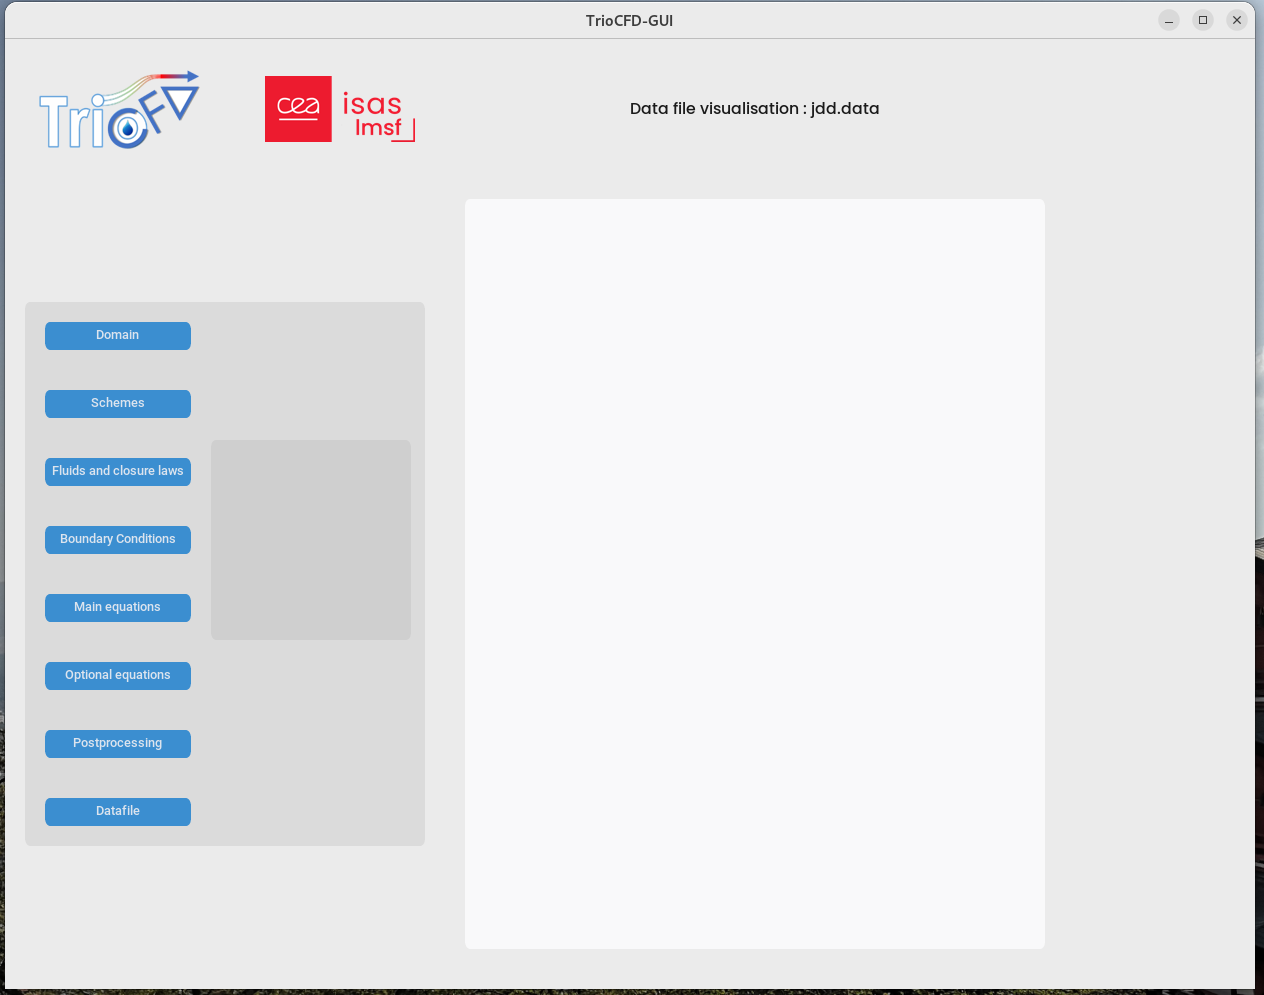
\includegraphics[scale=0.35]{Figure/GUI.png}
    \caption{Visualization of TrioCFD multiphase GUI.}
    \label{GUI}
\end{figure}
The GUI is coded in Python and may require the installation of the following packages: customtkinter, tkinter, and PIL. To launch the GUI, please find yourself in the right folder and do the command : python3 GUI. Its straightforward approach is based on reading and writing files, allowing users to fill in the data file step by step without loosing every files. Generally, users just need to click as many blue buttons as possible. However, red buttons should be used with caution. To complete the file, simply interact with all the buttons on the left side of the main interface. Don't forget to save at each submenu and to push the End datafile button when finished. The data file visualization window on the right is especially useful for checking that the data file is being filled out correctly.
\begin{figure}[htbp] 
\centering 
\begin{subfigure}[b]{0.45\textwidth} 
\centering 
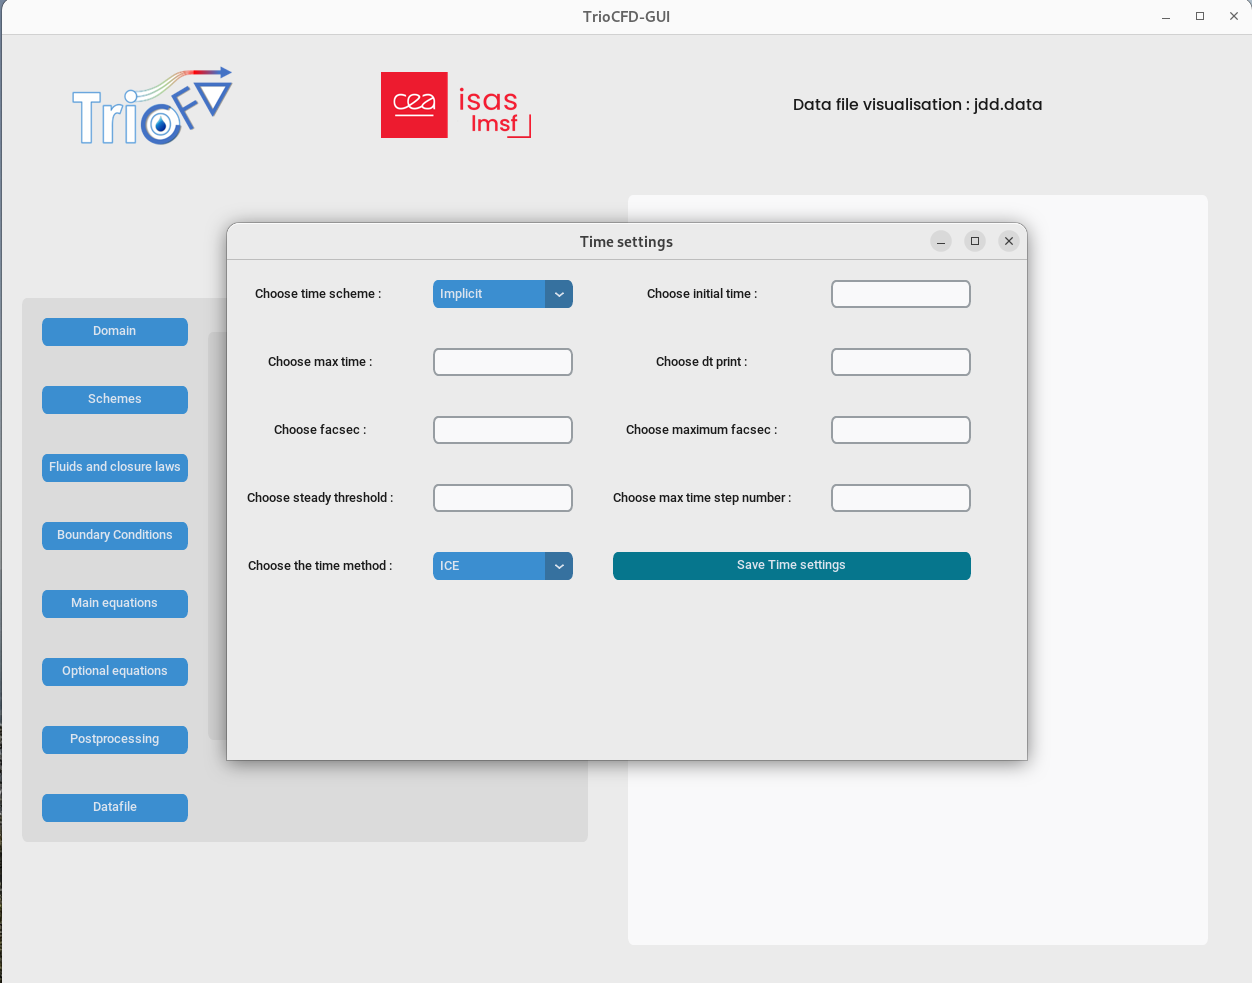
\includegraphics[scale=0.2]{Figure/Guitime.png} 
\caption{Time settings of GUI.}  
\end{subfigure} 
\hfill 
\begin{subfigure}[b]{0.45\textwidth} 
\centering 
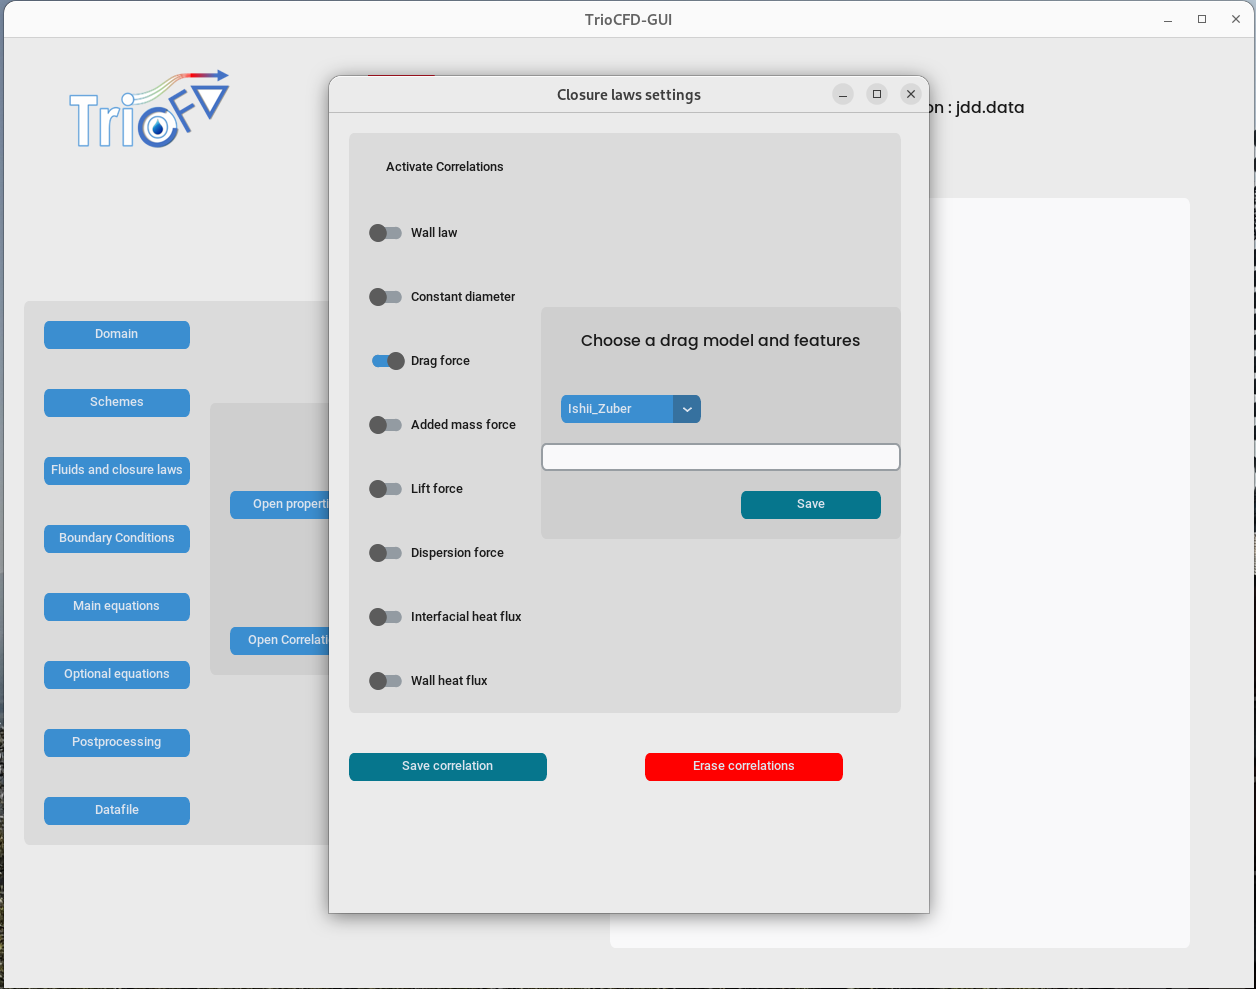
\includegraphics[scale=0.2]{Figure/Guicorrel.png} 
\caption{Closure laws of GUI.} 
 \end{subfigure} \\[1ex] 
\begin{subfigure}[b]{0.45\textwidth} 
\centering 
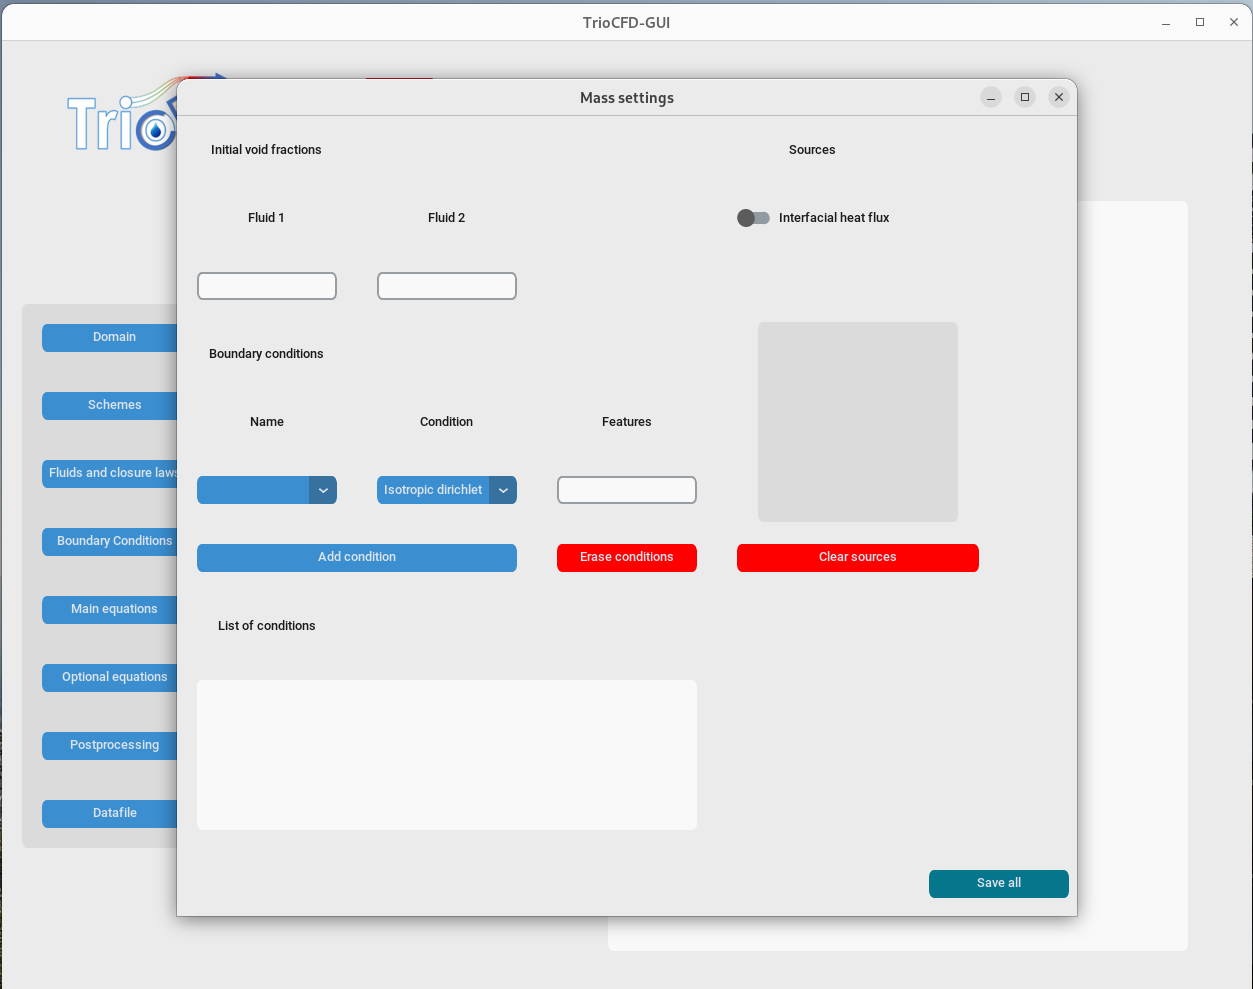
\includegraphics[scale=0.2]{Figure/Guimass.png} 
\caption{Mass equation settings of GUI.} 
\end{subfigure} \hfill 
\begin{subfigure}[b]{0.45\textwidth} 
\centering 
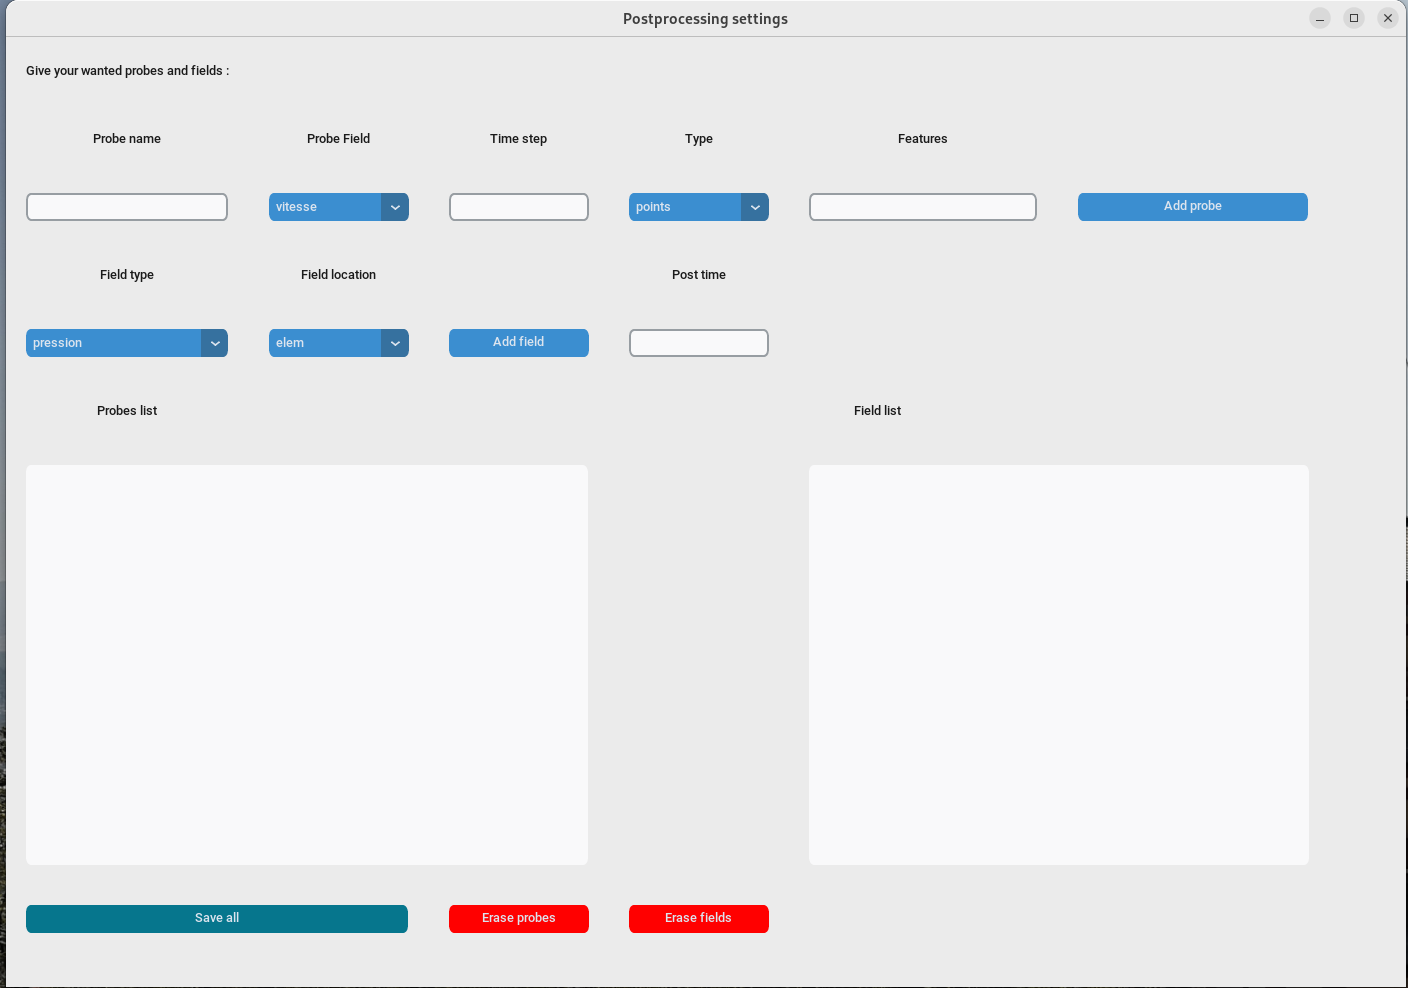
\includegraphics[scale=0.175]{Figure/Guipost.png} 
\caption{Post-processing settings of GUI.}  
\end{subfigure} 
\caption{Snapshots of different sub-menus of the GUI.}  
\end{figure} 
\cleardoublepage

% Mix informatique/numérique
%%%%%%%%%%%%%%%%%%%%%%
\chapter{Evanescence operator}\label{sec:evanescence}
This chapter aims to explain a class that is central to the management of phases and models in TrioCFD multiphase: the evanescence operator. The first section serves to establish the basic vocabulary and concepts related to the operator (section \ref{eva:obj}). The next three sections explain the operator's action on the momentum (section \ref{sec:evan-ope-and-mom}) and energy equations (section \ref{sec:evan-ope-and-nrj}) as well as a specific explanation of flux management (section \ref{sec:flux-limiter}). The last two sections focus on how this function is called in datasets (\ref{sec:eva-dataset}) and the basics of their implementation in the code (section \ref{eva:coding}).
%%%%%%%%%%%%%%%%%%%%%%
\section{Objectives}\label{eva:obj}

Evanescence is an operator in term of TRUST library. This operator can be apply to the momentum or energy equation, it consists in a relaxation of a minority phase property (\textit{i.e.} velocity or temperature) toward the property of a so-called predominant phase. 
Evanescence operator is systematically attached in the data-set to the momentum equation to ensure numerical stability.
It is optional in the energy equation. 
The following sections explain the purpose of this operator, the data-set syntax and some details about its implementation. Evanescence operator is defined whatever the number of phases so the following explanations are generic. Nevertheless, it is necessary to define the following phases:
\begin{itemize}
    \item the minority phase identified by the subscript \textit{mino},
    \item the predominant phase identified by the subscript \textit{pred} 
    \item and \textit{i} refers to a non-specific phase.
\end{itemize} 
This chapter deals with all the aspects link to the evanescence operator. It is organized as follow. The relaxation of the momentum and energy equations are detailed in section~\ref{sec:evan-ope-and-mom} and \ref{sec:evan-ope-and-nrj} respectively. Section~\ref{sec:flux-limiter} explains the process allowing to limit the interface face flux to avoid e negative volume fraction. Finally, sections~\ref{sec:eva-dataset} and \ref{eva:coding} give information on the setup and coding of the evanescence process.

%%%%%%%%%%%%%%%%%%%%%%
\section{Evanescence operator and momentum equation\label{sec:evan-ope-and-mom}}

The multiphase resolution of TrioCFD is based on a non-conservative form of the momentum transport equations as $v_i$ is evaluated instead of $\alpha_i \rho_i  v_i$. This specificity can leads to important divergence of the velocity if the void fraction $\alpha_i$ becomes locally low.
Evanescence operation can be applied to the momentum equation to overcome this difficulty. 
It enforces the coherence between the minority and the predominant phases by imposing a relation between the velocities of the minority phase and predominant phases. 
It also works if $\alpha_{k} = 0$ locally, even though in this case the momentum of the minority phase is zero. 
Thus, it is necessary to enforce a specific relation on the minority phase velocity $v_{\text{mino}}=v_{\text{pred}}+v_{\text{drift}}$. 
By default $v_{\text{drift}}$ is null, but this value can be set through a correlation (see section~\ref{sec:phyical_modeling}). 
To parameterize the relaxation of $v_{\text{mino}}$ with respect to $v_{\text{pred}}$, it is necessary to define a threshold value of alpha beyond which a minority phase can be identified as null. 
This value is noted $\alpha_{\text{res,min}}$. 
By essence, the condition $\alpha_i<\alpha_{\text{res,min}}$ can occur intermittently both spatially and temporally. 
To prevent numerical instabilities, a second threshold $\alpha_{\text{res}}$ is defined to relax $v_{\text{mino}}$ toward $v_{\text{pred}}+v_{\text{drift}}$. 
By definition, this second threshold $\alpha_{\text{res}}$ must be higher than $\alpha_{\text{res,min}}$. 
This operation can be highlight in a mathematical framework considering $\mathcal{Q}_i$ the momentum of a the $i^{th}$ phase 
\begin{equation}
\label{eq:evanescence_momentum}
\begin{pmatrix}
{\mathcal{Q}_{\text{pred}}}  \\
{\mathcal{Q}_{\text{mino}}}
\end{pmatrix}
\Longrightarrow
\begin{pmatrix}
\mathcal{Q}_{\text{pred}} + c \mathcal{Q}_{\text{mino}} - c \parent{v_{\text{mino}}=v_{\text{pred}} + v_{\text{drift}}} \\
\parent{1 - c} \mathcal{Q}_{\text{mino}} + c \parent{v_{\text{mino}}=v_{\text{pred}} + v_{\text{drift}}}
\end{pmatrix}
\end{equation}
with $c$ defined as
%\begin{equation}
    %\label{eq:evanescence_relaxation}
    %c= \textrm{min}\left(1,\textrm{max}\left(0,\frac{\alpha}{\alpha_{\textrm{res,min}}-\alpha_{\textrm{res}}}+ %\frac{\alpha_{\textrm{res}}}{\alpha_{\textrm{res}}-\alpha_{\textrm{res,min}}} \right) \right) \; .
%\end{equation}
\begin{equation}
    \label{eq:evanescence_relaxation}
    c = \text{min}\parent{1,\ \text{max} \parent{0,\ \frac{\alpha_{\text{res}}-\alpha_{\text{min}}}{\alpha_{\text{res,min}}-\alpha_{\text{res}}}}}.
\end{equation}
The evolution of the parameter $c$ is illustrated Figure~\ref{fig:evanescence_relaxation}. This operator is coded within the class \texttt{Op\_Evanescence\_Homogene\_Face\_base} in TRUST.

\begin{figure}[ht]
  \centering
\begin{tikzpicture}
  \draw[->] (0, 0) -- (0, 3);
  \draw[->] (0, 0) -- (5, 0);

  \draw (0, 2) -- (2, 2) -- (4, 0);
  \draw[dashed] (2, 0) -- (2, 2);

  \node[below] at (4, 0) {$\alpha_{\text{res}}$};
  \node[below] at (2, 0) {$\alpha_{\text{res,min}}$};
  \node[below right] at (5, 0) {$\alpha_{\text{mino}}$};

  \node[left] at (0, 0) {0};
  \node[left] at (0, 2) {1};
  \node[above left] at (0, 3) {c};
\end{tikzpicture}
  %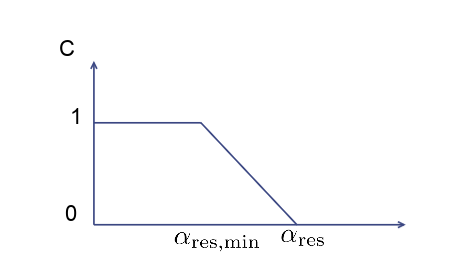
\includegraphics[width=.49\textwidth]{Figure/evanescenceRelaxation.png}
  \caption{Evolution of the coefficient $c$ as a function of $\alpha_{\text{mino}}$.}
  \label{fig:evanescence_relaxation}
\end{figure}

Considering the evolution of the coefficient, the system~\ref{eq:evanescence_relaxation} can be described as follow:
\begin{itemize}
    \item $\alpha_{\text{res}} < \alpha_{\text{mino}}$ : the system is unchanged.
    \item $\alpha_{\text{res,min}} < \alpha_{\text{mino}} < \alpha_{\text{res}}$: partial relaxation of the velocity of the minority phase toward the velocity of the majority phase. The momentum equation solved for the minority phase is a relaxation equation that brings the velocity of the minority phase to that of the majority phase.
    \item $\alpha_{\text{mino}} < \alpha_{\text{res,min}}$: the system is fully reduced by summing the momentum equation of $\alpha_{\text{mino}}$ with $\alpha_{\text{pred}}$. 
\end{itemize}

In other words, when $\alpha$ of the minority phase is less than $\texttt{alpha\_res\_min}$ (i.e., $c=1$), we are in pure HEM, whereas when $\alpha$ of the minority phase is greater than $\texttt{alpha\_res}$, we are in the Two-fluid model. Thus, when we are between the two, we are in a linear combination of the two cases (relaxation) to avoid making the transition abruptly. It should also be noted that in the case of a two-phase system, the minority phase is defined by $\alpha<0.5$. Therefore, if we take $\texttt{alpha\_res}$=1 and $\texttt{alpha\_res\_min}$=0.5 with 2 phases, it means we are always in HEM for the minority phase because $\alpha<0.5$ for the minority phase is always satisfied with 2 phases. However, if we only want to avoid velocity problems with the minority phase when it tends to disappear, we rather impose $\texttt{alpha\_res}=\num{1.e-6}$ (arbitrary pseudo-zero) and $\texttt{alpha\_res\_min}=\num{5.e-7}$ (slightly lower to smooth the transition to HEM), this is ultimately equivalent to having a single-phase system.

This operation is implemented through the object \texttt{correlation}. 
Equation~\ref{eq:evanescence_relaxation} is an example of a correlation that can be used. 
Correlations related to the momentum equations are documented in~\ref{sec:phyical_modeling_drift_velocity} and correlation link to the energy equations are documented in~\ref{sec:phyical_modeling_interface_heat_flux}.

%%%%%%%%%%%%%%%%%%%%%%
\section{Evanescence operator and energy equation\label{sec:evan-ope-and-nrj}}

As reminder, the energy equations for the minority phase reads
\begin{multline}
    \label{eq:eva_energy}
    \frac{\partial \alpha_{\text{mino}} \rho_{\text{mino}} h_{\text{mino}}}{\partial t}+\nabla \cdot\left(\alpha_{\text{mino}} \rho_{\text{mino}} h_{\text{mino}} \vec{v}_{\text{\text{mino}}}\right)=-p\left[\frac{\partial \alpha_{\text{mino}}}{\partial t} +\nabla \cdot\left(\alpha_{\text{mino}} \vec{v}_{\text{mino}}\right)\right] \\
    +\nabla \cdot\left(\alpha_{\text{mino}} \lambda_{\text{mino}} \nabla T_{\text{mino}}\right)+q_{\text{mino,p}}+q_{\text{mino,i}}
\end{multline}
where $q_{\text{mino},i}$ the interfacial flux, $q_{\text{mino},p}$ the parietal flux (to evaluate the diffusive flux near wall boundary conditions). This parietal flux $q_{\text{mino},p}$ can be linked to the mass interface flux $\Gamma_i$ thought a correlation. In this case, they are linked as follow
\begin{equation}
    \Gamma_g = -\Gamma_l = \frac{q_{l} + q_{g}}{L_{\text{vap}}},
\end{equation}
with $L_{\text{vap}}$ the vaporisation enthalpy. For the same reason as mentioned in the previous section, the problem can be ill-posed if the minority phase tends toward zero. For this reason, the evanescence operator can be applied to the energies equations. We obtain the same system than for the momentum one :
\begin{equation}
\label{eq:evanescence_nrj}
\begin{pmatrix}
{\mathcal{E}_{\text{pred}}}  \\
{\mathcal{E}_{\text{mino}}}
\end{pmatrix}
\Longrightarrow
\begin{pmatrix}
{\mathcal{E}_{\text{pred}}} + c {\mathcal{E}_{\text{mino}}} - c \parent{T_{\text{mino}}=T_{\text{pred}}+T_{\text{corr}}} \\
\parent{1 - c} {\mathcal{E}_{\text{mino}}} + c \parent{T_{\text{mino}}=T_{\text{pred}}+T_{\text{corr}}}
\end{pmatrix}
\end{equation}

Similarly to the momentum equation, it is necessary to define a relevant minority phase temperature in the case that $\alpha_{\text{mino}}$ is too low. In this case, it is important to define $T_{\text{mino}}$. Two scenarios may arise:
\begin{description}
    \item[No phase change ($\Gamma_{\text{mino}}=0$):] in this case $q_{\text{mino},i}= h \parent{T_{\text{mino}}-T_{\text{mino,sat}}}$ (with $h$ the heat transfer coefficient) and there is no need of evanescence operator if $h$ does not tend toward zero.
    % 16'
    \item[Considering phase change ($\Gamma_{\text{mino}} \neq 0$):] in this case $q_{\text{mino}} = h \parent{T_{\text{mino}}-T_{\text{mino,sat}}} + \Gamma_{\text{mino}} h_{\text{mino}}$. The term $\Gamma_{\text{mino}} h_{\text{mino}}$ is related to the default of energy due to mass transfer at the interface. It must be noted that if $\Gamma_{\text{mino}} > 0$ then $h_{\text{mino}} = h_{\text{mino,sat}}$. The underlying idea is that the phase is created from an interface at saturation temperature. This specificity is well documented in CATHARE documentation~\cite{dummycitation}. It aims at avoiding that vapour condensate considering too low latent heat and stay to high. 
\end{description}
It has to be precised that $T_{\text{mino}}$ can be imposed at $T_{\text{sat}}$ if the composite medium is at saturation.
% Il y a dissymétrie ici. Le traitement spécifique de h en fonction du signe de $\Gamma_k$ est pensé de façon à ce que la vapeur soit la phase minoritaire. Vérifier ça avec Antoine ou Corentin.


%%%%%%%%%%%%%%%%%%%%%%
\section{Flux limiter\label{sec:flux-limiter}} %19'

%First thermodynamic principle at resolved scales:
%\begin{equation}
%    \Gamma_{k} L_v = [ \lambda \nabla T] \; .
%\end{equation}
The source term $\Gamma_{k}$ has to respect two conditions:
\begin{enumerate}
    \item flux consistency: $q_{k i} + q_{k i} =0$
    \item positive volume fractions for each phase: $\alpha_i(\boldsymbol{x},t) \; \forall \; \boldsymbol{x} \; \textrm{and} \ t $. 
\end{enumerate}
To achieve this goal, a first estimation of the interfacial heat flux is calculated from correlations for each phase:
\begin{equation}
    \label{eq:evanescence_clipping}
    \Gamma_{k} = f(q_{i}) \; \text{such as} \; q_{\text{mino}} + q_{\text{pred}} = 0.
\end{equation}
Then a flux limiter is calculated from the transport equation of the minority phase:
\begin{equation}
    \label{eq:evanescence_Glim}
    \Gamma_{\text{lim}}=\nabla \cdot (\alpha_{\text{mino}}\rho_{\text{mino}})\overrightarrow{v}_{\text{mino}}-\frac{\partial \alpha_{\text{mino}}\rho_{\text{mino}}}{\partial t}.
\end{equation}
If $\Gamma_{k} < \Gamma_{\text{lim}}$ both conditions are respected. 

However, if $\Gamma_{k} \geq \Gamma_{\text{lim}}$, the resulting volume fraction of the minority phase would be negative. 
In this case, $\Gamma_{k}$ is imposed at $\Gamma_{\text{lim}}$ value and the flux consistence is imposed through the following relations
\begin{align}
    q_{\text{mino}} &= h \left( T_{\text{mino}}-T_{\textrm{mino,sat}} \right) + \Gamma_{\text{lim}} h_{\text{mino}},\\
    q_{\text{pred}} &= -q_{\text{mino}}.
\end{align}
These operations are coded in file \texttt{Source\_Flux\_interfacial\_base}.

%%%%%%%%%%%%%%%%%%%%%%
\section{Dataset\label{sec:eva-dataset}}

An example of evanescence operator is 
\begin{lstlisting}[caption={data set definition},captionpos=b,escapechar=|]
    QDM_Multiphase
    {
        evanescence { homogene { alpha_res 1.e-6 alpha_res_min 5.e-7 } }
        solveur_pression petsc cli_quiet { -pc_type hypre -pc_hypre_type boomeramg -ksp_type fgmres }
        convection { amont }
        diffusion  { turbulente $diffusion { sigma 1 } }
        initial_conditions
        {
            ...
        }
        conditions_limites
        {
            ...
        }
    }
\end{lstlisting}
with \texttt{alpha\_res} corresponding to $\alpha_{\textrm{min}}$ and \texttt{alpha\_res\_min} corresponding to $\alpha_{\textrm{res,min}}$.


%%%%%%%%%%%%%%%%%%%%%%
\section{Coding\label{eva:coding}}

\subsection{Faces}
\begin{itemize}
    \item[\small \textcolor{blue}{\ding{109}}]\texttt{Op\_Evanescence\_Homogene\_Face\_base}: management for faces (linked to momentum equation and so can impose the drift velocity) 
\end{itemize}
The model is implemented in 2 files.
\begin{lstlisting}[language=c++]
void Op_Evanescence_Homogene_Elem_base::readOn(Entree& is)
{
  Param param(que_suis_je());
  param.ajouter("alpha_res", &alpha_res_, Param::REQUIRED);
  param.ajouter("alpha_res_min", &alpha_res_min_);
  param.lire_avec_accolades_depuis(is);
  return is;
}
\end{lstlisting}

\subsection{Elements}

\begin{itemize}
    \item[\small \textcolor{blue}{\ding{109}}]\texttt{Op\_Evanescence\_Homogene\_Elem\_base}: management for elements (linked to mass and energy equations and can weakly imposed conditions for temperature and void fraction, based on fluxes)
\end{itemize}
\begin{lstlisting}[language=c++]
void Op_Evanescence_Homogene_Face_base::readOn(Entree& is)
{
  Param param(que_suis_je());
  param.ajouter("alpha_res", &alpha_res_, Param::REQUIRED);
  param.ajouter("alpha_res_min", &alpha_res_min_);
  param.lire_avec_accolades_depuis(is);

  Pb_Multiphase& pbm = ref_cast(Pb_Multiphase, equation().probleme());
  if (pbm.has_correlation("Vitesse_relative") && !pbm.has_correlation("gravite")) Process::exit(que_suis_je() + " : you must define a multiphase gravity field if you want a drift flux!!");
  if (pbm.has_correlation("Vitesse_relative") && ref_cast(Vitesse_relative_base, pbm.get_correlation("Vitesse_relative").valeur()).needs_vort()) pbm.creer_champ("vorticite");

  return is;
}
\end{lstlisting}

Default values : \texttt{alpha\_res\_} = 0, \texttt{alpha\_res\_min\_} = 0.

\subsection{Implementation}

The model is called for each dimensioning and assembly of blocks or matrices (\texttt{assembler\_blocs}, \texttt{dimensionner\_forblocs}, \texttt{dimensionner\_matrice}). 
It allows adding the equation of the residual phase to the majority phase, locally according to a global criterion \texttt{alpha\_res\_}. 
It is possible to impose an algebraic relationship for velocity and temperature (i.e., $v_l = v_g$ or $v_l = v_g + v_r$ for velocity, $T_l = T_{\text{sat}}$ or $T_l = T_g$ for temperature). 
Conditions on void fraction and temperature are imposed through flux corrections in the mass and energy equations. 
For example, for mass equation:
\begin{equation}
\Gamma_{k,\text{mino}}=\nabla \cdot (\alpha_k\rho_k)\overrightarrow{v_k} - \frac{\partial \alpha_k\rho_k}{\partial t}
\end{equation}
In the case of the energy equation, if the flux is imposed by a correlation, then it is the pressure term that is corrected.

It is implemented as:
\begin{itemize}
\item[\small \textcolor{blue}{\ding{109}}]For elements and faces \texttt{secmem(e, k)} adds corrected flux in right hand side of the equation of local main phase,
\item[\small \textcolor{blue}{\ding{109}}]For elements and faces \texttt{secmem(e, n)} corrects the flux in right hand side of the equation of local evanescent phase,
\item[\small \textcolor{blue}{\ding{109}}]For faces, if a drift velocity model is defined with \texttt{correlation\_vd}, we impose the relative velocity between the local main phase and the local evanescent phase,
\end{itemize}
with \texttt{e} elements, \texttt{k} majority local phase, \texttt{n} evanescent local phase.

%%%%%%%%%%%%%%%%%%%%%%
%\section{Pb_Multiphase_HEM}
%The keyword $Pb\_ Multiphase\_ HEM$ enables the use of a HEM model through $Pb\_ multiphase$. It allows the resolution of $2$ phases mechanicaly and thermally coupled with one common set of equations (mass, momentum and energy). It notably uses $Evanescence\_ Homogene$ to achieve this. It is equivalent to the following line in the data set :
%\begin{lstlisting}[language=c++]
%evanescence { homogene { alpha_res 1 alpha_res_min 0.5 } }
%\end{lstlisting}
%If this keyword is used, it is mandatory to associate an interfacial flux correlation with constant coefficient.

\cleardoublepage
\chapter{Time schemes}
\label{sec:time_scheme}
This chapter aims to describe the different time schemes available for TrioCFD multiphase computations. The first section (\ref{time:preambule}) is an introduction to the time stepping general methods before delving into the ICE/SETS method (section \ref{time:ice}) and the future PAT method (section \ref{time:pat}).
\section{Preamble}\label{time:preambule}
Compressible codes fall into two categories based on their approach to solving the compressible Navier-Stokes equations. The first category comprises density-based methods, which are commonly employed for modeling flows dominated by acoustic phenomena or fluid compressibility effects. These methods aim to directly solve the compressible form of the Navier-Stokes equations, closing the system by computing thermodynamic pressure through an equation of state. However, density-based solvers face a drawback in low-Mach number flow modeling due to their explicit time integration approach. 
The main drawback of density-based solvers in the context of low-Mach number flow modeling is their explicit time integration of the governing equation system. When fluid flow is modeled with a fully explicit method, time-step sizes are restricted by the local Courant-Friedrichs-Lewy limit as:
\begin{equation}
    \label{eq:time_step_compressible1}
    \Delta_{t,acs} \leq \frac{k \Delta_x}{\mid u\mid + c} \; ,
\end{equation}
with $k$ a constant depending of the numerical scheme, $c$ the sound speed and $u$ the velocity. Because of the significant difference between the entropy and the acoustic wave propagation speeds in low-Mach number flows, the explicit resolution of these phenomena is poorly optimized in low-Mach cases. Indeed, defining a convective acoustic time step as 
\begin{equation}
    \label{eq:time_step_compressible2}
    \Delta_{t,conv} \leq \frac{k \Delta_x}{\mid u\mid} \; ,
\end{equation}
it leads to the relation
\begin{equation}
    \label{eq:time_step_compressible3}
    \Delta_{t,acs} = \Delta_{t,conv} \frac{\mathcal{M}_a}{1+ \mathcal{M}_a} \; ,
\end{equation}
with $\mathcal{M}_a$ the local Mach number. $\Delta_{t,acs} \ll \Delta_{t,conv}$ if $\mathcal{M}_a \ll 1$.

To overcome this difficulty pressure-based methods have been developed. In contrast to density-based methods, which solve the Navier-Stokes equation for density and compute the pressure thanks to an equation of state, the main idea of pressure-based methods is to use the pressure gradient as a constraint on the velocity in the momentum equations. The pressure gradient, calculated from a Helmholtz-type wave equation, has thus the great advantage of remaining finite in low-Mach number flows. Hence, such methods are commonly used to compute compressible phenomena in low-Mach number flows. 
This section presents the two pressure-based methods available within CFMD called ICE (Implicit Continuity Equation) and initially developed by \cite{harlow1968numerical,harlow1971numerical}. It is a pressure-based approach used in solving the Navier-Stokes equations for numerical simulation of fluid flows. 

%%%%%%%%%%%%%%%%%%%%%%%%%%%%%%%
\section{The ICE/SETS methods} \label{time:ice}
All the temporal schemes available with the \texttt{Pb\textunderscore multiphase} problem belong to the SETS class. ICE temporal scheme is a sub-class of SETS class.\\ The class ICE inherits from the SETS class. Both classes share the same parameters that are listed below.
\begin{lstlisting}
int p_degen = -1
\end{lstlisting}
If \texttt{SETS.p\textunderscore degen} is equal to -1, the numerical schem is corresponding to a semi-implicit scheme.\\ If \texttt{SETS.p\textunderscore degen} is equal to 1, the numerical scheme is corresponding to an incompressible solver. In this case, the pressure has a relative value: no BC can be impose on the pressure and no compressibility effects are considered.

\subsection{Description of the algorithm}
The keyword to activate the \textsc{ice} method in a multiphase computation in TrioCFD is \lstinline{solver ICE}. The algorithm is implemented in the \texttt{SETS.cpp} file as it is closely related to the \textsc{sets} method. This algorithm carries two main functions that are used to solve the equations, namely \texttt{iterer_eqn} and \texttt{iterer_NS}. The first is use to iterate all equations in time and the second uses a Newton method to solve the momentum equation on velocity with pressure reduction. We briefly describe the algorithm of both function.
% \begin{lstlisting}[language=c++]
% void iterer_eqn // Equation iteration
% \end{lstlisting}
\paragraph{General algorithm for every equation}\mbox{}\\
\begin{algorithm}[H]
  \SetAlgoLined
  \KwIn{Unknowns: void fraction (always), temperature (ICE), standard convection-diffusion quantities (for example turbulence or IATE, ICE)}
  \KwOut{Updated unknowns}
  
  \BlankLine
  \textbf{Step 1: Positivity Enforcement}\;
  \ForEach{unknown}{
    \eIf{unknown is positive}{
      Update current unknown via increment\;
    }{
      Impose 0 (via unknown_positivation)\;
    }
  }
  
  \BlankLine
  \textbf{Step 2: Solve Navier-Stokes Equations}\;
  \If{Navier-Stokes equations are in the system}{
    Call iterer_NS to solve velocity and pressure\;
  }
  
  \BlankLine
  \textbf{Step 3: Solve Thermal Equation}\;
  Solve multiphase or conduction thermal equation explicitly if ICE is used\;
  
  \BlankLine
  \textbf{Step 4: Check Positivity of Temperature}\;
  Check if temperature is positive\;
  
  \BlankLine
  \textbf{Step 5: Update Time Step and Unknowns}\;
  Update time step and the unknowns\;
  
  \caption{Algorithm iterer_eqn}
\end{algorithm}

\paragraph{Specific algorithm for the momentum and pressure equations}\mbox{}\\
\begin{algorithm}[H]
  \SetAlgoLined
  \KwIn{Initial values}
  \KwOut{Updated values}
  
  \BlankLine
  \textbf{Step 1: Initialization}\;
  Save current values in the past\;
  
  \BlankLine
  \textbf{Step 2: Solve Velocity}\;
  \eIf{SETS is activated}{
    Solve velocity with explicit pressure and store it\;
  }{
    Save past value of velocity\;
  }
  
  \BlankLine
  \textbf{Step 3: PolyMAC Correction}\;
  \If{PolyMAC is active}{
    Correct velocity at elements using mass\;
  }
  
  \BlankLine
  \textbf{Step 4: Newton Method}\;
  \textbf{Step 4.1:} Fill energy equation to obtain wall transfers\;
  \textbf{Step 4.2:} Fill other equations\;
  \textbf{Step 4.3:} Assemble pressure system\;
  \eIf{pressure reduction}{
    \textbf{Step 4.4.1:} Eliminate unknowns for $A_p$ and $b_p$ for each phase by substitution\;
    \textbf{Step 4.4.2:} Assemble system $A_p$ and $B_p$\;
    \textbf{Step 4.4.3:} Solve pressure\;
    \textbf{Step 4.4.4:} Solve other increments\;
  }{
    \textbf{Step 4.5:} Solve directly by \texttt{mat_semi_impl}\;
  }
  \textbf{Step 4.6:} If PolyMAC, apply mass correction to correct velocity at elements\;
  
  \BlankLine
  \textbf{Step 5: Convergence Check}\;
  Convergence criteria (see Table~\ref{tab:convergence} for default criteria)\;
  
  \BlankLine
  \textbf{Step 6: Update}\;
  Update values\;
  
  \caption{Algorithm for iterer_NS}
\end{algorithm}

\begin{table}[!h]
    \centering
       \begin{tabular}{c c c}
        \toprule
        Field & Notation & Criteria   \\
        \midrule
        \rowcolor[gray]{0.9} Void fraction & $\alpha$  & $0.01$  \\
        Temperature & $T$  & $0.1$ \\
        \rowcolor[gray]{0.9} Velocity & $v$ &  $0.01$ \\
        Pressure & $p$  &  $100$\\
        \rowcolor[gray]{0.9} Turbulent kinetic energy & $k$   &  $0.01$\\
        Wake induced turbulent energy & $k_{WIT}$ &   $0.01$\\
        \rowcolor[gray]{0.9} Rate of dissipation & $\omega$  &  $0.01$\\
        Dissipation time scale & $\tau$  &  $0.01$ \\
        \rowcolor[gray]{0.9} Interfacial area concentration & $ai$ &  $100$ \\
        \bottomrule
    \end{tabular}
    \caption{Default convergence criteria}
    \label{tab:convergence}
\end{table} 

\subsection{Principle of the time discretization}
The following steps are also presented in \cite{GerschenfeldPolyMAC2022}. \\
We can write the time discretized mass, momentum and energy conservation equations along with the continuity axiom:
% \begin{equation}
% \begin{aligned}
% (\mathcal{M}_k) \hspace{1cm}
% 		\frac{ {\color{red} \alpha_k^{n+1} \rho_k^{n+1}}-\alpha_k^{n} \rho_k^{n}}{\Delta t} +\nabla \cdot ({\alpha_k^{n} \rho_k^{n}} {\color{red}  \vec{v_k}^{n+1}})
% 		= {\color{red} \Gamma_k^{n+1}}  
% \end{aligned}
% \end{equation}
% \begin{equation}
% \begin{aligned}
% (\mathcal{Q}_k) \hspace{1cm}
% 		\alpha_k^{n} \rho_k^{n}\frac{{\color{red}\vec{v_k}^{n+1}}-\vec{v_k}^{n}}{\Delta t} + \underline{\nabla} \cdot ({\alpha_k^{n} \rho_k^{n} \vec{v_k}^{n}} \otimes \vec{v_k}^{n})-\vec{v_k}^{n}\underline{\nabla} \cdot (\alpha_k^{n} \rho_k^{n} \vec{v_k}^{n})
% 		= &  -\alpha_k^{n} \underline{\nabla} {\color{red}P^{n+1}}  +
% 		 \underline{\nabla} \cdot (\alpha_k^{n} \mu_k^{n} \underline{\underline{\nabla}} \vec{u_k}^{n}) \\ & - \underline{\nabla} \cdot  (\alpha_k^{n}\rho_k^{n} \overline{u_i'u_j'}^{n}) 
% 		 + {\color{red}\vec{F}_{ki}^{n+1}}
% 		+ {\color{red}\vec{F}_k^{n+1}}
% \end{aligned}
% \end{equation}
% \begin{equation}
% \begin{aligned}
% 		(\mathcal{E}_k) \hspace{1cm} \frac{ {\color{red}\alpha_k^{n+1} \rho_k^{n+1} e_k^{n+1}}-\alpha_k^{n} \rho_k^{n} e_k^{n}}{\Delta t} + \nabla \cdot ({\alpha_k^{n} \rho_k^{n} e_k^{n}} {\color{red}\vec{v_k^{n+1}}}) = & 
% 		 \nabla \cdot [ \alpha_k^{n}\lambda_k \underline{\nabla} T^{n}  - \alpha_k^{n}\rho_k^{n} \overline{u_i'e_k'}^{n}] + q_{ki}^{n} +
% 		q_{kp}^{n} \\
% 		& -{\color{red}P^{n+1}} \left[\frac{{\color{red}\alpha_k^{n+1}}-\alpha_k^n}{\Delta t} + \nabla \cdot (\alpha_k^{n} {\color{red}\vec{v_k^{n+1}}})\right]& &
% \end{aligned}
% \end{equation}

\begin{align}
& (\mathcal{C}) && \sum_k  {\color{red} \alpha_k^{n+1}}=1 \label{eq:discAlphak}\\
& (\mathcal{M}_k) && \frac{ {\color{red} \alpha_k^{n+1} \rho_k^{n+1}}-\alpha_k^{n} \rho_k^{n}}{\Delta t} +\nabla \cdot ({\alpha_k^{n} \rho_k^{n}} {\color{red}  \vec{u_k}^{n+1}}) = {\color{red} \Gamma_k^{n+1}}\label{eq:discMk}\\
&(\mathcal{Q}_k) &&
  \begin{multlined}[c][0.8\linewidth]
    \alpha_k^{n} \rho_k^{n}\frac{{\color{red}\vec{u_k}^{n+1}}-\vec{u_k}^{n}}{\Delta t} + \underline{\nabla} \cdot \parent{{\alpha_k^{n} \rho_k^{n} \vec{u_k}^{n}} \otimes \vec{u_k}^{n}}-\vec{u_k}^{n}\underline{\nabla} \cdot \parent{\alpha_k^{n} \rho_k^{n} \vec{u_k}^{n}} = \\-\alpha_k^{n} \underline{\nabla} {\color{red}P^{n+1}} + \underline{\nabla} \cdot \parent{\alpha_k^{n} \mu_k^{n} \underline{\underline{\nabla}} \vec{u_k}^{n}} \\- \underline{\nabla} \cdot  (\alpha_k^{n}\rho_k^{n} \overline{u_i'u_j'}^{n}) + {\color{red}\vec{F}_{ki}^{n+1}} + {\color{red}\vec{F}_k^{n+1}}
  \end{multlined}\label{eq:discQk}\\
&(\mathcal{E}_k) &&
  \begin{multlined}[c][0.8\linewidth]
    \frac{ {\color{red}\alpha_k^{n+1} \rho_k^{n+1} e_k^{n+1}}-\alpha_k^{n} \rho_k^{n} e_k^{n}}{\Delta t} + \nabla \cdot ({\alpha_k^{n} \rho_k^{n} e_k^{n}} {\color{red}\vec{u_k}^{n+1}}) = \\\nabla \cdot \parent{ \alpha_k^{n}\lambda_k \underline{\nabla} T_k ^{n}  - \alpha_k^{n}\rho_k^{n} \overline{u_i'e_k'}^{n}} + q_{ki}^{n} + q_{kp}^{n} \\- {\color{red}P^{n+1}} \parent{\frac{{\color{red}\alpha_k^{n+1}}-\alpha_k^n}{\Delta t} + \nabla \cdot (\alpha_k^{n} {\color{red}\vec{u_k}^{n+1}})}
  \end{multlined}\label{eq:discEk}
\end{align}
Once this system is written, one can express a matrix system in terms of increments on the unknowns. For example, for the temporal term in the mass equation:
\begin{equation}
    \frac{1}{\Delta t}\parent{{\color{red} \alpha_k^{n+1} \rho_k^{n+1}}-\alpha_k^{n} \rho_k^{n}} = \frac{1}{\Delta t}\parent{{\rho_k^{n}}({\color{red} \alpha_k^{n+1}}-\alpha_k^{n}}+{\color{red} \alpha_k^{n+1}}\parent{{\color{red} \rho_k^{n+1}}-\rho_k^{n})+\alpha_k^{n} \rho_k^{n}-\alpha_k^{n} \rho_k^{n}}
\end{equation}
Let's remind that the unknowns are $(\alpha,\ T,\ P,\ \vec{u})$. Then, the void fraction increment is ${\color{red}\delta \alpha_k}={\color{red}\alpha_k^{n+1}}-\alpha_k^{n}$. 
For the density, one must add its dependencies to the unknowns. In this case, the density field $\rho(T,P)$ depends only on the temperature and the pressure fields. Also its differential is $d\rho= \frac{\partial \rho}{\partial T}\delta T + \frac{\partial \rho}{\partial P}\delta P$. Thus we obtain the following equation for the increments:
\begin{equation}
    \underbrace{\frac{{ \rho_k^{n}}}{\Delta t}}_{ \frac{\partial \mathcal{M}_k}{\partial \alpha_k}^{(n)}}{\color{red} \delta \alpha_k}+\underbrace{\frac{\color{red}\alpha_k^{n+1}}{\Delta t} \parent{\frac{d\rho_k}{dT_k}}^n}_{\color{red} \frac{\partial \mathcal{M}_k}{\partial T_k}^{(n+1)}} {\color{red} \delta T_k}+\underbrace{\frac{\color{red}\alpha_k^{n+1}}{\Delta t} \parent{\frac{d\rho_k}{dP}}^n }_{\color{red} \frac{\partial \mathcal{M}_k}{\partial P}^{(n+1)}}{\color{red} \delta P}
\end{equation}
We can then do this for all terms and construct the following system for the increments of unknowns:
\begin{equation}
\begin{pmatrix}
\colorboxed{OPblue!50}{\frac{\partial \mathcal{M}_k}{\partial \alpha_k}^{(n)}} & \colorboxed{OPblue!50}{\color{red} \frac{\partial \mathcal{M}_k}{\partial T_k}^{(n+1)}} & \frac{\partial \mathcal{M}_k}{\partial \overrightarrow{u_k}}^{(n)} & {\color{red} \frac{\partial \mathcal{M}_k}{\partial P}^{(n+1)}} \\
\colorboxed{OPblue!50}{\color{red}\frac{\partial \mathcal{E}_k}{\partial \alpha_k}^{(n+1)}} & \colorboxed{OPblue!50}{\color{red}\frac{\partial \mathcal{E}_k}{\partial T_k}^{(n+1)}} & {\color{red}\frac{\partial \mathcal{E}_k}{\partial \overrightarrow{u_k}}^{(n+1)}} & \frac{\partial \mathcal{E}_k}{\partial P}^{(n)}\\
0 & 0 & \colorboxed{OPblue!50}{\frac{\partial \mathcal{Q}_k}{\partial \overrightarrow{u_k}}^{(n)}} & \frac{\partial \mathcal{Q}_k}{\partial P}^{(n)}
\end{pmatrix}\begin{pmatrix}
{\color{red} \delta\alpha_k ^{(n+1)}}={\color{red} \alpha_k^{n+1}}-\alpha_k^{n}\\
{\color{red} \delta T_k^{(n+1)}}\\
{\color{red}\delta \overrightarrow{u_k}^{(n+1)}}\\
{\color{red} \delta P^{(n+1)}}
\end{pmatrix}=\begin{pmatrix}
\delta\mathcal{M}_k^{(n)} \\
\delta\mathcal{E}_k^{(n)}\\
\delta\mathcal{Q}_k^{(n)}
\end{pmatrix}
\end{equation}
The terms framed in blue (\fcolorbox{OPblue!50}{white}{\textcolor{white}{T}}) are block diagonal because they only depend on unknowns coming from the cell in which they are computed.\\
In a Newton algorithm, one can take the first line of the system, replace unknows then adds for any phases and substracts the void fraction dependency with $\sum_k  {\color{red} \delta\alpha_k^{n+1}}=0$ and then get ${\color{red}\delta P^{(n+1)}}$. This step is called pressure reduction and is described after. The last line allows the direct prediction to get $\delta \overrightarrow{u_k}^{(n+1)}$, so that the system becomes: 
\begin{equation}
\begin{pmatrix}
{\color{red}\frac{\partial \mathcal{M}_k}{\partial \alpha_k}^{(n+1)}} & \frac{\partial \mathcal{M}_k}{\partial T_k}^{(n)} \\
{\frac{\partial \mathcal{E}_k}{\partial \alpha_k}^{(n+1)}} & {\color{red}\frac{\partial \mathcal{E}_k}{\partial T_k}^{(n+1)}} \end{pmatrix}\begin{pmatrix}
{\color{red} \delta\alpha_k ^{(n+1)}}\\
{\color{red} \delta T_k^{(n+1)}}
\end{pmatrix}=\begin{pmatrix}
\delta\mathcal{M}_k^{(n)} \\
\delta\mathcal{E}_k^{(n)}
\end{pmatrix}+\begin{pmatrix}
\frac{\partial \mathcal{M}_k}{\partial P_k}^{(n)} \\
\frac{\partial \mathcal{E}_k}{\partial P_k}^{(n)}
\end{pmatrix}\delta P^{(n+1)}+
\begin{pmatrix}
\frac{\partial \mathcal{M}_k}{\partial \overrightarrow{u_k}}^{(n)} \\
\frac{\partial \mathcal{E}_k}{\partial \overrightarrow{u_k}}^{(n+1)}
\end{pmatrix}\delta \overrightarrow{u_k}^{(n+1)}
\end{equation}
Then the temperature can be solved. The convergence criteria must be then verified. 

\subsection{Principle of the pressure reduction}
To avoid heavy notations, the subscript $k$ which refers to each phase are dropped. The previous system can be written as:
\begin{align}
    &M_{\alpha}\delta \alpha +M_T \delta T +M_u\delta u +M_p \delta P=f_M\label{eq:presredM1}\\
    &{\color{myteal}E_{\alpha}}\delta \alpha +{\color{myteal} E_T} \delta T +{\color{myteal} E_u}\delta u +{\color{myteal}E_p} \delta P={\color{myteal}f_E}\label{eq:presredE1}\\
    &{\color{mydarkorchid} Q_u} \delta u+{\color{mydarkorchid} Q_p} \delta P={\color{mydarkorchid} f_Q} \label{eq:presredQ1}
\end{align}
From equation~\eqref{eq:presredQ1}, we can express the velocity increment as 
\begin{equation}
\delta u = {\color{mydarkorchid}Q_u^{-1}f_Q-Q_u^{-1}Q_p}\delta P.
\end{equation}
Injecting it into the previous system, we obtain the following system
\begin{align}
    &M_{\alpha}\delta \alpha + M_T \delta T + M_u{\parent{{\color{mydarkorchid}Q_u^{-1}f_Q} - {\color{mydarkorchid} Q_u^{-1}Q_p}\delta P}} + M_p \delta P = f_M\label{eq:presredM2}\\
    &{\color{myteal} E_{\alpha}}\delta \alpha + {\color{myteal} E_T} \delta T + {\color{myteal} E_u}{\parent{{\color{mydarkorchid}Q_u^{-1}f_Q} - {\color{mydarkorchid}Q_u^{-1}Q_p}\delta P}} + {\color{myteal} E_p} \delta P = {\color{myteal}f_E}\label{eq:presredE2}
\end{align}
One can then replace the temperature from the energy equation~\eqref{eq:presredE2} in the mass equation~\eqref{eq:presredM2}:
\begin{multline}
    M_{\alpha}\delta \alpha + M_T {{\color{myteal}E_T^{-1}}\parent{{\color{myteal}-E_{\alpha}}\delta \alpha - {\color{myteal}E_u}{\parent{{\color{mydarkorchid}Q_u^{-1}f_Q} - {\color{mydarkorchid}Q_u^{-1}Q_p}\delta P}} - {\color{myteal}E_p} \delta P + {\color{myteal}f_E}}}\\
    - M_u{\parent{{\color{mydarkorchid}Q_u^{-1}f_Q} - {\color{mydarkorchid}Q_u^{-1}Q_p}\delta P}} + M_p \delta P = f_M
    %M_{\alpha}\delta \alpha +M_TE_T^{-1}(-E_{\alpha}\delta \alpha+E_vQ_v^{-1}Q_p\delta P-E_vQ_v^{-1}f_Q-E_p\delta P+f_E)-M_vQ_v^{-1}Q_p\delta P+M_vQ_v^{-1}f_Q+M_p \delta P=f_M\\
\end{multline}
We then group together terms that multiply $\delta\alpha$ and $\delta P$. We obtain: 
\begin{multline}
\underbrace{\parent{M_{\alpha} - M_T{\color{myteal}E_T^{-1}E_\alpha}}}_{K_\alpha}\delta \alpha +\underbrace{(M_T{\color{myteal}E_T^{-1}}({\color{myteal}E_u}{\color{mydarkorchid}Q_u^{-1}Q_p} - {\color{myteal}E_p}) - {\color{mydarkorchid}M_uQ_u^{-1}Q_p}+M_p)}_{K_p}\delta P=  \\\underbrace{f_M - M_u{\color{mydarkorchid}Q_u^{ - 1}f_Q} - M_T{\color{myteal} E_T^{-1}}({\color{myteal}f_E} - {\color{myteal} E_u}{\color{mydarkorchid}Q_u^{-1}f_Q})}_{K_f}\label{eq:presred3}
\end{multline}
\textbf{Remark}: if we neglect the temperature, we have a simpler system: 
\begin{equation}
    \underbrace{M_{\alpha}}_{K_\alpha}\delta \alpha +\underbrace{(M_p-{\color{mydarkorchid} M_uQ_u^{-1}Q_p})}_{K_p}\delta P= \underbrace{f_M-M_u{\color{mydarkorchid} Q_u^{-1}f_Q}}_{K_f}.\label{eq:presred4}
\end{equation}
By inverting matrix $K_\alpha$, equations~\eqref{eq:presred3} and \eqref{eq:presred4} can be rewritten as
\begin{equation}
\delta \alpha + K_\alpha^{-1}K_p\delta P=K_\alpha^{-1}K_f.\label{eq:presred5}
\end{equation}
With the axiom of continuity, i.e. by summing equation~\eqref{eq:presred5} on all phases, we obtain the final linear system of the form $Ax=B$: 
\begin{equation}
\underbrace{\sum_k (K_\alpha^{-1}K_p)_k}_{A_p}\delta P=\underbrace{\sum_k (K_\alpha^{-1}K_f)_k}_{B_p}
\end{equation}

%%%%%%%%%%%%%%%%%%%%%%%%%%%%%%%
\subsection{SETS}
The Stability-Enhancing Two-Step (SETS) \cite{MAHAFFY1982329} time resolution method offers a mean to overcome the material Courant limit, thus mitigating certain stability issues associated with time-step size. Nonetheless, this approach does introduce a higher degree of numerical diffusion. Its interest lies notably in its suitability for simulating slow transients, allowing the use of way larger time steps compared to ICE. However, in multiphase simulations the time step is still limited by the convective time step because of $\alpha$. At each time step, this method yields an intermediate time velocity, temperature and other convected quantities (turbulence, IATE) field. This is particularly advantageous because achieving a solution with mass and energy convection becomes smoother when the velocity is already pressure-balanced. This algorithm is activated through the data set with the following keyword.
\begin{lstlisting}
solveur SETS
\end{lstlisting}
The main idea is to remind that we can use an intermediate time stepping, written $\widetilde{\cdot}$, to get closer to the wanted solution: 
\begin{equation}
    \delta P=P^{n+1}-P^n= \underbrace{P^{n+1}- \widetilde{P}^{n+1}}_{\delta P^{n+1}}+\underbrace{\widetilde{P}^{n+1}-P^{n}}_{\delta \widetilde{P}}
\end{equation}
Thus we obtain:
\begin{equation}
    \delta T=T^{n+1}-T^n= \underbrace{T^{n+1}- \widetilde{T}^{n+1}}_{\delta T^{n+1}}+\underbrace{\widetilde{T}^{n+1}-T^{n}}_{\delta \widetilde{T}}
\end{equation}
\begin{equation}
    \delta u=u^{n+1}-u^n= \underbrace{u^{n+1}- \widetilde{u}^{n+1}}_{\delta u^{n+1}}+\underbrace{\widetilde{u}^{n+1}-u^{n}}_{\delta \widetilde{u}}
\end{equation}
It means that if one choose wisely the intermediate pressure, we can have a first prediction of velocity and temperature to ease the computation of convection in the Newton algorithm. In the case of SETS, using a first prediction with explicit pressure $\delta \widetilde{P}=0$ allows to predict a pressure balanced intermediate time step for the velocity and temperature.

In the alogorithm, if \texttt{facsec_diffusion_for_sets} is bigger than 0, then the facsec is chosen to impose on the diffusion time step in SETS while the total time step stays smaller than the convection time step.

In order to overcome problems of implicit convection for $\alpha$ (due to the constraint $\sum \alpha_k =1$), one solution that could be implemented is to predict the minority phases and to impose for the major phase $\alpha^{major}=1-\sum \alpha_k^{minor}$.

\subsection{Specific case of ICE modelization within single phase framework}

Initially, ICE method solves the equations for momentum and pressure simultaneously by using an implicit formulation of the continuity equation. ICE method was initially developed for single-phase flows, and the pressure reduction method relies on MAC numerical scheme~\cite{harlow1965numerical}. 
A easy way to be more familiar with ICE method is to visualize the equations in the simple case of a single-phase flow. In this specific condition, ICE method relies on the resolution of a Poisson equation based on the implicit continuity equation. The pressure field at the end of the time step, $P^{n+1}$ is calculated by  
\begin{equation}
    \label{eq:poisson_ICE}
    \frac{\delta P}{\Delta_t^2 c^2} - \Delta P = \nabla  \cdot \nabla \left( \rho \mathbf{u u} - \mathbf{\tau}\right) + \frac{\nabla  \cdot \rho \mathbf{u}}{\Delta_t} \; .
\end{equation}
From the sound speed definition the density can be updated
\begin{equation}
    \label{eq:density_update_ICE}
    \delta \rho = \frac{\delta P}{c^2}  \; .
\end{equation}
The equation of state is involved in the calculation of the sound speed $c$. Once $P^{n+1}$ and $\rho^{n+1}$ are known, the velocity can be estimated solving the transport equation of the momentum. Finally, at the end of the time step, the temperature can be calculated from $P^{n+1}$, $\rho^{n+1}$ and $\mathbf{u}^{n+1}$.
The ICE solver is robust but must respect a strong assumption $CFL\leq 1$. Note that in this method, the diffusion of the temperature is always explicit.

%%%%%%%%%%%%%%%%%%%%%%%%%%%%%%%
\section{PAT (incoming)} \label{time:pat}
The so-called PAT for $(P,\alpha, T)$ resolution is a NeptuneCFD-looklike time scheme. It is available as an alternative for PolyVEF spatial scheme, which is not optimal with ICE/SETS method. This quasi-implicit method features a velocity prediction step followed by the calculation of pressure $P$, volume fraction $\alpha$, and temperature $T$. It uses maximal implicitness while avoiding saddle points anomalies. This time scheme is not yet validated, we advise not to use it. 

%%%%%%%%%%%%%%%%%%%%%%%%%%%%%%%

\cleardoublepage
\chapter{Spatial Scheme}
\label{sec:spatial_scheme}

This chapter gives an overview of the available spatial schemes for multiphase flow in \texttt{TRUST}/\texttt{TrioCFD}. First, common notations are given at Section~\ref{sec:notation-spa-sch}. The different schemes of the PolyMAC family are described in Section~\ref{sec:polymac-family}. Few elements are given on the PolyVEF scheme in Section~\ref{sec:polyvef} and on the VDF scheme in Section~\ref{sec:vdf}. Finally, details about the boundary conditions are given in Section~\ref{sec:bounda-condi}.

\section{Notation\label{sec:notation-spa-sch}}
First, we consider a certain polyhedral mesh $\mathtt{M}$. In a three-dimensional framework, $\mathtt{M}$ is composed of different elements: cells $c$, faces $f$, edges $e$ and vertexes $v$. A cell is a peculiar volume subset of the grid. The set of those subsets span the whole grid. A face is defined as the intersection of two cells or the intersection of a cell and a boundary of the domain. An edge is therefore an intersection of faces (and potentially a boundary) and a vertex is the intersection of edges (and potentially a boundary). The total number of each element $\myel$ on the mesh is fixed and will be referred as $\# \myel$. The set of faces of a peculiar cell c will be denoted $F_c$. In the same fashion, the set of edges of a peculiar face $f$ will be noted as $E_f$ and eventually, the two vertexes of an edge $e$ will be denoted $V_e$. 

In the sequel, the measure of an unknown $x$ at an element of the mesh $\myel$ will be denoted: 
\begin{equation}
    [x]_{\myel} = \frac{1}{|\myel|} \int_{\myel} x \, \text{d}\, (\myel)
\end{equation}
where $|\cdot|$ will be a global measure operator of a mesh element. For example, $|c|$ refers to the volume of the cell $c$, $|f|$ to the surface of the face $f$ and $|e|$ to the length of the edge $e$.

Available spatial discretisations in Pb\_multiphase can be seen as extensions of the Marker And Cell (MAC) method \cite{harlow1965numerical} to meshes more complex than Cartesian grids. All those schemes are also available in \texttt{TRUST} \cite{trustonline} for a single phase flow. They are called respectively: VDF, PolyMAC, PolyMAC\_P0, PolyMAC\_P0-P1NC. On the other hand, the PolyVEF\_P0 scheme can be seen as an extension of the Crouzet-Raviart Finite Element scheme.

Compatibility of the available spacial discretisation is summarized in Table~\ref{compatibilteespace}. Please note that only PolyMAC\_P0 and VDF discretisations are currently\footnote{May 2024} validated on multiple test cases. We recommend to use VDF whenever it is possible as computation time is drastically lower than PolyMAC. Figure~\ref{Spatialdiscretisation} succinctly presents the locations of the unknowns for the different discretisations available in Pb\_multiphase.
\begin{table}[!ht]
\begin{center}
\renewcommand{\arraystretch}{1}
   \begin{tabular}{ c  c  c  c  c c  }
     \toprule
     Scheme & PolyMAC & PolyMAC\_P0 & PolyMAC\_P0-P1NC & PolyVEF\_P0P1 & VDF \\
    \midrule
    \rowcolor[gray]{0.9} \texttt{TRUST} & \checkmark & \checkmark & \checkmark & \checkmark  & \checkmark \\ 
     Pb_Multiphase & \xmark & \checkmark & \checkmark & \checkmark & \checkmark \\ 
     \rowcolor[gray]{0.9} Source terms & \xmark & \checkmark & \xmark & \checkmark & \checkmark \\
     Validation & \xmark & \checkmark & \xmark & \xmark & \checkmark\\

     \bottomrule
   \end{tabular}
 \end{center}

\caption{Availability of spatial numerical schemes in Trio_CMFD.}

\label{compatibilteespace}
\end{table}

\begin{figure}[htbp]
  \centering
  \begin{subfigure}[b]{0.45\textwidth}
    %\centering
    
    \begin{tikzpicture}[scale=1]
    % mailles
    \foreach \i in {0,1,2}{
      \foreach \j in {0,1,2}{
        \draw (\i,\j) rectangle (\i+1,\j+1);
        % Dessiner un point au centre de chaque maille
        \fill (\i+0.5,\j+0.5) circle (1.5pt);
      }
    }
    
    % Partie rouge
    \draw[->,red,thick] (1.5,2) -- (1.5,2.3);
    \fill[red] (1.5,2) circle (1.5pt);
    \draw[red, dashed] (1,1.5) rectangle (2,2.5);
    
  \end{tikzpicture}
  \caption{VDF MAC.\\ Legend:\\ \textcolor{black}{$\bullet$} $(\alpha, T, P)$ ; \\  
\textcolor{red}{$\bullet$} $(\vec{u} \cdot \vec{n})$, where $\vec{n}$ is the edge normal vector.}
    
    \label{VDF}
  \end{subfigure}
  \hfill
  \begin{subfigure}[b]{0.45\textwidth}
    %\centering
    
    \begin{tikzpicture}[scale=2]
    % cube
    \draw[black] (0,0,0) -- (1,0,0) -- (1,1,0) -- (0,1,0) -- cycle;
    \draw[black] (0,0,1) -- (1,0,1) -- (1,1,1) -- (0,1,1) -- cycle;
    \draw[black] (0,0,0) -- (0,0,1);
    \draw[black] (1,0,0) -- (1,0,1);
    \draw[black] (1,1,0) -- (1,1,1);
    \draw[black] (0,1,0) -- (0,1,1);
    
    
    % face centers
    \foreach \x/\y/\z in {0.5/0.5/0, 1/0.5/0.5, 0.5/0.5/1, 0/0.5/0.5, 0.5/0/0.5, 0.5/1/0.5}
        \fill[red] (\x,\y,\z) circle (1.5pt);
    
    
    % center
    \fill (0.5,0.5,0.5) circle (1.5pt);
    % arrow
  \end{tikzpicture}
  \caption{PolyMAC\_P0. \\ Legend:\\ \textcolor{black}{$\bullet$} $(\alpha, T, P, \vec{u})$ ; \\  
\textcolor{red}{$\bullet$} $(\vec{u} \cdot \vec{n})$, where $\vec{n}$ is the face normal vector.}
    \label{PolyMACP0}
    
  \end{subfigure}
  \vskip\baselineskip
  \begin{subfigure}[b]{0.45\textwidth}
    %\centering
    
      \begin{tikzpicture}[scale=2]
    % cube
    \draw[black] (0,0,0) -- (1,0,0) -- (1,1,0) -- (0,1,0) -- cycle;
    \draw[black] (0,0,1) -- (1,0,1) -- (1,1,1) -- (0,1,1) -- cycle;
    \draw[black] (0,0,0) -- (0,0,1);
    \draw[black] (1,0,0) -- (1,0,1);
    \draw[black] (1,1,0) -- (1,1,1);
    \draw[black] (0,1,0) -- (0,1,1);
    
    
    % face centers
    \foreach \x/\y/\z in {0.5/0.5/0, 1/0.5/0.5, 0.5/0.5/1, 0/0.5/0.5, 0.5/0/0.5, 0.5/1/0.5}
        \fill[red] (\x,\y,\z) circle (1.5pt);
    
    % edge centers
    \foreach \x/\y/\z in {0.5/0/0, 1/0.5/0, 0.5/1/0, 0/0.5/0, 0/0/0.5, 1/0/0.5, 1/1/0.5, 0/1/0.5, 0.5/0/1, 1/0.5/1, 0.5/1/1, 0/0.5/1}
        \fill[blue] (\x,\y,\z) circle (1.5pt);
    
    % center
    \fill (0.5,0.5,0.5) circle (1.5pt);
    % arrow
  \end{tikzpicture}
  \caption{PolyMAC\_P0-P1NC. \\ Legend:\\ \textcolor{black}{$\bullet$} $(\alpha, T, P, \vec{u})$ ; \\  
\textcolor{red}{$\bullet$} $(\vec{u} \cdot \vec{n}, T_{aux}, P_{aux})$, where $\vec{n}$ is the face normal vector ; \\ \textcolor{blue}{$\bullet$} $\vec{curl}(\vec{u}).\vec{t}$, where $\vec{t}$ is the edge tangent vector.}
    
    
    \label{PolyMACP0P1NC}
  \end{subfigure}
  \hfill
  \begin{subfigure}[b]{0.45\textwidth}
    %\centering
    
    
\begin{tikzpicture}[scale=2]
    % cube
    \draw[black] (0,0,0) -- (1,0,0) -- (1,1,0) -- (0,1,0) -- cycle;
    \draw[black] (0,0,1) -- (1,0,1) -- (1,1,1) -- (0,1,1) -- cycle;
    \draw[black] (0,0,0) -- (0,0,1);
    \draw[black] (1,0,0) -- (1,0,1);
    \draw[black] (1,1,0) -- (1,1,1);
    \draw[black] (0,1,0) -- (0,1,1);
    
    % vertices
    \foreach \x/\y/\z in {0/0/0, 1/0/0, 1/1/0, 0/1/0, 0/0/1, 1/0/1, 1/1/1, 0/1/1}
        \fill[green] (\x,\y,\z) circle (1.5pt);
    
    % face centers
    \foreach \x/\y/\z in {0.5/0.5/0, 1/0.5/0.5, 0.5/0.5/1, 0/0.5/0.5, 0.5/0/0.5, 0.5/1/0.5}
        \fill[red] (\x,\y,\z) circle (1.5pt);
    
    
    % center
    \fill (0.5,0.5,0.5) circle (1.5pt);
    % arrow
    \draw[->,red] (0.5,1,0.5) -- ++(0.3,0.5,0);
  \end{tikzpicture}
  \caption{PolyVEF_P0P1. \\ Legend:\\ \textcolor{black}{$\bullet$} $(\alpha, T, P)$ ; \\  
\textcolor{red}{$\bullet$} $\vec{u}$ ; \\ \textcolor{green}{$\bullet$} $(\alpha,T,P)$.}    
    
    \label{PolyVEF}
  \end{subfigure}
  \caption{Scheme of different storing locations for each discretisation available in Pb\_multiphase.}
  \label{Spatialdiscretisation}
\end{figure}

\section{The PolyMAC family\label{sec:polymac-family}}
As stated above, the PolyMAC discretisation's family aims to extend the MAC scheme to complex polyhedral and deformed grids. Indeed, staggered discretisation tends to decrease the appearance of potential spurious mode in low Mach number regime. PolyMAC are based on Finite Volumes methods. As such, unknown are discretised and stored on control volumes. Moreover, for each PolyMAC method, a dual mesh (more or less complex depending on the PolyMAC version) is constructed and operators are defined in order to interpolate unknowns from a control volume to another (face to edge, vertex to cell, \ldots). Those scheme are also available in \texttt{TRUST} code for solving the incompressible Navier-Stokes system. In practice, the discretisation methods are coded in \texttt{TRUST} in a modular fashion, so that they can be used for various models. 

\subsection{PolyMAC}
The first developed PolyMAC version, simply called PolyMAC in \texttt{TRUST}/\texttt{TrioCFD}, is based on a \textit{mimetic} method~\cite{lipnikov2014mimetic}. The core idea of those methods is to conserve exact property at the discrete level. To be more precise, PolyMAC lays in the \textit{Compact Discrete Operator} framework, such as the one presented by \cite{bonelle2014,milani2020}. A dual mesh has to be build and unknown and equations are discretised on this dual mesh. In this framework, local quantities are discretised according to their physical properties. This leads to exact discrete operator such as the gradient, curl and divergence. Some other approximated interpolation operators, called Hodge operators, must also be defined.

However, up to know, this version is not available in Pb\_multiphase as the discretisation of the two-phase flow model leads to a non-triangular matrix (because of the use of the vorticity) and two saddle point problems that impair greatly the stability and performance of the computation in the multiphase flow framework. 

\subsection{PolyMAC\textunderscore{}P0}
Unlike the first PolyMAC discretisation, PolyMAC\_P0 is not based on a CDO approach and the discretisation does not require explicitly a dual mesh. Moreover, in this case, equations are discretised at the control volume of their principal unknown: $\alpha _k \rho _k$ for $\mathcal{M}_k$, $u_k$ for $\mathcal{Q}_k$ and $T_k$ for $\mathcal{E}_k$.

\subsubsection{Discretisation of the unknown}
For $k \in \{1,2\}$:
\begin{itemize}
    \item the velocity $ u_k $ is discretised by the average of its outer-pointing normal component at the face:
    \begin{equation}
        [u_k] _f = \frac{1}{|f|} \int _f \vec{u_k} \cdot \vec{n_f} \,  dS,
    \end{equation}
    with $\vec{n_f}$ a unit outer-pointing normal of the face $f$.
    \item The pressure P is discretised over the cell:
    \begin{equation}
        [P]_c = \frac{1}{|c|} \int _c p dV,
    \end{equation}
    \item the temperature $T_k$ is discretised over the cell:
    \begin{equation}
        [T_k]_c = \frac{1}{|c|} \int _c T_k dV,
    \end{equation}
    \item the partial fraction $ \alpha _k$ is discretised over the cell:
    \begin{equation}
        [\alpha _k]_c = \frac{1}{|c|} \int _c \alpha _k dV,
    \end{equation}
\end{itemize}
\subsubsection*{Discretisation of gradient terms}
For PolyMAC\_P0, the reconstruction of the gradient at the face is conducted through a Multi Point Flux Approximation (MPFA) method \cite[section 4.1]{droniou2018gradient}. Those methods gives approximations of the gradient at the face, called $G^{\text{MPFA}}$ (see sub-section \ref{MPFA_gradient_subsec} for its definition). However, gradient of a scalar field $\mathcal{F}_s$ at the cell center will be needed in the following. Its value is thus interpolate by using the following operator taken from \cite{bonelle2014}:
\begin{equation}
    \croc{\vec{\nabla F_s}}_c = \frac{1}{|c|} \sum _{f \in F_c} |f| [u]_f |\nabla  \mathcal{F}_s |_f \vec{x}_{c \rightarrow f},
\end{equation}
where $\vec{x}_{c \rightarrow f}$ is the vector linking the gravity center of the cell $c$ to the gravity center of the face $f$.

\subsubsection{Discretisation of the scalar equations}
First, we want to take care of the scalar equations. Those equations, \textit{i.e.} for $k\in \{1,2\} $ ($\mathcal{M}_k$) and ($\mathcal{E}_k$), are discretised at the cell. Considering a scalar field $\mathcal{F}_s$, then, owing to the Stokes theorem, we have:
\begin{equation}
    |c| [\nabla \cdot (F_s \vec{u})]_c = \sum _{f \in F_c} |f| [\mathcal{F}_s]_f [u]_f \label{disc_div_polyp0}
\end{equation}
The scalar fields at the face are reconstructed from their values at the cell by using an upwind reconstruction. Equation \eqref{disc_div_polyp0} is used to discretised every divergence terms in the scalar equations. 

\subsubsection*{Discretisation of the momentum equation}

The momentum equation ($\mathcal{Q}_k$) is discretised at the faces. However, as it is challenging to construct a discretisation of convective terms $\nabla \cdot (\alpha _k \rho _k \vec{u}_k \otimes \vec{u}_k)$ and diffusives terms $[\nabla \cdot (\alpha_k \mu _k (\vec{\nabla} \vec{u}_k) + (\vec{\nabla} \vec{u}_k)^\intercal) ]$ with only the velocity projected at the face, the following method is used:
\begin{itemize}
\item For convective terms:
  \begin{enumerate}
  \item Approximate the value of the velocity at the cells in the same manner as the gradient:
    \begin{equation}
      [\vec{u}]_c = \frac{1}{|c|} \sum _{f \in F_c} |f| [u]_f \vec{x}_{c \rightarrow f}.
    \end{equation}
  \item Discretise the convective terms at the cell centers:
    \begin{align}
      [\nabla \cdot ( \alpha _k \rho _k \vec{u}_k \otimes \vec{u}_k)]_c &= [\alpha _k \rho _k]_c [\nabla \cdot ( \vec{u}_k \otimes \vec{u}_k)]_c \\
                                                                        &= \frac{[\alpha _k \rho _k]_c}{|c|} \sum _{f \in F_c} |f| [\vec{u}_k \otimes \vec{u}_k]_f \\
                                                                        &\simeq \frac{[\alpha _k \rho _k]_c}{|c|} \sum _{f \in F_c} |f| [u]_f \left( \beta \left( \gamma \vec{u_c} + \left(1-\gamma \right) \vec{u_{c'}} \right) \right. \notag \\ & \quad \left. + (1-\beta) \left( \frac{\vec{u_c} +\vec{u_{c'}}}{2} \right) \right),
    \end{align}
    with $\beta \in [0,1]$ and $\gamma \in \{0,1\}$ such that $\gamma =1$ if $[u_f]\geq 0$ and $0$ otherwise. When taking $\beta =0$, the staggered scheme is retrieved, and when taking $\beta =1$, we retrieved the upwind scheme (used by default in PolyMAC\_P0).
  \item Interpolate convective terms to the face:
    \begin{equation}
      [\nabla \cdot (\alpha _k \rho _k \vec{u}_k \otimes \vec{u}_k)]_f = \lambda_{c,f} [\nabla \cdot (\alpha _k \rho _k \vec{u}_k \otimes \vec{u}_k)]_c + \lambda_{c',f} [\nabla \cdot (\alpha _k \rho _k \vec{u}_k \otimes \vec{u}_k)]_{c'}
    \end{equation}
    with the penalty coefficient $\lambda_{c,f} = \frac{ |\vec{x}_{c' \rightarrow f}|}{|\vec{x}_{c' \rightarrow f}| + |\vec{x}_{c \rightarrow f}|}$, with $c'$ the neighbouring cell of $c$ sharing the face $f$.
  \end{enumerate}
\item For diffusive terms:
  \begin{enumerate}
  \item Approximate the velocity $u_k$ at the cell using a second order method:
    \begin{equation}
      [\vec{u}]_c = \frac{1}{|c|} \sum _{f \in F_c}  (\vec{\alpha} _f + \vec{\beta} _f)[u]_f ,
    \end{equation}
    where $\vec{\alpha}_f = |f| \vec{x}_{c \rightarrow f}$ and $\vec{\beta}$ is a vector which component depends on $\vec{x}_{c' \rightarrow f'}$. Vector $\vec{x}_{c' \rightarrow f'}$ links the gravity center of the neighbour cells $c'$ of $c$ to the gravity center of the face $f'$ of $c'$ which have a common vertex with $c$. Vector $\beta_f$ is computed through the minimisation of a function.
  \item Compute:
    \begin{equation}
    \begin{aligned}
      [\nabla \cdot (\alpha_k \mu _k (\vec{\nabla} \vec{u}_k) + (\vec{\nabla} \vec{u}_k)^\intercal) ]_c = \sum_{\tilde{f}} |\tilde{f}| [\alpha_k]_c [\rho_k]_c & (G^{\text{MPFA}} ([u]_c) \\ &+ \left(G^{\text{MPFA}} ([u]_c))\right) ^\intercal \cdot \vec{n}_f.
    \end{aligned}
    \end{equation}
    
  \item Interpolate diffusive terms to the face:
    \begin{equation}
      \begin{split}
        [\nabla \cdot (\alpha_k \mu _k (\vec{\nabla} \vec{u}_k) + (\vec{\nabla} \vec{u}_k)^\intercal) ]_f =&  \lambda_{c,f}  [\nabla \cdot (\alpha_k \mu _k (\vec{\nabla} \vec{u}_k) + (\vec{\nabla} \vec{u}_k)^\intercal) ]_c \\ &+ \lambda_{c',f}  [\nabla \cdot (\alpha_k \mu _k (\vec{\nabla} \vec{u}_k) + (\vec{\nabla} \vec{u}_k)^\intercal) ]_{c'}
      \end{split}
    \end{equation}
  \end{enumerate}
\end{itemize}


The other terms of ($\mathcal{Q}_k$) are simply constructed by using the Stokes theorem, the velocity at the face and MPFA methods.

Remark: \textit{ Point 3 for reconstruction at the face of convective and diffusive terms can lead to a stability issue on very deformed grids.  } 


\subsection{MPFA methods: gradient approximations} \label{MPFA_gradient_subsec}
In \texttt{TRUST} code, three version of MPFA for gradient reconstruction exist: MPFA-O \cite{AgMa08}, MPFA-O(h) \cite{edwards1998finite} and MPFA-symmetric \cite{Lepot05}. In practice, the choice of the MPFA method follow this algorithm:

\begin{algorithm}[H]
  \SetAlgoLined
  \KwIn{A cell $c$}
  \KwOut{MPFA\_scheme}
  \BlankLine
  \textbf{Step 1: Test of the stability condition \eqref{MPFA_stability_cdt} on $c$ using a MPFA-O method}\;
  \uIf{\eqref{MPFA_stability_cdt}==TRUE}{
    MPFA\_scheme=MPFA-O\;
    break\;
  }
  \textbf{Step 2: Test of the stability condition \eqref{MPFA_stability_cdt} on $c$ using a MPFA-O(h) method}\;
  \uIf{\eqref{MPFA_stability_cdt}==TRUE}{
    MPFA\_scheme=MPFA-O(h)\;
    break\;
  }
    MPFA\_scheme=MPFA-symmetric\;
    break\;
  \caption{Selection of the MPFA method}
\end{algorithm}

The first one is more precise but less stable than the second one which is respectively more precise and less stable than the third one. The MPFA-symmetric method can always be computed but can lack in consistency on very deformed mesh. MPFA-O \cite{AgMa08} and MPFA-O(h) methods have a stability condition which ensures that they stay coercive, see \eqref{MPFA_stability_cdt}. 
A detailed introduction to MPFA methods can be found in \cite{droniou2014finite}. Those methods are considered as gradient approximation methods, see \cite[section 4.1]{droniou2018gradient}. 

In the sequel, we will present the MPFA-O method.

In this case, in order to compute the gradient approximation, a dual mesh is constructed. It can be seen on Figure~\ref{MPFA} in the case of a triangular mesh. The primal mesh vertexes are represented by \textcolor{red}{\textbullet} in Figure~\ref{MPFA}. The procedure to build the dual mesh is:
\begin{itemize}
    \item Link each cell's ($c$) gravity center (\textcolor{black}{\textbullet} in Figure \ref{MPFA}) to the gravity center of each cell's face $f \subset c$ (\textcolor{Blue}{\textbullet} in Figure \ref{MPFA}). Doing so, the face of the mesh are cut into two sub-faces called $\tilde{f}_1$ and $\tilde{f}_2$. Each cell can then be subdivided into $N_i$ quadrilaterals, called $(S_{c,i})_{i\in\{ 1,\dots, N_i \} } $ in Figure \ref{MPFA}.
    \item Introduce inside each sub-face $\tilde{f} \subset f$, an auxiliary quantity (\textcolor{Green}{\textbullet} in Figure \ref{MPFA}). For MPFA-symmetric method, those auxiliary quantities are set at one third and two third of the face $f$.
\end{itemize}
\noindent  On $S_1$ in Figure \ref{MPFA} for example, the gradient of a potential p, $G_{S_{c,i}}([p]_c)$ is computed as:
\begin{equation}
    G_{S_{c,i}}([p]_c) = \frac{1}{|S_{c,i}|} ( (p_{S_{c,1},1} -p_c)  \vec{n_1} + (p_{S_{c,1},2} -p_c)  \vec{n_2} ),
\end{equation}
where $\vec{n_1}$ and $\vec{n_2}$ are the outward unit normal vectors of the respective sub-faces $\tilde{f}\subset f$ where the auxiliary elements $p_{S_{c,1}}$ and $p_{S_{c,2}}$ are located.
Thus, $G^{\text{MPFA}}$ writes:
\begin{equation}
    G^{\text{MPFA}}: [p]_c \mapsto G^{\text{MPFA}}([p]_c) \ , \quad \forall c \in C \ , \quad i \in S_c \ : \quad G^{\text{MPFA}} _{|S_{c,i}} =  G_{S_{c,i}}([p]_c).
\end{equation}
A core assumption of the MPFA method is to suppose that $G^{\text{MPFA}}([p]_c)$ is constant on each $S_{c,i}$. 

When enforcing the continuity across the sub-faces that are linked by a vertex of the primal mesh, auxiliary variables can be substitute by cells unknowns. 

By construction, this approach guarantees local flux imbalance.
\begin{figure}
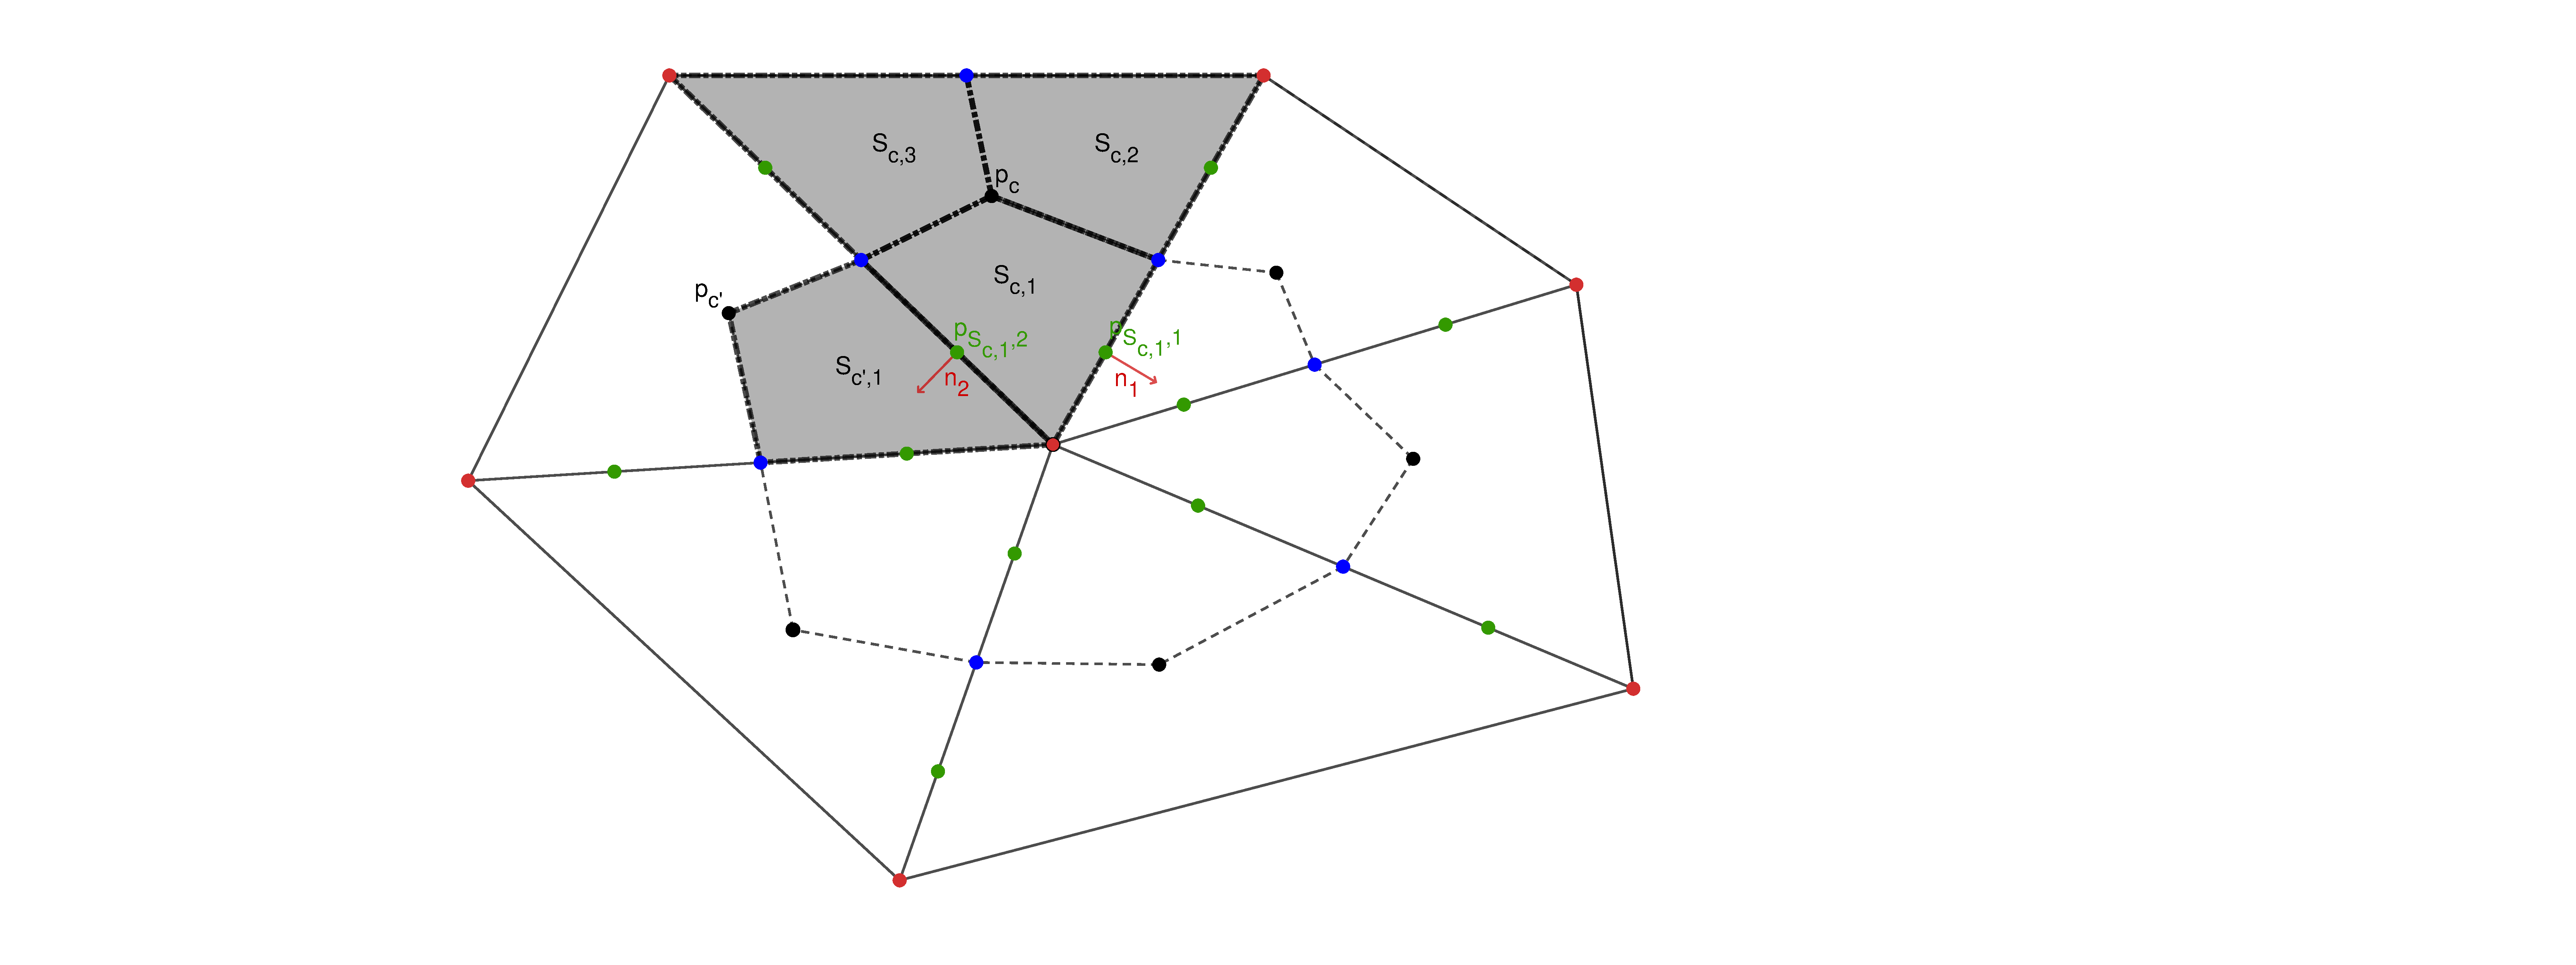
\includegraphics[scale=0.2]{Figure/MPFAPolymac1.pdf}
\caption{Scheme of the MPFA method for a triangular mesh \cite{Bacq}.}
\label{MPFA}
\end{figure}

For a face $f$ of vertex $i$ and $j$, shared by cells $c$ and $c'$, the \textbf{stability condition} of the MPFA method reads:
\begin{equation}
    \forall (k,l) \in \{i,j\}, \ \forall (\tilde{c},\hat{c})\in \{c,c' \}, \ G_{S_{\tilde{c},k}} \cdot G_{S_{\hat{c},l}} \geq 0 \label{MPFA_stability_cdt}
\end{equation}

Some remarks:
{
\it
\begin{itemize} 
    \item  Due to large stencil of the MPFA scheme induced by the elimination of the auxiliary unknows, PolyMAC\_P0 tends to be more costly when using tetrahedron grids rather than hexahedron grids.
    \item  On the boundary of the domain, only one auxiliary quantity is constructed by face when no Dirichlet or Neumann are imposed. 
\end{itemize}
}

\subsection{PolyMAC\textunderscore{}P0-P1NC}
The PolyMAC\_P0-P1NC discretisation aims at reducing some stability issues of PolyMAC\_P0. It uses an Hybrid Finite Volume method described in \cite{eymard2007} in the case of a diffusion problem. Moreover, as in the first PolyMAC discretisation, the vorticity $\omega = \nabla \wedge u$ is introduced. We remind that no source terms are implemented and no validation have been made for this scheme. We do not recommend to use this scheme for most cases.

\section{PolyVEF\textunderscore{}P0\label{sec:polyvef}}
The PolyVEF\_P0 discretisation method is different from the PolyMAC family. Indeed, it is an extension to arbitrary polyhedron of the Crouzeix-Raviart Finite Element Method named VEF in \texttt{TRUST}/\texttt{TrioCFD}, hence the name PolyVEF. In this case, scalar quantities are stored at the cell and at the vertexes. However, the entire velocity vector is stored at the face as described in Figure~\ref{PolyVEF}. As in PolyMAC\_P0, the gradient is reconstructed by using MPFA methods. 
However, time schemes ICE and SETS are not sufficient for using PolyVEF\_P0. We remind that no validation have been made for this scheme and that it is not available in the TRUST environment. We do not recommend to use this scheme for most cases.

\section{VDF\label{sec:vdf}}
This discretisation method is designed to be compatible with conforming meshes composed of hexahedral elements. It is a conservative Finite Volume scheme of MAC \cite{harlow1965numerical} type.
All scalars are stored at the center of each control volume when the velocity field which is defined on a staggered mesh. It is summarized on Figure~\ref{VDF}. It must be emphasised that a hexahedral mesh is not considered being a cartesian mesh. In practise, hexahedral grids are not always cartesian.

This discretisation allows 2D axi-symetrical configurations. It can be activated using the keyword \texttt{bidim\_axi}.

\section{Boundary conditions\label{sec:bounda-condi}}
An object called a boundary condition is used to define, for a given equation, the conditions to be applied on a domain's boundary. Each boundary condition object contains a reference to the \texttt{Domain\_Cl\_dis\_base} object to which it belongs. Each object also contains a \texttt{Champ\_front} object containing the values to be imposed on the boundary.
The main \texttt{Champ\_front} used are summarized in the following table \ref{Champfront}. 

\begin{table}[!ht]
    \centering
       \begin{tabular}{c c  c }
        \toprule
        Keyword & Steady & Uniform \\
        \midrule
        \rowcolor[gray]{0.9} \texttt{champ_front_uniforme} & \checkmark & \checkmark  \\
        \texttt{champ_front_fonc_xyz} &  \checkmark & \xmark \\
        \rowcolor[gray]{0.9} \texttt{champ_front_fonc_t} & \xmark &  \checkmark \\
        \texttt{champ_front_fonc_txyz} & \xmark & \xmark \\
        \bottomrule
    \end{tabular}
    \caption{Main Champ_front for boundary conditions.}
    \label{Champfront}
\end{table}

In multiphase problems \texttt{champ\_front\_composite} can be used to associate different boundary conditions to each phase. For example:
\begin{lstlisting}
champ_front_composite 2
{
    champ_front_uniforme 3 0 0 1
    champ_front_uniforme 3 0 0 1
}
\end{lstlisting}
A special \texttt{Champ\_Front\_MUSIG} associated with \texttt{Milieu_MUSIG} can be used to give boundary conditions to each phase. For example: 
\begin{lstlisting}
Champ_Front_MUSIG {
    nbPhases 1 Champ_Front_Uniforme 1 0.03 # Gas 0 #
    nbPhases 1 Champ_Front_Uniforme 1 0.04 # Gas 1 #
    nbPhases 1 Champ_Front_Uniforme 1 0.05 # Gas 2 #
    nbPhases 1 Champ_Front_Uniforme 1 0.07 # Gas 3 #
    nbPhases 1 Champ_Front_Uniforme 1 0.03 # Liquid 0 #
    nbPhases 1 Champ_Front_Uniforme 1 0.05 # Liquid 1 #
    nbPhases 1 Champ_Front_Uniforme 1 0.07 # Liquid 2 #
    nbPhases 1 Champ_Front_Uniforme 1 0.09 # Liquid 3 #
    nbPhases 1 Champ_Front_Uniforme 1 0.11 # Liquid 4 #
    nbPhases 1 Champ_Front_Uniforme 1 0.13 # Liquid 5 #
    nbPhases 1 Champ_Front_Uniforme 1 0.15 # Liquid 6 #
    nbPhases 1 Champ_Front_Uniforme 1 0.17 # Liquid 7 #
}
\end{lstlisting}
We present in the following tables the main boundary conditions available for the mass (Table~\ref{BCmass}), momentum (Table~\ref{BCmomentum}) and energy equations (Table~\ref{BCenergy}).

\begin{table}[!ht]
    \centering
    \begin{tabular}{ c c }
        \toprule
        Condition & Keyword \\
        \midrule
        \rowcolor[gray]{0.9} Dirichlet & \texttt{frontiere\_ouverte} \\
        Wall & \texttt{paroi} \\
        \rowcolor[gray]{0.9} Symmetry & \texttt{symetrie} \\
        Mass flux & \texttt{Neumann\_paroi} \\
        \bottomrule
    \end{tabular}
    \caption{Boundary conditions for mass equation.}\label{BCmass}
\end{table}

\begin{table}[!ht]
    \centering
    \begin{tabular}{ c c }
        \toprule
        Condition & Keyword \\
        \midrule
        \rowcolor[gray]{0.9} Dirichlet & \texttt{frontiere\_ouverte} \\
        Dirichlet on velocity inlet & \texttt{frontiere\_ouverte\_vitesse\_imposee} \\
        \rowcolor[gray]{0.9} Dirichlet on velocity of open boundary &  \texttt{frontiere\_ouverte\_vitesse\_imposee\_sortie} \\
        Dirichlet on pressure of open boundary & \texttt{frontiere\_ouverte\_pression\_imposee} \\
        \rowcolor[gray]{0.9} Dirichlet on tangential velocity & \texttt{paroi\_defilante} \\
        Wall function & \texttt{Paroi\_frottante\_loi} \\
        \rowcolor[gray]{0.9} Symmetry & \texttt{symetrie} \\
        Adhesion to the wall & \texttt{paroi\_fixe} \\  
        \bottomrule
    \end{tabular}
    \caption{Boundary conditions for momentum equation.}\label{BCmomentum}
\end{table}

\begin{table}[!ht]
    \centering
    \begin{tabular}{ c c }  
       \toprule
        Condition & Keyword \\
        \midrule
        \rowcolor[gray]{0.9} Dirichlet on temperature & \texttt{frontiere\_ouverte} \\
        Dirichlet on temperature for wall & \texttt{paroi\_temperature\_imposee} \\
        \rowcolor[gray]{0.9} Adiabatic wall & \texttt{paroi\_adiabatique} \\
        Wall flux & \texttt{paroi\_flux\_impose} \\
        \rowcolor[gray]{0.9} Symmetry & \texttt{symetrie} \\
        Zero diffusion flux & \texttt{frontiere\_ouverte\_temperature\_imposee} \\
        \bottomrule
    \end{tabular}
        \caption{Boundary conditions for energy equation.}
    \label{BCenergy}

\end{table}

Remark : \textit{ No periodic boundary conditions or mixed conditions are implemented. We observe that the second one could be easier to implement.}

\cleardoublepage

% Physics
\chapter{Two-fluid physical modeling\label{sec:phyical_modeling}}

This chapter details the physical models for the Two-fluid approach. First, the definition of fluid properties is defined using two methods, through the dataset (section~\ref{sec:fluid_properties} and through an external software (section~\ref{sec:fluid-prop-ext}). Then the interfacial forces are described in section~\ref{sec:interfa-forces}. Some particular source terms for the momentum (section~\ref{sec:analytical}) and the mass equations (section~\ref{sec:injection}). The management of the dispersed phase diameter is described in section~\ref{sec:diam-mgmt}.

%%%
\section{Fluid proprieties\label{sec:fluid_properties}}
\subsection{Basic proprieties of fluid}
The domain used for the different phases must be defined by a medium characterized by one or more fluid subdomains of different properties. This composite environment is defined by \texttt{Milieu\_composite}.\\
The models aims to give the basic proprieties of fluids such as :
\begin{itemize}
    \item[\small \textcolor{blue}{\ding{109}}] Kinematic viscosity $\mu$
    \item[\small \textcolor{blue}{\ding{109}}] Density $\rho$
    \item[\small \textcolor{blue}{\ding{109}}] Thermal diffusivity $\alpha$
    \item[\small \textcolor{blue}{\ding{109}}] Conductivity $\lambda$
    \item[\small \textcolor{blue}{\ding{109}}] Calorific capacity $Cp$
    \item[\small \textcolor{blue}{\ding{109}}] Thermal dilatation coefficient $\beta_{co}$
\end{itemize}
The model is implemented in \texttt{Fluide_reel_base} as
\begin{lstlisting}[language=c++]
void Fluide_reel_base::set_param(Param& param)
{
  param.ajouter("T_ref", &T_ref_);
  param.ajouter("P_ref", &P_ref_);
  set_additional_params(param);
}
\end{lstlisting}
The fluid proprieties operator must fill following tabs :
\begin{itemize}
   \item[\small \textcolor{blue}{\ding{109}}] \texttt{rho\textunderscore} density
   \item[\small \textcolor{blue}{\ding{109}}] \texttt{dP\textunderscore rho\textunderscore} density derivative regarding pressure
   \item[\small \textcolor{blue}{\ding{109}}] \texttt{dT\textunderscore rho\textunderscore} density derivative regarding temperature
   \item[\small \textcolor{blue}{\ding{109}}] \texttt{h\textunderscore} enthalpy
   \item[\small \textcolor{blue}{\ding{109}}] \texttt{dP\textunderscore h\textunderscore} enthalpy derivative regarding pressure
   \item[\small \textcolor{blue}{\ding{109}}] \texttt{dT\textunderscore h\textunderscore} enthalpy derivative regarding temperature
   \item[\small \textcolor{blue}{\ding{109}}] \texttt{cp\textunderscore} heat capacity
   \item[\small \textcolor{blue}{\ding{109}}] \texttt{beta\textunderscore} thermal dilatation coefficient
   \item[\small \textcolor{blue}{\ding{109}}] \texttt{mu\textunderscore} kinematic viscosity
   \item[\small \textcolor{blue}{\ding{109}}] \texttt{lambda\textunderscore} conductivity
\end{itemize}

%%%
\subsubsection{Non-compressible fluid}
The model is implemented in \texttt{Fluide\_Incompressible} (from TRUST incompressible) :
\begin{lstlisting}[language=c++]
void Fluide_Incompressible::set_param(Param& param)
{
  Fluide_base::set_param(param);
  //La lecture de rho est rendue obligatoire ici
  param.supprimer("rho");
  param.ajouter("rho",&rho,Param::REQUIRED);
}
\end{lstlisting}
This class allows to give the proprieties previously introduced (or are set to $0$) but with a density that is mandatory. Let's notice that here neither the density nor the specific heat can be a \texttt{Champ_Uniforme}.

%%%
\subsubsection{Sodium gas}
The model is implemented in \texttt{Fluide\_sodium\_gaz} :
\begin{lstlisting}[language=c++]
void Fluide_sodium_gaz::set_param(Param& param)
\end{lstlisting}
The model implemented reads \texttt{Lois\_sodium.h} and writes:
\begin{itemize}
   \item[\small \textcolor{blue}{\ding{109}}] { "temperature", { 371 - 273.15, 2503.7 - 273.15 } }, //Tri-critical point temperature { "pression", { 4.127e-6, 260e5 } };                // Associated pressure
\end{itemize}

%%%
\subsubsection{Sodium liquid}
The model is implemented in \texttt{Fluide\_sodium\_liquide}:
\begin{lstlisting}[language=c++]
void Fluide_sodium_liquide::set_param(Param& param)
\end{lstlisting}
The model implemented reads \texttt{Lois\_sodium.h} and writes:
\begin{itemize}
  \item[\small \textcolor{blue}{\ding{109}}] { "temperature", { 371 - 273.15, 2503.7 - 273.15 } }; //de la temperature de solidification au pt tricritique
\end{itemize}

%%%
\subsubsection{Stiffened gas}
The model is implemented in \texttt{Fluide\_stiffened\_gas}:
\begin{lstlisting}[language=c++]
void Fluide_stiffened_gas::set_param(Param& param)
{
  Fluide_reel_base::readOn(is);
  if (Cv_ == -1.) Cv_ = R_ / (gamma_ - 1.0);
  return is;
}
void Fluide_stiffened_gas::set_param(Param& param)
{
  Fluide_reel_base::set_param(param);
  param.ajouter("gamma",&gamma_); // Heat ratio
  param.ajouter("pinf",&pinf_); // Reference pressure in law
  param.ajouter("mu",&mu__); // viscosity
  param.ajouter("lambda",&lambda__); // conductivity
  param.ajouter("Cv",&Cv_); // heat capacity
  param.ajouter("q",&q_);
  param.ajouter("q_prim",&q_prim_);
}
\end{lstlisting}
The model implemented is:
\begin{itemize}
  \item[\small \textcolor{blue}{\ding{109}}] \texttt{rho\textunderscore} $=\frac{p+\texttt{pinf\textunderscore}}{\left(\texttt{gamma\textunderscore} -1.0\right)\left(T+\num{273.15}\right)\texttt{Cv\textunderscore}}$, the density
  \item[\small \textcolor{blue}{\ding{109}}] \texttt{dP\textunderscore rho\textunderscore} $=\frac{1.0}{\left(\texttt{gamma\textunderscore} -1.0\right)\left(T+\num{273.15}\right)\left(\texttt{Cv\textunderscore} \right)}$, the density derivative regarding pressure
  \item[\small \textcolor{blue}{\ding{109}}] \texttt{dT\textunderscore rho\textunderscore}$ =-\frac{p+\texttt{pinf\textunderscore}}{\left(\texttt{gamma\textunderscore} - 1.0\right)\left(T+\num{273.15}\right)^2\texttt{Cv\textunderscore}}$, the density derivative regarding temperature
  \item[\small \textcolor{blue}{\ding{109}}] \texttt{h\textunderscore } $=\texttt{ gamma\textunderscore Cv\textunderscore}\left(T+\num{273.15}\right)+\texttt{q\textunderscore}$, the enthalpy
  \item[\small \textcolor{blue}{\ding{109}}] \texttt{dP\textunderscore h\textunderscore} $=0.$, the enthalpy derivative regarding pressure
  \item[\small \textcolor{blue}{\ding{109}}] \texttt{dT\textunderscore h\textunderscore}$ = \texttt{cp\textunderscore} \left(T,P\right)$, the enthalpy derivative regarding temperature
  \item[\small \textcolor{blue}{\ding{109}}] \texttt{cp\textunderscore} $ = \texttt{gamma\textunderscore Cv\textunderscore}$, the heat capacity
  \item[\small \textcolor{blue}{\ding{109}}] \texttt{beta\textunderscore}$ = \frac{1.0}{T+\num{273.15}}$
  \item[\small \textcolor{blue}{\ding{109}}] \texttt{mu\textunderscore}$ = \texttt{mu\textunderscore \textunderscore}$
  \item[\small \textcolor{blue}{\ding{109}}] \texttt{lambda\textunderscore}$ = \texttt{lambda\textunderscore \textunderscore}$
\end{itemize}

%%%
\subsubsection{R12_C1 and Eau_c3}
The models are implemented in \texttt{Fluide\_R12\_c1\_liquide}, \texttt{Fluide\_R12\_c1\_gaz}, \texttt{Fluide\_eau\_c3\_liquide} and \texttt{Fluide\_eau\_c3\_gaz}. The low boiling of refrigerant R12 (dichlorodifluoromethane) mimics Pressurized water reactor dimensionless numbers. Those values are available in Cathare code.
For example, in \textcite{KREPPER20113851}, one can find : \\
\begin{center}
\begin{tabular}{c c c }
\toprule
Fluid & Water & R12 \\ \midrule
\rowcolor[gray]{0.9} Pressure [bar] & $155$ & $26$ \\
$T_{sat}$ [\textdegree C] &  $344.9$ &  $86.5$ \\
\rowcolor[gray]{0.9} $\rho_{liquid}$ [kg/m3] &  $594.4$ & $1019.3$ \\
$Cp_{liquid}$ [kJ/kg] &  $8.950$ & $1.413$ \\
\rowcolor[gray]{0.9} $\lambda_{liquid}$ [W/m/K] & $0.472$ & $0.0458$ \\
$\mu_{liquid}$ [W/m/K] & $6.82 \times 10^{-5}$ & $9.23 \times 10^{-5}$ \\
\rowcolor[gray]{0.9} $\rho_{steam}$ [kg/m3] & $101.9$ & $170.7$ \\
$Cp_{steam}$ [kJ/kg] & $14.0$ & $1.281$\\
\rowcolor[gray]{0.9} $\lambda_{steam}$ [W/m/K] &  $0.126$ &  $0.0175$\\
$\mu_{steam}$ [W/m/K] & $2.30 \times 10^{-5}$ & $1.57 \times 10^{-5} $ \\
\rowcolor[gray]{0.9} $\sigma$ [J/m2] & $4.65 \times 10^{-3}$ & $1.80 \times 10^{-3}$ \\
$L_{vap}$ [kJ/kg] & $966.2$ & $86.48$ \\ \bottomrule
\end{tabular}
\end{center}

%%%
\subsubsection{MUSIG fluid and medium}
In homogeneous MUlti-SIze Group (MUSIG), a distribution of bubbles or droplets between $r_{min}$ and $r_{max}$ is characterized by a statistical law (linear, exponential or log) and its discretization in $n$ sub groups with the same velocity, as depicted in Figures \ref{msgdis} from \textcite{cheung}.
\begin{figure}[!ht]
    \centering
    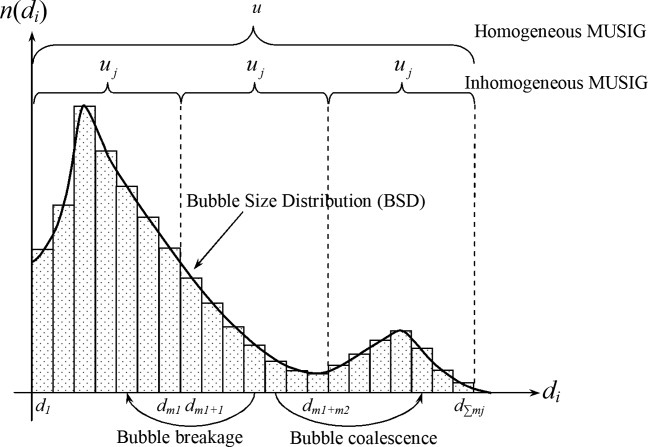
\includegraphics[scale =0.8]{Figure/musigdistri.jpg}
    \caption{Schema of the standard MUSIG and i-MUSIG models. In MUSIG, all size groups move with the same velocity field, whereas i-MUSIG displays an arbitrary number of velocity groups.}
    \label{msgdis}
\end{figure}
All bubbles from sub groups share the same velocity as the velocity of the mean Sauter diameter of the distribution $D_{sm}$. Thus, they share the same common total void fraction equation (mass), velocity (momentum equation) and temperature, allowing to compute only one common set of equations (mass, momentum and energy) with new source terms linked to the changes in the distribution (dilatability, coalescence, break-up).\\
The model is implemented in \texttt{Fluide\_MUSIG} and \texttt{Milieu\_MUSIG} :
\begin{lstlisting}[language=c++]
void Fluide_MUSIG::set_param(Param& param)
{
if(Motcle(mot) == "NBPHASES")
if (Motcle(mot) == "RMIN")
if (Motcle(mot) == "RMAX")
if(Motcle(mot) == "DIAMETRES" || Motcle(mot) == "DIAMETERS")
if (Motcle(mot) == "LIN")
{
    repartionType=0;
}
if (Motcle(mot) == "EXP")
{
    repartionType=1;
}
if (Motcle(mot) == "LOG")
{
    repartionType=2;
}
}
\end{lstlisting}
Default value : $\texttt{nbSubPhases\_} = -1$, $\texttt{rMin}=-1$, $r\texttt{Max}=-1$.\\
Example of data set to perform MUSIG computation :
\begin{lstlisting}[language=c++]
Milieu_MUSIG
{
    gaz_helium FLUIDE_MUSIG
    {
        fluide StiffenedGas { gamma 1.4 pinf 0.0 }
        nbPhases 4
        diametres { rmin 0.01 rmax 0.1 lin }
    }
    liquide_sodium FLUIDE_MUSIG
    {
        fluide StiffenedGas { gamma 4.4 pinf 6e8 }
        nbPhases 8
    }
}
\end{lstlisting}

%%%
\subsection{Interfacial proprieties}
The liquid-gas interface can be characterized by the surface tension $\sigma$.
The model is implemented in \texttt{Interface\_base} as
\begin{lstlisting}[language=c++]
void Interface_base::set_param(Param& param)
{
  Param param(que_suis_je());
  set_param(param);
  param.lire_avec_accolades_depuis(is);
  return is;
}
\end{lstlisting}
Default values : \texttt{sigma\textunderscore \textunderscore} $= -1.$\\
The interfacial propriety operator must fill \texttt{sigma\textunderscore}.

%%%
\subsubsection{Constant surface tension}
The model is implemented in \texttt{Interface\textunderscore sigma\textunderscore constant} :
\begin{lstlisting}[language=c++]
void sigma_(const SpanD T, const SpanD P, SpanD res, int ncomp = 1, int ind = 0) const override
  {
    for (int i =0; i < (int)P.size(); i++)
      res[i * ncomp + ind] = sigma__;
  }
\end{lstlisting}

%%%
\subsection{Saturation proprieties}
The model aims to give the thermal proprieties at saturation conditions. This class inherits from \texttt{Interface}.
The model is implemented in \texttt{Saturation\textunderscore base} as
\begin{lstlisting}[language=c++]
void Saturation_base::set_param(Param& param)
{
  Interface_base::set_param(param);
  param.ajouter("P_ref", &P_ref_);
  param.ajouter("T_ref", &T_ref_);
}
\end{lstlisting}
The saturation proprieties operator must fill following tabs :
\begin{itemize}
   \item[\small \textcolor{blue}{\ding{109}}] \texttt{Tsat}: saturation temperature
   \item[\small \textcolor{blue}{\ding{109}}] \texttt{dP\_Tsat}: saturation temperature derivative regarding pressure
   \item[\small \textcolor{blue}{\ding{109}}] \texttt{Psat}: saturation pressure
   \item[\small \textcolor{blue}{\ding{109}}] \texttt{dT\_ Psat}: saturation pressure derivative regarding temperature
   \item[\small \textcolor{blue}{\ding{109}}] \texttt{Lvap}: phase change enthalpy
   \item[\small \textcolor{blue}{\ding{109}}] \texttt{dP\_Lvap}: phase change enthalpy regarding pressure
   \item[\small \textcolor{blue}{\ding{109}}] \texttt{Hls}: enthalpy of liquid phase at saturation
   \item[\small \textcolor{blue}{\ding{109}}] \texttt{dP\_Hls}: derivative of enthalpy of liquid phase at saturation regarding pressure
   \item[\small \textcolor{blue}{\ding{109}}] \texttt{Hvs}: enthalpy of steam phase at saturation
   \item[\small \textcolor{blue}{\ding{109}}] \texttt{dP\_Hvs}: derivative of enthalpy of steam phase at saturation regarding pressure
\end{itemize}

{\color{red} Warning}:  We suppose that we have a unique pressure field to compute it.

\subsubsection{Constant saturation proprieties}
The model is implemented in \texttt{Saturation\_constant}:
\begin{lstlisting}[language=c++]
void Saturation_constant::set_param(Param& param)
{
  Param param(que_suis_je());
  param.ajouter("Tsat", &tsat_,Param::REQUIRED); // Temperature at saturation
  param.ajouter("Psat", &psat_,Param::REQUIRED); //Pressure at saturation
  param.ajouter("Lvap", &lvap_); // Phase change enthalpy
  param.ajouter("Hlsat", &hls_); // Enthalpy of liquid phase at saturation
  param.ajouter("Hvsat", &hvs_); // Enthalpy of steam phase at saturation
  param.ajouter("tension_superficielle", &sigma__); // Surface tension
  param.lire_avec_accolades_depuis(is);
  // verifications hlsat/hvsat/lvap
  const int i = (lvap_ > 0) + (hls_ > 0) + (hvs_ > 0);
  if (i != 2) Process::exit(que_suis_je() + " Please give 2 properties among {Lvap, Hlsat, Hvsat}");
  if (lvap_ > 0 && hls_ > 0) hvs_ = hls_ + lvap_;
  else if (lvap_ > 0 && hvs_ > 0) hls_ = hvs_ - lvap_;
  else if (hls_ > 0 && hvs_ > 0) lvap_ = hvs_ - hls_;
  else Process::exit(que_suis_je() + "bad parameters");
  return is;
}
\end{lstlisting}
The model implemented is:
\begin{itemize}
   \item[\small \textcolor{blue}{\ding{109}}] $T_{sat} = \texttt{tsat\_}$
   \item[\small \textcolor{blue}{\ding{109}}] $\frac{D T_{sat}}{Dp} = 0$
   \item[\small \textcolor{blue}{\ding{109}}] $P_{sat} = \texttt{psat\_}$
   \item[\small \textcolor{blue}{\ding{109}}] $\frac{D p_{sat}}{DT} =0$
   \item[\small \textcolor{blue}{\ding{109}}] $L_{vap} = \texttt{lvap\_}$
   \item[\small \textcolor{blue}{\ding{109}}] $\frac{D L_{vap}}{Dp} = 0$
   \item[\small \textcolor{blue}{\ding{109}}] $H_{ls} = \texttt{hls_\_}$
   \item[\small \textcolor{blue}{\ding{109}}] $\frac{D H_{ls}}{Dp} = 0$
   \item[\small \textcolor{blue}{\ding{109}}] $H_{vs} = \texttt{hvs_\_}$
   \item[\small \textcolor{blue}{\ding{109}}] $\frac{D H_{vs}}{Dp} = 0$
   \item[\small \textcolor{blue}{\ding{109}}] $\texttt{sigma\_} =\texttt{sigma\_\_}$
\end{itemize}

\subsubsection{Sodium saturation proprieties}
The model is implemented in Saturation_sodium :
\begin{lstlisting}[language=c++]
void Saturation_sodium::set_param(Param& param)
{
return Saturation_base::readOn(is);
}
\end{lstlisting}

%%%
\subsubsection{R12_C1 and Eau_c3}
The models are implemented in \texttt{Fluide\_R12\_c1\_liquide}, \texttt{Fluide\_R12\_c1\_gaz}, \texttt{Fluide\_eau\_c3\_liquide} and \texttt{Fluide\_eau\_c3\_gaz}. The low boiling of refrigerant R12 (dichlorodifluoromethane) mimics Pressurized water reactor dimensionless numbers. Those values are available in Cathare code.\\

%%%
\section{Fluid proprieties from external software\label{sec:fluid-prop-ext}}
In this section, the management of fluid properties through an external software is described. One can use EOS, the CEA-EDF software for state equation management (section xx), or CoolProp, an open-source alternative. Both EOS and CoolProp can call the NIST state equation software named Refprop. EOS can use a user-defined state equation through a plugin. CoolProp provides free state equations for a selected list of fluids\footnote{Available here \href{http://www.coolprop.org/fluid_properties/index.html}{http://www.coolprop.org/fluid_properties/index.html}}.

\subsection{Basic proprieties of fluid}
The generic table of proprieties from external software is implemented in \texttt{Fluide\_generique\_TPPI\_base} :
\begin{lstlisting}[language=c++]
void Fluide_generique_TPPI_base::set_param(Param& param)
#
if (tmax_ < -100. )
  return Fluide_reel_base::unknown_range();
return { { "temperature", { tmin_ - 273.15, tmax_ - 273.15 } }, { "pression", { pmin_, pmax_ } } };
}
\end{lstlisting}
Default values : $tmin\_ = -123.$, $tmax\_ = -123.$, $pmin\_ = -123.$, $pmax\_ = -123.$
\begin{itemize}
   \item[\small \textcolor{blue}{\ding{109}}] $\texttt{rho\_}$ density
   \item[\small \textcolor{blue}{\ding{109}}] $\texttt{dP\_rho\_ }$ density derivative regarding pressure
   \item[\small \textcolor{blue}{\ding{109}}] $\texttt{dT\_rho\_}$ density derivative regarding temperature
   \item[\small \textcolor{blue}{\ding{109}}] $\texttt{h\_}$ enthalpy
   \item[\small \textcolor{blue}{\ding{109}}] $\texttt{dP\_h\_}$ enthalpy derivative regarding pressure
   \item[\small \textcolor{blue}{\ding{109}}] $\texttt{dT\_h\_}$ enthalpy derivative regarding temperature
   \item[\small \textcolor{blue}{\ding{109}}] $\texttt{cp\_}$ heat capacity
   \item[\small \textcolor{blue}{\ding{109}}] $\texttt{beta\_}$ thermal dilatation coefficient
   \item[\small \textcolor{blue}{\ding{109}}] $\texttt{mu\_}$ kinematic viscosity
   \item[\small \textcolor{blue}{\ding{109}}] $\texttt{lambda\_}$ conductivity
\end{itemize}

%%%
\subsubsection{CoolProp}
The model is implemented in \texttt{Fluide\_generique\_CoolProp}:
\begin{lstlisting}[language=c++]
void Fluide_generique_CoolProp::set_param(Param& param)
{
param.ajouter("model|modele", &model_name_, Param::REQUIRED);
param.ajouter("fluid|fluide", &fluid_name_, Param::REQUIRED);
TPPI_ = std::make_shared<EOS_to_TRUST_generique>();
TPPI_->set_fluide_generique(model_name_, fluid_name_);
TPPI_->desactivate_handler(false); // throw on error

if (model_name_ == "CATHARE2" || model_name_ == "EOS_CATHARE2")
{
      tmin_ = TPPI_->tppi_get_T_min();
      tmax_ = TPPI_->tppi_get_T_max();
      pmin_ = TPPI_->tppi_get_p_min();
      pmax_ = TPPI_->tppi_get_p_max();
}
}
\end{lstlisting}
Validity domain for Cathare tables with $\texttt{tmin\_}$, $\texttt{tmax\_}$, $\texttt{pmin\_}$, $\texttt{pmax\_}$.\\
Accessible at \href{http://www.coolprop.org/v4/index.html}{http://www.coolprop.org/v4/index.html}.

%%%
\subsubsection{EOS}
The model is implemented in \texttt{Fluide\_generique\_EOS} :
\begin{lstlisting}[language=c++]
void Fluide_generique_EOS::set_param(Param& param)
{
param.ajouter("model|modele", &model_name_, Param::REQUIRED);
param.ajouter("fluid|fluide", &fluid_name_, Param::REQUIRED);
param.ajouter("phase", &phase_, Param::OPTIONAL); // optional : liquid or vapor. PI : specify the phase it is really useful (better perf for coolprop) !
if (model_name_ == "REFPROP") TPPI_->set_path_refprop();
  tmin_ = TPPI_->tppi_get_T_min();
  tmax_ = TPPI_->tppi_get_T_max();
  pmin_ = TPPI_->tppi_get_p_min();
  pmax_ = TPPI_->tppi_get_p_max();
}
\end{lstlisting}
Validity domain for Refprop tables with $\texttt{tmin\_}$, $\texttt{tmax\_}$, $\texttt{pmin\_}$, $\texttt{pmax\_}$.\\ Availability of 147 pure fluids, 5 pseudo-pure fluids (such as air), and mixtures with up to 20 components. Accessible at \href{https://www.nist.gov/srd/refprop}{https://www.nist.gov/srd/refprop}.

For instance, a boiling flow using \texttt{refprop10} must be specified as
\begin{lstlisting}[language=c++]
liquide_eau Fluide_generique_EOS { model refprop10 fluid waterliquid }
gaz_eau Fluide_generique_EOS { model refprop10 fluid watervapor }
\end{lstlisting}

%%%
\subsection{Saturation proprieties}
The generic table of proprieties from external software is implemented in \texttt{Saturation\_generique\_TPPI\_base} :
\begin{lstlisting}[language=c++]
void Saturation_generique_TPPI_base::set_param(Param& param)
\end{lstlisting}
The saturation proprieties operator must fill following tabs :
\begin{itemize}
   \item[\small \textcolor{blue}{\ding{109}}] $\texttt{Tsat}$ saturation temperature
   \item[\small \textcolor{blue}{\ding{109}}] $\texttt{dP\_Tsat}$ saturation temperature derivative regarding pressure
   \item[\small \textcolor{blue}{\ding{109}}] $\texttt{Psat}$ saturation pressure
   \item[\small \textcolor{blue}{\ding{109}}] $\texttt{dT\_Psat}$ saturation pressure derivative regarding temperature
   \item[\small \textcolor{blue}{\ding{109}}] $\texttt{Lvap}$ phase change enthalpy
   \item[\small \textcolor{blue}{\ding{109}}] $\texttt{dP\_Lvap}$ phase change enthalpy regarding pressure
   \item[\small \textcolor{blue}{\ding{109}}] $\texttt{Hls}$ enthalpy of liquid phase at saturation
   \item[\small \textcolor{blue}{\ding{109}}] $\texttt{dP\_Hls}$ derivative of enthalpy of liquid phase at saturation regarding pressure
   \item[\small \textcolor{blue}{\ding{109}}] $\texttt{Hvs}$ enthalpy of steam phase at saturation
   \item[\small \textcolor{blue}{\ding{109}}] $\texttt{dP\_Hvs}$ derivative of enthalpy of steam phase at saturation regarding pressure
\end{itemize}


\subsubsection{CoolProp}
The model is implemented in \texttt{Fluide\_generique\_CoolProp} :
\begin{lstlisting}[language=c++]
void Fluide_generique_CoolProp::set_param(Param& param)
{
if (model_name_ == "REFPROP") TPPI_->set_path_refprop();
param.ajouter("model|modele", &model_name_, Param::REQUIRED);
param.ajouter("fluid|fluide", &fluid_name_, Param::REQUIRED);
param.ajouter("phase", &phase_, Param::OPTIONAL); // optional : liquid or vapor. PI : specify the phase it is really useful (better perf for coolprop) !
param.ajouter("sigma_mano", &sigma_mano_, Param::OPTIONAL); // optional : because of issues when we call surface tension in TTSE in coolprop ! Try without and if calculation doesn't pass, input sigma
}
\end{lstlisting}
Default value : $\texttt{sigma\_mano\_}=-1.$

\subsubsection{EOS}
The model is implemented in \texttt{Fluide\_generique\_CoolProp} :
\begin{lstlisting}[language=c++]
void Fluide_generique_CoolProp::set_param(Param& param)
{
TPPI_ = std::make_shared<EOS_to_TRUST_Sat_generique>();
param.ajouter("model|modele", &model_name_, Param::REQUIRED);
param.ajouter("fluid|fluide", &fluid_name_, Param::REQUIRED);
param.ajouter("sigma_mano", &sigma_mano_, Param::OPTIONAL); // optional : because of issues when we call surface tension in TTSE in coolprop ! Try without and if calculation doesn't pass, input sigma
}
\end{lstlisting}
Default value : $\texttt{sigma\_mano\_}=-1.$\\
For example :
\begin{lstlisting}[language=c++]
saturation_eau saturation_generique_EOS { model refprop10 fluid waterliquid }
\end{lstlisting}

%%%
\section{Interfacial forces\label{sec:interfa-forces}}
The interfacial forces defined below are source terms that can be added to the momentum equation and represent the mechanical interactions between the phases. Then the equations of motion for each phase velocities are coupled by the interfacial forces.
% Note de travail. Format général :
% \begin{itemize}
%     \item[\small \textcolor{blue}{\ding{109}}] Nom du fichier implémentant le modèle
%     \item[\small \textcolor{blue}{\ding{109}}] Nom de la classe implémentant le modèle
%     \item[\small \textcolor{blue}{\ding{109}}] Le readon de la classe (très beau ce listing) avec les valeurs par défaut
%     \item[\small \textcolor{blue}{\ding{109}}] La formule écrite dans le code
%     \item[\small \textcolor{blue}{\ding{109}}] Le papier de référence s'il existe et des commentaires si elle diffère du papier de réf
%     \item[\small \textcolor{blue}{\ding{109}}] Cas test associé si existant
% \end{itemize}

%%
\subsection{The Drag force}
The general expression of the drag force is:
\begin{equation}
\overrightarrow{F_{l\rightarrow g}^D}= - \frac{3}{4} C_D \frac{\alpha_g\rho_l}{d_b} \norm{\norm{\overrightarrow{u_g}-\overrightarrow{u_l}}} \parent{\overrightarrow{u_g}-\overrightarrow{u_l}}=-f^{D}||\overrightarrow{u_g}-\overrightarrow{u_l}||\left(\overrightarrow{u_g}-\overrightarrow{u_l}\right)
\end{equation}
The force is implemented in :
\begin{lstlisting}[language=c++]
void Source_Frottement_interfacial_base::set_param(Param& param)
{
  Param param(que_suis_je());
  param.ajouter("a_res", &a_res_);
  param.ajouter("dv_min", &dv_min);
  param.ajouter("exp_res", &exp_res);
  param.ajouter("beta", &beta_);
  param.lire_avec_accolades_depuis(is);

  const Pb_Multiphase& pbm = ref_cast(Pb_Multiphase, equation().probleme());
  if (pbm.has_correlation("frottement_interfacial")) correlation_ = pbm.get_correlation("frottement_interfacial"); //correlation fournie par le bloc correlation
  else correlation_.typer_lire(pbm, "frottement_interfacial", is); //sinon -> on la lit
  return is;
}
\end{lstlisting}
Default values : $\texttt{ a\_res\_} = -1.$, $\texttt{dv\_min} = 0.01$, $\texttt{beta\_}= 1.$, $\texttt{exp\_res} = 2$.\\
The interfacial drag operator must fill coeff tab so that :
\begin{itemize}
    \item[\small \textcolor{blue}{\ding{109}}]$\text{coeff}({\color{myteal}k1}, {\color{mydarkorchid}k2}, 0) = f^{D}||\overrightarrow{u_{{\color{myteal}k1}}}-\overrightarrow{u_{{\color{mydarkorchid}k2}}}||;$
    \item[\small \textcolor{blue}{\ding{109}}]$\text{coeff}({\color{myteal}k1}, {\color{mydarkorchid}k2}, 1) = f^{D};$ (it is the derivative of $\text{coeff}({\color{myteal}k1}, {\color{mydarkorchid}k2}, 0)$ with respect to the relative velocity)
    \item[\small \textcolor{blue}{\ding{109}}]$\text{coeff}({\color{mydarkorchid}k2}, {\color{myteal}k1}, 0) = \text{coeff}({\color{myteal}k1}, {\color{mydarkorchid}k2}, 0);$
    \item[\small \textcolor{blue}{\ding{109}}]$\text{coeff}({\color{mydarkorchid}k2}, {\color{myteal}k1}, 1) = \text{coeff}({\color{myteal}k1}, {\color{mydarkorchid}k2}, 1);$
\end{itemize}

\begin{table}[!ht]
\begin{center}
\renewcommand{\arraystretch}{1}
   \begin{tabular}{ c  c  c c }
     \toprule
     Model & Used & Validated & Test case  \\
    \midrule
     \rowcolor[gray]{0.9} Constant & \checkmark & \checkmark (100\%) & TrioCFD/Tube analytique,\\
     \rowcolor[gray]{0.9} \ & \ & \ & Trust/Tube analytique \\
     Composant & \checkmark & \xmark (0\%) &  \ \\
     \rowcolor[gray]{0.9} Ishii Zuber Deformable &\checkmark & \xmark (0\%) & \ \\
     Ishii Zuber &\checkmark & \xmark (0\%) & \ \\
     \rowcolor[gray]{0.9} Tomiyama &\checkmark & \checkmark (100\%) & TrioCFD/CoolProp, \\
     \rowcolor[gray]{0.9} \ & \ & \ & TrioCFD/Gabillet\\
     Weber &\checkmark & \xmark (0\%) & \ \\
     \rowcolor[gray]{0.9} Wallis &\checkmark & \xmark (0\%) & \ \\
     Sonnenburg &\checkmark & \xmark (0\%) & \ \\
     \rowcolor[gray]{0.9} Garnier &\checkmark & \xmark (0\%) & \ \\
     Rusche &\checkmark & \xmark (0\%) & \ \\
     \rowcolor[gray]{0.9} Simmonet & \checkmark & \xmark (0\%) & \ \\
     Zenit &\checkmark & \xmark (0\%) & \ \\
     \bottomrule
   \end{tabular}
 \end{center}
\caption{Availability of drag force models in Trio\textunderscore CMFD.}
\label{dragtable}
\end{table}

\subsubsection{Constant drag coefficient}
The model is implemented in :
\begin{lstlisting}[language=c++]
void Frottement_interfacial_bulles_constant::set_param(Param& param)
{
param.ajouter("coeff_derive", &C_d_, Param::REQUIRED);
param.ajouter("rayon_bulle", &r_bulle_);
}
\end{lstlisting}
Default values : $\texttt{r\_bulles\_}=-1$, $\texttt{C\_d\_}=-123.$.\\
If no rayon\_bulle takes d\_bulles.\\
The model implemented is :
\begin{equation}
   f^{D}=\frac{3}{4}\frac{C_d\alpha_g\rho_l}{d_b}.
\end{equation}

\subsubsection{Composant drag coefficient}
The model is implemented in :
\begin{lstlisting}[language=c++]
void Frottement_interfacial_bulles_composant::set_param(Param& param)
{
param.ajouter("coeff_derive", &C_d_, Param::REQUIRED);
param.ajouter("rayon_bulle", &r_bulle_);
}
\end{lstlisting}
Default values $\texttt{r\_bulle\_}=-100$, $\texttt{C\_d}=-100.$.\\
The model implemented is :
\begin{equation}
   f^{D}_{ij}=\frac{3}{4}\frac{C_d\alpha_i\alpha_j\rho_m}{d_b},
\end{equation}
with $\rho_m=\sum_k \alpha_k \rho_k$ and $i \neq j$.
\subsubsection{Ishii-Zuber : viscous regime}
The model is described in \textcite{IshiiZuber}.\\
The model is implemented in:
\begin{lstlisting}[language=c++]
void Frottement_interfacial_Ishii_Zuber_Deformable::set_param(Param& param)
{
  param.ajouter("beta", &beta_);
  param.ajouter("constante_gravitation", &g_);
}
\end{lstlisting}
Default values : $\texttt{g\_}=9.81$, $\texttt{beta\_}=1.$.\\
The model implemented is :
\begin{equation}
   f^{D}=\frac{1}{2}\alpha_g\rho_l\sqrt{\frac{\left(\rho_l-\rho_g\right)\times{}g}{\sigma}}\frac{1}{\sqrt{max\left(1-\alpha_g,\ 0.001\right)}}.
\end{equation}
If $\alpha_l < \num{1.e-6}$, then $f^D\times{}\alpha_l\times{}\num{1e6}$.

\subsubsection{Ishii-Zuber : viscous regime and particle regime}
The model is also described in \textcite{IshiiZuber}.\\
The model is implemented as :
\begin{lstlisting}[language=c++]
void Frottement_interfacial_Ishii_Zuber::set_param(Param& param)
{
  param.ajouter("beta", &beta_);
  param.ajouter("constante_gravitation", &g_);
}
\end{lstlisting}
Default values $\texttt{g\_}=9.81$, $\texttt{beta\_}=1.$.
The model implemented is :
\begin{equation}
   f^{D}=\frac{3}{4}\frac{\text{max}\parent{\frac{24}{Re_b}\left(1+0.1Re_b^{0.75}\right),\ \frac{2}{3}\sqrt{\frac{\left(\rho_l-\rho_g\right)g d_b^2}{\sigma}}}\beta \alpha_g\rho_l}{d_b },
\end{equation}
with $Re_b=\frac{\rho_l d (u_g-u_l)}{\mu_l}$.
\subsubsection{Tomiyama : contaminated drag coefficient}
The model is described in \textcite{Tomiyama1998}.\\
The model is implemented in :
\begin{lstlisting}[language=c++]
void Frottement_interfacial_Tomiyama::set_param(Param& param)
{
  param.ajouter("beta", &beta_);
  param.ajouter("constante_gravitation", &g_);
  param.ajouter("contamination", &contamination_);
}
\end{lstlisting}
Default values : $\texttt{g\_}=9.81$, $\texttt{beta\_}=1.$, $contamination=0$.\\
The model implemented is :
\begin{equation}
f_D =\frac{3}{4}\frac{\alpha_g\rho_l}{d} \begin{cases} \max(\min(16/Re_b(1+.15Re^{.687}), 48/Re_b), 8Eo/(3+12)) \text{, No contamination (0)}\\
	\max(\min(24/Re_b(1+.15Re_b^{.687}), 72/Re_b), 8Eo/(3Eo+12)) \text{, Slight contamination (1)}\\
	\max(24/Re_b(1+.15Re_b^{.687}), 8Eo/(3Eo+12)) \text{, High contamination (2)} \end{cases}
\end{equation}
with
\begin{itemize}
    \item[\small \textcolor{blue}{\ding{109}}]$Eo = \frac{g(\rho_l-\rho_v)d^2}{\sigma}$,
    \item[\small \textcolor{blue}{\ding{109}}]$Re_b=\frac{\rho_l d_b (u_g-u_l)}{\mu_l}$.
\end{itemize}
If $\alpha_l < \num{1.e-6}$, then $f^D\times{}\alpha_l\times{}\num{1e6}$.\\
This formulation was chosen as shown in \textcite{Sugrue2017}, it yields similar results as other closures and one can adjust the level of contamination.

\subsubsection{Bubble critical diameter (incoming)}
The model is described partially in \textcite{KUO1988547}.\\
The model is implemented in :
\begin{lstlisting}[language=c++]
void Frottement_interfacial_Weber::set_param(Param& param)
{
    param.ajouter("Weber_critique", &We_c);
}
\end{lstlisting}
Default values $We\_ c=8.$.\\
The model implemented is :
\begin{equation}
   f^{D}=\frac{6\alpha_g}{\pi d_b^{*3}}\frac{24}{Re_b}(1+0.1Re_b^{0.75}),
\end{equation}
with $d_b^*= \frac{\sigma}{\rho_l(u_g-u_l)^2}We_c$, $Re_b=\frac{\rho_l d_b^* (u_g-u_l)}{\mu_l}$.\\
{\color{red} Warning} : not homogeneous

\subsubsection{Wallis : annular flow}
The model is described in \textcite{wallis}.\\
The model is implemented in :
\begin{lstlisting}[language=c++]
void Frottement_interfacial_Wallis::set_param(Param& param)
\end{lstlisting}
The model implemented is :
\begin{equation}
   f^{D}=\num{5e-3}\times{}\rho_g\frac{4\sqrt{\alpha_g}}{D_h}\parent{1+300\frac{1-\sqrt{1-\alpha_g}}{2}}
\end{equation}

\subsubsection{Sonnenburg : drift flux ?}
The model is described in .\\
The model is implemented in :
\begin{lstlisting}[language=c++]
void Frottement_interfacial_Sonnenburg::set_param(Param& param)
\end{lstlisting}
The model implemented is :
\begin{equation}
   f^{D}=\rho_l\frac{\alpha_l\alpha_g}{D_h}\Big(\frac{16}{9}(1-\alpha_g^*(1-\frac{9}{16}\sqrt{\frac{\rho_g}{\rho_l}}))\frac{1-\alpha_g^{*40}}{tanh(32\alpha_g^*)}\Big)^2,
\end{equation}
with $\alpha_g^*=min(max(\alpha_g,0.001),0.999)$

\subsubsection{Garnier : bubble swarm correction}
The model is described in \textcite{GARNIER2002811}.\\
The model is implemented in :
\begin{lstlisting}[language=c++]
void Frottement_interfacial_Garnier::set_param(Param& param)
\end{lstlisting}
The model implemented is :
\begin{equation}
   f^{D}_{new}=f^{D}\begin{cases} \alpha_l\times 114.2,\text{ if }\alpha_l< 0.5  \\
          \parent{1-\alpha_g^{1/3}}^{-2},\text{ if not}.
   \end{cases}
\end{equation}
{\color{red} Warning} : Validated for $\alpha_g  < 0.35$, $D_{sm} < 5.5mm$.

\subsubsection{Rusche : swarm correction}
The model is described in \textcite{Rusche}.\\
The model is implemented in :
\begin{lstlisting}[language=c++]
void Frottement_interfacial_Rusche::set_param(Param& param)
\end{lstlisting}
The model implemented is :
\begin{equation}
   f^{D}_{new}=f^{D}\parent{\exp\parent{3.64\alpha_g}+\alpha_g^{0.864}}
\end{equation}
{\color{red} Warning} : Validated for $\alpha_g  < 0.5$.

\subsubsection{Simonnet : bubble swarm correction}
The model is described in \textcite{SIMONNET2007858}.\\
The model is implemented in :
\begin{lstlisting}[language=c++]
void Frottement_interfacial_Simonnet::set_param(Param& param)
\end{lstlisting}
The model implemented is :
\begin{equation}
   f^{D}_{new}=f^{D}\alpha_l\parent{\alpha_l^{25} + \parent{4.8\frac{\alpha_g}{\alpha_l}}^{25}}^{-2/25}
\end{equation}
{\color{red} Warning} : Validated for $\alpha_g  < 0.3$, $D_{sm} < 10 mm$.

\subsubsection{Zenit : bubble swarm correction}
The model is described in \textcite{zenit}.\\
The model is implemented in :
\begin{lstlisting}[language=c++]
void Frottement_interfacial_Zenit::set_param(Param& param)
\end{lstlisting}
The model implemented is :
\begin{equation}
   f^{D}_{new}=f^{D}\frac{\parent{1+3\alpha_g}^2}{\alpha_l^2}
\end{equation}
{\color{red} Warning} : Validated for  $\alpha_g  < 0.18$.

%%
\subsection{The Lift force}
The general expression of the lift force is :
\begin{equation}
	\overrightarrow{F_{l\rightarrow v}^L}
	= -C_L \rho_l \alpha_g \parent{\overrightarrow{u_g} - \overrightarrow{u_l}} \wedge \overrightarrow{u_l}
	= -f^L\parent{\overrightarrow{u_g} - \overrightarrow{u_l}} \wedge \overrightarrow{u_l}
\end{equation}
The force is implemented in :
\begin{lstlisting}[language=c++]
void Source_Portance_interfaciale_base::set_param(Param& param)
{
  Param param(que_suis_je());
  param.ajouter("beta", &beta_);
  param.ajouter("g", &g_);
  param.lire_avec_accolades_depuis(is);

  Pb_Multiphase *pbm = sub_type(Pb_Multiphase, equation().probleme()) ? &ref_cast(Pb_Multiphase, equation().probleme()) : NULL;

  if (!pbm || pbm->nb_phases() == 1) Process::exit(que_suis_je() + " : not needed for single-phase flow!");

  for (int n = 0; n < pbm->nb_phases(); n++) //recherche de n_l, n_g : phase {liquide,gaz}_continu en priorite
    if (pbm->nom_phase(n).debute_par("liquide") && (n_l < 0 || pbm->nom_phase(n).finit_par("continu")))  n_l = n;

  if (n_l < 0) Process::exit(que_suis_je() + " : liquid phase not found!");

  if (pbm->has_correlation("Portance_interfaciale")) correlation_ = pbm->get_correlation("Portance_interfaciale"); //correlation fournie par le bloc correlation
  else correlation_.typer_lire((*pbm), "Portance_interfaciale", is); //sinon -> on la lit

  pbm->creer_champ("vorticite"); // Besoin de vorticite

  return is;
}
\end{lstlisting}
Default values : $\texttt{beta\_} = 1.$, $\texttt{g\_} = 9.81$.\\
The interfacial lift operator must fill out.Cl tab so that :
\begin{itemize}
\item[\small \textcolor{blue}{\ding{109}}]$Cl({\color{myteal}k1}, {\color{mydarkorchid}k2}) = f^L ;$
\item[\small \textcolor{blue}{\ding{109}}]$Cl({\color{mydarkorchid}k2}, {\color{myteal}k1}) = Cl({\color{myteal}k1}, {\color{mydarkorchid}k2});$
\end{itemize}

\begin{table}[!ht]
\begin{center}
\renewcommand{\arraystretch}{1}
   \begin{tabular}{ c  c  c c }
     \toprule
     Model & Used & Validated & Test case  \\
    \midrule
     \rowcolor[gray]{0.9}Constant & \checkmark & \checkmark (100\%) & TrioCFD/Tube analytique,\\
    \rowcolor[gray]{0.9} \ & \ & \ & TrioCFD/CoolProp, \\
    \rowcolor[gray]{0.9} \ & \ & \ & Trust/Tube analytique \\
     Sugrue & \checkmark & \checkmark (100\%) & TrioCFD/CoolProp \\
     \ & \ & \ & TrioCFD/Gabillet \\
     \rowcolor[gray]{0.9} Tomiyama &\checkmark & \xmark (0\%) & \ \\
     \bottomrule
   \end{tabular}
 \end{center}
\caption{Availability of lift force models in Trio\textunderscore CMFD.}
\label{lifttable}
\end{table}

%
\subsubsection{Constant lift coefficient}
The model is implemented in :
\begin{lstlisting}[language=c++]
void Portance_interfaciale_Constante::set_param(Param& param)
{
  param.ajouter("Cl", &Cl_, Param::REQUIRED);
}
\end{lstlisting}
Default values $\texttt{Cl\_}=-123.$\\
The model implemented is :
\begin{equation}
   f^{L} = C_L\rho_l\alpha_g\text{max}\parent{\text{min}\parent{\frac{\alpha_l - 0.05}{0.25},\ 1 },\ 0}
\end{equation}
The void fraction correction is used to damp the lift at too high void fractions.

%
\subsubsection{Sugrue}
The model is described in .\\
The model is implemented in :
\begin{lstlisting}[language=c++]
void Portance_interfaciale_Sugrue::set_param(Param& param)
{
  param.ajouter("constante_gravitation", &g_);
}
\end{lstlisting}
Default values $\texttt{g\_}=9.81$.\\
The model implemented is :
\begin{equation}
   f^{L} = \rho_l\alpha_g \text{max}\parent{1.0155-0.0154\exp\parent{8.0506\alpha_g},\ 0} \times \text{min}\parent{5.0404-5.0781(Wo)^{0.0108},\ 0.03}
\end{equation}
with
\begin{itemize}
    \item[\small \textcolor{blue}{\ding{109}}]the wobbling number $\mathit{Wo}=\text{min}\parent{\frac{k_lEo}{\text{max}\parent{\parent{u_g-u_l}^2,\ \num{1e-8}}},\ 6.}$
    \item[\small \textcolor{blue}{\ding{109}}]the Eotvos number $\mathit{Eo}=\frac{g\parent{\rho_l-\rho_g}d_b^2}{\sigma}$
\end{itemize}.

%
\subsubsection{Tomiyama : lift sign reversal}
The model is described in \textcite{Tomiyama2002}.\\
The model is implemented in :
\begin{lstlisting}[language=c++]
void Portance_interfaciale_Tomiyama::set_param(Param& param)
{
  param.ajouter("constante_gravitation", &g_);
}
\end{lstlisting}
Default values $\texttt{g\_}=9.81$.\\
The model implemented is :
\begin{equation}
   f^{L} = \rho_l\alpha_g\begin{cases}
   \min(0.288\tanh(.121Re_b),f(\mathit{Eo}))\text{, if } \mathit{Eo}<4 \\
   f(\mathit{Eo}) \text{, if } 4 \leq \mathit{Eo} \leq 10.7 \end{cases}
\end{equation}
with
\begin{itemize}
\item[\small \textcolor{blue}{\ding{109}}]the Eotvos number $\mathit{Eo}=\frac{g\parent{\rho_l-\rho_g}d_b^2}{\sigma}$
\item[\small \textcolor{blue}{\ding{109}}]$f(\mathit{Eo}) = 0.00105\times{}\mathit{Eo}^3 - 0.0159\times{}\mathit{Eo}^2 - 0.0204\times{} \mathit{Eo} + 0.474$.
\end{itemize}

%%
\subsection{The Added mass force}
The general expression of the added mass force is :
\begin{equation}
\overrightarrow{F_{l\rightarrow v}^{AM}}= C_{AM}\alpha_g\rho_l\frac{D(u_g-u_l)}{Dt}=f^{AM}\frac{D(u_g-u_l)}{Dt}
\end{equation}
The model is implemented in:
\begin{lstlisting}[language=c++]
void Masse_ajoutee_base::set_param(Param& param)
{
*     IN :
 *         alpha[n]  -> void fraction
 *         rho[n]    -> density
 *
 *     IN/OUT :
 *        a_r(k, l)   -> update in momentum equation
 *
 *     NB: no need of derivative because it is past void fraction
}
\end{lstlisting}
Default values : $\texttt{limiter\_liquid\_} = 0.5$.\\
The added mass operator must add to a_r tab so that:
\begin{itemize}
\item[\small \textcolor{blue}{\ding{109}}]$a_r({\color{myteal}k1},  {\color{myteal}k1} ) \pluseq f^{AM};$ coefficient in front of $\frac{D(u_{{\color{myteal}k1}})}{Dt}$ in ${\color{myteal}k1}$ equation
\item[\small \textcolor{blue}{\ding{109}}]$a_r({\color{myteal}k1},  {\color{mydarkorchid}k2} ) \minuseq f^{AM};$ coefficient in front of $\frac{D(u_{{\color{mydarkorchid}k2}})}{Dt}$ in ${\color{myteal}k1}$ equation
\item[\small \textcolor{blue}{\ding{109}}]$a_r({\color{mydarkorchid}k2}, {\color{mydarkorchid}k2} ) \pluseq f^{AM};$ coefficient in front of $\frac{D(u_{{\color{mydarkorchid}k2}})}{Dt}$ in ${\color{mydarkorchid}k2}$ equation
\item[\small \textcolor{blue}{\ding{109}}]$a_r({\color{mydarkorchid}k2},  {\color{myteal}k1} ) \minuseq f^{AM};$ coefficient in front of $\frac{D(u_{{\color{myteal}k1}})}{Dt}$ in ${\color{mydarkorchid}k2}$ equation
\end{itemize}

\begin{table}[!ht]
\begin{center}
\renewcommand{\arraystretch}{1}
   \begin{tabular}{c  c  c c }
     \toprule
     Model & Used & Validated & Test case  \\
    \midrule
     \rowcolor[gray]{0.9} Constant & \checkmark & \checkmark (100\%) & TrioCFD/Tube analytique,\\
     \rowcolor[gray]{0.9} \ & \ & \ & Trust/Tube analytique \\
     Wijngaarden & \checkmark & \xmark (0\%) & \ \\
    \rowcolor[gray]{0.9}  Zuber &\checkmark & \xmark (0\%) & \ \\
     \bottomrule
   \end{tabular}
 \end{center}
\caption{Availability of added mass force models in Trio\textunderscore CMFD.}
\label{addedmasstable}
\end{table}

%
\subsubsection{Constant added mass coefficient}
The model is implemented in :
\begin{lstlisting}[language=c++]
void Masse_ajoutee_Coef_Constant::set_param(Param& param)
{
  param.ajouter("beta", &beta);
  param.ajouter("inj_ajoutee_liquide", &inj_ajoutee_liquide_);
  param.ajouter("inj_ajoutee_gaz", &inj_ajoutee_gaz_);
  param.ajouter("limiter_liquid", &limiter_liquid_);
}
\end{lstlisting}
Default values : $\texttt{beta}=0.5$, $\texttt{inj\_ajoutee\_liquid\_}=1.$, $\texttt{inj\_ajoutee\_gaz\_}=1.$, $\texttt{limiter\_liquid\_} = 0.5$.\\
The model implemented is :
\begin{equation}
   f^{AM}=\min\parent{\beta \rho_l\alpha_g,\ \rho_l\alpha_l\times{}\text{limiter\_liquid\_}}
\end{equation}
{\color{red} Warning} : direct void fraction influence limited at $\alpha_{gmax}=\frac{\texttt{limiter\_liquid\_}}{\texttt{limiter\_liquid\_}+\texttt{beta}}$. Default value $\alpha_{gmax}=0.5$.\\
For the injected mass flux $\dot{m}_{inj}$,
\begin{equation}
   \dot{m}_{inj}=min(\texttt{beta}\rho_l,\texttt{limiter\_liquid\_}\times \frac{\alpha_l}{\alpha_g})\times\dot{m}\times{}\begin{cases} \texttt{inj\_ajoutee\_gaz\_}, for\ gas\ phase,\\ \texttt{inj\_ajoutee\_liquid\_}, for\ liquid\ phase.
   \end{cases}
\end{equation}
If $\alpha_g< 0.0001$, no limiter part.

%
\subsubsection{Wijngaarden : two bubbles interaction}
The model is described in \textcite{Biesheuvel1984}.\\
The model is implemented in :
\begin{lstlisting}[language=c++]
void Masse_ajoutee_Wijngaarden::set_param(Param& param)
{
  param.ajouter("beta", &beta);
  param.ajouter("inj_ajoutee_liquide", &inj_ajoutee_liquide_);
  param.ajouter("inj_ajoutee_gaz", &inj_ajoutee_gaz_);
  param.ajouter("limiter_liquid", &limiter_liquid_);
}
\end{lstlisting}
Default values : $\texttt{beta}=0.5$, $\texttt{inj\_ajoutee\_liquid\_}=1.$, $\texttt{inj\_ajoutee\_gaz\_}=1.$, $\texttt{limiter\_liquid\_} = 0.5$.\\
The model implemented is :
\begin{equation}
   f^{AM}=\min\parent{\beta(1+2.78\alpha_g) \rho_l\alpha_g,\rho_l\alpha_l\times{}\texttt{limiter\_liquid\_}}
\end{equation}
{\color{red} Warning} : direct void fraction influence limited at :
\begin{equation}
\begin{aligned}
    \alpha_{gmax}=\frac{5}{139\beta}(\sqrt{25\texttt{beta}+328\texttt{beta} \times \texttt{limiter\_liquid\_}+25 \texttt{limiter\_liquid\_}^2} & & \\ -5(\texttt{beta}+\texttt{limiter\_liquid\_})).
\end{aligned}
\end{equation}
Default value : $\alpha_{gmax}\approx 0.34$\\
For the injected mass flux $\dot{m}_{inj}$,
\begin{equation}
   \dot{m}_{inj}=min(\texttt{beta}(1+2.78\alpha_g),\texttt{limiter\_liquid\_}\frac{\alpha_l}{\alpha_g}) \rho_l\dot{m}\times\begin{cases} \texttt{inj\_ajoutee\_gaz\_},\ for\ gas\ phase,\\ \texttt{inj\_ajoutee\_liquid\_},\ for\ liquid\ phase.
   \end{cases}
\end{equation}
If $\alpha_g< 0.0001$, no limiter part.\\
{\color{red} Warning} : Corrected value in \textcite{Biesheuvel1984} is 3.32 instead of 2.78.

%
\subsubsection{Zuber : swarm of compliant bubbles}
The model is described in \textcite{ZUBER1964897}.\\
The model is implemented in :
\begin{lstlisting}[language=c++]
void Masse_ajoutee_Zuber::set_param(Param& param)
{
  param.ajouter("beta", &beta);
  param.ajouter("inj_ajoutee_liquide", &inj_ajoutee_liquide_);
  param.ajouter("inj_ajoutee_gaz", &inj_ajoutee_gaz_);
  param.ajouter("limiter_liquid", &limiter_liquid_);
}
\end{lstlisting}
Default values : $\texttt{beta}=0.5$, $\texttt{inj\_ajoutee\_liquid\_}=1.$, $\texttt{inj\_ajoutee\_gaz\_}=1.$, $\texttt{limiter\_liquid\_} = 0.5$.\\
The model implemented is :
\begin{equation}
   f^{AM}=min(\beta\frac{1+2\alpha_g}{max(1-\alpha_g,0.001)} \rho_l\alpha_g,\rho_l\alpha_l limiter\_liquid\_ )
\end{equation}
{\color{red} Warning} : direct void fraction influence limited at :
\begin{equation}
    \alpha_{gmax}=\begin{cases}
        \frac{\sqrt{\texttt{beta}^2+12\texttt{beta}\times \texttt{limiter\_liquid\_}}-\texttt{beta}-2\texttt{limiter\_liquid\_}}{2(2\texttt{beta}-\texttt{limiter\_liquid\_})},\ if\ 2\texttt{beta}-\texttt{limiter\_liquid\_}\neq 0 \\
        \frac{2}{5},\ otherwise.
    \end{cases}.
\end{equation}
Default value : $\alpha_{gmax}\approx 0.303$\\
For the injected mass flux $\dot{m}_{inj}$,
\begin{equation}
   \dot{m}_{inj}=\min(\beta\frac{1+2\alpha_g}{\alpha_l},\texttt{limiter\_liquid\_}\frac{\alpha_l}{\alpha_g}) \rho_l\dot{m}\times\begin{cases} \texttt{inj\_ajoutee\_gaz\_},\ for\ gas phase,\\ \texttt{inj\_ajoutee\_liquid\_},\ for\ liquid\ phase.
   \end{cases}
\end{equation}
If $\alpha_g< 0.0001$, no limiter part.\\

%%
\subsection{The Dispersion force}
The general expression of the turbulent dispersion force is :
\begin{equation}
\overrightarrow{F_{l\rightarrow v}^T}= - f^T \nabla \alpha_g
\end{equation}
The force is implemented in :
\begin{lstlisting}[language=c++]
void Source_Dispersion_bulles_base::set_param(Param& param)
{
  Param param(que_suis_je());
  param.ajouter("beta", &beta_);
  param.lire_avec_accolades_depuis(is);

  Pb_Multiphase *pbm = sub_type(Pb_Multiphase, equation().probleme()) ? &ref_cast(Pb_Multiphase, equation().probleme()) : NULL;

  if (!pbm || pbm->nb_phases() == 1) Process::exit(que_suis_je() + " : not needed for single-phase flow!");

  if (pbm->has_correlation("Dispersion_bulles")) correlation_ = pbm->get_correlation("Dispersion_bulles"); //correlation fournie par le bloc correlation
  else Process::exit(que_suis_je() + " : the turbulent dispersion correlation must be defined in the correlation bloc.");

  return is;
}
\end{lstlisting}
Default values : $\texttt{beta\_} = 1.$.\\
The added mass operator must add to out.Ctd tab so that :
\begin{itemize}
\item[\small \textcolor{blue}{\ding{109}}]$Ctd({\color{myteal}k1}, {\color{mydarkorchid}k2})=f^{T};$ coefficient in front of $\nabla \alpha_{{\color{myteal}k1}}$
\item[\small \textcolor{blue}{\ding{109}}]$Ctd({\color{mydarkorchid}k2}, {\color{myteal}k1})=f^{T};$ coefficient in front of $\nabla \alpha_{{\color{mydarkorchid}k2}}$
\end{itemize}

\begin{table}[!ht]
\begin{center}
\renewcommand{\arraystretch}{1}
   \begin{tabular}{ c  c  c c }
     \toprule
     Model & Used & Validated & Test case  \\
    \midrule
     \rowcolor[gray]{0.9} Constant bubble & \checkmark & \checkmark (100\%) & TrioCFD/Tube analytique\\
     \rowcolor[gray]{0.9} \ & \ & \ & Trust/Tube analytique \\
     Constant turbulent & \checkmark & \checkmark (100\%) & TrioCFD/Tube analytique,\\
    \rowcolor[gray]{0.9}  Lopez & \checkmark & \xmark (0\%) & \ \\
     Burns &\checkmark & \checkmark (100\%) &  TrioCFD/CoolProp\\
      \ & \ & \ & TrioCFD/Gabillet \\
     \bottomrule
   \end{tabular}
 \end{center}
\caption{Availability of dispersion force models in Trio\textunderscore CMFD.}
\label{dispersiontable}
\end{table}

%
\subsubsection{Constant bubble dispersion coefficient}
The model is described in \textcite{MARFAING2016579}.\\
The model is implemented in :
\begin{lstlisting}[language=c++]
void Dispersion_bulles_turbulente_constante::set_param(Param& param)
{
  param.ajouter("D_td_star", &D_td_star_, Param::REQUIRED);
}
\end{lstlisting}
The model implemented is :
\begin{equation}
   f^{T}=D_{td}\rho_l (u_g-u_l)^2
\end{equation}

%
\subsubsection{Constant turbulent dispersion coefficient}
The model is described in \textcite{LOPEZDEBERTODANO1994805}.\\
The model is implemented in :
\begin{lstlisting}[language=c++]
void Dispersion_bulles_turbulente_constante::set_param(Param& param)
{
  param.ajouter("C_td", &C_td_);
}
\end{lstlisting}
Default values : $\texttt{C\_td\_}=0.1$.\\
The model implemented is :
\begin{equation}
   f^{T}=C_{td}\rho_l k_l
\end{equation}

%
\subsubsection{Lopez de Bertodano : Stokes regime}
The model is described in \textcite{LOPEZDEBERTODANO199865}.\\
The model is implemented in :
\begin{lstlisting}[language=c++]
void Dispersion_bulles_turbulente_Bertodano::set_param(Param& param)
\end{lstlisting}
Default values : $\texttt{Prt\_} = 0.9$.\\
The model implemented is :
\begin{equation}
   f^{T}=2\rho_lk_l\frac{1}{(1+St)St},
\end{equation}
with $St=\frac{\tau^F}{\tau^t}$, $\tau^t=\frac{\nu_t}{k_l}$ and $\tau^F=\frac{\frac{4}{3}\rho_g d}{C_d\rho_l(u_g-u_l)}$.\\
{\color{red} Warning}, in literature :
\begin{equation}
   f^{T}=\rho_lk_l\frac{C_{\mu}^{1/4}}{(1+St)St},
\end{equation}
with $\tau^t=C_{\mu}^{3/4}\frac{k_l}{\varepsilon_l}$.

%
\subsubsection{Burns : Favre averaged drag}
The model is described in \textcite{burns2004favre}.\\
The model is implemented in :
\begin{lstlisting}[language=c++]
void Dispersion_bulles_turbulente_constante::set_param(Param& param)
{
  param.ajouter("minimum", &minimum_);
  param.ajouter("a_res", &a_res_);
  param.ajouter("g_", &g_);
  param.ajouter("coefBIA_", &coefBIA_);
}
\end{lstlisting}
Default values :  $\texttt{Prt\_} = .9 $, $\texttt{minimum\_} = -1.$, $\texttt{a\_res\_} = -1.$, $\texttt{g\_} = 9.81$, $\texttt{C\_lambda\_} = 2.7$, $\texttt{gamma\_} = 1.$, $\texttt{coefBIA\_} = 0.$.\\
The model implemented is :
\begin{equation}
   F^{T}=\frac{f^D|\vec{u_g}-\vec{u_l}|(\nu_t+\nu_{BIA})}{Pr_t}(\frac{1}{\alpha_g}\nabla \alpha_g-\frac{1}{\alpha_l}\nabla \alpha_l)
\end{equation}
with
\begin{itemize}
    \item[\small \textcolor{blue}{\ding{109}}]$\nu_t=C_\mu\frac{k^2}{\varepsilon}$,
    \item[\small \textcolor{blue}{\ding{109}}]$\nu_{BIA}=coefBIA\_ \frac{k_{WIT}}{\omega_{WIT}}$,
    \item[\small \textcolor{blue}{\ding{109}}]$\omega_{WIT}=2\mu_l \frac{Re_b}{C_{\lambda}^2 d^2}max(min(\frac{16}{Re_b}(1+0.15Re_b^{0.687}),\frac{48}{Re_b}),8\frac{Eo}{3(Eo+4)})$.
\end{itemize}
{\color{red} Warning} in literature :
\begin{equation}
   f^{T}=\frac{f^D|\vec{u_g}-\vec{u_l}|\nu_t}{Pr_t}(\frac{1}{\alpha_g}+\frac{1}{1-\alpha_g})
\end{equation}

%%
\subsection{The Wall force}

%
\subsubsection{Antal : wall lubrication}
The model is described in \textcite{ANTAL1991635}.\\
The model is implemented in :
\begin{lstlisting}[language=c++]
void Correction_Antal_PolyMAC_P0::set_param(Param& param)
{
  param.ajouter("Cw1", &Cw1_);
  param.ajouter("Cw2", &Cw2_);
}
\end{lstlisting}
Default values :  $\texttt{Cw1\_} =  -0.1$, $\texttt{Cw2\_} =  0.147$.\\
The model implemented is :
\begin{equation}
   F^{WL}=C_{WL}\alpha_g\rho_l\frac{(\vec{u_g}-\vec{u_l})^2}{d_b}\vec{n},
\end{equation}
with
\begin{equation}
   C_{WL}=max(-C_{W1}+C_{W2}\frac{d_b}{2y},0)
\end{equation}
{\color{red} Warning} This force was developped for fully developed laminar bubbly two-phase flows.

\subsubsection{Lubchenko : wall force dumping}
Tht model is partially described in \textcite{LUBCHENKO201836}.\\
The dumping is implemented in :
\begin{lstlisting}[language=c++]
void Correction_Lubchenko_PolyMAC_P0::set_param(Param& param)
{
  param.ajouter("beta_lift", &beta_lift_);
  param.ajouter("beta_disp", &beta_disp_);
  param.ajouter("portee_disp", &portee_disp_);
  param.ajouter("portee_lift", &portee_lift_);
  param.ajouter("use_bif", &use_bif_);
}
\end{lstlisting}
Default values :   $\texttt{beta\_lift\_} =  1. $, $\texttt{beta\_disp\_}=  1. $, $\texttt{portee\_disp\_}= 1.$, $\texttt{portee\_lift\_}= 1.$.\\
The wall force dumping implemented is a mix between the one proposed by \textcite{Lubchenko2018} and BIF near-wall dumping.
The first part is a lift dumping close to the wall as :
\begin{equation}
	C_L \rightarrow \begin{cases} 0 \text{,~} y/d_b<1/2*portee\_lift\_  \\
	C_L\left(3\left(\frac{2y}{d_b}-1\right)^2-2\left(\frac{2y}{d_b}-1\right)^3\right) \text{,~} 1/2*portee\_lift\_ \leq y/d_b < 1*portee\_lift\_ \\
	C_L \text{,~} y/d_b\geq 1*portee\_lift\_ \end{cases}
\end{equation}
The second part is a dispersion balanced force $F^{Tcorr}$ in the range y/d < 1*portee\_disp\_  obtained from the dispersion force by replacing $\underline{\nabla}\alpha_g$ by :
\begin{equation}
	 \underline{\nabla}\alpha_g = \alpha_g\frac{1}{y}\frac{d_b*portee\_disp\_-2y}{d_b*portee\_disp\_-y}\overrightarrow{n}
\end{equation}
The last part aims to cancel the BIF contribution $0.5d$ away from the wall.
Test cases are available in TrioCFD/CoolProp and TrioCFD/Gabillet.

\subsection{The Tchen force}
{\color{red} Warning} : This force is a good example of implementation but we discourage its use.\\
The general expression of the Tchen force \cite{Tchen1947} is :
\begin{equation}
\overrightarrow{F_{l\rightarrow g}}= \alpha_g\rho_l \frac{\partial \overrightarrow{u_l}}{\partial t}
\end{equation}
The force is implemented in :
\begin{lstlisting}[language=c++]
void Source_Force_Tchen_base::set_param(Param& param)
\end{lstlisting}
It is discritized in right side of the equation \texttt{secmem} as :
\begin{equation}
 \alpha_g^n\rho_l^n \frac{u_l^n-u^{n-1}}{\Delta t}
\end{equation}
\begin{figure}[!ht]
    \centering
\begin{tikzpicture}
\draw (0,0) -- (4,0) -- (4,4) -- (0,4) -- (0,0);
\draw (0,4) -- (4,4) -- (4,8) -- (0,8) -- (0,4);
\draw[blue,thick,dashed] (0,2) -- (4,2) -- (4,6) -- (0,6) -- (0,2);
\draw[fill=blue](2,4) circle (1mm);

\draw[fill=red](2,2) circle (1mm);
\draw[fill=red](2,6) circle (1mm);
\draw [-stealth,blue](2,4) -- (2,5);
\fill[pattern=north west lines, pattern color=blue!80!white] (0,4) rectangle (4,6);
\end{tikzpicture}
    \caption{Volume management due to velocity located in faces. Black squares represents a mesh element. The  blue dashed rectangle is \texttt{domaine.volumes_entrelaces()} and the blue hached part is \texttt{domaine.volumes_entrelaces_dir()}.
}
    \label{entrelace}
\end{figure}
The local void fraction $\alpha\_loc$ is computed from cells on both sides of the face (called here top and bottom) as follows :
\begin{equation}
    \alpha\_loc=\begin{cases} \alpha_k(bottom) \times \frac{volume\ entrelace\ bottom}{volume\ entrelace} +  \alpha_k(top) \times \frac{volume\ entrelace\ top}{volume\ entrelace}, if\ not\ toward\ a\ boundary,\\
        \alpha_k(bottom),\ otherwise.
    \end{cases}
\end{equation}
One can refer to Figure \ref{entrelace} to understand volume entrelace. The density is computed the same way. Finally, we add in secmem the full term and in mat (incremental velocity matrix) without the increment of velocity, as follows :
\begin{equation}
    \text{fac} = \alpha\_loc \times \rho\_loc
\end{equation}
\begin{equation}
   \text{ secmem}  \pluseq \text{fac}\times \frac{u^n-u^{n-1}}{\Delta t}\begin{cases}1,\ if\ in\ gas,\\ -1,\ if\ in\ liquid \end{cases}.
\end{equation}
\begin{equation}
    M_v \minuseq  \frac{\text{fac}}{\Delta t}\begin{cases}1,\ if\ in\ gas,\\ -1,\ if\ in\ liquid \end{cases}.
\end{equation}

%%%
\section{Sources of heat}
There are 3 types of thermal fluxes available in TrioCFD multiphase:
\begin{itemize}
    \item[\small \textcolor{blue}{\ding{109}}] The interfacial heat flux $h_k(\alpha,T,P)$
    \item[\small \textcolor{blue}{\ding{109}}] The wall heat flux $q_{pk}(\alpha,T,P)$
    \item[\small \textcolor{blue}{\ding{109}}]  The phase change flux $G(\alpha,T,P)$
\end{itemize}
The computation of condensation and evaporation is done in Source_Flux_interfacial_base :
\begin{lstlisting}[language=c++]
void Source_Flux_interfacial_base::set_param(Param& param)
{
  const Pb_Multiphase& pbm = ref_cast(Pb_Multiphase, equation().probleme());
  if (!pbm.has_correlation("flux_interfacial"))
    Process::exit(que_suis_je() + " : a flux_interfacial correlation must be defined in the global correlations { } block!");

  correlation_ = pbm.get_correlation("flux_interfacial");

  dv_min = ref_cast(Flux_interfacial_base, correlation_->valeur()).dv_min();

  return is;
}
\end{lstlisting}
With $\texttt{n\_lim}=\begin{cases} -1,\ \text{if G won't make the phase evanescent}\\ \text{number of the evanescent phase, otherwise.}
\end{cases}$\\
If saturation activated then :
\begin{equation}
    \Phi=h_g(T_g-T_{sat})+h_l(T_l-T_{\text{sat}})+q_p
\end{equation}
\begin{equation}
    L=\begin{cases} h_l-H_{ls},\ if\ \Phi<0\\ h_g-H_{gs},\ \text{otherwise}.  \end{cases}
\end{equation}
If no correlation for G or if $|\frac{\Phi}{L}|<|G|$ (limitation by energy conservation) then :
\begin{equation}
   G=\frac{\Phi}{L}
\end{equation}
The phase change G is limited by evanescence at G_{lim}(see evanescence part).
\begin{equation}
    h_g=\begin{cases} h_g,\ if\ 0<G, \\ H_{ls},\ \text{otherwise}.   \end{cases}
\end{equation}
\begin{equation}
    h_l=\begin{cases} h_l,\ if\ G<0, \\ H_{vs},\ \text{otherwise}.   \end{cases}
\end{equation}
\begin{equation}
    \frac{dh_g}{dT_g}=\begin{cases}\frac{dh_g}{dT_g},\ if\ 0<G, \\ 0,\ \text{otherwise}.   \end{cases}
\end{equation}
\begin{equation}
    \frac{dh_l}{dT_l}=\begin{cases}\frac{dh_l}{dT_l},\ if\  G<0, \\ 0,\ \text{otherwise}.   \end{cases}
\end{equation}
\begin{equation}
    \frac{dh_g}{dP}=\begin{cases}\frac{dh_g}{dP},\ if\ 0<G, \\ \frac{dh_{ls}}{dP},\ \text{otherwise}.   \end{cases}
\end{equation}
\begin{equation}
    \frac{dh_l}{dP}=\begin{cases}\frac{dh_l}{dP},\ if\ G<0, \\ \frac{dh_{vs}}{dP},\ \text{otherwise}.   \end{cases}
\end{equation}
If there is no evanescence and no phase change model then :
\begin{equation}
   \frac{d\Phi}{dP}=\frac{dh_g}{dP}(T_g-T_{sat})+\frac{dh_l}{dP}(T_l-T_{sat})-\frac{dT_sat}{dP}(h_g-h_{l})+\frac{dq_p}{dP}\frac{1}{vol}
\end{equation}
\begin{equation}
   \frac{dG}{dP}=\frac{\frac{d\Phi}{dP}-G\frac{dL}{dP}}{L}
\end{equation}
\begin{equation}
   \frac{dG}{dT}=\frac{1}{L}\Bigg(\frac{dh_g}{dT}(T_g-T_{sat})+\frac{dh_l}{dT}(T_l-T_{sat})+\frac{dq_p}{dT}+\begin{cases}h_g-G\frac{dL}{dT_g},\ if\ in\ gas\ phase \\ h_l-G\frac{dL}{dT_l},\ \text{otherwise} \end{cases}\Bigg)
\end{equation}
\begin{equation}
   \frac{dG}{d\alpha}=\frac{1}{L}\Bigg(\frac{dh_g}{d\alpha}(T_g-T_{sat}+\frac{dh_l}{d\alpha}(T_l-T_{sat})+\frac{dq_p}{d\alpha}) \Bigg)
\end{equation}
These fluxes are then distributed to the following equations :
\begin{itemize}
    \item[\small \textcolor{blue}{\ding{109}}] Mass equation as source/sink
    \item[\small \textcolor{blue}{\ding{109}}] Energy equation as heat transfer
    \item[\small \textcolor{blue}{\ding{109}}] Interfacial area concentration as condensation/nucleation (cf equivalent diameter section)
\end{itemize}
The model is implemented as follows :\\
\begin{itemize}
    \item[\small \textcolor{blue}{\ding{109}}] In the energy equation :
\end{itemize}
\begin{equation}
    h_m=\frac{1}{\frac{1}{h_g}+\frac{1}{h_l}}
\end{equation}
\begin{equation}
    secmem \minuseq h_m(T_g-T_l)\times \begin{cases} -1,\ for\ the\ liquid, \\ 1,\ \text{otherwise}. \end{cases}.
\end{equation}
\begin{equation}
    M_T \minuseq h_m\times \begin{cases} -1,\ for\ the\ liquid, \\ 1,\ otherwise. \end{cases}\times \begin{cases} 1,\ regarding\ the\ same\ phase, \\ -1,\ otherwise. \end{cases}.
\end{equation}
\begin{itemize}
    \item[\small \textcolor{blue}{\ding{109}}] If saturation is activated, then in the mass equation we get :
\end{itemize}
\begin{equation}
    \texttt{secmem} \minuseq G\times \begin{cases} -1,\ for\ the\ liquid, \\ 1,\ otherwise. \end{cases}.
\end{equation}
if there is no evanescence then :
\begin{equation}
    M_\alpha \pluseq \frac{dG}{d\alpha}\times \begin{cases} -1,\ for\ the\ liquid, \\ 1,\ otherwise. \end{cases}.
\end{equation}
\begin{equation}
    M_T \pluseq \frac{dG}{dT}\times \begin{cases} -1,\ for\ the\ liquid, \\ 1,\ otherwise. \end{cases}.
\end{equation}
\begin{equation}
    M_P \pluseq \frac{dG}{dP}\times \begin{cases} -1,\ for\ the\ liquid, \\ 1,\ otherwise. \end{cases}.
\end{equation}
\begin{itemize}
    \item[\small \textcolor{blue}{\ding{109}}] If saturation is activated, then in the energy equation we get :
\end{itemize}
\begin{equation}
    \texttt{secmem} \minuseq \Bigg(\texttt{signflux}\times h_c(T_c-T_{sat})+Gh_c\Bigg)\times \begin{cases} -1,\ for\ the\ liquid, \\ 1,\ otherwise. \end{cases} + \begin{cases} q_p,\ if\ not\ c, \\ 0,\ otherwise. \end{cases}.
\end{equation}
\begin{equation}
\begin{aligned}
    M_\alpha \pluseq \Bigg(\texttt{signflux}\times \frac{dh_c}{d\alpha}(T_c-T_{sat})+h_c\frac{dG}{d\alpha}\begin{cases} 0, if\ evanescent,\\ 1,\ otherwise. \end{cases}\Bigg)\times & \begin{cases} -1,\ for\ the\ liquid, \\ 1,\ otherwise. \end{cases} & \\- \begin{cases} \frac{dq_p}{d\alpha},\ if\ not\ c, \\ 0,\ otherwise. \end{cases}.
\end{aligned}
\end{equation}
\begin{equation}
\begin{aligned}
    M_T \pluseq \Bigg(\texttt{signflux}\times \Big(\frac{dh_c}{dT}(T_c-T_{sat})+h_c\begin{cases} 1, if\ n_c,\\ 0,\ otherwise. \end{cases}\Big)& + & \\h_c\frac{dG}{dT}\begin{cases} 0, if\ evanescent,\\ 1,\ otherwise. \end{cases} + G\frac{dh_c}{dT}\begin{cases} \frac{dq_p}{d\alpha},\ if\ n_c, \\ 0,\ otherwise. \end{cases}\Bigg)\times &\begin{cases} -1,\ for\ the\ liquid, \\ 1,\ otherwise. \end{cases}& \\ - \begin{cases} \frac{dq_p}{dT},\ if\ not\ c, \\ 0,\ otherwise. \end{cases}.
\end{aligned}
\end{equation}
\begin{equation}
\begin{aligned}
    M_P \pluseq \Bigg(\texttt{signflux}\times \Big(\frac{dh_c}{dP}(T_c-T_{sat})+h_c\frac{dT_{sat}}{dP}\Big)+h_c\frac{dG}{dP}\begin{cases} 0, if\ evanescent,\\ 1,\ otherwise. \end{cases}& +& \\G\frac{dh_c}{dP}\Bigg)\times \begin{cases} -1,\ for\ the\ liquid, \\ 1,\ otherwise. \end{cases}-\begin{cases} \frac{dq_p}{d\alpha},\ if\ not\ c, \\ 0,\ otherwise. \end{cases}.
\end{aligned}
\end{equation}
With c the minority phase side to respect the energy conservation in case of evanescence.

%%
\subsection{Interfacial heat flux}\label{sec:phyical_modeling_interface_heat_flux}
The general expression of the interfacial heat flux is:
\begin{equation}
    \phi_{kl}=h_{kl}(T_k-T_l)
\end{equation}
The model is implemented in:
\begin{lstlisting}[language=c++]
void Flux_interfacial_base::set_param(Param& param)
\end{lstlisting}
The available input parameters are :
\begin{lstlisting}[language=c++]
    double dh;            // Hydraulic diameter
    const double *alpha;  // Void fraction
    const double *T;      // Temperature
    const double *T_passe;// Previous time temperature
    double p;             // Pressure
    const double *nv;     // Norme of relative velocity
    const double *lambda; // Thermal conductivity
    const double *mu;     // Viscosity
    const double *rho;    // Density
    const double *Cp;     // Calorific capacity
    const double *Lvap;   // Latent heat
    const double *dP_Lvap;// Phase change latent heat
    const double *h;      // Enthalpy
    const double *dP_h;   // Enthalpy derivative regarding pressure
    const double *dT_h;   // Enthalpy derivative regarding temperature
    const double *d_bulles;//Bubble diameter
    const double *k_turb; // Turbulent kinetic energy
    const double *nut;    // Turbulent viscosity
    const double *sigma;  // Superficial tension
    DoubleTab v;          // Velocity
    int e;                // Element index
\end{lstlisting}
The interfacial heat flux operator must fill hi tab so that :
\begin{itemize}
    \item[\small \textcolor{blue}{\ding{109}}]$\texttt{hi}({\color{myteal}k1}, {\color{mydarkorchid}k2})$ and $\texttt{hi}({\color{mydarkorchid}k2},{\color{myteal}k1})$ exchange coefficients
    \item[\small \textcolor{blue}{\ding{109}}]$\texttt{dT\_hi}({\color{myteal}k1}, {\color{mydarkorchid}k2},n)$ and $\texttt{dT\_hi}({\color{mydarkorchid}k2},{\color{myteal}k1},n)$ Exchange coefficient derivative regarding the temperature
    \item[\small \textcolor{blue}{\ding{109}}]$\texttt{da\_hi}({\color{myteal}k1}, {\color{mydarkorchid}k2}, n)$ and $\texttt{da\_hi}({\color{mydarkorchid}k2}, {\color{myteal}k1}, n)$ Exchange coefficient derivative regarding  void fraction of phase n
    \item[\small \textcolor{blue}{\ding{109}}]$\texttt{dp\_hi}({\color{myteal}k1}, {\color{mydarkorchid}k2})$ and $\texttt{dp\_hi}({\color{mydarkorchid}k2}, {\color{myteal}k1})$ Exchange coefficient derivative regarding pressure
\end{itemize}

\begin{table}[!ht]
\begin{center}
\renewcommand{\arraystretch}{1}
   \begin{tabular}{c  c  c c }
     \toprule
     Model & Used & Validated & Test case  \\
    \midrule
    \rowcolor[gray]{0.9} Constant  & \checkmark & \checkmark (100\%) & TrioCFD/CoolProp,\\
    \rowcolor[gray]{0.9} \ & \ & \ & TrioCFD/Gabillet, \\
    \rowcolor[gray]{0.9} \ & \ & \ & TrioCFD/Canal axi two-phase, \\
    \rowcolor[gray]{0.9}  \ & \ & \ & Trust/Canal bouillant two-phase, \\
    \rowcolor[gray]{0.9} \ & \ & \ & Trust/Canal bouillant drift, \\
   \rowcolor[gray]{0.9}  \ & \ & \ & Trust/Comparaison lois eau \\
    Chen-Mayinger & \checkmark & \xmark (0\%) & \ \\
    \rowcolor[gray]{0.9} Kim-Park & \checkmark & \xmark (0\%) & \ \\
    Ranz-Marshall & \checkmark & \xmark (0\%) & \ \\
    \rowcolor[gray]{0.9} Wolfert & \checkmark & \xmark (0\%) & \ \\
    Wolfert compsant & \checkmark & \xmark (0\%) & \ \\
    \rowcolor[gray]{0.9} Zeitoun & \checkmark & \xmark (0\%) & \ \\


     \bottomrule
   \end{tabular}
 \end{center}
\caption{Availability of drift models in Trio\textunderscore CMFD.}
\label{drifttable}
\end{table}

%
\subsubsection{Constant}
The model is implemented in :
\begin{lstlisting}[language=c++]
void Flux_interfacial_Coef_Constant::set_param(Param& param)
{
param.ajouter(pbm.nom_phase(n), &h_phase(n), Param::REQUIRED);
}
\end{lstlisting}
Default values.
The model implemented is :
\begin{equation}
    \texttt{hi}(k, l) = \texttt{h\_phase}(k);
\end{equation}

\subsubsection{Chen and Mayinger}
The model is implemented in :
\begin{lstlisting}[language=c++]
void Flux_interfacial_Chen_Mayinger::set_param(Param& param)
\end{lstlisting}
Default values.
The model implemented is :
\begin{equation}
        Nu=0.185Re_b^{0.7}Pr^{0.5},
\end{equation}
\begin{equation}
    \texttt{hi(n_l, k)} = Nu\times\frac{\lambda_l}{d_b} \frac{6\times \max(\alpha_g,\num{1e-4})}{d_b},
\end{equation}
\begin{equation}
\texttt{da\_hi(n_l, k, k)}= \begin{cases}
    Nu \frac{6\lambda_l}{d_b^2},\ if\ \alpha_g> 1e-4,\\ 0,\ otherwise
\end{cases}
\end{equation}
\begin{equation}
\texttt{hi(k, n_l)} = 1e8,
\end{equation}
with
\begin{itemize}
    \item[\small \textcolor{blue}{\ding{109}}]$Re_b=\frac{\rho_l d_b (u_g-u_l)}{\mu_l}$
    \item[\small \textcolor{blue}{\ding{109}}]$Pr\frac{\mu_l Cp_l}{\lambda_l}$
\end{itemize}

\subsubsection{Kim and park}
The model is also described in \textcite{}.\\
The model is implemented in :
\begin{lstlisting}[language=c++]
void Flux_interfacial_Kim_Park::set_param(Param& param)
\end{lstlisting}
Default values.
The model implemented is :
\begin{equation}
         Nu = 0.2575 Re_b^{0.7}Pr{ -0.4564}Ja^{-0.2043}
\end{equation}
\begin{equation}
    \texttt{hi(n_l, k)} = Nu \times\frac{\lambda_l}{d_b} \frac{6max(\alpha_g,1e-4)}{d_b},
\end{equation}
\begin{equation}
\texttt{da\_hi(n_l, k, k)} = \begin{cases}
    Nu \frac{6\lambda_l}{d_b^2},\ if\ \alpha_g> 1e-4,\\ 0,\ otherwise
\end{cases}
\end{equation}
\begin{equation}
\texttt{hi(k, n_l)} = 1e8,
\end{equation}
with
\begin{itemize}
    \item[\small \textcolor{blue}{\ding{109}}]$Re_b=\frac{\rho_l d_b (u_g-u_l)}{\mu_l}$
    \item[\small \textcolor{blue}{\ding{109}}]$Pr\frac{\mu_l Cp_l}{\lambda_l}$
    \item[\small \textcolor{blue}{\ding{109}}]$Ja=\frac{\rho_lCp_l(T_g-T_l)}{\rho_gL_{vap}}$
\end{itemize}

\subsubsection{Ranz Marshall}
The model is also described in \textcite{}.\\
The model is implemented in :
\begin{lstlisting}[language=c++]
void Flux_interfacial_Ranz_Marshall::set_param(Param& param)
{
param.ajouter("dv_min", &dv_min_);
}
\end{lstlisting}
Default values $\texttt{a\_min}= 0.01$.
The model implemented is :
\begin{equation}
  \mathit{Nu} = 2.0 + 0.6 \mathit{Re}_b^{0.5}\mathit{Pr}^{0.3}
\end{equation}
\begin{equation}
    \texttt{hi(n_l, k)} = Nu \times\frac{\lambda_l}{d_b} \frac{6\max(\alpha_g,\texttt{a\_ min})}{d_b},
\end{equation}
\begin{equation}
\texttt{da\_hi(n_l, k, k)} = \begin{cases}
    \mathit{Nu} \frac{6\lambda_l}{d_b^2},\ \text{if}\ \alpha_g> \texttt{a\_ min},\\ 0,\ \text{otherwise}
\end{cases}
\end{equation}
\begin{equation}
\texttt{hi(k, n_l)} = 1e8,
\end{equation}
with
\begin{itemize}
    \item[\small \textcolor{blue}{\ding{109}}]$Re_b=\frac{\rho_l d (u_g-u_l)}{\mu_l}$
    \item[\small \textcolor{blue}{\ding{109}}]$Pr = \frac{\mu_l Cp_l}{\lambda_l}$
\end{itemize}

\subsubsection{Wolfert}
The model is also described in \textcite{}.\\
The model is implemented in :
\begin{lstlisting}[language=c++]
void Flux_interfacial_Wolfert::set_param(Param& param)
{
param.ajouter("Pr_t", &Pr_t_);
}
\end{lstlisting}
Default values $\texttt{Pr\_t\_} = 0.85$.
The model implemented is :
\begin{equation}
        Nu = \frac{12}{\texttt{M_{PI}}} Ja  +\frac{2}{\sqrt{\pi}}(1+\nu_t\rho_l \frac{Cp_l}{\lambda_l})Pe^{0.5};
\end{equation}
\begin{equation}
    \texttt{hi(n_l, k)} = Nu \times \frac{\lambda_l}{d_b} \frac{6max(\alpha_g,1e-4)}{d_b},
\end{equation}
\begin{equation}
\texttt{da\_hi(n_l, k, k)} = \begin{cases}
    Nu \frac{6\lambda_l}{d_b^2},\ if\ \alpha_g> 1e-4,\\ 0,\ otherwise
\end{cases}
\end{equation}
with
\begin{itemize}
    \item[\small \textcolor{blue}{\ding{109}}]$Ja=\frac{\rho_l Cp_l (T_g-T_l)}{\rho_lLvap}$
    \item[\small \textcolor{blue}{\ding{109}}]$Pe\frac{\rho_l Cp_l (u_g-u_l)d}{\lambda_l}$
    \item[\small \textcolor{blue}{\ding{109}}]\texttt{M\_PI} = $\pi$
\end{itemize}

\subsubsection{Wolfert compsant (To be erased)}
The model is also described in \textcite{}.\\
The model is implemented in :
\begin{lstlisting}[language=c++]
void Flux_interfacial_Wolfert_composant::set_param(Param& param)
{
  param.ajouter("Pr_t", &Pr_t_);
  param.ajouter("dv_min", &dv_min_);
}
\end{lstlisting}
Default values $\texttt{Pr\_t\_ = 0.85}$.
The model implemented is :
\begin{equation}
Nu = \frac{12}{\texttt{M_{PI}}} Ja  +\frac{2}{\sqrt{\texttt{M_{PI}}}}(1+\lambda_t\rho_l \frac{Cp_l}{\lambda_l})Pe^{0.5};
\end{equation}
\begin{equation}
    \texttt{hi(n_l, k)} = Nu \times\frac{\lambda_l}{d} \frac{6max(\alpha_g,1e-4)}{d},
\end{equation}
\begin{equation}
\texttt{da\_hi(n_l, k, k)} = \begin{cases}
    Nu \frac{6\lambda_l}{d^2},\ if\ \alpha_g> 1e-4,\\ 0,\ otherwise
\end{cases}
\end{equation}

with
\begin{itemize}
    \item[\small \textcolor{blue}{\ding{109}}]$Ja=\frac{\rho_l Cp_l (T_g-T_l)}{\rho_lLvap}$
    \item[\small \textcolor{blue}{\ding{109}}]$Pe=\frac{\rho_l Cp_l (u_g-u_l)d}{\lambda_l}$
    \item[\small \textcolor{blue}{\ding{109}}]$U_\tau = 0.1987 (u_g-u_l) (\frac{D_h\rho_l (u_g-u_l)}{\mu_l})^{-1/8}$
    \item[\small \textcolor{blue}{\ding{109}}]$\lambda_t = 0.06Pr_t  U_\tau D_h $
    \item[\small \textcolor{blue}{\ding{109}}]\texttt{M\_PI} = $\pi$
\end{itemize}

\subsubsection{Zeitoun}
The model is also described in \textcite{}.\\
The model is implemented in :
\begin{lstlisting}[language=c++]
void Flux_interfacial_Zeitoun::set_param(Param& param)
{
param.ajouter("dv_min", &dv_min_);
  if (a_res_ < 1.e-12)
    {
      a_res_ = ref_cast(QDM_Multiphase, pb_->equation(0)).alpha_res();
      a_res_ = std::max(1.e-4, a_res_*10.);
    }
}
\end{lstlisting}
Default values $\texttt{a\_min\_coeff} = 0.1$, $\texttt{a\_min} = 0.01$, $\texttt{a\_res\_} = -1.$\\
The model implemented is :
\begin{equation}
  Nu = 2.04Re_b^{0.61}max(\alpha_g, \texttt{a\_min\_coeff})^{0.328} Ja^{-0.308}
\end{equation}
If $( T_g >  T_l)$ then :
\begin{equation}
    \texttt{hi(n_l, k)} = Nu *\frac{\lambda_l}{d_b} \frac{6max(\alpha_g,\texttt{a\_min})}{d_b},
\end{equation}
\begin{equation}
\texttt{da\_ hi(n_l, k, k)} = da_{Nu} \frac{6\lambda_l}{d_b^2}max(\alpha_g,\texttt{a\_min}) \begin{cases}
    Nu \frac{6\lambda_l}{d_b^2},\ if\ \alpha_g> \texttt{a\_ min},\\ 0,\ otherwise
\end{cases}
\end{equation}
\begin{equation}
\texttt{ dp\_hi(n_l, k)}    = dP_{Nu} \frac{6\lambda_l}{d_b^2}max(\alpha_g,\texttt{a\_min})
\end{equation}
\begin{equation}
\texttt{dT\_hi(n_l, k,n_l)}= dT_{lNu} \frac{6\lambda_l}{d_b^2}max(\alpha_g,\texttt{a\_min})
\end{equation}
\begin{equation}
\texttt{dT\_hi(n_l, k, k)} = dT_{gNu} \frac{6\lambda_l}{d_b^2}max(\alpha_g,\texttt{a\_min})
\end{equation}
\begin{equation}
            \texttt{hi(k, n_l)} = 1e8;
\end{equation}
And if ($\alpha_g$ < \texttt{a\_res\_} ) then :
\begin{equation}
\texttt{hi(n_l, k)}  = 1e8 \times(1-\frac{alpha_g}{\texttt{a\_res\_} }) + \texttt{hi(n_l, k)} \frac{alpha_g}{\texttt{a\_res\_} };
\end{equation}
\begin{equation}
\texttt{da\_hi(n_l, k, k)} =  \frac{-1e8}{\texttt{a\_res\_} } + \texttt{da\_hi(n_l, k, k)}\frac{\alpha_g}{\texttt{a\_res\_} } + \frac{\texttt{hi(n_l, k)}}{\texttt{a\_res\_} };
\end{equation}
\begin{equation}
\texttt{dp\_hi(n_l, k)}    = \texttt{dp\_hi(n_l, k)}\frac{\alpha_g}{\texttt{a\_res\_} } ;
\end{equation}
End. Else (Temperature condition)
\begin{equation}
    \texttt{hi(n_l, k)} = 1e8,
\end{equation}
\begin{equation}
\texttt{da\_hi(n_l, k, k)} = 0,
\end{equation}
\begin{equation}
 \texttt{dp\_hi(n_l, k)}    = 0,
\end{equation}
\begin{equation}
\texttt{dT\_hi(n_l, k,n_l)}= 0,
\end{equation}
\begin{equation}
\texttt{dT\_hi(n_l, k, k)} = 0,
\end{equation}
\begin{equation}
           \texttt{ hi(k, n_l)} = 1e8;
\end{equation}

with
\begin{itemize}
    \item[\small \textcolor{blue}{\ding{109}}]$Re_b = \frac{\rho_l (u_g-u_l)d_b}{\mu_l}$
    \item[\small \textcolor{blue}{\ding{109}}]$Ja=\frac{max(T_g-T_l,2.)\rho_l Cp_l}{\rho_lLvap}$
    \item[\small \textcolor{blue}{\ding{109}}]$dP_{Ja}=\frac{max(T_g-T_l,2.)\rho_l Cp_l}{\rho_l}\frac{-dP_{vap}}{Lvap^2}$
    \item[\small \textcolor{blue}{\ding{109}}]$dT_{gJa}=\begin{cases}\frac{\rho_lCp_l}{\rho_gLvap},\ if\ T_g-T_l> 2.\\ 0,\ otherwise
    \end{cases}$
    \item[\small \textcolor{blue}{\ding{109}}]$dT_{lJa}=\begin{cases}\frac{-\rho_lCp_l}{\rho_gLvap},\ if\ T_g-T_l> 2.\\ 0,\ otherwise\end{cases}$
    \item[\small \textcolor{blue}{\ding{109}}]$da_{Nu}  = 2.04 Re_b^{0.61}Ja^{-1.308}\begin{cases} 0.328(\alpha_g^{0.328-1},\ if\ \alpha_g > \texttt{a\_min\_coeff}\\ 0,\ otherwise  \end{cases}$
    \item[\small \textcolor{blue}{\ding{109}}]$dP_{Nu}  = 2.04Re_b^{0.61} max(\alpha_g, \texttt{a\_min\_coeff})^{0.328} -0.308dP_{Ja} Ja^{-1.308}$
    \item[\small \textcolor{blue}{\ding{109}}]$dT_{gNu}=2.04Re_b^{0.61} max(\alpha_g, \texttt{a\_min\_coeff})^{0.328} -0.308dT_{Ja} Ja^{-1.308}$
    \item[\small \textcolor{blue}{\ding{109}}]$dT_{lNu}=2.04Re_b^{0.61} max(\alpha_g, \texttt{a\_min\_coeff})^{0.328} -0.308dT_{Ja} Ja^{-1.308}$
\end{itemize}


\subsection{Wall heat flux}
The general expression of the wall heat flux is:
\begin{equation}
    q_{pk}
\end{equation}
The model is implemented in :
\begin{lstlisting}[language=c++]
void Flux_parietal_base::set_param(Param& param)
\end{lstlisting}
The available input parameters are :
\begin{lstlisting}[language=c++]
    int N;                // Number of phases
    int f;                // face number
    double y;             // distance between the face and the center of gravity of the cell
    double D_h;           // Hydraulic diameter
    double D_ch;          // Heated hydraulic  diameter
    double p;             // Pressure
    double Tp;            // Wall temperature
    const double *alpha;  // Void fraction
    const double *T;      // Temperature
    const double *v;      // Velocity norm
    const double *lambda; // Thermal conductivity
    const double *mu;     // Viscosity
    const double *rho;    // Density
    const double *Cp;     // Calorific capacity
    const double *Lvap;   // Latent heat
    const double *Sigma;  // Surface tension
    const double *Tsat;   //Phase change saturated temperature
\end{lstlisting}
The interfacial heat flux operator must fill qpk and qpi tabs and there derivative so that :
\begin{itemize}
    \item[\small \textcolor{blue}{\ding{109}}]$\texttt{qpk}$ heat flux
    \item[\small \textcolor{blue}{\ding{109}}] $\texttt{da\_qpk}$ heat flux derivative regarding void fraction
    \item[\small \textcolor{blue}{\ding{109}}]$\texttt{dp\_qpk}$ heat flux derivative regarding pressure
    \item[\small \textcolor{blue}{\ding{109}}]$\texttt{dv\_qpk}$ heat flux derivative regarding velocity
    \item[\small \textcolor{blue}{\ding{109}}]$\texttt{dTf\_qpk}$ heat flux derivative regarding temperature
    \item[\small \textcolor{blue}{\ding{109}}]$\texttt{dTp\_qpk}$ heat flux derivative regarding wall temperature
    \item[\small \textcolor{blue}{\ding{109}}]$\texttt{qpi}$ phase change heat flux
    \item[\small \textcolor{blue}{\ding{109}}]$\texttt{da\_qpi}$ phase change heat flux derivative regarding void fraction
    \item[\small \textcolor{blue}{\ding{109}}]$\texttt{dp\_qpi}$ phase change heat flux derivative regarding pressure
    \item[\small \textcolor{blue}{\ding{109}}]$\texttt{dv\_qpi}$ phase change heat flux derivative regarding velocity
    \item[\small \textcolor{blue}{\ding{109}}]$\texttt{dTf\_qpi}$ phase change heat flux derivative regarding temperature
    \item[\small \textcolor{blue}{\ding{109}}]$\texttt{dTp\_qpi}$ phase change heat flux derivative regarding  wall temperature
    \item[\small \textcolor{blue}{\ding{109}}]$\texttt{d\_nuc}$ nucleation diameter
\end{itemize}

\begin{table}[!ht]
\begin{center}
\renewcommand{\arraystretch}{1}
   \begin{tabular}{ c  c  c c }
     \toprule
     Model & Used & Validated & Test case  \\
    \midrule
    \rowcolor[gray]{0.9} Kommajosyula & \checkmark & \xmark (0\%) & \ \\
     Kurul-Podowski & \checkmark & \checkmark (100\%) & TrioCFD/CoolProp\\
     \bottomrule
   \end{tabular}
 \end{center}
\caption{Availability of drift models in Trio\textunderscore CMFD.}
\label{schema}
\end{table}

\subsubsection{Kommajosyula (to be erased)}
The model is described in \textcite{Ravik2020}.\\
The model is implemented in :
\begin{lstlisting}[language=c++]
void Flux_parietal_Kommajosyula::set_param(Param& param)
{
  param.ajouter("contact_angle_deg",&theta_,Param::REQUIRED);
  param.ajouter("molar_mass",&molar_mass_,Param::REQUIRED);
}
\end{lstlisting}
{\color{red} Warning} : the model was implemented but dropped because we could not fit the original data and so is not validated.

\subsubsection{Kurul Podowski}
The model is described in \textcite{kurul1991modeling} and depicted in Figure~\ref{kurul}.

\begin{figure}[!ht]
    \centering
    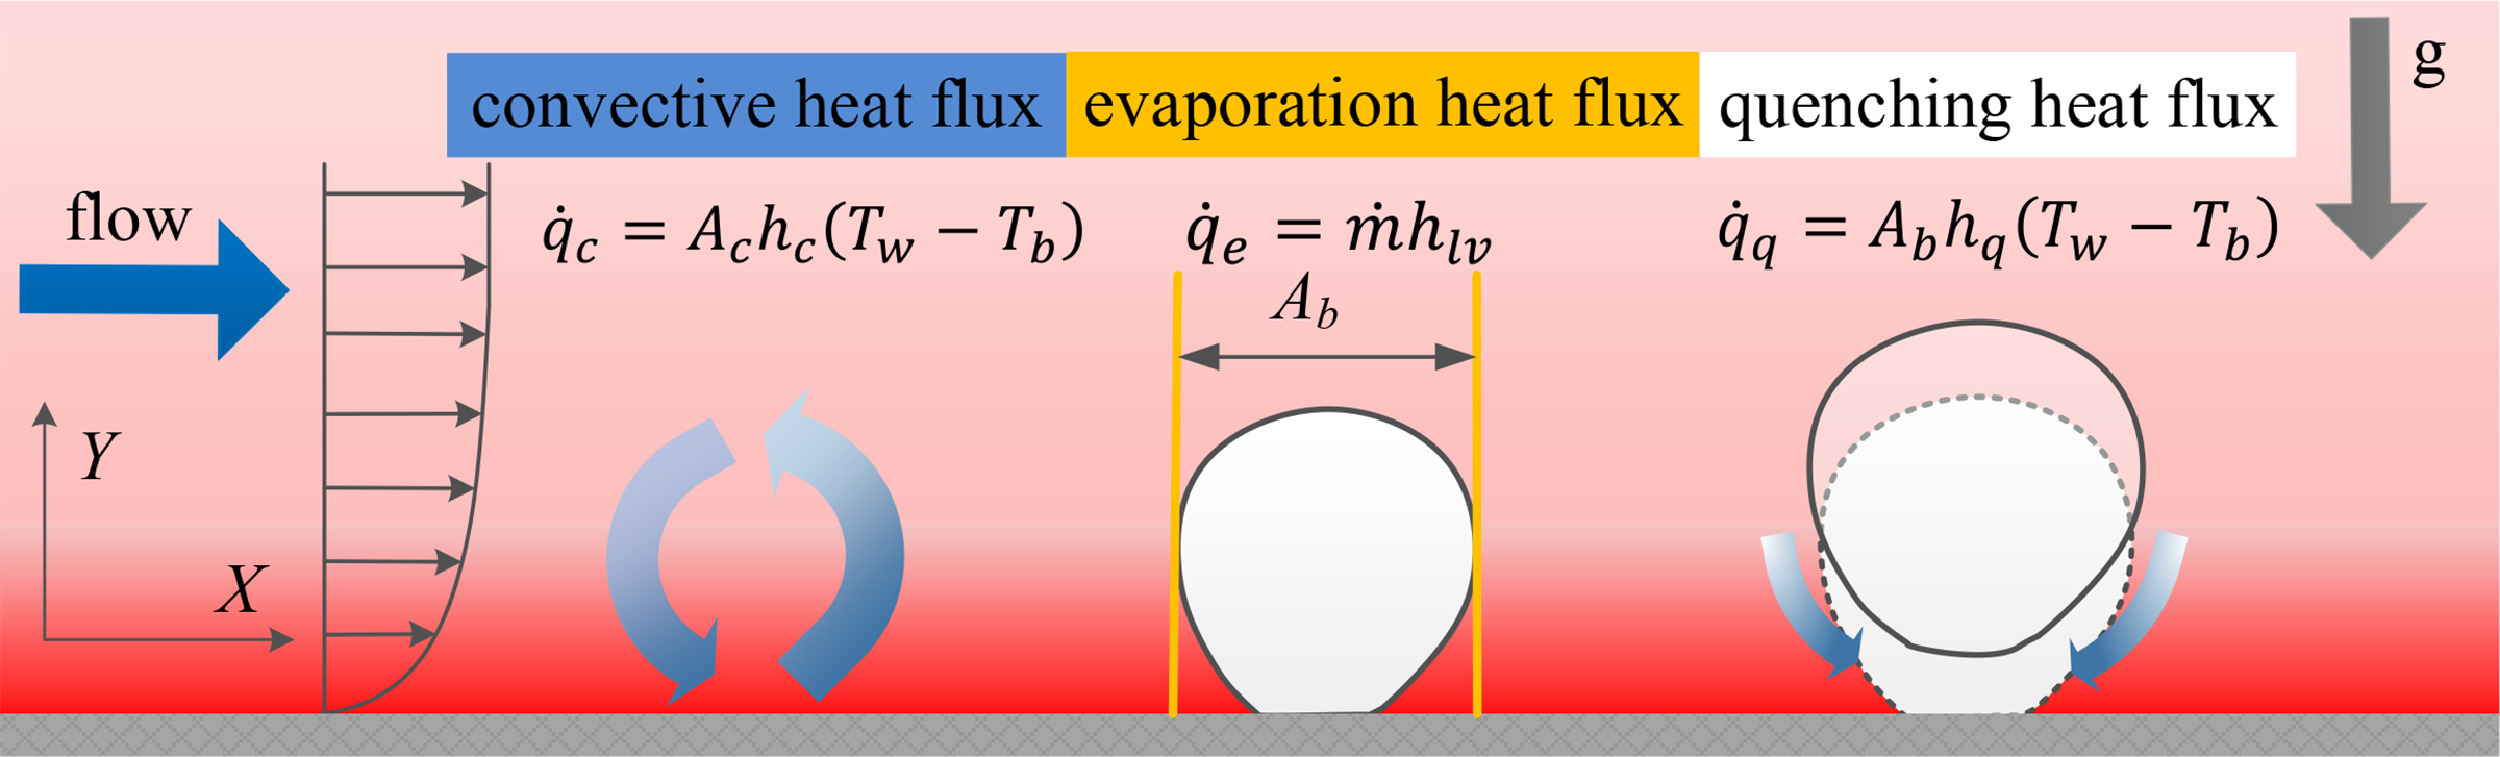
\includegraphics{Figure/Kurul.jpg}
    \caption{Depiction of the wall heat flux partitioning model for subcooled flow boiling from \textcite{ZHOU2021121295}.}
    \label{kurul}
\end{figure}
The model is implemented in :
\begin{lstlisting}[language=c++]
void Flux_parietal_Kurul_Podowski::set_param(Param& param)
\end{lstlisting}
The model implemented is :\\
1) Correction of single phase heat flux
\begin{itemize}
    \item[\small \textcolor{blue}{\ding{109}}]$\texttt{qpk}=\texttt{qpk}_{single\ phase}(1-A_{bub})$,
    \item[\small \textcolor{blue}{\ding{109}}]$\texttt{da\_qpk}=\texttt{da\_qpk}_{single\ phase}(1-A_{bub})$,
    \item[\small \textcolor{blue}{\ding{109}}]$\texttt{dp\_qpk}=\texttt{dp\_qpk}_{single\ phase}(1-A_{bub})$,
    \item[\small \textcolor{blue}{\ding{109}}]$\texttt{dv\_qpk}\texttt{=dv\_qpk}_{single\ phase}(1-A_{bub})$,
    \item[\small \textcolor{blue}{\ding{109}}]$\texttt{dTf\_qpk}=\texttt{dT_f\_qpk}_{single\ phase}(1-A_{bub})$,
    \item[\small \textcolor{blue}{\ding{109}}]$\texttt{dTp\_qpk}=\texttt{dTp\_qpk}_{single\ phase}(1-A_{bub})$.
\end{itemize}
2) Add partitioned heat flux
\begin{itemize}
    \item[\small \textcolor{blue}{\ding{109}}]$\texttt{dTp\_qpk} \pluseq -\texttt{qpk}_{single\ phase}(1-A_{bub})\frac{dA_{bub}}{dT_p}+\frac{dq_{quench}}{dT_p}$,
    \item[\small \textcolor{blue}{\ding{109}}]$\texttt{qpk}  \pluseq  q_{quench}$,
    \item[\small \textcolor{blue}{\ding{109}}]$\texttt{dTf\_qpk} \pluseq \frac{dq_{quench}}{dT_l}$,
    \item[\small \textcolor{blue}{\ding{109}}]$\texttt{qpi}  \pluseq  q_{evap}$,
    \item[\small \textcolor{blue}{\ding{109}}]$\texttt{dTp\_qpi} \pluseq \frac{dq_{evap}}{dT_p}$,
\end{itemize}
with
\begin{itemize}
    \item[\small \textcolor{blue}{\ding{109}}]Evaporation flux $q_{evap}=f_{dep}\frac{\pi d_b^3}{6}\rho_gL_{vap}N_{sites}$
    \item[\small \textcolor{blue}{\ding{109}}]Evaporation flux derivative regarding wall departure $\frac{dq_{evap}}{dT_p} =(\frac{df_{dep}}{dT_p}\frac{\pi d_b^3}{6}N_{sites}+f_{dep}\frac{3\pi d^2}{6}\frac{dd_b}{dT_p}N_{sites}+f_{dep}\frac{\pi d_b^3}{6}\frac{dN_{sites}}{dT_p})\rho_g L_{vap}$.
    \item[\small \textcolor{blue}{\ding{109}}]Quenching flux $q_{quench}=A_{bub}\sqrt{f_{dep}}\frac{2\lambda_l(T_p-T_l)}{\sqrt{\frac{\pi \lambda_l}{\rho_l Cp_l}}}$.
    \item[\small \textcolor{blue}{\ding{109}}]Quenching flux derivative regarding liquid temperature $\frac{d q_{quench}}{d T_l} =A_{bub}\sqrt{f_{dep}}\frac{-2\lambda_l}{\sqrt{\frac{\pi \lambda_l}{\rho_l Cp_l}}}$.
    \item[\small \textcolor{blue}{\ding{109}}]Quenching flux derivative regarding wall temperature $\frac{d q_{quench}}{d T_p} =\frac{d A_{bub}}{dT_p} \sqrt{f_{dep}}\frac{-2\lambda_l}{\sqrt{\frac{\pi \lambda_l}{\rho_l Cp_l}}}+A_{bub}\sqrt{f_{dep}}\frac{2\lambda_l}{\sqrt{\frac{\pi \lambda_l}{\rho_l Cp_l}}}-A_{bub}\frac{1}{2}\frac{df_{dep}}{dT_p}\frac{1}{\sqrt{f_{dep}}}\frac{2\lambda_l(T_p-T_l)}{\sqrt{\frac{\pi \lambda_l}{\rho_l Cp_l}}}$.
    \item[\small \textcolor{blue}{\ding{109}}]Number of evaporation sites $N_{sites}=(210\times{}(T_p-T_{sat}))^{1.8}$.
    \item[\small \textcolor{blue}{\ding{109}}]Number of evaporation sites $N_{sites}=(210\times{}(T_p-T_{sat}))^{1.8}$.
    \item[\small \textcolor{blue}{\ding{109}}]Number of evaporation sites derivative regarding wall temperature $\frac{d N_{sites}}{dT_p} =210\times 1.8(210.(T_p-T_{sat}))^{0.8}$.
    \item[\small \textcolor{blue}{\ding{109}}]Wall bubble diameter $d_b=0.0001(T_p-T_{sat})+0.0014$.
    \item[\small \textcolor{blue}{\ding{109}}]Wall bubble diameter derivative regrading wall temperature $\frac{dd_b}{dT_p}=0.0001$.
    \item[\small \textcolor{blue}{\ding{109}}]Wall bubble total area $A_{bub}=min(1.,\frac{\pi N_{sites}d_b^2}{4})$.
    \item[\small \textcolor{blue}{\ding{109}}]Wall bubble total area derivative regarding wall temperature  $\frac{dA_{bub}}{dT_p} =\frac{\pi d_b^2}{4}\frac{d N_{sites}}{dT_p} + \frac{\pi d_b N_{sites}}{2}\frac{d d_b}{dT_p}$, if $A_{bubbles}\neq 1.$, $0$, otherwise.
    \item[\small \textcolor{blue}{\ding{109}}]Departure frequency $f_dep=\sqrt{\frac{4}{3}\frac{9.81(\rho_l-\rho_g)}{\rho_l}}d_b^{-0.5}$.
    \item[\small \textcolor{blue}{\ding{109}}]Departure frequency derivative regarding wall temperature $\frac{d f_dep}{d T_p}=-0.5\frac{dd_b}{dT_p}d^{-1.5}\sqrt{\frac{4}{3}\frac{9.81(\rho_l-rho_g)}{\rho_l}}$

\end{itemize}

\subsection{Phase change}
The general expression of the phase change mass flux is :
\begin{equation}
    G(\alpha,p,T)
\end{equation}
It needs to be considered when there is a kinetic limit of gas for the phase change, for liquid metals, for example, but it does not apply to water.\\
The model is implemented in :
\begin{lstlisting}[language=c++]
void Changement_phase_base::set_param(Param& param)
\end{lstlisting}
The available input parameters are :
\begin{lstlisting}[language=c++]
    double D_h;           // Hydraulic diameter
    double p;             // Pressure
    const double *alpha;  // Void fraction
    const double *T;      // Temperature
    const double *lambda; // Thermal conductivity
    const double *mu;     // Viscosity
    const double *rho;    // Density
    const double *Cp;     // Calorific capacity
    const double *Lvap;   // Latent heat
    const double *Tsat;   //Phase change saturated temperature
\end{lstlisting}
The phase change mass flux operator must fill dT_G, da_G, dp_G tabs and there derivative so that :
\begin{itemize}
    \item[\small \textcolor{blue}{\ding{109}}]$\texttt{G}$ mass flux
    \item[\small \textcolor{blue}{\ding{109}}] $\texttt{dT\_G}$ mass flux derivative regarding temperature
    \item[\small \textcolor{blue}{\ding{109}}]$\texttt{dp\_G }$ mass flux derivative regarding pressure
    \item[\small \textcolor{blue}{\ding{109}}]$\texttt{da\_G}$ mass flux derivative regarding void fraction
\end{itemize}

\subsubsection{Silver Simpson}
The model is also described in  Silver and Simpson (1949, not found).

The model is implemented as:
\begin{lstlisting}[language=c++]
void Changement_phase_Silver_Simpson::set_param(Param& param)
{
  param.ajouter("lambda_e", &lambda_ec[0]); multiplicative factor for evaporation
  param.ajouter("lambda_c", &lambda_ec[1]); //  multiplicative factor for condensation
  param.ajouter("alpha_min", &alpha_min); // minimal void fraction to activate phase change
  param.ajouter("M", &M, Param::REQUIRED); // molar mass of steam
}
\end{lstlisting}
Default values : $\texttt{lambda\_ec[2]} = { 1, 1 }$, $\texttt{M} = -100.$, $\texttt{alpha\_min} = 0.1$.\\
The model implemented is :
\begin{align}
  &\texttt{dT\_G}_g = \texttt{fac} \times \texttt{var\_a} \times \frac{dT_{Psat}(T_g) - 0.5 \times \frac{Psat(T_g)}{T_g + T_0}}{\sqrt{T_g + T_0}}\\
  &\texttt{dT\_G}_l = \texttt{fac} \times \texttt{var\_a} \times 0.5 \times P \times (T_l + T_0)^{-1.5}\\
  &\texttt{da\_G}_g = \begin{cases} \texttt{fac} \times \texttt{var\_T} \times \texttt{var\_al}, if\  \alpha_g > \text{alpha\_min}, \\ 0,\ otherwise.\end{cases}\\
  &\texttt{da\_G}_l = \begin{cases} \texttt{fac} \times \texttt{var\_T} \times \texttt{var\_ak} \times 1.5 \times \sqrt{\alpha_l}, if\ \alpha_l > \texttt{alpha\_min},\\ 0,\ \text{otherwise}.
  \end{cases}\\
  &\texttt{dp\_G} = - \texttt{fac} \times \frac{\texttt{var\_a}}{\sqrt{T_l + T_0}}\\
  &\texttt{G} = \texttt{fac} \times\texttt{ var\_ak} \times \texttt{var\_al} \times \texttt{var\_T};
\end{align}
with
\begin{itemize}
    \item[\small \textcolor{blue}{\ding{109}}]$T_0 = 273.15$,
    \item[\small \textcolor{blue}{\ding{109}}]$\texttt{var\_ak}=\max(\alpha_g, \texttt{alpha\_min})$,
    \item[\small \textcolor{blue}{\ding{109}}]$\texttt{var\_al}=\parent{\max\parent{\alpha_l,\texttt{alpha\_min}}}^{1.5}$,
    \item[\small \textcolor{blue}{\ding{109}}]$\texttt{var\_a}=\texttt{var\_ak} \times \texttt{var\_al}$,
    \item[\small \textcolor{blue}{\ding{109}}]$\texttt{var\_T} = \frac{Psat(T_g)}{\sqrt{T_g + T_0}}  - \frac{P}{\sqrt{T_l + T_0}}$,
    \item[\small \textcolor{blue}{\ding{109}}]$\texttt{fac} = \lambda_{ec}[var_T < 0] \frac{4}{D_h}\sqrt{\frac{\texttt{M}}{2\texttt{M_{PI}}8.314}}$
\end{itemize}

\section{Analytical terms as source terms}\label{sec:analytical}
This section describes some analytical terms that are implemented as source terms in matrix.
%%
\subsection{Pressure term in energy equation}
This term arises from the averaging of the pressure work term due to the transport of internal energy instead of enthalpy. It represents the pressure work associated with changes in the distribution of void fraction. Its expression is :
\begin{equation}
    -P\parent{\frac{\partial \alpha_k}{\partial t}+\nabla \cdot (\alpha_k v_k)}
\end{equation}
It is implemented in:
\begin{lstlisting}[language=c++]
void Source_Travail_pression_Elem_base::set_param(Param& param)
\end{lstlisting}
\subsection{Gravity}
Gravity is treated as a source term in \texttt{Pb_multiphase} and can't be as other problems from TrioCFD and TRUST. \\
The common way to add gravity is to add in the momentum equation a source. For example, with 2 phases :
\begin{lstlisting}[language=c++]
source_qdm Champ_Fonc_xyz dom 6 0 0 0 0 -9.81 -9.81
\end{lstlisting}
One must use \texttt{Gravite_Multiphase} to get gravity in momentum equation when using drift correlation.
The model is implemented as :
\begin{lstlisting}[language=c++]
void Gravite_Multiphase::set_param(Param& param)
{
  Noms noms(D), unites(D);
  noms[0] = "gravite";
  unites[0] = "m/s^2";
  Motcle typeChamp = "champ_elem" ;
  const Domaine_dis& z = ref_cast(Domaine_dis, pb.domaine_dis());
  dis.discretiser_champ(typeChamp, z.valeur(), scalaire, noms , unites, D, 0, gravite_);
}
\end{lstlisting}

\section{Injected sources of mass}\label{sec:injection}
It is necessary in order to simulate injectors of non-condensable bubbles, otherwise it boils.
\subsection{Injection of mass}
The model is implemented in:
\begin{lstlisting}[language=c++]
void Source_injection_masse_base::set_param(Param& param)
{
  Cerr << "Lecture du Champ de masse injectee" << finl;

  Champ_Don flux_masse_lu_;
  Motcle type;
  is >> type;

  flux_masse_lu_.typer(type);
  Champ_Don_base& ch_flux_masse_lu_ = ref_cast(Champ_Don_base,flux_masse_lu_.valeur());
  is >> ch_flux_masse_lu_;
  const int nb_comp = ch_flux_masse_lu_.nb_comp();

  equation().probleme().discretisation().discretiser_champ("champ_elem", equation().domaine_dis(), "pp", "1",nb_comp,0., flux_masse_);
  flux_masse_lu_->fixer_nb_comp(nb_comp);
  if (ch_flux_masse_lu_.le_nom()=="anonyme") ch_flux_masse_lu_.nommer("Flux_masse_injectee");

  for (int n = 0; n < nb_comp; n++) flux_masse_lu_->fixer_nom_compo(n, ch_flux_masse_lu_.le_nom() + (nb_comp > 1 ? Nom(n) :""));
  for (int n = 0; n < nb_comp; n++) flux_masse_->fixer_nom_compo(n, ch_flux_masse_lu_.le_nom() + (nb_comp > 1 ? Nom(n) :""));
  equation().discretisation().nommer_completer_champ_physique(equation().domaine_dis(),ch_flux_masse_lu_.le_nom(),"1/s",flux_masse_lu_,equation().probleme());
  equation().discretisation().nommer_completer_champ_physique(equation().domaine_dis(),ch_flux_masse_lu_.le_nom(),"1/s",flux_masse_,equation().probleme());
  flux_masse_.valeur().valeurs() = 0;
  flux_masse_.valeur().affecter(flux_masse_lu_);

  const Pb_Multiphase& pb = ref_cast(Pb_Multiphase, equation().probleme());
  int N = pb.nb_phases();
  if (N != flux_masse_.valeurs().line_size()) Process::exit(que_suis_je() + " : you must input as many fluxes as there are phases !!");

  return is;
}
\end{lstlisting}
In the mass equation:
\begin{equation}
    \texttt{secmem}  \pluseq  \rho_k f_{inj}
\end{equation}

\subsection{Momentum correction}
When a fluid flow is injected through a wall with zero momentum via a Neumann boundary condition on the mass equation, it is necessary to correct the momentum equation.

The model is implemented in:
\begin{lstlisting}[language=c++]
void Injection_QDM_nulle_PolyMAC_P0::set_param(Param& param)
{
  Param param(que_suis_je());
  param.ajouter("beta", &beta_);
  param.lire_avec_accolades_depuis(is);
}
\end{lstlisting}
Default values : $\texttt{beta\_} =1$.\\
Case 1: when bubbles are injected at the wall if not face from boundary
\begin{align}
    &\texttt{f\_a\_masse}=\rho_g U_{inj}\\
    &\texttt{f\_a}=\rho_g U_{inj}
\end{align}
corr-ajouter\_inj
\begin{align}
  &\texttt{secmem} \minuseq \texttt{surface}\times \texttt{f\_a\_masse}\times U^n\times \texttt{beta\_}\\
  &M_v \pluseq \texttt{surface}\times \texttt{f\_a\_masse}\times \texttt{beta\_}
\end{align}
Case 2: wall boiling if not face from boundary
\begin{align}
&\texttt{G}=\frac{q_p}{L_{vap}}\\
&\texttt{f\_a\_masse}  \minuseq \frac{\texttt{G}}{\texttt{surface}}\times \begin{cases} \frac{1}{\rho_g},\text{ if in gas,}\\-\frac{1}{\rho_l},\text{ if in liquid.} \end{cases}\\
&\texttt{f\_a}  \minuseq \frac{\texttt{G}}{\texttt{surface}}\times \begin{cases} 1,\text{ if in gas,}\\-1,\text{ if in liquid.}\end{cases}
\end{align}
corr-ajouter\_inj
\begin{align}
  &\texttt{secmem}  \minuseq  \texttt{surface} \times \texttt{f\_a\_masse}\times U^n\times \texttt{beta\_}\\
  &M_v \pluseq \texttt{surface}\times \texttt{f\_a\_masse}\times \texttt{beta\_}
\end{align}

%%%
\section{Equivalent diameter for dispersed phase\label{sec:diam-mgmt}}
\label{sec:IATE}
A fundamental aspect of modeling the interaction between liquid and gas phases lies in precisely predicting the concentration of interfaces. Some models rely on either the interfacial area concentration ($ai$) or an equivalent diameter ($Dsm$). In this context, the dispersed fluid is depicted as a collection of bubbles with diverse diameters, which essentially acts as a topological description for the fluid stage. This dispersed fluid is distinguished by two interlinked attributes: a distribution of bubble diameters and the concentration of interfaces. We can define the Sauter-Mean Diameter ($Dsm$) of the distribution ($f_d$) of sizes D as :
\begin{equation}
Dsm=\frac{\int f_dD^3 dD}{\int f_d D^2 dD}
\end{equation}
The relationship between the void fraction ($\alpha$) and the Sauter-Mean Diameter ($Dsm$)  hinges on calculating the area concentration per unit volume ($A_i=\pi D^2$). This relationship can be expressed as follows :
\begin{equation}
Dsm=\frac{\int f_dD^3 dD}{\int f_d D^2 dD}=6\frac{\int f_d V dv}{\int f_d A_i dV}=6\frac{\alpha}{ai}
\end{equation}
Finally, to have a correct representation of the dispersed phase, it is sufficient to impose an equivalent diameter, but it is also possible to add a transport equation for the interfacial area concentration.

%%
\subsection{User defined diameter}\label{Dsmuserdefine}

%
\subsubsection{Uniform diameter}\mbox{}
It is possible to simply impose a constant diameter at every point in space. The model is implemented in \texttt{Diametre_bulles_constant} :
\begin{lstlisting}[language=c++]
void Diametre_bulles_constant::set_param(Param& param)
{
  Param param(que_suis_je());
  param.ajouter("diametre", &d_bulle_, Param::REQUIRED);
  param.lire_avec_accolades_depuis(is);

  Pb_Multiphase& pb = ref_cast(Pb_Multiphase, pb_.valeur());
  int N = pb.nb_phases();
  const Discret_Thyd& dis=ref_cast(Discret_Thyd,pb.discretisation());
  Noms noms(N), unites(N);
  noms[0] = "diametre_bulles";
  unites[0] = "m";
  Motcle typeChamp = "champ_elem" ;
  const Domaine_dis& z = ref_cast(Domaine_dis, pb.domaine_dis());
  dis.discretiser_champ(typeChamp, z.valeur(), scalaire, noms , unites, N, 0, diametres_);

  champs_compris_.ajoute_champ(diametres_);

  for (int n = 0; n < pb.nb_phases(); n++) //recherche de n_l, n_g : phase {liquide,gaz}_continu en priorite
    if (pb.nom_phase(n).debute_par("liquide") && (n_l < 0 || pb.nom_phase(n).finit_par("continu")))  n_l = n;
  if (n_l < 0) Process::exit(que_suis_je() + " : liquid phase not found!");

  DoubleTab& tab_diametres = diametres_->valeurs();
  for (int i = 0 ; i < tab_diametres.dimension_tot(0) ; i++)
    for (int n = 0 ; n <N ; n++)
      if (n!=n_l) tab_diametres(i, n) = d_bulle_;

  return is;
}
\end{lstlisting}
Default value : $\texttt{d\_ bulle\_} =-100$.

%
\subsubsection{Non-uniform diameter}
It is possible to impose a user-defined diameter that varies spatially through the TRUST fields. The model is implemented in \texttt{Diametre_bulles_champ} :
\begin{lstlisting}[language=c++]
void Diametre_bulles_champ::set_param(Param& param)
{
  Champ_Don diametres_don_;
  is >> diametres_don_;

  Pb_Multiphase& pb = ref_cast(Pb_Multiphase, pb_.valeur());
  int N = pb.nb_phases();
  const Discret_Thyd& dis=ref_cast(Discret_Thyd,pb.discretisation());
  Noms noms(N), unites(N);
  noms[0] = "diametre_bulles";
  unites[0] = "m";
  Motcle typeChamp = "champ_elem" ;
  const Domaine_dis& z = ref_cast(Domaine_dis, pb.domaine_dis());
  dis.discretiser_champ(typeChamp, z.valeur(), scalaire, noms , unites, N, 0, diametres_);
  champs_compris_.ajoute_champ(diametres_);
  diametres_->affecter(diametres_don_.valeur());
  diametres_.valeurs().echange_espace_virtuel();
  return is;
}
\end{lstlisting}
Default value : $\texttt{d\_ bulle\_ }=-100$.

%%
\subsection{Interfacial area concentration with 1 group (incoming)}\label{Dsmu1grp}

%
\subsubsection{The general equation}
Two separated size-group methods are popular for the prediction of interfacial area concentration. One based on having an arbitrary number of groups to reproduce a distribution, referred as MUSIG or i-MUSIG \cite{Wang2005a,Das2010a,Liao2011} and the other reproducing the distribution thanks to the Mean Sauter diameter referred as IATE. The generalized Interfacial Area Transport Equation (IATE) developed by Kocamustafaogullari and Ishii \cite{Kocamustafaogullari,Kocamustafaogullari1994b}
The general expression for adiabatic flows with $\psi^{internal}_{j}$ a source term and $\psi^{intergroup}_j$ an intergroup term is then : \\

\begin{equation}
\frac{\partial a_{i}}{\partial t}+\underbrace{\nabla.(\mathbf{U} a_{i})}_{\colorbox{codebackground}{\color{codekeyword3} convection}}=\underbrace{\frac{2}{3}\frac{a_{i}}{\alpha}\frac{D\alpha}{Dt}}_{\colorbox{codebackground}{\color{codekeyword3} source\ of\ volume\ change}}+\underbrace{\color{myteal}\sum_j \psi^{intergroup}_{j}}_{\colorbox{codebackground}{\color{codekeyword3} intergroup\ sources}}+\underbrace{\color{myteal}\sum_j \psi^{internal}_{j}}_{\colorbox{codebackground}{\color{codekeyword3} intragroup sources}}.
\end{equation}
The terms in green need new modeling linked to coalescence and break-up.
Let's remind that :
\begin{equation}
 \frac{D\alpha\rho_g}{Dt}=\alpha\frac{d\rho_g}{dt}+\rho_g\frac{D\alpha}{Dt}=\Gamma_{transfer}+\Gamma_{nucleation}
 \end{equation}
Then we can substitute :
\begin{equation}
 \frac{D\alpha}{Dt}=\frac{1}{\rho_g}(\Gamma_{transfer}+\Gamma_{nucleation}-\alpha\frac{d\rho_g}{dt})
 \end{equation}
It gives the following equation :
\begin{equation}
\begin{aligned}
\frac{\partial a_{i}}{\partial t}+\underbrace{\nabla.(\mathbf{U} a_{i})}_{\colorbox{codebackground}{\color{codekeyword3} convection}}=\underbrace{-\frac{2}{3}\frac{a_{i}}{\rho_g}\frac{d\rho_g}{dt}}_{\colorbox{codebackground}{\color{codekeyword3} Density\ change}}+\underbrace{\frac{2}{3}\frac{a_{i}}{\alpha}\frac{\Gamma_{transfer}}{\rho_g}}_{\colorbox{codebackground}{\color{codekeyword3} Condensation}}+\underbrace{\frac{2}{3}\frac{a_{i}}{\alpha}\frac{\Gamma_{nucleation}}{\rho_g}}_{\colorbox{codebackground}{\color{codekeyword3} Nucleation}}&+ & \\\underbrace{\color{myteal} \sum_j \psi^{intergroup}_{j}}_{\colorbox{codebackground}{\color{codekeyword3} intergroup\ sources}}+\underbrace{\color{myteal} \sum_j \psi^{internal}_{j}}_{\colorbox{codebackground}{\color{codekeyword3} intragroup sources}}.
\end{aligned}
\end{equation}
The {\colorbox{codebackground}{\color{codekeyword3} Density\ change}} model is :
\begin{equation}
    -\frac{2}{3}\frac{a_{i}}{\rho_g}\frac{d\rho_g}{dt}
\end{equation}
The {\colorbox{codebackground}{\color{codekeyword3} Density\ change}} is implemented in \texttt{Variation_rho_Elem_PolyMAC_P0} :
\begin{lstlisting}[language=c++]
Void Variation_rho::set_param(Param& param)
\end{lstlisting}
It fills the following matrices :
\begin{align}
    &M_{ai} \minuseq  \frac{2}{3}\frac{1-\frac{\rho_g^{n-1}}{\rho_g^n}}{\Delta t}\\
    &M_{T} \minuseq  \frac{2}{3} \frac{a^n_i}{\Delta t} \frac{\rho_g^{n-1}}{(\rho_g^{n})^2}(-\texttt{dT\_rho})\\
    &M_{P} \minuseq  \frac{2}{3}\frac{a^n_i}{\Delta t} \frac{\rho_g^{n-1}}{(\rho_g^{n})^2}(-\texttt{dP\_rho})\\
    &\texttt{secmem} \pluseq  \frac{2}{3}a^n_i\frac{1-\frac{\rho_g^{n-1}}{\rho_g^n}}{\Delta t}
\end{align}
For example, the chain rule for the temperature gives :
\begin{equation}
    \frac{d(\frac{1}{\rho_g}\frac{d\rho_g}{dt})}{dT}=\frac{d\rho_g}{dT}\Bigg(\frac{d}{d\rho_g}(\frac{1}{\rho_g})\frac{d\rho_g}{dt}+\frac{1}{\rho_g}\frac{d}{d\rho_g}(\frac{d\rho_g}{dt}) \Bigg)=\frac{d\rho_g}{dT}\Bigg(-(\frac{1}{\rho_g^2})\frac{d\rho_g}{dt}+\frac{1}{\rho_g}\frac{d}{d\rho_g}(\frac{d\rho_g}{dt}) \Bigg)
\end{equation}
Regarding the discreet form, it gives :
\begin{equation}
   \frac{d\rho_g}{dT}\Bigg(-(\frac{1}{(\rho_g^n)^2})\frac{\rho_g^n-\rho_g^{n-1}}{\Delta t}+\frac{1}{\rho_g^n\Delta t}\Bigg)=\frac{1}{\Delta t}\frac{d\rho_g}{dT}\Bigg(\frac{\rho_g^{n-1}}{(\rho_g^n)^2}\Bigg)
\end{equation}
The {\colorbox{codebackground}{\color{codekeyword3} Condensation}} model is :
\begin{equation}
    \frac{2}{3}\frac{a_i}{\alpha \rho_g} G,
\end{equation}
with G given by a correlation.\\
The {\colorbox{codebackground}{\color{codekeyword3} Condensation}} term is implemented in \texttt{Source_Flux_interfacial_base} as :
\begin{equation}
    \texttt{secmem}  \pluseq  \frac{2}{3}\frac{a_i^n}{\alpha^n\rho_g^n} G^n
\end{equation}
If the condensation is not making the phase evanescent then :
\begin{align}
    &M_\alpha  \minuseq  \frac{-2}{3}\frac{a_i^n}{(\alpha^n)^2}\rho_g^n G^n\\
    &M_T  \minuseq  \frac{-2}{3}\frac{a_i^n}{\alpha^n(\rho_g^n)^2} G^n \frac{d\rho_l}{dT}+\frac{2}{3}\frac{a_i^n}{\alpha^n\rho_g} \frac{dG}{dT}\\
    &M_P  \minuseq  \frac{-2}{3}\frac{a_i^n}{\alpha^n(\rho_g^n)^2} G^n \frac{d\rho_g}{dP}+\frac{2}{3}\frac{a_i^n}{\alpha^n\rho_g} \frac{dG}{dP}\\
    &M_{a_i}  \minuseq  \frac{2}{3}\frac{1}{\alpha^n\rho_g^n} G^n
\end{align}

For the other source terms, refer to the models.

%
\subsubsection{The Yao Morel model}
The model is described in \textcite{YAO2004307}.

The equation is:
\begin{equation}
\frac{\partial a_{i}}{\partial t}+\underbrace{\nabla.(\mathbf{U} a_{i})}_{\colorbox{codebackground}{\color{codekeyword3} convection}}=\underbrace{\frac{2}{3}\frac{a_{i}}{\alpha}(\frac{\Gamma_{condensation}}{\rho_g}-\frac{\alpha_g}{\rho_g} \frac{d \rho_g}{d t})}_{\colorbox{codebackground}{\color{codekeyword3} source\ of\ volume\ change}}+\underbrace{\pi d_{dep}^2\Phi_N}_{\colorbox{codebackground}{\color{codekeyword3} Nucleation}}+\underbrace{\frac{36\pi}{3}(\frac{\alpha}{a_i})^2{\color{myteal}\Phi_{coal}}}_{\colorbox{codebackground}{\color{codekeyword3} Coalescence}}+\underbrace{\frac{36\pi}{3}(\frac{\alpha}{a_i})^2{\color{myteal}\Phi_{breakup}}}_{\colorbox{codebackground}{\color{codekeyword3}  Break-up}}.
\end{equation}
The {\colorbox{codebackground}{\color{codekeyword3} Coalescence}} model is :
\begin{equation}
\begin{aligned}
		\frac{36\pi}{3}(\frac{\alpha}{a_i})^2\Phi_{Coal} =- \frac{36\pi}{3}(\frac{\alpha}{a_i})^2 (\varepsilon d_b)^{1/3} \cdot \frac{\alpha^2}{d_b^4} \cdot K_{c1} \cdot \frac{1}{g(\alpha) + K_{c2}\alpha \sqrt{We/We_{cr}}} \cdot \text{exp}\left(-K_{c3} \sqrt{\frac{We}{We_{cr}}}\right)& & \\ = {\color{mydarkorchid} \frac{\pi}{3\times 6^{5/3}}\alpha^{1/3}a_i^{5/3}\varepsilon^{1/3}} \cdot {\color{myslateblue} K_{c1} \frac{-1}{g(\alpha) + K_{c2}\alpha \sqrt{We/We_{cr}}} \cdot \text{exp}\left(-K_{c3} \sqrt{\frac{We}{We_{cr}}}\right)},
\end{aligned}
\end{equation}
with $K_{c1} = 2.86$, $K_{c2} = 1.922$, $K_{c3} = 1.017$, $We_{cr} = 1.24$, $g(\alpha) = \frac{\alpha_\text{max}^{1/3}-\alpha^{1/3}}{\alpha_\text{max}^{1/3}}$, $\alpha_\text{max} = \frac{\pi}{6}$.\\
The {\colorbox{codebackground}{\color{codekeyword3} Coalescence}} model is implemented as $\frac{36\pi}{3}(\frac{\alpha}{a_i})^2\Phi_{Coal}={\color{mydarkorchid}f_1(\alpha,ai,k,\varepsilon)}{\color{myslateblue} f_2(\alpha,ai,k,\varepsilon)}$ so that for the sake of simplicity $d({\color{mydarkorchid}f_1}{\color{myslateblue} f_2})={\color{myslateblue} f_2}d{\color{mydarkorchid} f_1}$  in {\color{mydarkorchid} Coalescence_bulles_1groupe_PolyMAC_P0} :
\begin{lstlisting}[language=c++]
void Coalescence_bulles_1groupe_PolyMAC_P0::set_param(Param& param)
{
  Param param(que_suis_je());
  param.ajouter("beta_k", &beta_k_);
}
\end{lstlisting}
and {\color{myslateblue} Coalescence_bulles_1groupe_Yao_Morel}:
\begin{lstlisting}[language=c++]
void Coalescence_bulles_1groupe_Yao_Morel::set_param(Param& param)
\end{lstlisting}
Default values : $\texttt{beta\_k\_} = 0.09$, $\texttt{Kc1} = 2.86$, $\texttt{Kc2} = 1.922$, $\texttt{Kc3} = 1.017$,
$\texttt{alpha\_max\_1\_3} = (\frac{\pi}{6})^{1/3}$, $\texttt{We\_cr} = 1.24$.\\
{\color{red} Warning} : The following part describes the matrix filling for the $k-\varepsilon$ model, as an example, but it is currently not implemented since only the $k-\tau$ and $k-\omega$ models are available and are the only ones implemented for the source terms.\\
For the $k-\varepsilon$ model :
\begin{align}
    &M_{\alpha} \minuseq \frac{\pi}{3\times 6^{5/3}}\frac{1}{3}(\alpha^n)^{-2/3}(a_i^n)^{5/3}(\varepsilon^n)^{1/3} {\color{myslateblue} f_2^n}\\
    &M_{a_i} \minuseq \frac{\pi}{3\times 6^{5/3}}\frac{5}{3}(\alpha^n)^{1/3}(a_i^n)^{2/3}(\varepsilon^n)^{1/3} {\color{myslateblue} f_2^n}\\
    &M_{k}=0\\
    &M_{\varepsilon} \minuseq \frac{\pi}{3\times 6^{5/3}}\frac{1}{3}(\alpha^n)^{-2/3}(a_i^n)^{5/3}(\varepsilon^n)^{-2/3} {\color{myslateblue} f_2^n}\\
    &\text{secmem} \pluseq \frac{\pi}{3\times 6^{5/3}}(\alpha^n)^{1/3}(a_i^n)^{5/3}(\varepsilon^n)^{1/3} {\color{myslateblue} f_2^n}
\end{align}
If the $k-\tau$ turbulence model is used,
\begin{equation}
\varepsilon = \frac{k^2}{\text{max}(k\tau, \texttt{visc\_turb.limiteur()} \nu_l)}\times \texttt{beta\_k\_}.
\end{equation}
If the $k-\omega$ turbulence model is used,
\begin{equation}
\varepsilon = k \times \omega \times\texttt{ beta\_k\_}.
\end{equation}
The {\colorbox{codebackground}{\color{codekeyword3}  Break-up}} model is :
\begin{equation}
\begin{aligned}
		\frac{36\pi}{3}\parent{\frac{\alpha}{a_i}}^2\Phi_{\text{breakup}} =- \frac{36\pi}{3}\parent{\frac{\alpha}{a_i}}^2 \parent{\varepsilon d_b}^{1/3} \cdot \frac{\alpha(1-\alpha)}{d_b^4} \cdot K_{b1} \cdot \frac{1}{1 + K_{b2}\alpha_l \sqrt{We/We_{cr}}} \cdot \text{exp}\left(- \frac{We}{We_{cr}}\right)& & \\ = {\color{mydarkorchid} \frac{\pi}{3\times 6^{5/3}}\alpha^{-2/3}(1-\alpha)a_i^{5/3}\varepsilon^{1/3}} \cdot {\color{myslateblue} K_{b1} \cdot \frac{1}{1 + K_{b2}(1-\alpha) \sqrt{We/We_{cr}}} \cdot \text{exp}\left(- \frac{We}{We_{cr}}\right)},
\end{aligned}
\end{equation}
with $K_{b1} = 1.6$, $K_{b2} = 0.42$, $We_{cr} = 1.24$.

The {\colorbox{codebackground}{\color{codekeyword3}  Break-up}} model is implemented as $\frac{36\pi}{3}\parent{\frac{\alpha}{a_i}}^2\Phi_{\text{breakup}}={\color{mydarkorchid}f_1(\alpha,ai,k,\varepsilon)}{\color{myslateblue} f_2(\alpha,ai,k,\varepsilon)}$ so that for the sake of simplicity $d({\color{mydarkorchid}f_1}{\color{myslateblue} f_2})={\color{myslateblue} f_2}d{\color{mydarkorchid} f_1}$  in {\color{mydarkorchid} Rupture_bulles_1groupe_PolyMAC_P0} :
\begin{lstlisting}[language=c++]
void Rupture_bulles_1groupe_PolyMAC_P0::set_param(Param& param)
{
  Param param(que_suis_je());
  param.ajouter("beta_k", &beta_k_);
}
\end{lstlisting}
and {\color{myslateblue} Rupture_bulles_1groupe_Yao_Morel}:
\begin{lstlisting}[language=c++]
void Rupture_bulles_1groupe_Yao_Morel::set_param(Param& param)
\end{lstlisting}
Default values: $\texttt{beta\_k\_} = 0.09$, $\texttt{Kb1} = 1.6$, $\texttt{Kb2} = 0.42$, $\texttt{We\_cr} = 1.24$.\\
{\color{red} Warning} : The following part describes the matrix filling for the $k-\varepsilon$ model, as an example, but it is currently not implemented since only the $k-\tau$ and $k-\omega$ models are available and are the only ones implemented for the source terms.\\
For the $k-\varepsilon$ model :
\begin{align}
    &M_{\alpha} \minuseq \frac{\pi}{3\times 6^{5/3}}\frac{-2}{3}(\alpha^n)^{-5/3}\alpha_l^n(a_i^n)^{5/3}(\varepsilon^n)^{1/3} {\color{myslateblue} f_2^n}\\
    &M_{\alpha_l} \minuseq \frac{\pi}{3\times 6^{5/3}}(\alpha^n)^{-2/3}(a_i^n)^{5/3}(\varepsilon^n)^{1/3} {\color{myslateblue} f_2^n}\\
    &M_{a_i} \minuseq \frac{\pi}{3\times 6^{5/3}}\frac{5}{3}(\alpha^n)^{1/3}\alpha_l^n(a_i^n)^{2/3}(\varepsilon^n)^{1/3} {\color{myslateblue} f_2^n}\\
    &M_{k}=0\\
    &M_{\varepsilon} \minuseq \frac{\pi}{3\times 6^{5/3}}\frac{1}{3}(\alpha^n)^{-2/3}\alpha_l^n(a_i^n)^{5/3}(\varepsilon^n)^{-2/3} {\color{myslateblue} f_2^n}\\
    &\text{secmem}  \pluseq  \frac{\pi}{3\times 6^{5/3}}\frac{1}{3}(\alpha^n)^{-2/3}\alpha_l^n(a_i^n)^{5/3}(\varepsilon^n)^{-2/3} {\color{myslateblue} f_2^n}\\
\end{align}
If the $k-\tau$ turbulence model is used,
\begin{equation}
\varepsilon=\frac{k^2}{\text{max}(k\tau,\ \texttt{visc_turb.limiteur()} \nu_l)}\times beta\_ k \_.
\end{equation}
If the $k-\omega$ turbulence model is used
\begin{equation}
\varepsilon=k\times \omega\times beta\_ k \_.
\end{equation}
The {\colorbox{codebackground}{\color{codekeyword3}  Nucleation}} model is :
\begin{equation}
		\pi d_{dep}^2\Phi_N = \pi d_{dep}^2\frac{\Phi_{e}}{L_{\text{vap}} \rho_g \frac{\pi}{6}d_\text{dep}^3}=6\frac{\Phi_{\text{nucleation}}}{\text{max}(d_{\text{nuc}},10^{-8})\rho_g L_{\text{vap}}}
\end{equation}
with $\Phi_{e}$ wall heat transfer.

The {\colorbox{codebackground}{\color{codekeyword3}  Nucleation}} model is implemented in Nucleation_paroi_PolyMAC_P0:
\begin{lstlisting}[language=c++]
void Nucleation_paroi_PolyMAC_P0::set_param(Param& param)
\end{lstlisting}
This terms injected only on boundary elements and is fully explicit:
\begin{equation}
    \texttt{secmem} \pluseq 6\frac{\Phi_{\text{nucleation}}^n}{\text{max}(d_{\text{nuc}}^n,10^{-8})\rho_g^n L_{\text{vap}}^n}
\end{equation}

%%
\subsection{Interfacial area concentration with 2 groups (incoming)}

%
\subsubsection{The equations}
A particular case of the solution can be obtained if we consider two groups of bubbles. For example, experimentally a limit can be observed between quasi-spherical and distorted bubbles. Then we can separate the distribution of those groups into 2 distinct distributions on either side of the critical diameter $Dsmc=4\sqrt{\tfrac{\sigma}{g(\rho_l-\rho_g)}}$, with $\sigma$ the surface tension, $g$ gravity and $\rho_g$ and $\rho_l$ respectively the densities of the gas and the liquid. For the first group we get :
\begin{equation}
\begin{aligned}
\frac{\partial a_{i1}}{\partial t}+\underbrace{\nabla\parent{a_{i1}\mathbf{U}_{g1}}}_{\colorbox{codebackground}{\color{codekeyword3} convection}}=&\underbrace{\frac{2}{3}\frac{a_{i1}}{\alpha_{g1}}\parent{-\frac{\alpha_{g1}}{\rho_g}\frac{d \rho_g}{dt}}}_{\colorbox{codebackground}{\color{codekeyword3} Density\ change}}-\underbrace{\chi_d\parent{\frac{D_{smc}}{D_{sm1}}}^2\frac{a_{i1}}{\alpha_{g1}}\parent{-\frac{\alpha_{g1}}{\rho_g}\frac{d \rho_g}{dt}}}_{\colorbox{codebackground}{\color{codekeyword3} Density\ sliding}}  \\
&+\underbrace{\frac{2}{3}\frac{a_{i1}}{\alpha_{g1}}\parent{\frac{\color{myteal}\Gamma_{g1}}{\rho_g}}}_{\colorbox{codebackground}{\color{codekeyword3} Mass\ transfer}}-\underbrace{\chi_d\parent{\frac{D_{smc}}{D_{sm1}}}^2\frac{a_{i1}}{\alpha_{g1}}\parent{\frac{\color{myteal}\Gamma_{g1}}{\rho_g}}}_{\colorbox{codebackground}{\color{codekeyword3} Mass\ transfer\ sliding}} \\
&+\underbrace{\color{myteal}\sum_j \psi^{\text{intergroup}}_{1j}}_{\colorbox{codebackground}{\color{codekeyword3} intergroup\ sources}}+\underbrace{\color{myteal}\sum_j \psi^{\text{internal}}_{1j}}_{\colorbox{codebackground}{\color{codekeyword3} intragroup sources}}.
\end{aligned}
\end{equation}
For the second group, we get:
\begin{equation}
\begin{aligned}
\frac{\partial a_{i2}}{\partial t}+\underbrace{\nabla\parent{a_{i2}\mathbf{U}_{g2}}}_{\colorbox{codebackground}{\color{codekeyword3} convection}}=\underbrace{\frac{2}{3}\frac{a_{i2}}{\alpha_{g2}}\parent{-\frac{\alpha_{g2}}{\rho_g}\frac{d \rho_g}{dt}}}_{\colorbox{codebackground}{\color{codekeyword3} Density\ change}}+\underbrace{\chi_d\parent{\frac{D_{smc}}{D_{sm1}}}^2\frac{a_{i1}}{\alpha_{g1}}\parent{-\frac{\alpha_{g1}}{\rho_g}\frac{d \rho_g}{dt}}}_{\colorbox{codebackground}{\color{codekeyword3} Density\ sliding}}&+ & \\
\underbrace{\frac{2}{3}\frac{a_{i2}}{\alpha_{g2}}\parent{\frac{\color{myteal}\Gamma_{g2}}{\rho_g}}}_{\colorbox{codebackground}{\color{codekeyword3} Mass\ transfer}} +\underbrace{\chi_d\parent{\frac{D_{smc}}{D_{sm1}}}^2\frac{a_{i1}}{\alpha_{g1}}\parent{\frac{\color{myteal}\Gamma_{g1}}{\rho_g} }}_{\colorbox{codebackground}{\color{codekeyword3} Mass\ transfer\ sliding}} +& \\
\underbrace{\color{myteal}\sum_j \psi^{\text{intergroup}}_{2j}}_{\colorbox{codebackground}{\color{codekeyword3} intergroup\ sources}}+\underbrace{\color{myteal}\sum_j \psi^{\text{internal}}_{2j}}_{\colorbox{codebackground}{\color{codekeyword3} intragroup sources}}.
\end{aligned}
\end{equation}
The different mass transfer are:
\begin{equation}
\begin{aligned}
\Gamma_{g1}=\underbrace{-\frac{\rho_g}{1+\chi_d \parent{\frac{Dsmc}{Dsm1}}^3}{\color{myteal}\sum_j \eta^{inter}_j}}_{\colorbox{codebackground}{\color{codekeyword3} Intergroup}}+ \underbrace{\frac{\chi_d\parent{\frac{D_{smc}}{D_{sm1}}}^3}{1+\chi_d \parent{\frac{Dsmc}{Dsm1}}^3}\alpha_{g1}\parent{\frac{d\rho_{g}}{dt}}}_{\colorbox{codebackground}{\color{codekeyword3} Density\ group\ shift}}&+& \\
\underbrace{\frac{1}{1+\chi_d \parent{\frac{Dsmc}{Dsm1}}^3}\Gamma_{\text{condensation g1}}}_{\colorbox{codebackground}{\color{codekeyword3} Condensation}}+\underbrace{\frac{\chi_d\parent{\frac{D_{smc}}{D_{sm1}}}^3}{1+\chi_d \parent{\frac{Dsmc}{Dsm1}}^3}\Gamma_{\text{Nucleation g1}}}_{\colorbox{codebackground}{\color{codekeyword3} Nucleation}}.
\end{aligned}
\end{equation}
\begin{equation}
\begin{aligned}
\Gamma_{g2}=\underbrace{\frac{\rho_g}{1+\chi_d \parent{\frac{Dsmc}{Dsm1}}^3}{\color{myteal}\sum_j \eta^{inter}_j}}_{\colorbox{codebackground}{\color{codekeyword3} Intergroup}}- \underbrace{\frac{\chi_d\parent{\frac{D_{smc}}{D_{sm1}}}^3}{1+\chi_d \parent{\frac{Dsmc}{Dsm1}}^3}\alpha_{g1}\parent{\frac{d\rho_{g}}{dt}}}_{\colorbox{codebackground}{\color{codekeyword3} Density\ group\ shift}}&+& \\
\underbrace{\Gamma_{\text{condensation\ g2}}+\frac{\chi_d \parent{\frac{Dsmc}{Dsm1}}^3}{1+\chi_d \parent{\frac{Dsmc}{Dsm1}}^3}\Gamma_{\text{condensation g1}}}_{\colorbox{codebackground}{\color{codekeyword3} Condensation}}-\underbrace{\frac{\chi_d\parent{\frac{D_{smc}}{D_{sm1}}}^3}{1+\chi_d \parent{\frac{Dsmc}{Dsm1}}^3}\Gamma_{\text{Nucleation g1}}}_{\colorbox{codebackground}{\color{codekeyword3} Nucleation}}.
\end{aligned}
\end{equation}
$\chi_d$ is equal to $1$ for a uniform distribution profile. Indeed, because there is no prior determination of the form of the solution of the distribution, the easiest from to consider is a uniform distribution.
During the averaging process proposed in \cite{Kataoka2012} , two new terms emerged from the instantaneous equation: a diffusion term and a lift term. For example, the diffusion term can be implemented as:
\begin{equation}
K\sqrt{u^{\prime 2}}D_{sm}\nabla a_i=K\sqrt{\frac{2k}{3}} D_{sm}\nabla a_i,
\end{equation}
with $K$ a constant equal to $1/3$. However, it is essential to note that these terms have not yet been fully validated in various configurations \cite{Rassame2023}. For the implementation in the code, we must rewrite it to get rid of $D_{sm}$. For the first group we have:
\begin{equation}
\begin{aligned}
\frac{\partial a_{i1}}{\partial t}+\underbrace{\nabla\parent{a_{i1}\mathbf{U}_{g1}}}_{\colorbox{codebackground}{\color{codekeyword3} convection}}=\underbrace{\frac{2}{3}\frac{a_{i1}}{\alpha_{g1}}\parent{-\frac{\alpha_{g1}}{\rho_g}\frac{d \rho_g}{dt}}}_{\colorbox{codebackground}{\color{codekeyword3} Density\ change}}-\underbrace{\frac{\chi_d}{36}D_{smc}^2\parent{\frac{a_{i1}}{\alpha_{g1}}}^3\parent{-\frac{\alpha_{g1}}{\rho_g}\frac{d \rho_g}{dt}}}_{\colorbox{codebackground}{\color{codekeyword3} Density\ sliding}} &+& \\\underbrace{\frac{2}{3}\frac{a_{i1}}{\alpha_{g1}}\parent{\frac{\color{myteal}\Gamma_{g1}}{\rho_g}}}_{\colorbox{codebackground}{\color{codekeyword3} Mass\ transfer}}-\underbrace{\frac{\chi_d}{36}D_{smc}^2\parent{\frac{a_{i1}}{\alpha_{g1}}}^3\parent{\frac{\color{myteal}\Gamma_{g1}}{\rho_g}}}_{\colorbox{codebackground}{\color{codekeyword3} Mass\ transfer\ sliding}}+& \\\underbrace{\color{myteal}\sum_j \psi^{intergroup}_{1j}}_{\colorbox{codebackground}{\color{codekeyword3} intergroup\ sources}}+\underbrace{\color{myteal}\sum_j \psi^{internal}_{1j}}_{\colorbox{codebackground}{\color{codekeyword3} intragroup sources}}.
\end{aligned}
\end{equation}
For the second group, we obtain:
\begin{equation}
\begin{aligned}
\frac{\partial a_{i2}}{\partial t}+\underbrace{\nabla\parent{a_{i2}\mathbf{U}_{g2}}}_{\colorbox{codebackground}{\color{codekeyword3} convection}}=\underbrace{\frac{2}{3}\frac{a_{i2}}{\alpha_{g2}}\parent{-\frac{\alpha_{g2}}{\rho_g}\frac{d \rho_g}{dt}}}_{\colorbox{codebackground}{\color{codekeyword3} Density\ change}}+\underbrace{\frac{\chi_d}{36}D_{smc}^2\parent{\frac{a_{i1}}{\alpha_{g1}}}^3\parent{-\frac{\alpha_{g1}}{\rho_g}\frac{d \rho_g}{dt}}}_{\colorbox{codebackground}{\color{codekeyword3} Density\ sliding}}&+ & \\
\underbrace{\frac{2}{3}\frac{a_{i2}}{\alpha_{g2}}\parent{\frac{\color{myteal}\Gamma_{g2}}{\rho_g}}}_{\colorbox{codebackground}{\color{codekeyword3} Mass\ transfer}} +\underbrace{\frac{\chi_d}{36}D_{smc}^2\parent{\frac{a_{i1}}{\alpha_{g1}}}^3\parent{\frac{\color{myteal}\Gamma_{g1}}{\rho_g} }}_{\colorbox{codebackground}{\color{codekeyword3} Mass\ transfer\ sliding}} +& \\
\underbrace{\color{myteal}\sum_j \psi^{\text{intergroup}}_{2j}}_{\colorbox{codebackground}{\color{codekeyword3} intergroup\ sources}} + \underbrace{\color{myteal}\sum_j \psi^{\text{internal}}_{2j}}_{\colorbox{codebackground}{\color{codekeyword3} intragroup sources}}.
\end{aligned}
\end{equation}
The different mass transfer are:
\begin{equation}
\begin{aligned}
\Gamma_{g1} = \underbrace{-\frac{\rho_g}{1+\frac{\chi_d}{216}Dsmc^3\parent{\frac{a_{i1}}{\alpha_{g1}}}^3}{\color{myteal}\sum_j \eta^{inter}_j}}_{\colorbox{codebackground}{\color{codekeyword3} Intergroup}}+ \underbrace{\frac{\frac{\chi_d}{216}Dsmc^3\parent{\frac{a_{i1}}{\alpha_{g1}}}^3}{1+\frac{\chi_d}{216}Dsmc^3\parent{\frac{a_{i1}}{\alpha_{g1}}}^3}\alpha_{g1}\parent{\frac{d\rho_{g}}{dt}}}_{\colorbox{codebackground}{\color{codekeyword3} Density\ group\ shift}}&+& \\
\underbrace{\frac{1}{1+\frac{\chi_d}{216}Dsmc^3\parent{\frac{a_{i1}}{\alpha_{g1}}}^3}\Gamma_{\text{condensation g1}}}_{\colorbox{codebackground}{\color{codekeyword3} Condensation}}+\underbrace{\frac{\frac{\chi_d}{216}Dsmc^3\parent{\frac{a_{i1}}{\alpha_{g1}}}^3}{1+\frac{\chi_d}{216}Dsmc^3\parent{\frac{a_{i1}}{\alpha_{g1}}}^3}\Gamma_{\text{Nucleation g1}}}_{\colorbox{codebackground}{\color{codekeyword3} Nucleation}}.
\end{aligned}
\end{equation}
\begin{equation}
\begin{aligned}
\Gamma_{g2}=\underbrace{\frac{\rho_g}{1+\frac{\chi_d}{216}Dsmc^3(\frac{a_{i1}}{\alpha_{g1}})^3}{\color{myteal}\sum_j \eta^{inter}_j}}_{\colorbox{codebackground}{\color{codekeyword3} Intergroup}}- \underbrace{\frac{\frac{\chi_d}{216}Dsmc^3(\frac{a_{i1}}{\alpha_{g1}})^3}{1+\frac{\chi_d}{216}Dsmc^3(\frac{a_{i1}}{\alpha_{g1}})^3}\alpha_{g1}\parent{\frac{d\rho_{g}}{dt}}}_{\colorbox{codebackground}{\color{codekeyword3} Density\ group\ shift}}&+& \\
\underbrace{\Gamma_{\text{condensation g2}} + \frac{\frac{\chi_d}{216}Dsmc^3(\frac{a_{i1}}{\alpha_{g1}})^3}{1+\frac{\chi_d}{216}Dsmc^3(\frac{a_{i1}}{\alpha_{g1}})^3}\Gamma_{\text{condensation g1}}}_{\colorbox{codebackground}{\color{codekeyword3} Condensation}}-\underbrace{\frac{\frac{\chi_d}{216}Dsmc^3(\frac{a_{i1}}{\alpha_{g1}})^3}{1+\frac{\chi_d}{216}Dsmc^3(\frac{a_{i1}}{\alpha_{g1}})^3}\Gamma_{\text{Nucleation g1}}}_{\colorbox{codebackground}{\color{codekeyword3} Nucleation}}.
\end{aligned}
\end{equation}

%
\subsubsection{The source terms}
All source term models are based on five categories of mechanism: the Random Collisions (RC), the Wake Entrainment (WE), the Turbulent Impacts (TI), the Shearing-off (SO) and the Surface Instability (SI) (see Figure \ref{bulles}). The RC is a bubble coalescence phenomenon where $2$ bubbles collide and merge because of a turbulent eddy of comparable size. The WE happens when one smaller bubble is in the wake of a bigger one, accelerates and collides it. The TI is due to turbulent eddies that break-up bubbles. The SO is a break-up phenomenon that source from the shearing-off of cap bubbles. The SI is due to the break-up of large bubbles due to their surface instability.\\
The number of processes and the dimensionless coefficient can strongly differ from one model to another :
\begin{itemize}
\item[\small \textcolor{blue}{\ding{109}}] The \textcite{SUN2} model was developed for a $2$ group configuration with a $200 \times  10$ $mm^2$ confined rectangular channel data. The effect of the wall is then very significant. It was performed for liquid superficial velocity between $0.32$ and $2.84$ m/s and gas velocity between $0.39$ and $2.01$ m/s. It deals with cap-bubbly and churn-turbulent flows.\\
\item[\small \textcolor{blue}{\ding{109}}] The \textcite{Smith1} model was developed for a $2$ group configuration with $0.102$ mm and $0.152$ mm diameter pipes. It deals with bubbly, cap-bubbly and churn-turbulent flows. \\
\item[\small \textcolor{blue}{\ding{109}}] The \textcite{Schlegel1} model was developed for a $2$ group configuration with large diameter channels. It deals with bubbly and cap-bubbly flows. Several constitutive relations and correlations were used to tune this model.\\
\item[\small \textcolor{blue}{\ding{109}}] The \textcite{Fu2002} model was developed for a $2$ group configuration for small round pipe.\\
\item[\small \textcolor{blue}{\ding{109}}] \textcite{Dave2016a} proposed new Smith coefficient based on optimization with genetic algorithm on all TOPFLOW DN200 (pipe $195.3$ mm).
\end{itemize}
\begin{figure}[!ht]
    \centering
    \includegraphics[scale=1]{Figure/bulles2.png}
    \caption{Representation of 2 group bubble mechanisms.}
    \label{bulles}
\end{figure}
The coefficients of the previous models are summarized in Table \ref{coeff2grp}.
\begin{table}[!ht]
\begin{center}
\begin{tabular}{c c c c c c }
\toprule
Coefficient & Sun \cite{SUN2} & Smith \cite{Smith1} & Schlegel \cite{Schlegel1} & Fu \cite{Fu2002} & Dave \cite{Dave2016a}\\
\midrule
\rowcolor[gray]{0.9} $C^{(1)}_{RC}$ & $0.005$ &$0.01$ & $0.01$ & $0.0041$ & $0.26$ \\
 $C^{(12,2)}_{RC}$ & $0.005$ & $0.01$ & $0.05$ & $0.005$ & $0.41$ \\
 \rowcolor[gray]{0.9} $C^{(2)}_{RC}$ & $0.005$ & $0.01$ & $0.01$ & $0.005$ & $1.00$ \\
 $C_{RC0}$ & $3.0$ & $3.0$ & $3.0$ & $3.0$ & $3.0$ \\
 \rowcolor[gray]{0.9} $C_{RC1}$ & $3.0$ & $3.0$ & $3.0$  & $3.0$ & $3.0$ \\
 $\alpha_{g1,max}$ & $0.62$ & $0.62$ & $0.62$& $0.75$ & $0.62$ \\
\rowcolor[gray]{0.9} $C^{(1)}_{WE}$ & $0.002$ & $0.002$ & $0.002$ & $0.002$ & $0.001$  \\
$C^{(12,2)}_{WE}$ & $0.002$ & $0.01$ & $0.02$ & $0.015$ & $0.017$\\
\rowcolor[gray]{0.9} $C^{(2)}_{WE}$ & $0.005$ & $0.01$ & $0.05$ & $10.$ & $0.021$  \\
$C^{(1)}_{TI}$ & $0.1$ & $0.05$ & $0.05$ & $0.0085$ & $0.013$  \\
\rowcolor[gray]{0.9} $C^{(12,2)}_{TI}$ & $0.02$ & $0.04$ & $0.02$ & $0.02$ & $0.006$  \\
$C^{(2)}_{TI}$ & $0.02$ & $0.01$ & $0.01$ & $0.02$ & $0.023$ \\
\rowcolor[gray]{0.9} $We_{cr1}$ & $6.5$ & $1.2$ & $1.2$ & $6.0$ & $6.0$  \\
$We_{cr2}$ & $7.0$ & $1.2$ & $ 1.2$ & $6.0$ & $6.0$  \\
\rowcolor[gray]{0.9} $C_{SO}$ & $3.8 \times 10^{-5}$ & $2.5 \times 10^{-5}$ & $5.0 \times 10^{-5}$ & $0.031$ & $1.4 \times 10^{-5}$ \\
$We_{c,SO}$ & $4500$ & $4000$ & $10$ & $4500$ & $4500$  \\  \bottomrule
\end{tabular}
\end{center}
\caption{Coefficients from Sun \cite{SUN2}, Smith \cite{Smith1}, Schlegel \cite{Schlegel1}, Fu \cite{Fu2002}, Dave \cite{Dave2016a} for the Smith mechanistic modelling.}
\label{coeff2grp}
\end{table}
The model implemented is the one of Smith.\\
The source/sink terms of Random Collision (RC) are modeled as follows :
\begin{equation}
 \phi_{RC}^{(1)} = -0.17 C_{RC}^{(1)} \lambda_{RC}^{(1)} \frac{{\color{mydarkorchid} \varepsilon^{1/3} \alpha_{g1} a_{i1}^{5/3} }}{ \alpha_{g1,max}^{1/3} \left( \alpha_{g1,max}^{1/3} - \alpha_{g1}^{1/3} \right) } \left[ 1 - \exp \left( - C_{RC1} \frac{ \alpha_{g1,max}^{1/3} \alpha_{g1}^{1/3} }{ \alpha_{g1,max}^{1/3} - \alpha_{g1}^{1/3}}\right) \right]
\end{equation}
\begin{equation}
 \phi_{RC,2}^{(11,2)} = 4.1 C_{RC}^{(1)} \lambda_{RC}^{(1)} \frac{{\color{mydarkorchid} \varepsilon^{1/3} \alpha_{g1} a_{i1}^{5/3}} }{ \alpha_{g1,max}^{2/3} } \left[ 1 - \exp \left( - C_{RC1} \frac{ \alpha_{g1,max}^{1/3} \alpha_{g1}^{1/3} }{ \alpha_{g1,max}^{1/3} - \alpha_{g1}^{1/3}}\right) \right]  \left( 1 - \frac{2}{3} D_{c1}^{*} \right).
 \end{equation}
\begin{equation}
  \phi_{RC,1}^{(12,2)} = -1.14 C_{RC}^{(12,2)} \lambda_{RC}^{(12,2)} {\color{mydarkorchid}\varepsilon^{1/3} \alpha_{g1}^{2/3} \alpha_{g2}^{4/3} a_{i1} a_{i2}^{2/3} }\left[ 1 - \exp \left( - C_{RC1} \frac{ \alpha_{g1,max}^{1/3} \alpha_{g1}^{1/3} }{ \alpha_{g1,max}^{1/3} - \alpha_{g1}^{1/3}}\right) \right].
\end{equation}
\begin{equation}
\phi_{RC,2}^{(12,2)} = 1.80 C_{RC}^{(12,2)} \lambda_{RC}^{(12,2)}{\color{mydarkorchid}\varepsilon^{1/3} \alpha_{g1}^{5/3} \alpha_{g2}^{1/3} a_{i2}^{5/3} }\left[ 1 - \exp \left( - C_{RC1} \frac{ \alpha_{g1,max}^{1/3} \alpha_{g1}^{1/3} }{ \alpha_{g1,max}^{1/3} - \alpha_{g1}^{1/3}}\right) \right].
\end{equation}
\begin{equation}
\phi_{RC}^{(2)} = -95.7 C_{RC}^{(2)} \lambda_{RC}^{(2)} {\color{mydarkorchid} \varepsilon^{1/3}} \frac{ {\color{mydarkorchid}\alpha_{g2}^{7/3}} }{ D_h^2 } \frac{1}{{\color{mydarkorchid}a_{i2}^{1/3}}} \left[ 1 - \exp \left( -C_{RC2} \alpha_{g2}^{1/2} \right) \right] \left( 1-0.37 D_{c2}^{*3} \right).
\end{equation}
\begin{equation}
 \eta_{RC,2}^{(11,2)} = 3.15 C_{RC}^{(1)} \lambda_{RC}^{(1)} \frac{ {\color{mydarkorchid}\varepsilon^{1/3} \alpha_{g1}^2 a_{i1}^{2/3}} }{ \alpha_{g1,max}^{2/3} } \left[ 1 - \exp \left( - C_{RC1} \frac{ \alpha_{g1,max}^{1/3} \alpha_{g1}^{1/3} }{ \alpha_{g1,max}^{1/3} - \alpha_{g1}^{1/3}}\right) \right]  \left( 1 - \frac{2}{3} D_{c1}^{*} \right).
\end{equation}
\begin{equation}
\eta_{RC,2}^{(12,2)} = 1.44 C_{RC}^{(12,2)} \lambda_{RC}^{(12,2)} {\color{mydarkorchid}\varepsilon^{1/3} \alpha_{g1}^{5/3} \alpha_{g2}^{4/3} a_{i2}^{2/3}} \left[ 1 - \exp \left( - C_{RC1} \frac{ \alpha_{g1,max}^{1/3} \alpha_{g1}^{1/3} }{ \alpha_{g1,max}^{1/3} - \alpha_{g1}^{1/3}}\right) \right].
\end{equation}
$\lambda_{RC}^{(1)}$, $\lambda_{RC}^{(12,2)}$, $\lambda_{RC}^{(2)}$ are defined as follows:
 \begin{align}
 & \lambda_{RC}^{(1)} = \exp \left( - C_{RC0} \frac{ D_{sm1}^{5/6} \rho_l^{1/2} \varepsilon^{1/3} }{ \sigma^{1/2} } \right), \\
 & \lambda_{RC}^{(2)} = \exp \left( - C_{RC0} \frac{ D_{sm2}^{5/6} \rho_l^{1/2} \varepsilon^{1/3} }{ \sigma^{1/2} } \right), \\
 & \lambda_{RC}^{(12,2)} = \lambda_{RC}^{(2)}.
 \end{align}
In the above equations, $C_{RC}^{(1)}$, $C_{RC}^{(12,2)}$, $C_{RC}^{(2)}$ are three constant coefficients. $C_{RC1}$, $C_{RC2}$ are coefficients accounting for effective range of influence of turbulent eddies. $\alpha_{g1,max}$ is the dense packing limit for Group 1 bubbles. $D_h$ is the hydraulic diameter. $C_{RC0}$ is a constant coefficient.\\
The source/sink terms of Wake Entrainment (WE) are modeled as follows :
\begin{equation}
\phi_{WE}^{(1)} = - 0.17 C_{WE}^{(1)} C_{D1}^{1/3} U_{r1} {\color{mydarkorchid}a_{i1}^2}.
\end{equation}
\begin{equation}
 \phi_{WE,2}^{(11,2)} = 2.57 C_{WE}^{(11,2)} C_{D1}^{1/3} U_{r1} {\color{mydarkorchid}a_{i1}^2} \left( 1 - \frac{2}{3} D_{c1}^{*} \right).
\end{equation}
\begin{equation}
\phi_{WE,l1}^{(12,2)} = - 0.33 C_{WE}^{(12,2)} U_{w12} {\color{mydarkorchid} a_{i1} a_{i2}}.
\end{equation}
\begin{equation}
\phi_{WE,g2}^{(12,2)} = 0.922 C_{WE}^{(12,2)} U_{w12} {\color{mydarkorchid}\alpha_{g1} \frac{ a_{i2}^2 }{ \alpha_{g2} }}.
\end{equation}
\begin{equation}
\phi_{WE}^{(2)} = -1.02 C_{WE}^{(2)} \left[ 1 - \exp( - 0.7 \alpha_{g2} ) \right] U_{rw2} {\color{mydarkorchid} \frac{ a_{i2}^2 }{ \alpha_{g2} }} \left( 1 - 0.10 D_{c2}^{*2} \right).
\end{equation}
\begin{equation}
 \eta_{WE,2}^{(11,2)} = 3.85 C_{WE}^{(1)} C_{D1}^{1/3} U_{r1} {\color{mydarkorchid}\alpha_{g1} a_{i1}} \left( 1 - \frac{2}{3} D_{c1}^{*} \right).
\end{equation}
\begin{equation}
\eta_{WE,2}^{(12,2)} = 0.33 C_{WE}^{(12,2)} U_{w12} {\color{mydarkorchid} \alpha_{g1} a_{i2}}.
\end{equation}
In the above equation
 \begin{align*}
 & U_{rw2} = 0.94 U_{r2} C_{D2}^{1/3}, \\
 & U_{w12} = U_{rw2} + U_{r1} - U_{r2}, \\
 & D_{c2}^{*}=\frac{D_c}{D_{sm2}},
 \end{align*}
 and
 \begin{align*}
 & C_{D1} = \frac{2}{3} D_{sm1} \sqrt[]{ \frac{ g \Delta \rho }{ \sigma} } \left( \frac{ 1+17.67 [f(\alpha_{g1})]^{6/7} }{ 18.67 f(\alpha_{g1}) } \right)^2 \, \text{with} \, f(\alpha_{g1}) = (1 - \alpha_{g1})^{1.5}, \\
 & C_{D2} = \frac{8}{3} (1-\alpha_{g2})^2.
 \end{align*}
In the above equations $C_{WE}^{(1)}$, $C_{WE}^{(11,2)}$, $C_{WE}^{(12,2)}$, $C_{WE}^{(2)}$ are constant coefficients. \\
The source/sink terms of Turbulent Impact (TI) are modeled as follows :
\begin{equation}
 \phi_{TI}^{(1)} = 0.12 C_{TI}^{(1)} {\color{mydarkorchid}\varepsilon^{1/3}  \left( 1-\alpha_g \right) \left( \frac{ a_{i1}^{5/3} }{ \alpha_{g1}^{2/3} } \right)} \exp \left( - \frac{ We_{cr1} }{ We_1 } \right) \sqrt[]{ 1 - \frac{ We_{cr1} }{ We_1 } }.
 \end{equation}
\begin{equation}
\phi_{TI,1}^{(2,1)} = 6.165 C_{TI}^{(2,1)} {\color{mydarkorchid}\varepsilon^{1/3} \left( 1 - \alpha_g \right) \left( \frac{ a_{i2}^{5/3} }{ \alpha_{g2}^{2/3} } \right)} \exp \left( - \frac{ We_{cr2} }{ We_2 } \right) \sqrt[]{ 1 - \frac{ We_{cr2} }{ We_2 } } \left( 0.212 D_{c2}^{*13/3} - 0.167 D_{c2}^{*5} \right).
 \end{equation}
 \begin{equation}
 \phi_{TI,2}^{(2)} = 0.378 C_{TI}^{(2)} {\color{mydarkorchid}\varepsilon^{1/3} \left( 1-\alpha_g \right) \left( \frac{ a_{i2}^{5/3} }{ \alpha_{g2}^{2/3} } \right)} \exp \left( - \frac{ We_{cr2} }{ We_2 } \right) \sqrt[]{ 1 - \frac{ We_{cr2} }{ We_2 } } \left( 1 - 0.212 D_{c2}^{*13/3} \right),
 \end{equation}
 \begin{equation}
\eta_{TI,2}^{(2,1)} = -11.65 C_{TI}^{(2,1)}{\color{mydarkorchid} \varepsilon^{1/3} \left( 1 - \alpha_g \right) \alpha_{g2}^{1/3} a_{i2}^{2/3} }\exp \left( - \frac{ We_{cr2} }{ We_2 } \right) \sqrt[]{ 1 - \frac{ We_{cr2} }{ We_2 } } \left( 0.15 D_{c2}^{*16/3} - 0.117 D_{c2}^{*6} \right).
 \end{equation}
 \begin{equation}
 \eta_{TI,1}^{(2,1)} = - \eta_{TI,2}^{(2,1)},
 \end{equation}
with the following expressions for $We_1$ and $We_2$ :
 \begin{align*}
 & We_1 = \frac{2 \rho_l \varepsilon^{2/3} (D_{sm1})^{5/3} }{\sigma}, \\
 & We_2 = \frac{2 \rho_l \varepsilon^{2/3} (D_{sm2})^{5/3} }{\sigma}.
 \end{align*}
$C_{TI}^{(1)}$, $C_{TI}^{(2,1)}$, $C_{TI}^{(2)}$ are constant coefficients. $We_{cr1}$, $We_{cr2}$ are critical Weber number for breakup due to turbulent impact.\\
The source/sink terms of Shearing-off (SO) are modeled as follows :
 \begin{equation}
 \phi_{SO,1}^{(2,12)} = 8.0 C_{SO} \frac{ \rho_l^{3/5} U_{g2}^{1/5} \sigma^{2/5} }{ \rho_g D_h^{2/5} We_c^{3/5} } {\color{mydarkorchid}\frac{ a_{i2}^2 }{ \alpha_{g2} }} \left[ 1 - \left( \frac{ We_{c,SO} }{ We_{m2} } \right)^4 \right] .
  \end{equation}
 \begin{equation}
\phi_{SO,2}^{(2,12)} = -0.36 C_{SO} \left( \frac{ \sigma }{ \rho_g U_{g2} }  \right) {\color{mydarkorchid} \frac{ a_{i2}^3 }{ \alpha_{g2}^2 } }\left[ 1 - \left( \frac{ We_{c,SO} }{ We_{m2} } \right) \right].
  \end{equation}
 \begin{equation}
  \eta_{SO,2}^{(2,12)} = - 2.33 C_{SO} \left( \frac{ \sigma }{ \rho_g U_{g2} }  \right){\color{mydarkorchid} \frac{ a_{i2}^2 }{ \alpha_{g2} }} \left[ 1 - \left( \frac{ We_{c,SO} }{ We_{m2} } \right)^4 \right].
\end{equation}
 \begin{equation}
 \eta_{SO,1}^{(2,12)} = - \eta_{SO,2}^{(2,12)}.
 \end{equation}

$C_{SO}$ is a constant coefficient. $We_{c,SO}$ is a critical weber number for shearing-off of small bubbles from large cap bubbles. $We_{m2}$, $We_c$, $D_h$.\\
The source/sink terms of Surface Instability (SI) are modeled as follows :
 \begin{align}
 \begin{split}
 & \phi_{SI}^{(2)} = 2.616 \times 10^{-4} C_{RC}^{(2)} \varepsilon^{1/3} \frac{1}{D_h^2} {\color{mydarkorchid}\alpha_{g2}^2} \left( \frac{\sigma}{g \Delta \rho} \right)^{1/6} \left[ 1 - \exp\left( - C_{RC2} \alpha_{g2}^{1/2} \right)  \right], \\
 & + 1.425 \times 10^{-7} C_{WE}^{(2)}( 1 - \exp(-0.7 \alpha_{g2}) ) U_{rw2} {\color{mydarkorchid}\alpha_{g2}^2} \left( \frac{\sigma}{g \Delta \rho} \right)^{-1},
 \end{split}
 \end{align}
$C_{RC}^{(2)}$ and $C_{WE}^{(2)}$ are constant coefficients from Random collision and Wake Entrainment source terms. $D_h$ is the hydraulic diameter.

%%%

\cleardoublepage
\chapter{Turbulence}
\label{sec:turbulence}
\hide{
\begin{itemize}
    \item structure des équations : terme insta + advection = diffusion + sources
    \item rapide explication du fonctionnement des classes : sources génériques (i.e. classe base) dans src/Multiphase/CMFD/Turbulence/Sources et spécialisation par discrétisation dans src/Multiphase/CMFD/Turbulence/VDF/Sources et src/Multiphase/CMFD/Turbulence/PolyMAC/Sources
    \item Rappel du JDD en début de section ?
    \item décrire l'implicitation des termes si existant (section spécifique "time stepping" de la turbulence"
    \item un mot sur les scalaires ?
    \item idéalement, ajouter ce qu'on met dans chaque matrice et la formulation implicitée ou non des différents termes. Guide de la stratégie de modélisation pour ajout de futurs modèles.
\end{itemize}
}

\section{Code structure}

\todo{Translate files and class names in English}

\hide{
  taux_dissipation_turbulent
  {
    diffusion { turbulente SGDH { sigma 0.5 } }
    convection { amont }
    initial_conditions { omega Champ_Fonc_xyz dom 1 13.85 }
    boundary_conditions
    {
      wall Cond_lim_omega_demi { }
      bottom frontiere_ouverte omega_ext Champ_Front_Uniforme 1 13.85
      top frontiere_ouverte omega_ext Champ_Front_Uniforme 1 13.85
      symetrie paroi
    }
    sources
    {
      Production_echelle_temp_taux_diss_turb { alpha_omega 0.5 } ,
      Dissipation_echelle_temp_taux_diss_turb { beta_omega 0.075 } ,
      Diffusion_croisee_echelle_temp_taux_diss_turb { sigma_d 0.5 }
    }
  }
  energie_cinetique_turbulente
  {
    diffusion { turbulente SGDH { sigma 0.67 } }
    convection { amont }
    initial_conditions { k champ_fonc_xyz dom 1 0.0027 }
    boundary_conditions
    {
      wall Cond_lim_k_complique_transition_flux_nul_demi
      bottom frontiere_ouverte k_ext Champ_Front_Uniforme 1 0.0027
      top frontiere_ouverte k_ext Champ_Front_Uniforme 1 0.0027
      symetrie paroi
    }
    sources
    {
      Production_energie_cin_turb { } ,
      Terme_dissipation_energie_cinetique_turbulente { beta_k 0.09 }
    }
  }
}

All models are of the form: time derivative + advection + diffusion = production + dissipation + extra terms. This section describes the physical equations of the models, their implementation in the code, the constants values and a link to where they are defined. If their is any difference compared with the original model, it \emph{must} be emphasized.

The turbulence model

All available single phase models are two-equations models involving the turbulent kinetic energy $k$ equation. Thus all models share the same $k$ equation implementation. The source files are 
\begin{itemize}
\item Source_Production_energie_cin_turb.cpp
\item Source_Dissipation_energie_cin_turb.cpp
\end{itemize}
No extra term to take buoyancy effect into account is available.

The base source
\begin{itemize}
\item Source_Production_echelle_temp_taux_diss_turb.cpp
\item Source_Dissipation_echelle_temp_taux_diss_turb.cpp
\item Source_Diffusion_croisee_echelle_temp_taux_diss_turb.cpp

\item Source_Diffusion_supplementaire_echelle_temp_turb.cpp
\end{itemize}

\section{Single-phase turbulence}

\subsection{Eddy-viscosity models}
All of the constants used in the models are user-defined in the calculation dataset. This enables an easy transition from one turbulence model to another. The models that one can use to launch a calculation are the following.

\paragraph{1988 Wilcox $k-\omega$}\mbox{}

The Wilcox version of the $k-\omega$ model is described in details by \textcite{Wilcox1988}. The turbulent viscosity is defined by $\nu_t = \frac{k}{\omega}$. The two equations are:

\begin{align}
		&\partial_t \rho_l k + \nabla \cdot ( \rho_l k \vec{u_l}) -  
		\nabla\parent{ \rho_l(\nu_l + \sigma_k \nu_t) \underline{\nabla} k} =
		  \underline{\underline{\tau_R}}::\underline{\underline{\nabla}}\vec{u_l} 
		 - \beta_{k}\rho k \omega 
		\\
		&\partial_t  \rho_l \omega + \nabla \cdot \parent{\alpha_l \rho_l \omega \vec{u_l}} - \nabla\parent{\rho_l(\nu_l + \sigma_{\omega} \nu_t} \underline{\nabla} \omega) =
		 \alpha_{\omega}  \frac{\omega}{k}\underline{\underline{\tau_R}}::\underline{\underline{\nabla}}\vec{u_l} 
		 - \beta_{\omega}\rho \omega^2 
\end{align}

The default values of the constants are 
\begin{itemize}
    \item $\alpha_{\omega} = 0.55$,
    \item $\beta_{k} = 0.09$,
    \item $\beta_{\omega} = 0.075$,
    \item $\sigma_k = 0.5$,
    \item $\sigma_{\omega} = 0.5$.
\end{itemize}

\paragraph{Kok $k-\omega$}\mbox{}

This model \cite{Kok1999} was introduced after the Menter SST $k-\omega$ model \cite{Menter1993, Menter2003} showed the importance of cross-diffusion. The differences with the 1988 Wilcox model reside in the addition of a cross-diffusion term (${ \sigma_d\frac{  \rho_l}{\omega} } \text{max}\left\{{\underline{\nabla}k \cdot \underline{\nabla} \omega}, 0\right\}  $) and a modification of the value of some constants. The turbulent equations are:

\begin{align}
	\label{eq_omega_Kok}
		&\partial_t \rho_l k + \nabla \cdot \parent{\rho_l k \vec{u_l}} =  
		\underline{\underline{\tau_R}}::\underline{\underline{\nabla}}\vec{u_l}
		 - \beta_{k}\rho k \omega 
		+ \nabla\parent{\rho_l(\nu_l + \sigma_k \nu_t) \underline{\nabla} k}
		\\
		&\begin{multlined}
		\partial_t  \rho_l \omega + \nabla \cdot \parent{\alpha_l \rho_l \omega \vec{u_l}} =
		 \alpha_{\omega} \frac{\omega}{k}\underline{\underline{\tau_R}}::\underline{\underline{\nabla}}\vec{u_l} 
		 - \beta_{\omega}\rho \omega^2 
		 +\nabla\parent{\rho_l\parent{\nu_l + \sigma_{\omega}\nu_t} \underline{\nabla} \omega} \\
		 + \sigma_d\frac{\rho_l}{\omega} \text{max}\acco{\underline{\nabla}k \cdot \underline{\nabla} \omega,\ 0}
		\end{multlined}
\end{align}

The values of the constants are	$\alpha_{\omega} = 0.5$, $\beta_{k} = 0.09$, $\beta_{\omega} = 0.075$, $\sigma_k = 2/3$, $\sigma_{\omega} = 0.5$ and $\sigma_d = 0.5$.

\paragraph{Kok $k-\tau$}\mbox{}

This is a variation of the 1999 Kok $k-\omega$. In this model \cite{Ktau2000}, the time scale $\tau = \frac{1}{\omega}$ is introduced. We therefore have $\nu_t = k\tau$. There is an additional diffusion term that comes out of the calculation ( $- 8  \rho_l(\nu_l + \sigma_{\omega} \nu_t) ||\underline{\nabla}\sqrt{\tau}||^2$). The turbulent equations become:

\begin{align} \label{eq_tau}
		&\partial_t \rho_l k + \nabla \cdot ( \rho_l k \vec{u_l}) 
		=  \underline{\underline{\tau_R}}::\underline{\underline{\nabla}}\vec{u_l} 
		- \frac{\beta_{k}\rho k}{\tau} 
		+ \nabla( \rho_l(\nu_l + \sigma_k \nu_t) \underline{\nabla} k) \\
		&\begin{multlined}
		\partial_t  \rho_l \tau + \nabla \cdot ( \rho_l \tau \vec{u_l})
		=  - \alpha_{\omega}  \frac{\tau}{k}\underline{\underline{\tau_R}}::\underline{\underline{\nabla}}\vec{u_l} 
	  	 + \beta_{\omega}\rho 
		 +\nabla( \rho_l(\nu_l + \sigma_{\omega} \nu_t) \underline{\nabla} \tau)\\
 		 + \sigma_d \rho_l \tau \times{} \text{min}\acco{\underline{\nabla}k \cdot \underline{\nabla} \tau,\ 0}
 		 - 8  \rho_l\parent{\nu_l + \sigma_{\omega} \nu_t} ||\underline{\nabla}\sqrt{\tau}||^2
		\end{multlined}
\end{align}

The $- 8  \rho_l(\nu_l + \sigma_{\omega} \nu_t) ||\underline{\nabla}\sqrt{\tau}||^2$ term presents important numerical difficulties close to the wall. In order to limit these issues, we have tried to implicit this term in 3 different ways. \textbf{The comparison between these methods and the determination of the most robust solution is ongoing}.

The constants are the same than in the 1999 Kok $k-\omega$ model: $\alpha_{\omega} = 0.5$, $\beta_{k} = 0.09$, $\beta_{\omega} = 0.075$, $\sigma_k = 2/3$, $\sigma_{\omega} = 0.5$, $\sigma_d = 0.5$.

\paragraph{2006 Wilcox $k-\omega$}\mbox{}

The 2006 Wilcox $k_\omega$ model \cite{Wilcox2006} is the same as the Kok $k-\omega$ with different coefficients. It is an update of the 1988 Wilcox $k-\omega$ model. The turbulent equations are the same as in equation \ref{eq_omega_Kok}. A notable difference is the introduction of a blending function for $\beta_{\omega}$. 

The values of the constants are: $\alpha_{\omega} = 0.52$, $\beta_{k} = 0.09$, $\beta_{\omega} = 0.0705\cdot f(\Omega_{ij},S_{ij})$, $\sigma_k = 0.6$, $\sigma_{\omega} = 0.5$ , $\sigma_d = 0.125$.

\begin{itemize}
    \item expliciter la fonction de blending
    \item ajouter implémentation de chaque terme
    \item 
\end{itemize}

\subsection{Large-Eddy Simulation}

Large-Eddy simulation using Pb_Multiphase is a work in progress. This section will be filled later.

%% TWO-PHASE
\section{Two-phase turbulence}

\subsection{Eddy viscosity-like model}

The Sato model \cite{Sato1981a} is added in \texttt{Viscosite_turbulente_sato.cpp}. The original formula is
\begin{equation}
\epsilon''=\parent{1-\exp\parent{-\frac{y^+}{A^+}}}^2 k_1 \alpha \frac{D_b}{2}U_B.
\end{equation}
with the coefficient $A^+=16$ and $k_1 = 1.2$. The bubble diameter $D_b$ is modeled to take the deformation of the bubble into account at the wall. The velocity $U_B$, defined in the article, is the relative velocity.\footnote{Very poor notation, in our humble opinion.} The following expression is defined:
\begin{equation}
    D_b = \begin{cases}
    0\ \text{if}\ 0 < y < 20~\unit{\mu m},\\
    4y\parent{\widehat{D_B}-y}/\widehat{D_B}\ \text{if}\ 20~\unit{\mu m} < y < \widehat{D_B}/2,\\
    \widehat{D_B}\ \text{if}\ \widehat{D_B}/2 < y < R.
    \end{cases}
\end{equation}
with $\widehat{D_B}$ the cross-sectional mean diameter of the bubbles.

In TrioCFD, the squared coefficient depending on $y^+$ is not implemented. The bubble diameter is taken as is without the prescribed function. 

\subsection{Bubble-induced turbulence model in two-equations model}

The HZDR model is described in the paper of \textcite{Rzehak2013a,Rzehak2013b,Rzehak2015,Colombo2021}. Their approach is to add a production term $S_{k}^{\text{BI}}$ to the $k$ equation and a dissipation term $S_{\omega}^{\text{BI}}$ to the $\omega$ equation. The general assumption is to consider that \emph{all energy lost by the bubble to drag is converted to turbulent kinetic energy in the wake of the bubble}~\cite{Rzehak2013b}.

In comparison with the current version of the code, they implemented those two additional terms in a $k-\omega$ SST turbulence model. In CMFD, only the production and dissipation terms have been extracted and implemented without (yet) the SST additional process. Thus the prescribed coefficient might not be well suited.

The two terms are related by the expression
\begin{equation}
    S_{\omega}^{\text{BI}} = \frac{1}{C_{\mu} k_l} \mathcal{S}_{\varepsilon}^{\text{BI}} - \frac{\omega_L}{k_L}S_{k}^{\text{BI}}
\end{equation}
with
\begin{equation}
    \mathcal{S}_{\varepsilon}^{\text{BI}} = C_{\varepsilon B}\frac{S_{k}^{\text{BI}}}{\tau} = C_{\varepsilon B}\frac{S_{k}^{\text{BI}}\varepsilon_l}{k_l}
\end{equation}

% Dissip = Cepsilon/(Cnu*db*sqrt(k))*prodHZDR
% avec ProdHZDR = Ck*3/4*Cd/diam*alpha_g/alpha_l*ur^3
% Cd = 

In the code, the added dissipation term takes the following form
\begin{equation}
    S_{\omega}^{\text{BI}} = \frac{C_{\varepsilon}}{C_{\nu}D_b\sqrt{k}}\mathcal{S}_{k}^{\text{BI}}
\end{equation}
with
\begin{align}
    &\mathcal{S}_{k}^{\text{BI}} = \frac{3}{4}C_k\frac{C_d}{D_b}\frac{\alpha_g}{\alpha_l}u_r^3\\
    &C_d = \max\parent{\min\parent{\frac{16}{\mathit{Re}_b}\parent{1+0.15\mathit{Re}_b^{0.687}},\ \frac{48}{\mathit{Re}_b}},\ \frac{8\mathit{Eo}}{3\parent{\mathit{4+Eo}}}}\\
    &\mathit{Eo} = \frac{g\norm{\rho_l - \rho_g}D_b^2}{\sigma}\\
    &\mathit{Re}_b = \frac{D_b u_r}{\nu_l}
\end{align}
It is derived directly from Source_base and currently only implemented in PolyMAC. 

The added production term in the turbulent kinetic energy equation is defined in Production_HZDR_PolyMAC_P0. The added term in the dissipation equation is defined in Source_Dissipation_HZDR_PolyMAC_P0. TODO: To avoid code duplication, the dissipation source term should call the production source term.

\subsection{RSM-like model}\label{subsec:RSM}
By two-phase turbulence, we mean the effect of the bubbles on the turbulence in the liquid phase. To model this, we implemented the models developed during the PhD of Antoine \textsc{du~Cluzeau} \cite{DuCluzeau2019, Cluzeau2019, Cluzeau2019a}. Following the work of \textcite{Risso2018}, the authors divide the velocity fluctuations caused by the movement of bubbles in the fluid in two parts: wake-induced turbulence and wake-induced fluctuations. The total Reynolds stress tensor is the sum of all single-phase (calculated using 2-equation turbulence models) and two-phase turbulence.

\begin{equation}
	\underline{\underline{\tau_R}} 	=
	      \underline{\underline{\tau_R}}_{\text{single-phase}}
		+ \underline{\underline{\tau_R}}_{\text{WIF}}
		+ \underline{\underline{\tau_R}}_{\text{WIT}}
\end{equation}
This model is only available in PolyMAC, for now.

\paragraph{Wake-induced fluctuations}\mbox{}

Wake-induced fluctuations are the anisotropic effects of the average wake. These fluctuations are primarily in the direction of the liquid-gas velocity difference, i.e. in the vertical direction. No transport equation is necessary to model this term.
\begin{equation}
	\underline{\underline{\tau_R}}_{\text{WIF}} =
	\alpha_v |\overrightarrow{u_v}-\overrightarrow{u_l}|^2
	\begin{bmatrix}
		3/20 & 0 & 0 \\
		0 & 3/20 & 0 \\
		0 & 0 & 1/5+3C_v/2
	\end{bmatrix}
\end{equation}
with $C_v = 0.36$.

During his internship, Moncef \textsc{El Moatamid} defined a new formulation using the work of \textcite{Biesheuvel1984}
\begin{equation}
	\underline{\underline{\tau_R}}_{\text{WIF}} =
	\alpha_v \parent{\frac{3}{20}u_r^2 \underline{\underline{I}} + \parent{\frac{1}{20}+0.25\times{}\frac{3}{2}\gamma^3}\underline{u_r}\underline{u_r}}
\end{equation}
This formulation allows to have a tensor for the second part of the equation

\paragraph{Wake-induced turbulence}\mbox{}

Wake-induced turbulence is the isotropic contribution of bubbles to the velocity fluctuations. It comes from the instabilities of bubble wakes. It takes the shape of an additional transport equation for a specific kinetic energy $k_{WIT}$.

\begin{align}
	&\underline{\underline{\tau_R}}_{\text{WIT}} = k^{WIT}\frac{2}{3}\delta_{ij}\\
	&\frac{D k^{WIT}}{Dt} = 
			\underbrace{C_D\nabla^2 k^{WIT} }_\text{Diffusion} 
				- \underbrace{\frac{2 \nu_l C_D' Re_b}{C_\Lambda^2 d_b^2}k^{WIT} }_\text{Dissipation}
				+ \underbrace{\alpha_v \frac{(\rho_l-\rho_v)}{\rho_l} g |\vec{u_v}-\vec{u_l}|\left(0.9 - exp\left(-\frac{Re_b}{Re_b^c}\right)\right) }_\text{Production}
\end{align}
where $C_\Lambda = 2.7$, $Re_b^c = 170$, $C_D'$ is a user-inputted drag coefficient and $C_D$ is a turbulent diffusion coefficient.

This model is implemented in \texttt{Energie_cinetique_turbulente_WIT.cpp} and inherits from \texttt{Convection_Diffusion_std}. The different terms of the right-hand side of the equations must be modeled. Thus, we have
\begin{itemize}
    \item Viscosite_turbulente_WIT
    \item Dissipation_WIT_PolyMAC_P0
    \item Production_WIT_PolyMAC_P0
\end{itemize}

As specified above, it is currently only available with PolyMAC. To take the WIT into account in the momentum equation, one must specify its presence in the diffusion term using\footnote{This syntax might evolve to avoid repeating the names.} 

\begin{lstlisting}[language=c++]
diffusion { 
  turbulente multiple { 
    k_omega k_omega { } 
    WIT WIT { } 
    WIF WIF { } 
  } 
}
\end{lstlisting}

Then, in the WIT equation bloc, the model for the turbulente diffusion of WIT is specified
\begin{lstlisting}[language=c++]
diffusion { turbulente SGDH_WIT { } }
\end{lstlisting}

For the turbulent viscosity, an additional diffusion term must be specified in the data file to model the turbulent transport of WIT. Two models are available, a single gradient diffusion one and a generalized gradient diffusion one. 



\textbf{Production_WIT}
\begin{equation}
    \alpha{}g u_r\frac{\rho_l - \rho_g}{\rho_l}\parent{0.9 - \exp\parent{Re_b-Re_c}}
\end{equation}
with
\begin{align}
    \mathit{Re}_b = \frac{D_b u_r}{\nu_l}.
\end{align}
The Reynolds number $\mathit{Re}_c$ is a user parameter with a default value of 170~\cite{DuCluzeau2019}. Only the \texttt{secmem} matrix is filled.



\textbf{Dissipation_WIT}
Drag coefficient from Tomiyama, same than HZDR.
\begin{equation}
    \frac{2\nu C_d \mathit{Re}_b k_{\text{WIT}}}{C_{\lambda}^2 D_b^2}
\end{equation}
with
\begin{align}
    &C_d = \max\parent{\min\parent{\frac{16}{\mathit{Re}_b}\parent{1+0.15\mathit{Re}_b^{0.687}},\ \frac{48}{\mathit{Re}_b}},\ \frac{8\mathit{Eo}}{3\parent{\mathit{4+Eo}}}}\\
    &\mathit{Eo} = \frac{g\norm{\rho_l - \rho_g}D_b^2}{\sigma}\\
    &\mathit{Re}_b = \frac{D_b u_r}{\nu_l}
\end{align}
 Only the \texttt{secmem} matrix is filled.
 


\textbf{Transport_turbulent_SGDH_WIT}
It comes from the paper of \textcite{Almeras2014}.
It computes a characteristic time scale of the form
\begin{equation}
    \tau = \frac{2}{3} \alpha_g u_r \frac{D_b}{\delta^3} \gamma^{2/3}
\end{equation}
with $\delta$ the wake size, $\gamma$ the bubble aspect ratio and $C_s$ a constant
Then it modifies the viscosity as 
\begin{equation}
    \nu = \frac{\mu_0}{\nu_0}C_s \tau
\end{equation}

\begin{lstlisting}[language=c++]
  Param param(que_suis_je());
  param.ajouter("Aspect_ratio", &gamma_);   // rapport d'aspet des bulles
  param.ajouter("Influence_area", &delta_); // paramètre modèle d'Alméras 2014 (taille du sillage)
  param.ajouter("C_s", &C_s);               // paramètre modèle d'Alméras 2014
\end{lstlisting}



\textbf{Transport_turbulent_GGDH_WIT} Same as SGDH but works with $\nu(i, \text{liq. idx},$ $\text{dim I}, \text{dim J})$ and $R_{ij}$
\begin{lstlisting}[language=c++]
  param.ajouter("Aspect_ratio", &gamma_); // rapport d'aspet des bulles
  param.ajouter("Influence_area", &delta_); // paramètre modèle d'Alméras 2014 (taille du sillage)
  param.ajouter("C_s", &C_s); // paramètre modèle d'Alméras 2014
  //param.ajouter("vitesse_rel_attendue", &ur_user, Param::REQUIRED); // valeur de ur à prendre si u_r(i,0)=0
  param.ajouter("Limiteur_alpha", &limiteur_alpha_, Param::REQUIRED); // valeur minimal de (1-alpha) pour utiliser le modèle d'Alméras
\end{lstlisting}


\textbf{Viscosite_turbulente_WIT}
With the Reynolds_stress method, it fills the diagonal with $2/3 \times k_{\text{WIT}}$.
\begin{lstlisting}[language=c++]
param.ajouter("limiter|limiteur", &limiter_);
\end{lstlisting}


\section{Boundary conditions}

The algorithm for the boundary conditions is run independently in each near-wall cell. 
It's steps are:
\begin{enumerate}
	\item Calculate $u_\parallel$
	\item Calculate the friction viscosity $u_\tau$ using a Newton algorithm, to solve $\frac{u_\parallel}{u_\tau} = u_+(\frac{y u_\tau}{\nu})$
	\item Calculate the shear stress $\tau_f = \rho u_\tau^2$
	\item Obtain a friction coefficient at the wall $\alpha = \tau_f / u_\parallel$ that will be used to calculate the momentum flux boundary condition
	\item If a thermal wall law is required, use the equation on the turbulent heat flux presented above to determine $q_{\text{wall}\rightarrow\text{phase~}n}$
	\item Calculate one of the following BC's on $k$:
	\begin{itemize}
		\item Use $k=0$ (if wall-resolved, i.e. $y_+<5$)
		\item Use $\partial_y k=0$ (if log-law region i.e. $y_+>30$)
		\item Use equation a boundary condition that implements a blending between the two: Cond\_lim\_k\_simple\_flux\_nul. The blending function is presented in equation~\eqref{eq_k_blending}.
		\item No longer used: use the equations on the turbulent quantities presented above to determine $k(y/2)$ in the first half-cell and use it as Dirichlet BC: Cond\_lim\_k\_complique\_transition\_flux\_nul\_demi
	\end{itemize} 
	\item Either:
	\begin{itemize}
		\item Calculate one of the following BC's on $\omega$:
		\begin{itemize}
			\item Use the equations on the turbulent quantities presented above to determine $\omega(y/2)$ in the first half-cell and use it as Dirichlet BC: Cond\_lim\_omega\_demi
			\item Use the equations on the turbulent quantities presented above to determine $\omega(y)$ in the first cell and use 10 times this value as Dirichlet BC at the wall: Cond\_lim\_omega\_dix
		\end{itemize}
		\item Calculate one of the following BC's on $\tau$:
		\begin{itemize}
			\item Use $\tau = 0$
		\end{itemize}
	\end{itemize}
	\item Iterate one time step of the complete system of equations (momentum, mass, energy, pressure, turbulent quantities)
\end{enumerate}

\subsection{Boundary condition on the turbulent kinetic energy}

\subsubsection{Basic boundary conditions}

This boundary condition is implemented in \texttt{Cond\_lim\_k\_simple\_flux\_nul.cpp} (and should get a new name).

It implements a seamless transition from a $k=0$ at the wall for $y_+<5$ to a zero-flux condition for $y_+>30$ using a blending function.

The value on the wall is always zero, and the exchange coefficient between the wall and the first cell is:
\begin{equation}
    h = \frac{\mu_\text{tot}}{y_\text{loc}} \times \parent{1 + \text{tanh}\parent{\frac{1}{10}\frac{y_\text{loc}u_{\tau}}{{{\nu_c}}^2}}}
    \label{eq_k_blending}
\end{equation}

\subsubsection{More complex boundary conditions}
It is implemented in \texttt{Cond\_lim\_k\_complique\_transition\_flux\_nul\_demi.cpp} but not used anymore. It is kept until an possible refactoring and cleaning operation.

\begin{equation}
    h = \frac{2\mu_\text{tot}}{y_\text{loc}} \times \parent{1 + \text{tanh}\parent{\frac{y_+^3}{50}}}
\end{equation}

The turbulent kinetic energy is then computed by
\begin{equation}
    k = u_{\tau}^2\times{}\max\croc{\parent{1-b_1}f_1 + b_1f_2, 0} \times{} \parent{1 - b_2} + b_2\times{}f_3 
\end{equation}
with
\begin{align}
    &b_1 = \text{tanh}\croc{\parent{\frac{y_+}{4}}^{10}}\\
    &b_2 = \text{tanh}\croc{\parent{\frac{y_+}{2500}}^{1.4}}\\
    &f_1 = \frac{\parent{y_+ - 1}^2}{30}\\
    &f_2 = \frac{1}{\sqrt{\beta_k}} - 0.08\times{}\parent{\norm{4.6-\log\parent{y_+}}}^3\\
    &f_3 = \frac{4}{\text{sqrt}\parent{\beta_k}}
\end{align}

\subsection{Boundary condition on the dissipation time scale equation}

\subsubsection{Advanced boundary condition}

It is implemented in \texttt{Cond\_lim\_omega\_demi.cpp}. It uses a virtual point at half the distance to the wall to impose the value of $\omega$.

A blending function is used for the wall value of $\omega$ defined as
\begin{equation}
    \omega = f_{\text{b}} \omega_1 + (1-f_{\text{b}})\omega_2
\end{equation}
with
\begin{align}
    &y_p = \frac{y}{u_{\tau}{\nu}},\\
    &\omega_{\text{vis}} = \frac{6\nu}{\beta_{\omega}y_{\text{loc}}^2},\\
    &\omega_{\text{log}} = \frac{u_{\tau}}{\sqrt{\beta_k}\kappa y_{\text{loc}}},\\
    &\omega_1 = \omega_{\text{vis}} + \omega_{\text{log}},\\
    &\omega_2 = \parent{\parent{\omega_{\text{vis}}}^{1.2} + \parent{\omega_{\text{log}}}^{1.2}}^{1/1.2},\\
    &f_{\text{b}} = \text{tanh}\parent{\croc{\frac{y_+}{10}}^4}.
\end{align}

The constants are the common ones of the $k-\omega$ models: $\beta_k = 0.09$ (called $C_{\mu}$ in $k-\varepsilon$ model), $\beta_{\omega} = 0.075$ and the \textsc{von Karman} constant $\kappa$ = 0.41.

\subsubsection{Basic boundary condition}
It is implemented in \texttt{Cond\_lim\_omega\_dix}.

Set the wall value at $\omega_{\text{wall}} = C_{\text{wall}} \times 6\frac{\nu}{\beta_{\omega}y^2}$
with 
\begin{itemize}
    \item $C_{\text{wall}} = 10$, a user parameter. Its default value is prescribed by \textcite{Wilcox2008}.
    \item $y$ the wall distance of the elem
    \item $\nu$ the viscosity
\end{itemize}



\subsection{Wall functions}
\subsubsection{Adaptive wall function}
\subsubsection{Ramstorfer wall function}
\subsubsection{Adaptative wall flux}

This function computes the wall heat flux based on Kader paper. 

It computes a $\theta^+$ quantity defined as
\begin{equation}
    \mathit{Pr} y^+ \exp\parent{-\gamma} + \exp\parent{-1/\gamma} \times \parent{2.12 \log\parent{\frac{1.5 \times (1+y^+) (2-y_D)}{(1+2(1-y_D)^2)}} + \beta}
\end{equation}
with
\begin{align}
    & y_D = 0,\\
    &\mathit{Pr} = \frac{\mu \mathit{Cp}}{\lambda},\\
    &y^+ = \frac{\rho y u_{\tau}}{\mu},\\
    &\beta = \parent{3.85\mathit{Pr}^{1/3}-1.3}^2 + 2.12\log(Pr),\\
    &\gamma = \frac{0.01\times \parent{\mathit{Pr} y^+}^4}{1+5\mathit{Pr}^3y^+},
\end{align}
The value $y_D$ was at first defined as $y/D_h$ but lately set to zero.
\cleardoublepage
%%%%%%%%%%%%%%%%%%%%%%
\chapter{Homogeneous mixture modeling}
%\chapter{Evanescence operator in HEM context}\label{sec:evanescence_HEM}
This chapter focuses on the modeling of homogeneous mixtures through TrioCFD multiphase. The first part is a review of the use of the evanescence operator (section \ref{HEM:eva}) before describing the equilibrium models dedicated to mixtures (section \ref{HEM:model}).
%%%%%%%%%%%%%%%%%%%%%%
\section{Homogeneous evanescence for mixture modeling}\label{HEM:eva}
The \texttt{Pb_multiphase} framework allows to model a mixture by taking advantage of the evanescence operator described in section~\ref{sec:evanescence}. By choosing the correct values of \texttt{alpha_res}=1 and \texttt{alpha_res_min}=0.5, one can reduce the system to three partial differential equations corresponding to the dynamics of a mixture. Without any model, this approach can be referred to as the Homogeneous Equilibrium Model as the two phases can be considered dynamically locked and at the same temperature. This can be the starting point of a homogeneous relaxation model approach by adding different models to describe the relation between the two phases.

%The evanescence operator is detailed in . This operator allows to properly manage a vanishing phase. ensure a convergence of the solver when a minority phase is about to disappear ({\color{red} pas uniquement, c'est plutot une utilisation detournée}). This operator is well designed to emulate a 3 partial differential equations system corresponding to a Homogeneous Equilibrium Model (HEM) where both phase are dynamically locked and at the same temperature. Using evanescence operator this way reduce the degree of freedom of the problem considered.

%This approach is call homogeneous evanescence ({\color{red} porte à confusion avec le nom de la fonction, dire plutot que la fonction principale de homogeneous evanescence est d'emuler la HEM}) since it simulate an homogeneous mixture: the minority phase is considered as totally evanescent ({\color{red} porte à confusion, dans ce cas là elle n'a pas disparu, elle est seulement sommée}) in the overall domain. To do so, $\alpha_{min}$ is nullify ({\color{red} porte à confusion, fait croire qu'on impose $\alpha_{min}=0$}) imposing the values of $\alpha_{\textrm{res}}$ and $\alpha_{\textrm{res,min}}$. In this case, the velocity and temperature of the minority phase are fully driven by correlations. 
%Indeed, the HEM approach imposes $\alpha_{\textrm{res,min}}=0.5$ ({\color{red} uniquement si 2 phases}) so only one phase properties are transported and $\alpha_{\textrm{res}}=1$ which imposes the values of the minority phases properties({\color{red} confus}). 

Imposing the above-mentioned values lead to a simplification of Equation~\ref{eq:evanescence_momentum}:
\begin{equation}
\label{eq:evanescence_momentum_HEM}
\begin{pmatrix}
{\mathcal{Q}_{\text{pred}}} \\
{\mathcal{Q}_{\text{mino}}}
\end{pmatrix}
\Longrightarrow
\begin{pmatrix}
{\mathcal{Q}_{\text{pred}}} +  {\mathcal{Q}_{\text{mino}}} \\
{v_{\text{mino}} = v_{\text{pred}} + v_{\text{drift}}}
\end{pmatrix}
\end{equation} 

\section{Dedicated mixture modeling}\label{HEM:model}
\subsection{Drift velocity}\label{sec:phyical_modeling_drift_velocity}
The drift velocity of a gas phase $u_{gj}$ is defined as the velocity of the gas phase $u_g$ with respect to the volume center of the mixture $j$. The area average $\prec F\succ $ of a quantity $F$ over the cross-sectional area $ A$ is defined by: 
\begin{equation}
    \prec F\succ=\frac{1}{A}\int_A FdA
\end{equation}
The one-dimensional drift-flux model is defined as: 
\begin{equation}
    \frac{\prec j_g\succ}{\prec \alpha_g \succ}=C_0 \prec j\succ+V_{g0},
\end{equation}
with
\begin{align}
    &C_0 = \frac{\prec \alpha_g j \succ}{\prec \alpha_g \succ \prec  j \succ},\\
    &V_{g0} = \frac{\prec \alpha_g u_{gj} \succ}{\prec \alpha_g \succ}.
\end{align}

The model is implemented in:
\begin{lstlisting}[language=c++]
void Vitesse_derive_base::set_param(Param& param)
\end{lstlisting}
The drift velocity operator must fill $vr$ and $dvr$ tabs for each dimension $d$ so that :
\begin{itemize}
    \item[\small \textcolor{blue}{\ding{109}}]$\texttt{vr}({\color{myteal}k1}, {\color{mydarkorchid}k2}, d)$ Relative velocity in dimension d
    \item[\small \textcolor{blue}{\ding{109}}]$\texttt{dvr}({\color{myteal}k1}, {\color{mydarkorchid}k2}, d, \texttt{dimension}*{\color{mydarkorchid}k2}+d)$ Relative velocity derivative regarding the inlet superficial velocity $\texttt{v}(d, {\color{mydarkorchid}k2})$
    \item[\small \textcolor{blue}{\ding{109}}]$\texttt{vr}({\color{mydarkorchid}k2}), {\color{myteal}k1}, d)=-\texttt{output.vr}({\color{myteal}k1}, {\color{mydarkorchid}k2}), d)$
    \item[\small \textcolor{blue}{\ding{109}}]$\texttt{dvr}({\color{myteal}k1}, {\color{mydarkorchid}k2}), d, dimension*{\color{mydarkorchid}k2}+d)=-\texttt{vr}({\color{myteal}k1}, {\color{mydarkorchid}k2}), d, dimension*{\color{mydarkorchid}k2}+d)$
\end{itemize}

\begin{table}[!ht]
\begin{center}
\renewcommand{\arraystretch}{1}
   \begin{tabular}{ c  c  c c }
     \toprule
     Model & Used & Validated & Test case  \\
    \midrule
     \rowcolor[gray]{0.9} Constant bubble & \checkmark & \checkmark (100\%) & TrioCFD/Drift flux,\\
     \rowcolor[gray]{0.9}  \ & \ & \ & Trust/Canal bouillant drift \\
     Ishii-Hibiki & \checkmark & \checkmark (100\%) & TrioCFD/Drift flux,\\
      \ & \ & \ & Trust/Canal bouillant drift \\
     \rowcolor[gray]{0.9} Spelt & \checkmark & \xmark (0\%) & \ \\
     Forces &\checkmark & \checkmark (100\%) &  TrioCFD/Drift flux,\\
      \ & \ & \ & Trust/Canal bouillant drift \\
     \bottomrule
   \end{tabular}
 \end{center}
\caption{Availability of heat flux models in Trio\textunderscore CFD.}
\label{heatfluxtable}
\end{table}

%%%
\subsubsection{Constant}
The model is described in \cite{ishii1977one}.\\
The model is implemented in:
\begin{lstlisting}[language=c++]
void Vitesse_derive_constante::set_param(Param& param)
{
  param.ajouter("C0", &C0, Param::REQUIRED);
  param.ajouter("vg0_x", &vg0[0], Param::REQUIRED);
  param.ajouter("vg0_y", &vg0[1], Param::REQUIRED);
  if (dimension == 3) param.ajouter("vg0_z", &vg0[2], Param::REQUIRED);
}
\end{lstlisting}

%%%
\subsubsection{Ishii-Hibiki : Bubbly flow}
The model is described in \cite{HIBIKI2002707}.\\
The model is implemented in:
\begin{lstlisting}[language=c++]
void Vitesse_derive_Ishii::set_param(Param& param)
{
  param.ajouter("subcooled_boiling", &sb_, Param::REQUIRED);
}
\end{lstlisting}
Default values :  $\texttt{sb\_} = 0$ (0 : no, 1 : yes),  $\texttt{Cinf} = 1.2$, $\texttt{theta} = 1.75$, $\texttt{zeta} = 18.0$.\\
The implemented model is:
\begin{align}
  & C_0=(\texttt{C_{inf}}+(1-\texttt{C_{inf}})\sqrt{\frac{\rho_g}{\rho_l}})(1-\texttt{sb\_} exp(-\texttt{zeta}\alpha_g))\\
  & \vec{V_{g0}} =-\sqrt{2}(\frac{\rho_l-\rho_g)g\sigma}{\rho_l^2})^{1/4}(1-\alpha_g)^{\texttt{theta}} \frac{\vec{g}}{|g|}
\end{align}

\subsubsection{Spelt Biesheuvel}
The model is described in \cite{Spelt1997}.\\
The model is implemented in:
\begin{lstlisting}[language=c++]
void Vitesse_derive_Spelt_Biesheuvel::set_param(Param& param)
\end{lstlisting}
Default values  $\texttt{Prt\_} = 1.$\\
\begin{equation}
  \vec{V_{g0}} =(-(u_g-u_l)\frac{\vec{g}}{|g|}+\frac{\nu_{Spelt}\nabla \alpha_g}{max(\alpha_g,0.0001)})(1-C_0\alpha_g)
\end{equation}
with
\begin{itemize}
    \item[\small \textcolor{blue}{\ding{109}}] $C_0=1.0$,
    \item[\small \textcolor{blue}{\ding{109}}]$\nu_{Spelt}=\frac{\parent{C_\mu^{1/4}k^{1/2}}^2L }{u_g-u_l}\parent{\frac{1}{2}+\frac{3}{8}\parent{\frac{\tau^2}{\lambda_t}}^2\frac{\lambda_t}{L}}$,
    \item[\small \textcolor{blue}{\ding{109}}]$L=C_\mu^{3/4}\frac{k^{3/2}}{\varepsilon}$,
    \item[\small \textcolor{blue}{\ding{109}}]$\tau=\frac{u_g-u_l}{2g}$,
    \item[\small \textcolor{blue}{\ding{109}}]$\lambda_t=\sqrt{10\nu_l\frac{k}{\varepsilon}}$,
    \item[\small \textcolor{blue}{\ding{109}}]$\varepsilon=C_\mu \frac{k^2}{\nu_t}$.

\end{itemize}

\subsubsection{Forces}
The model is implemented in :
\begin{lstlisting}[language=c++]
void Vitesse_derive_Forces::set_param(Param& param)
{
  param.ajouter("alpha_lim", &alpha_lim_);
}
\end{lstlisting}
Default values : $\texttt{alpha\_lim\_}=\num{1.e-5}$.\\
\begin{equation}
  \vec{V_{g0}} =\parent{-\parent{u_g-u_l}\frac{\vec{g}}{|g|}+\frac{F^{\text{dispersion}}+F^{\text{lift}}}{f^DU_r}}\parent{1-C_0\alpha_g}
\end{equation}

%%%
\subsection{Two-phase frictional multiplier}\label{sec:phyical_modeling_frictionl_multiplier}
The frictional pressure drop in gas–liquid flow can be expressed as a function of a two-phase friction multiplier \cite{FARAJI2022111863}, based on empirical correlations and both pure liquid friction $f_l$ and pure gas friction $f_g$. \\
The general expression of the two-phase frictional multiplier is :
\begin{equation}
    \Phi_{k}^2=\frac{(\frac{\partial p}{\partial z})|_{Two-phase}}{(\frac{\partial p}{\partial z})|_{Single\ phase\ k}}
\end{equation}
\begin{lstlisting}[language=c++]
void Multiplicateur_diphasique_base::set_param(Param& param)
\end{lstlisting}
The available input parameters are: 
\begin{lstlisting}[language=c++]
 const double alpha ; // Void fraction
const double rho ; //  Density
const double v ;  //Velocity
const double f ;  // Darcy coefficient as if all the flow rate was in phase k
const double   mu ;  // Viscosity
const double   Dh ;  // Hydraulic diameter 
const double gamma ;  // Surface tension
\end{lstlisting}
The interfacial heat flux operator must fill $coeff$ tab so that :
\begin{itemize}
    \item[\small \textcolor{blue}{\ding{109}}]$coeff(k, 0)$ multiplier for the single phase friction factor
    \item[\small \textcolor{blue}{\ding{109}}]$coeff(k, 1)$ multiplier for the mix friction factor
\end{itemize}


\subsubsection{Homogeneous}
The model is implemented in :
\begin{lstlisting}[language=c++]
void Multiplicateur_diphasique_homogene::set_param(Param& param)
{
  param.ajouter("alpha_min", &alpha_min_);
  param.ajouter("alpha_max", &alpha_max_);
}
\end{lstlisting}
Default values : $\texttt{alpha\_min\_}= 0.9995$, $\texttt{alpha\_max\_} = 1$.\\
The model implemented is :
\begin{equation}
   \Phi^2= 1+x(\frac{\rho_l}{\rho_g}-1) 
\end{equation}
\begin{equation}
    coeff(n_l, 0) = Frag\_l\Phi^2,\ coeff(n_g, 0) = \frac{Frag\_g}{\alpha_g^2}
\end{equation}
With $Frag\_g=min(max(\frac{\alpha_g-\texttt{alpha\_min\_}}{\texttt{alpha\_max\_}-\texttt{alpha\_min\_}},0),1)$,$Frag\_l=1-Frag\_g$,

%%
\subsubsection{Fridel: horizontal and vertical smooth tubes with $\mu_l/\mu_g<1000$ }
The model is described in \cite{friedel1979improved}.\\
The model is implemented in :
\begin{lstlisting}[language=c++]
void Multiplicateur_diphasique_Friedel::set_param(Param& param)
{
  param.ajouter("alpha_min", &alpha_min_);
  param.ajouter("alpha_max", &alpha_max_);
  param.ajouter("min_lottes_flinn", &min_lottes_flinn_);
  param.ajouter("min_sensas", &min_sensas_);
}
\end{lstlisting}
Default values : $\texttt{alpha\_min\_} = 1$, $\texttt{alpha\_max\_} = 1.1$, $\texttt{min\_lottes\_flinn\_} = 0$, $\texttt{min\_sensas\_} = 0$.\\
The model implemented is :
\begin{equation}
   \Phi^2= E+\frac{3.24FH}{Fr^{0.0454}We^{0.035}} 
\end{equation}
if $F_k min(1,1.14429\alpha_l^{0.6492}) < \Phi^2 F_m \alpha_l^2$ and $\texttt{min\_sensas}=1$ and $\texttt{min\_lottes\_flinn\_}=1$: 
\begin{equation}
    coeff(n_l, 0) = \frac{Frac\_l}{\alpha_l^2},\ coeff(n_g, 0) = \frac{Frac\_g}{\alpha_l^2};
\end{equation}
else 
\begin{equation}
    coeff(n_l, 1) = Frag\_l\Phi^2,\ coeff(n_g, 1) = Frag\_g\Phi^2
\end{equation}
With $Frag\_g=min(max(\frac{\alpha_g-\texttt{alpha\_min\_}}{\texttt{alpha\_max\_}-\texttt{alpha\_min\_}},0),1)$, $Frag\_l=1-Frag\_g$,
\begin{itemize}
    \item[\small \textcolor{blue}{\ding{109}}]$E=(1-x)^2+x^2\frac{\rho_lf_g}{\rho_gf_l}$
    \item[\small \textcolor{blue}{\ding{109}}]$F=x^{0.78}(1-x)^{0.224}$
    \item[\small \textcolor{blue}{\ding{109}}]$G=\alpha_l\rho_lu_l+\alpha_g\rho_gu_g$
    \item[\small \textcolor{blue}{\ding{109}}]$H=(\frac{\rho_l}{\rho_g})^{0.91}(\frac{\mu_g}{\mu_l})^{0.19}(1-\frac{\mu_g}{\mu_l})^{0.7}$
    \item[\small \textcolor{blue}{\ding{109}}]$x=\frac{\alpha_g \rho_gu_g}{G}$
    \item[\small \textcolor{blue}{\ding{109}}]$Fr=\frac{(\alpha_l\rho_lu_l+\alpha_g \rho_gu_g)^2}{9.81D_h\rho_m^2}$
    \item[\small \textcolor{blue}{\ding{109}}]$We=\frac{G^2D_h}{\sigma \rho_m}$
    \item[\small \textcolor{blue}{\ding{109}}]$\rho_m=\frac{1}{\frac{x}{\rho_g}+\frac{1-x}{\rho_l}}$
\end{itemize}

%%
\subsubsection{Lottes and Flinn: sodium two-phase pressure drop}
The model is described in \cite{lottes1956method}.\\
The model is implemented in :
\begin{lstlisting}[language=c++]
void Multiplicateur_diphasique_Lottes_Flinn::set_param(Param& param)
{
  param.ajouter("alpha_min", &alpha_min_);
  param.ajouter("alpha_max", &alpha_max_);
}
\end{lstlisting}
Default values : $\texttt{alpha\_min\_} = 0.9$, $\texttt{alpha\_max\_} = 0.95$. \\
The model implemented is :
\begin{equation}
    coeff(n_l, 0) = \begin{cases}\frac{max(\alpha_l-1+\texttt{alpha\_max\_},0)}{(1-\texttt{alpha\_min\_})^2} , if \alpha_l<1-\texttt{alpha\_min\_}\\
    \frac{1}{\alpha_l^2}, otherwise.
    \end{cases},
\end{equation}
\begin{equation}
    coeff(n_g, 0) = min(max(\frac{\alpha_g-\texttt{alpha\_min\_}}{\texttt{alpha\_max\_}-\texttt{alpha\_min\_}},0),1)
\end{equation}

%%
\subsubsection{Muller-Steinhagen: air–water, water-hydrocarbons and refrigerants in pipes}
The model is described in \cite{MULLERSTEINHAGEN1986297}.\\
The model is implemented in :
\begin{lstlisting}[language=c++]
void Multiplicateur_diphasique_Muhler_Steinhagen::set_param(Param& param)
{
  param.ajouter("alpha_min", &alpha_min_);
  param.ajouter("alpha_max", &alpha_max_);
  param.ajouter("min_lottes_flinn", &min_lottes_flinn_);
  param.ajouter("min_sensas", &min_sensas_);
  param.ajouter("a", &a_);
  param.ajouter("b", &b_);
  param.ajouter("c", &c_);
}
\end{lstlisting}
Default values : $\texttt{alpha\_min\_} = 1$, $\texttt{alpha\_max\_} = 1.1$, $\texttt{a\_} = 2$, $\texttt{b\_} = 1$, $\texttt{c\_} = 3$, $\texttt{min\_lottes\_flinn\_} = 0$, $\texttt{min\_sensas\_} = 0$.\\
The model implemented is :\\
if $F_k min(1,1.14429\alpha_l^{0.6492}) < \rho_l F_m \alpha_l^2 \frac{f_m^*}{f_l}$ and $\texttt{min\_sensas}=1$ and $\texttt{min\_lottes\_flinn\_}=1$ : 
\begin{equation}
    coeff(n_l, 0) = \frac{min(1,1.14429\alpha_l^{0.6492})}{\alpha_l^2}.
\end{equation}
else 
\begin{equation}
    coeff(n_l, 1) = Frac\_l\rho_l\frac{f_m^*}{f_l},\ coeff(n_g, 1) = Frac\_g\rho_g\frac{f_m^*}{f_g}
\end{equation}
With $Frac\_g=min(max(\frac{\alpha_g-\texttt{alpha\_min\_}}{\texttt{alpha\_max\_}-\texttt{alpha\_min\_}},0),1)$, $Frac\_l=1-Frac\_g$,
\begin{itemize}
    \item[\small \textcolor{blue}{\ding{109}}]$G=\alpha_l\rho_lu_l+\alpha_g\rho_gu_g$
    \item[\small \textcolor{blue}{\ding{109}}]$x=\frac{\alpha_g \rho_gu_g}{G}$
    \item[\small \textcolor{blue}{\ding{109}}]$fm^*=\parent{\frac{f_l}{\rho_l}+ax^b\parent{\frac{f_g}{\rho_g}-\frac{f_l}{\rho_l}}}(1-x)^{1/c}+\frac{f_g}{\rho_g}x^c.$
\end{itemize}

\cleardoublepage
%%%%%%%%%%%%%%%%%%%%%%%
\chapter{Fluid solid coupled simulations}

Since CMFD is a TRUST~\cite{trustonline} baltik dedicated to multi-phase flow fluid-solid coupled simulations can be easily perform. This section is composed of two sections. The first one explained the theory and the second one present a dataset needed to perform such simulation.

%%%%%%%%%%%%%%%%%%%%%%
\section{Conjugate heat transfer theory}


%%%%%%%%%%%%%%%%%%%%%%
\section{Setting up data for fluid-solid simulation}

It is easy to perform a coupled calculation between two instances of TRIOCFD. An example is avaialable in TRIOCFD distribution in the following directory.
\begin{verbatim}
$ ls share/Validation/Rapports_automatiques/Multiphase/CMFD/CoolProp_Single_phase_Debora
\end{verbatim}

Dans TRUST : 
\begin{verbatim}
$ ls TRUST/Outils/ICoCo/ICoCo_src/share/Validation/Rapports_automatiques/CouplageFluideSolide
$ ls TRUST/Validation/Rapports_automatiques/Verification/Verification_codage/conduction_couple
\end{verbatim}
\begin{lstlisting}
# Domain definition #
Domaine dom
\end{lstlisting}

%\cleardoublepage
\chapter{Post-processing}
\label{sec:postprocessing}
This chapter is an introduction or a reminder on the types of post-processing available in TrioCFD/TRUST (section \ref{post:type}) as well as the various variables accessible (section \ref{post:variables}) for correctly visualizing the TrioCFD multiphase calculations.
\section{Types of post-processing}\label{post:type}
Regarding the case under study and the variables of interest, \texttt{TRUST} offers a range of options for post-processing :
\begin{itemize}
      \item[\small \textcolor{blue}{\ding{109}}] Individual points of interest ('\texttt{Point}' keyword),
      \item[\small \textcolor{blue}{\ding{109}}] Distributed points along a linear path ( '\texttt{Segment}' keyword),
      \item[\small \textcolor{blue}{\ding{109}}] Points arranged according to a predefined layout ('\texttt{Plan}' keyword),
      \item[\small \textcolor{blue}{\ding{109}}] Points arranged within a parallelepiped structure ('\texttt{Volume}' keyword),
       \item[\small \textcolor{blue}{\ding{109}}] Fields across the entire domain. The '\texttt{Fields}' keyword demands specifying the field's location on the mesh (faces, elements, or vertices), the field's name, the post-processing time, and a backup file,
       \item[\small \textcolor{blue}{\ding{109}}] Statistical measurement can be applied to fields to compute the mean value, standard deviation, or correlation between two fields.The '\texttt{Statistics}' keyword requires defining a time window, time step, and the desired statistical methods.
\end{itemize}

\section{Variables easily accessible}\label{post:variables}
In order to ease computation post-processing, some variables are already accessible with keywords. They are summarized in the following tables.
 
\begin{table}[!ht]
\begin{center}
\begin{tabular}{c c c c } 
\toprule
Name & Notation &  Keyword & Unit \\
\midrule
\rowcolor[gray]{0.9} Cell volumes & $V_{cell}$ & \texttt{Volume_maille} & $m^3$ \\
Stability time steps & $\Delta t$ &  \texttt{Pas_de_temps} & $s$ \\
\rowcolor[gray]{0.9} Volumetric porosity & $\epsilon$  & \texttt{Porosite_volumique} & \\
Distance to the wall & $y_w$ & \texttt{Distance_Paroi} & $m$ \\
\rowcolor[gray]{0.9} Cell Courant number (VDF only) & $C_o=\frac{u\Delta t}{\Delta x}$ & \texttt{Courant_maille}  & \\
Cell Reynolds number (VDF only) & $Re=\frac{u\Delta x}{\nu}$ & \texttt{Reynolds_maille} & \\ \bottomrule
\end{tabular}
\end{center}
\caption{Cell keywords}
\end{table}

\begin{table}[!ht]
\begin{center}
\begin{tabular}{c c c c } 
\toprule
Name & Notation & Keyword & Unit \\
\midrule
\rowcolor[gray]{0.9}Density & $\rho$ & \texttt{masse_volumique} & $kg.m^{-3}$ \\
Void fraction & $\alpha$ & \texttt{Alpha} & dimensionless \\
\rowcolor[gray]{0.9} Mass balance on each cell & \nabla \cdot u & \texttt{Divergence_U} & $m^3.s^{-1}$ \\ \bottomrule
\end{tabular}
\end{center}
\caption{Mass equation keywords}
\end{table}


\begin{table}[!ht]
\begin{center}
\begin{tabular}{c c c c } 
\toprule
Name & Notation & Keyword & Unit \\
\midrule
\rowcolor[gray]{0.9} Velocity & $u$ & \texttt{Vitesse} or \texttt{Velocity} & $m.s^{-1}$ \\
Velocity residual & $u_{res}$ & \texttt{Vitesse_residu} & $m.s^{-2}$ \\ 
\rowcolor[gray]{0.9} Kinetic energy per elements & $\frac{1}{2}\rho u^2$ & \texttt{Energie_cinetique_elem} &  $kg.m^{-1}.s^{-2}$ \\
Total kinetic energy & $\frac{1}{2}\rho u^2$ & \texttt{ Energie_cinetique_totale} & $kg.m^{-1}.s^{-2}$\\
\rowcolor[gray]{0.9} Vorticity & $w=rotu$ & \texttt{Vorticite} & $s^{-1}$\\
Pressure in incompressible flow &  $\frac{P}{\rho}+ gz$ &  \texttt{Pression} & $Pa.m^3.kg^{-1}$\\
\rowcolor[gray]{0.9} Pressure in incompressible flow & $P+\rho$ gz & \texttt{Pression_pa} or \texttt{Pressure} & $Pa$\\
Pressure in compressible flow & $P$ & \texttt{Pression} &  $Pa$\\
\rowcolor[gray]{0.9} Hydrostatic pressure & $\rho gz$ & \texttt{Pression_hydrostatique} & $Pa $\\
Total pressure & $P_{tot}$ & \texttt{Pression_tot} & $Pa$\\
\rowcolor[gray]{0.9} Pressure gradient & $\nabla (\frac{P}{\rho}+ gz)$ & \texttt{Gradient_pression} & $m.s^{-2}$\\
Velocity gradient & $\nabla u$ &  \texttt{gradient_vitesse} & $s^{-1}$\\
\rowcolor[gray]{0.9} Local shear strain rate &  $\sqrt{2S_{ij}S_{Sij}}$ & \texttt{Taux_cisaillement} & $s^{-1}$\\
Viscous force & & \texttt{Viscous_force}  & $kg.m^2.s^{-1}$\\
\rowcolor[gray]{0.9}Pressure force &  & \texttt{Pressure_force} & $kg.m^2.s^{-1}$\\
Total force &  & \texttt{Total_force} & $kg.m^2.s^{-1}$\\
\rowcolor[gray]{0.9}Viscous force along X&  & \texttt{Viscous_force_x} & $kg.m^2.s^{-1}$\\
Viscous force along Y&  & \texttt{Viscous_force_y} &  $kg.m^2.s^{-1}$\\
\rowcolor[gray]{0.9}Viscous force along Z&  & \texttt{Viscous_force_z} &  $kg.m^2.s^{-1}$\\
Pressure force along X&  & \texttt{Pressure_force_x} &  $kg.m^2.s^{-1}$\\
\rowcolor[gray]{0.9}Pressure force along Y&  & \texttt{Pressure_force_y} &  $kg.m^2.s^{-1}$\\
Pressure force along Z&  & \texttt{Pressure_force_z} & $kg.m^2.s^{-1}$\\
\rowcolor[gray]{0.9}Total force along X&  & \texttt{Total_force_x} &   $kg.m^2.s^{-1}$\\
Total force along Y&  & \texttt{Total_force_y} &   $kg.m^2.s^{-1}$\\
\rowcolor[gray]{0.9}Total force along Z&  & \texttt{Total_force_z} &   $kg.m^2.s^{-1}$\\
Component velocity along X & $u_X$  &  \texttt{VitesseX} & $m.s^{-1}$\\
\rowcolor[gray]{0.9}Component velocity along Y & $u_Y$ &  \texttt{VitesseY}  & $m.s^{-1}$\\
Component velocity along Z & $u_Z$ &  \texttt{VitesseZ} & $m.s^{-1}$\\
\rowcolor[gray]{0.9}Source term in non Galinean referential& $a$ & \texttt{Acceleration_terme_source} & $m.s^{-2}$\\ \bottomrule
\end{tabular}
\end{center}
\caption{Momentum equation keywords}
\end{table}

\begin{table}[!ht]
\begin{center}
\begin{tabular}{c c c c } 
\toprule
Name & Notation & Keyword  & Unit \\
\midrule
\rowcolor[gray]{0.9} Temperature & $T$ & \texttt{Temperature} & $K$\\
Temperature residual & $T_{res}$ &  \texttt{Temperature_residu} & $K.s^{-1}$\\
\rowcolor[gray]{0.9} Temperature variance & $Var(T)$ & \texttt{Variance_Temperature} & $K^{2}$\\
Temperature dissipation rate &  & \texttt{Taux_Dissipation_Temperature} & $K^2.s^{-1}$\\
\rowcolor[gray]{0.9} Temperature gradient & $\nabla T$ & \texttt{Gradient_temperature} &  $K.m^{-1}$\\
Heat exchange coefficient & $h$ & \texttt{H_echange_Tref} & $W.m^{-2}.K^{-1}$\\
\rowcolor[gray]{0.9} Internal energy & $U$ & \texttt{energie_interne} & $J$\\
Enthalpy & $H$ & \texttt{enthalpie} &  $J$\\
\rowcolor[gray]{0.9} Irradiancy & $I$ & \texttt{Irradiance} & $W.m^{-2}$\\
Volumic thermal power & $P_w$ & \texttt{Puissance_volumique} &  $W.m^{-3}$\\ \bottomrule
\end{tabular}
\end{center}
\caption{Energy equation keywords}
\end{table}

\begin{table}[!ht]
\begin{center}
\begin{tabular}{c c c c } 
\toprule
Name & Notation & Keyword & Unit \\
\midrule
\rowcolor[gray]{0.9} Turbulent viscosity & $\nu_t$ & \texttt{Viscosite_turbulente} & $m^2.s^{-1}$\\
Turbulent dynamic viscosity & $\mu_t$ & \texttt{Viscosite_dynamique_turbulente} & $kg.m.s^{-1}$\\
\rowcolor[gray]{0.9} Turbulent kinetic energy & $\rho k$ & \texttt{Energy} & $kg.m^2.s^{-2}$\\
Turbulent dissipation rate & $\varepsilon$ & \texttt{Eps} & $m^2.s^{-3}$\\
\rowcolor[gray]{0.9} Specific dissipation rate & $\omega$  & \texttt{omega} & $s^{-1}$\\
Specific dissipation time scale & $\tau$ & \texttt{tau} & $s$\\
\rowcolor[gray]{0.9} Q-criteria & $Q$ & \texttt{Critere_Q} & $s^{-1}$\\
Distance to the wall & $y^+$ & \texttt{Y_plus} & \\
\rowcolor[gray]{0.9} Friction velocity & $u^*$ & \texttt{U_star} & $m.s^{-1}$\\ 
Turbulent heat flux &  & \texttt{Flux_Chaleur_Turbulente} & $m.K.s^{-1}$ \\ \bottomrule
\end{tabular}
\end{center}
\caption{Turbulence equations keywords}
\end{table}

\begin{table}[!ht]
\begin{center}
\begin{tabular}{c c c c } 
\toprule
Name & Notation & Keyword  & Unit \\
\midrule
\rowcolor[gray]{0.9} Drag force & $F_D$ & \texttt{Drag}  & $N.m^{-3}$\\
Lift force & $F_L$ & \texttt{Lift} & $N.m^{-3}$\\
\rowcolor[gray]{0.9} Dispersion force & $F_{Disp}$ & \texttt{Disp} & $N.m^{-3}$\\
Lubrication force & $F_{Lub}$ & \texttt{Lub} & $N.m^{-3}$\\
\rowcolor[gray]{0.9}Bubble diameter & $d_b$ & \texttt{d_bulles} & $m$\\ \bottomrule
\end{tabular}
\end{center}
\caption{Two-phase models keywords}
\end{table}
Let’s notice that physical properties (conductivity, diffusivity, etc) can also be post-processed. Furthermore, the \texttt{Definition\textunderscore champs} keyword can be used to create new or more complex fields for advanced post-processing.
\cleardoublepage
%\chapter{Programmer's guidelines}
\section{Core guidelines to develop}
\section{How to add a physical model?}
The steps to follow if one wants to add a new lift force model or a new something: where to go in the sources, how to manage matrices
\section{How to handle discretization for sources?}
The steps to follow
\section{How to add a turbulence model?}
The steps to follow
\section{How to create a new field and postprocess it?}
The steps to follow
%\cleardoublepage

\chapter{Appendices}

\section{Matrix management}
matrix(where it is derived, about which value it is derived. How is it stored?

For fields stored at the center of the element: index = $N\times{}e + n$ with $N$ the number of phases of the equation unknown, $n$ the phase number and $e$ the element number. Be careful with turbulence, N might be different for turbulence.

For momentum equation, it depends on the numerical scheme:
\begin{itemize}
\item[\small \textcolor{blue}{\ding{109}}]For VDF (velocity on faces): index = $N\times{}f + n$ with $N$ the number of phases of the equation unknown, $n$ the phase number and $f$ the face number
\item[\small \textcolor{blue}{\ding{109}}]For PolyMAC\_P0: same as VDF for faces unknown and $N\times{}\parent{\mathit{nf}_{\text{tot}} + D\times{}e + d} + n$ for the element unknown with $\mathit{nf}_{\text{tot}}$ the total number of faces, $D$ the number of dimensions, $e$ the element number, $d$ the dimension and $n$ the phase number
\item[\small \textcolor{blue}{\ding{109}}]For PolyVEF\_P0, only unknown on faces, index = $N\times{}\parent{D\times{}f + d} + n$
\end{itemize}

We sometimes use a magic index due to the triangular sup matrix:
\begin{equation}
    \parent{k(N-1) - (k-1)\frac{k}{2} + l-k-1}.
\end{equation}

\section{Suggestions and planned additions}
\subsection{Potential models for future integration}
Physical models for bi-fluid modeling: 
\begin{itemize}
    \item[\small \textcolor{blue}{\ding{109}}] Drag churn of Ishii
    \item[\small \textcolor{blue}{\ding{109}}] Drag of droplets
    \item[\small \textcolor{blue}{\ding{109}}] Lift of Hayashi et al.
    \item[\small \textcolor{blue}{\ding{109}}] Added mass of Cai et Wallis
    \item[\small \textcolor{blue}{\ding{109}}] Turbulent dispersion of Lavieville
    \item[\small \textcolor{blue}{\ding{109}}] Particle model of Simmonin 
    \item[\small \textcolor{blue}{\ding{109}}] Large interface reconstruction of Coste
\end{itemize}

\subsection{Turbulence}
Planned additions:
\begin{itemize}
    \item Add SST extension for the $k-\omega$ model.
    \item Add a Reynolds Stress Model
\end{itemize}

\section{TODO for the documentation}
\subsection{Turbulence}
\begin{itemize}
    \item add modele\_turbulence\_longueur\_melange
    \item add viscosite\_turbulente\_longueur\_melange
    \item add Viscosite\_turbulente\_l\_melange
    \item finish kader (flux parietal adaptatif)
    \item add clarification on the $\omega$ condition \texttt{cond lim demi}
\end{itemize}

%
\subsection{Time Schemes}
\begin{itemize}
    \item Increase detail level in the SETS and ICE scheme presentation
\end{itemize}

\clearpage

\begin{landscape}
\section{Nomenclature}
This nomenclature is intended to allow developers to understand the code naming choices. It is required to use the same names everywhere. This table will be expended with the standardisation of the multiphase module.
\begin{table}[ht]
    \centering
    \begin{tabular}{cccc}
        Variable name & Variable type & Variable value & Meaning \\
        ne & const int & domaine.nb_elem() & Number of elements in the domain\\
        D & const int & dimension & Dimension of the problem\\
        N & const int & equation().inconnue()->valeurs().line_size() & Number of phases\\
        %Na & const int & \texttt{sub_type(Pb_Multiphase, equation().probleme())
    %? equation().probleme().get_champ("alpha").valeurs().line_size()
    %: 1} & \\
        pe & const DoubleVect & equation().milieu().porosite_elem() & Field of porosity \\
        ve & const DoubleVect & domaine.volumes(); & field of volumes\\
    \end{tabular}
    \caption{Name, types values and meaning of common founded variables in the multiphase module.}
    \label{tab:my_label}
\end{table}
\end{landscape}
\cleardoublepage

%\bibliographystyle{plain}
%\bibliography{BiblioCMFDdiphasique.bib}
\printbibliography
\end{document}
